\documentclass[a4paper,onecolumn,11pt,twoside,bibliography=totocnumbered,listof=numbered]{scrreprt}
% Alternative Optionen:
%	Papiergr��e: a4paper / a5paper / b5paper / letterpaper / legalpaper / executivepaper
% Duplex: oneside / twoside
% Grundlegende Fontgr��en: 10pt / 11pt / 12pt
\usepackage[ngerman]{babel}
%\usepackage[T1]{fontenc}
\usepackage[ansinew]{inputenc}

%\usepackage{bera}

\usepackage{graphicx}
\usepackage{xy}
%\usepackage{subfigure}
%\usepackage{subfig} %%Teilabbildungen in einer Abbildung
%\usepackage{tikz} %%Vektorgrafiken aus LaTeX heraus erstellen

\usepackage{amsmath}
\usepackage{amsthm}
\usepackage{amsfonts}
\usepackage{rotating}

%% Zeilenabstand %%%%%%%%%%%%%%%%%%%%%%%%%%%%%%%%%%%%%%%%%%%%
%\usepackage{setspace}
%\singlespacing        %% 1-zeilig (Standard)
%\onehalfspacing       %% 1,5-zeilig
%\doublespacing        %% 2-zeilig

\usepackage{a4wide}
\usepackage{fancyhdr}
\usepackage{longtable}

%\usepackage{chngcntr} 
%\counterwithout{footnote}{chapter}


\usepackage[usenames,dvipsnames]{color}
\usepackage{nameref}
\usepackage{verbatim}

\usepackage{relsize}

%c from texinfo.tex
\def\ifmonospace{\ifdim\fontdimen3\font=0pt }

%c C plus plus
\def\C++{%
  \ifmonospace%
    C++%
  \else%
    C\kern-.1667em\raise.30ex\hbox{\smaller{++}}%
  \fi%
  \spacefactor1000 }

%c C sharp
\def\Csharp{%
  \ifmonospace%
    C\#%
  \else%
    C\kern-.1667em\raise.30ex\hbox{\smaller{\#}}%
  \fi%
  \spacefactor1000 }


\usepackage{listings}

\lstset{keywordstyle=\color{Maroon},
        commentstyle=\color{Blue},
        stringstyle=\color{Green},
        showstringspaces=false,
        tabsize=2,
			%	numbers=left,
				basicstyle=\ttfamily\small}
				
\usepackage[T1,hyphens]{url}
\usepackage[pdftex]{hyperref}
\hypersetup{colorlinks=false,
				linkcolor=black,
				citecolor=black,
				pdfauthor=Axel Habermaier,
				pdftitle=Bachelorarbeit,
				pdfborder={0 0 0},
				pdfpagelayout =SinglePage,
				pdfsubject=Horde3D Debugger}
				
\newcommand{\DevEnv}{Horde3D Development Environment}
\newcommand{\SheepMeUp}{SheepMeUp}
\newcommand{\DevEnvs}{Horde3D Development Environments}
\newcommand{\Horde}{Horde3D}

%%%%%%%%%%%%%%%%%%%%%%%%%%%%%%%%%%%%%%%%%%%%%%%%%%%%%%%%%%%%%
%% DOKUMENT
%%%%%%%%%%%%%%%%%%%%%%%%%%%%%%%%%%%%%%%%%%%%%%%%%%%%%%%%%%%%%
\begin{document}
\pagestyle{empty}

\begin{titlepage}

\begin{center}

\vspace*{1cm}
\Huge
Entwurf und Implementierung eines Shader und Special Effects Management Systems f�r die Open-Source 3D Grafik-Engine Horde3D\\

\vspace{2cm}

\Large
Bachelorarbeit im Studiengang Informatik und Informationswirtschaft\\[0.5\baselineskip]
von\\[0.5\baselineskip]
Axel Habermaier\\
%{\normalsize geboren am 09. September 1985 in Heidelberg}\\

\vspace{1cm}
\today\\ %%Datum der Abgabe - am besten selbst reinschreiben.

\vspace{1cm}
\begin{tabular}{rl}
	Erstgutachter:&Prof. Dr. Elisabeth Andr�\\
Zweitgutachter:&Prof. Dr. Bernhard Bauer\\
\end{tabular}

\vspace{2.4cm}

\begin{center}
	
\includegraphics[width=8.0cm]{images/logo.jpeg}
\end{center}

\small
Universit�t Augsburg\\
Fakult�t f�r Angewandte Informatik\\
Lehrstuhl f�r Multimedia-Konzepte und Anwendungen\\
\normalfont
\end{center}

\end{titlepage}

\pagestyle{empty}
\thispagestyle{empty}
\vspace*{38\baselineskip}
\hbox to \textwidth{\hrulefill}
\par
Ich versichere, dass die Bachelorarbeit von mir selbstst�ndig verfasst wurde und dass ich keine anderen als die angegebenen Quellen und Hilfsmittel benutzt habe. Zitate habe ich klar gekennzeichnet.

\vspace{1cm}

Augsburg, den \today% \ \ \ \ \ \ \ Axel Habermaier, Matrikelnummer 934999

\clearpage

\pagestyle{empty}

%% Inhaltsverzeichnis %%%%%%%%%%%%%%%%%%%%%%%%%%%%%%%%%%%%%%%
\addtocontents{toc}{\protect\thispagestyle{empty}}
\tableofcontents %Inhaltsverzeichnis
\cleardoublepage %Das erste Kapitel soll auf einer ungeraden Seite beginnen.

\pagestyle{fancyplain} %%Ab hier die Kopf-/Fusszeilen: headings / fancy / ...
\headheight 13.6pt
\fancyhead{}
\fancyfoot{}
\fancyhead[C]{\rightmark}
\fancyfoot[C]{\thepage}


\chapter{Einleitung}\label{Einleitung}

Die Entwicklungskosten f�r Videospiele nehmen seit vielen Jahren kontinuierlich zu. Heute kostet ein modernes Spiel f�r Sonys PlayStation 3 im Durchschnitt 15 Millionen Dollar \cite{gameheadache}. Aber auch das technisch weniger aufwendige Braid\footnote{\url{http://braid-game.com}} f�r Microsofts Xbox Live Arcade, das mit Ausnahme des Artworks und des Soundtracks allein von Jonathan Blow entwickelt wurde, kostete in seiner Entwicklung bereits 200.000 Dollar \cite{braidwiki}.

Aufgrund des Kostendrucks wird bei der Entwicklung eines Spiels oftmals auf bereits vorhandene Subsysteme zur�ckgegriffen, wie beispielsweise die 3D Grafik-Engines Source\footnote{\url{http://source.valvesoftware.com}}, id tech 4\footnote{\url{http://www.idsoftware.com/business/idtech4}}, Unreal Engine 3\footnote{\url{http://www.unrealtechnology.com}} und Gamebryo\footnote{\url{http://www.emergent.net}}; die Physik-Engines Havok\footnote{\url{http://www.havok.com}} und PhysX\footnote{\url{http://www.nvidia.com/object/nvidia_physx.html}}; oder auch SpeedTree\footnote{\url{http://www.speedtree.com}}, eine Library zur Erstellung animierter 3D-B�ume. Da die Erstellung von Spielen auch f�r Hobby- und Open Source-Entwickler immer aufwendiger wird, unterst�tzen auch im Open Source-Bereich eine Vielzahl an Bibliotheken die Entwicklung; unter anderem die 3D Grafik-Engines Irrlicht\footnote{\url{http://irrlicht.sourceforge.net}}, OGRE\footnote{\url{http://www.ogre3d.org}} und Horde3D\footnote{\url{http://www.horde3d.org}}.

Nicolas Schulz ver�ffentlichte am 25. September 2006 die erste Version von \Horde. Unterst�tzt wird die Entwicklung durch den Lehrstuhl f�r Multimedia-Konzepte und Anwendungen der Universit�t Augsburg. Der Lehrstuhl verwendete die Engine bereits als Grundlage f�r einige Forschungsprojekte wie etwa das Facial Animation System Alfred\footnote{\url{http://mm-werkstatt.informatik.uni-augsburg.de/alfred-virtual-character.html}}, oder auch f�r das Spiel SheepMeUp\footnote{\url{http://mm-werkstatt.informatik.uni-augsburg.de/SheepMeUp.html}}, das im Rahmen des Multimedia Praktikums im Sommersemester 2008 von Studenten der Universit�t Augsburg entwickelt wurde.

%Es gibt viele verschiedene 3D Grafik-Engines, sowohl kommerziell als auch Open Source, die alle von der zugrunde liegenden Grafik-API abstrahieren und als Framework f�r Licht- und Schattenberechnung, Post Processing-Effekte, Partikelsysteme und vieles mehr eingesetzt werden. Beispiele f�r bekannte Open Source Engines sind \textit{Irrlicht}\footnote{http://irrlicht.sourceforge.net/}, \textit{OGRE}\footnote{http://www.ogre3d.org/} und die ehemals kommerzielle \textit{Quake 3 Engine}\footnote{http://www.idsoftware.com/business/techdownloads/} von \textit{id Software}. Die Entwickler wollen \Horde\ jedoch von den anderen Engines durch ein besonderes Design-Ziel abgrenzen:

\Horde\ grenzt sich gegen�ber den anderen kommerziellen und frei verf�gbaren Engines durch ein besonderes Design-Ziel ab:

\begin{quote}
"`One of the most important design goals of Horde3D is to keep things simple and avoid complexity where possible without sacrificing flexibility or productivity. [...] Much of the power and flexibility of the engine comes from its shader driven architecture and customizable pipeline that makes it possible to apply nearly all modern rendering and post processing techniques."' \cite{h3dmanual}
\end{quote}

Den Anwendungsprogrammierern bietet \Horde\ eine API, die einfach zu verwenden ist und dennoch gr��tm�gliche Flexibilit�t gew�hrleistet. Jedoch beinhaltet die Engine keine Tools, um zum Beispiel die angesprochenen \emph{Post Processing} Techniken zu entwickeln und mit dem \emph{Look and Feel} der Anwendung abzustimmen. Nur f�r das Zusammenstellen von Szenen gibt es Volker Wiendls Horde3D Scene Editor\footnote{\url{http://mm-werkstatt.informatik.uni-augsburg.de/project_details.php?id=45}}.

Bei der Entwicklung von SheepMeUp sind M�ngel in der Toolunterst�tzung von \Horde\ deutlich geworden: Das Spiel verwendet einige Shader- und Partikel-basierte Special Effects zur Darstellung von Kraftfeldern, Schockwellen und Zauberspr�chen. Dank der flexiblen Rendering-Pipeline der Engine konnten diese Effekte leicht eingebunden werden. Schwierigkeiten ergaben sich erst bei der Feinabstimmung, da die Rendering-Pipeline, Materials, Shader- und Partikeleffekte nur durch Bearbeiten der zugrundeliegenden XML-Dateien ge�ndert werden konnten. Die Wichtigkeit der Effekte als Teil der �sthetik des Spiels sollte aber nicht untersch�tzt werden; die �sthetik ist ein Grundstein des \emph{Elemental Tetrad} \cite[S. 41ff]{schell} und somit eines der vier Basis-Elemente eines Spiels. Die �sthetik beeinflusst die drei anderen Basis-Elemente -- Spielemechanik, Story und verwendete Technologie -- und kann ausschlaggebend sein, ob ein Spiel als gut empfunden wird oder nicht. Umgekehrt sollte die verwendete Technologie das Finetuning der Effekte unterst�tzen und vereinfachen, um die �sthetik des Spiels m�glichst einfach und schnell -- und damit kosteng�nstig -- perfektionieren zu k�nnen.

Aufbauend auf den gewonnen Erfahrungen bei der Entwicklung von SheepMeUp wird im Rahmen dieser Bachelorarbeit ein Shader und Special Effects Management Tool, das \DevEnv, entworfen und implementiert. Das Tool soll es erleichtern, die Pipeline-Konfiguration, Materials, sowie Shader- und Partikeleffekte zu optimieren, anzupassen und abzustimmen. Au�erdem soll das Tool mit jeder \Horde-Anwendung zusammenarbeiten.
% -- an der Anwendung soll daf�r nichts ge�ndert werden m�ssen.
%\footnote{Eine kleine �nderung an der Anwendung ist doch n�tig. Dies ist allerdings lediglich ein "`Sicherheitsaspekt"' um unerw�nschtes Reverse-Engineering zu verhindern.}
Es soll jedoch nicht m�glich sein, Anwendungs- oder Shader Code zu debuggen. Daf�r gibt es bereits eine Reihe ausgereifter Standardentwicklungswerkzeuge.

Diese Arbeit beschreibt den Entwurf und die Implementierung der Anwendung in den drei Phasen der Softwareentwicklung: zun�chst die Anforderungsanalyse, dann das Design und die Struktur des Systems und schlie�lich die Implementierung in \C++ und \Csharp. Es werden die jeweils getroffenen Entscheidungen und ausgew�hlte Teile der erstellten Artefakte jeder Phase erl�utert. Die einzelnen Entwicklungsphasen wurden jedoch, angelehnt an den \emph{Unified Process}, in mehreren Iterationen durchlaufen.
% durchlaufen und bei der Implementierung wurde inkrementell vorgegangen; es wurde immer zuerst ein Teil des System fertiggestellt und danach mit der Entwicklung des n�chsten Teils begonnen. Dennoch wurde f�r diese Arbeit eine chronologische Beschreibung gew�hlt, um eine klarere und kompaktere Darstellung zu erm�glichen. 
Sollte eine wichtige Entscheidung erst in einer sp�teren Iteration getroffen worden sein, so wird dies an der entsprechenden Stelle erw�hnt.

Abschlie�end wurde das Tool f�r die Entwicklung eines neuen Effekts f�r ein Raumschiff-Spiel eingesetzt und von einigen Entwicklern von \Horde\ und \SheepMeUp\ getestet und bewertet. Davon ausgehend werden Erweiterungen und Verbesserungsm�glichkeiten f�r das \DevEnv\ vorgeschlagen.

\chapter{Phase I: Analyse}

%Der Software-Entwicklungsprozess gliedert sich in drei Phasen \cite[S. 747]{stroustrup}: 
%\begin{itemize}
	%\item \textbf{Analyse}: Untersuchung der Anforderungen an das System, Eingrenzung des zu l�senden Problems
	%\item \textbf{Design}: Entwurf einer allgemeinen Struktur f�r das System, Beschreibung der Funktionsweise der einzelnen Systemteile
	%\item \textbf{Implementierung}: Umsetzen des Designs in Code, Testen des Systems
%\end{itemize}

%Bei der Entwicklung des \DevEnvs\ wurden die Phasen allerdings nicht in dieser Reihenfolge genau einmal durchlaufen. Das System ist in einem iterativen und inkrementellen Prozess entstanden. Das bedeutet, dass jede Phase mehrmals durchlaufen wurde und zun�chst nur ein kleiner Teil des Systems entwickelt wurde. Nachdem dieser Teil vollst�ndig funktionsf�hig war, wurde mit der Entwicklung des n�chsten Subsystems begonnen. Diesem Vorgehen liegt der \textit{Unified Process} zugrunde; ein h�ufig eingesetzter Prozess zur Entwicklung von Business Anwendungen. Der \textit{Unified Process} empfiehlt, in jeder Phase gewisse Dokumente, Artefakte genannt, zu erstellen. Daf�r wird meistens eine der zahlreichen Diagramm-Arten der \textit{Unified Modelling Language} verwendet. Der \textit{Unified Process} ist jedoch nicht starr, sondern kann an die Komplexit�t und Art des zu entwickelnden Systems angepasst werden. So wurden f�r das \DevEnv\ in der Analyse-Phase ein \textit{Use Case Model} und ein \textit{Domain Model} erstellt.

Bevor mit der eigentlichen Entwicklung des Systems begonnen wurde, mussten zun�chst die Anforderungen an das Tool analysiert werden. Die Anforderungen ergaben sich aus der Betrachtung des Aufbaus und der Funktionsweise von \Horde\ und beziehen die gewonnenen Erfahrungen bei der Entwicklung von \SheepMeUp\ mit ein. Au�erdem mussten die Ziele, die bei der Entwicklung des \DevEnvs\ verfolgt wurden, von bereits vorhandener Software abgegrenzt werden.

In der Analyse-Phase wurden ein \emph{Use Case} Modell und ein Konzeptmodell erstellt, welche die Grundlage f�r die Design-Phase bildeten.

\section{�berblick �ber Horde3D}
Zu Projektbeginn wurde deutlich, dass die Struktur des \DevEnvs\ ma�geblich vom Aufbau und der Funktionsweise von \Horde\ bestimmt wird. Bevor die genauen System-Anforderungen untersucht wurden, wurde ein konzeptuelles Modell von \Horde\ entwickelt. Dabei wurde die interne Repr�sentation der Daten -- also die Klassen und Funktionen, die \Horde\ intern verwendet -- nicht betrachtet. Wichtig ist nur der von au�en festzustellende Aufbau, denn nur davon wird die Struktur des Tools beeinflusst. Da die Dokumentation \cite{h3dmanual} allerdings keine Klassendiagramme enth�lt, musste die Klassenstruktur aus der Beschreibung der API \cite["`Engine API Reference"']{h3dmanual}, der Datenformate \cite["`Data Format Reference"']{h3dmanual} und der Rendering-Pipeline \cite["`Rendering Pipeline Documentation"']{h3dmanual} ermittelt werden.

\subsection{Aufbau des Szenengraphs}
Ein Szenengraph repr�sentiert die logische oder r�umliche Zusammensetzung der dargestellten Szene \cite["`Basic Concepts, Scene Graph"']{h3dmanual}. Der Horde3D Szenengraph ist als Baum organisiert, dessen Wurzel als \emph{Root Node} bezeichnet wird. Jeder Knoten, \emph{Scene Node} genannt, kann beliebig viele Kinder haben und besitzt Transformationswerte f�r Verschiebung, Rotation und Skalierung, die jeweils relativ zum Vaterknoten sind. Knoten werden �ber ihren \emph{Node Handle} eindeutig identifiziert.

%\begin{figure}[h]
%\centering
%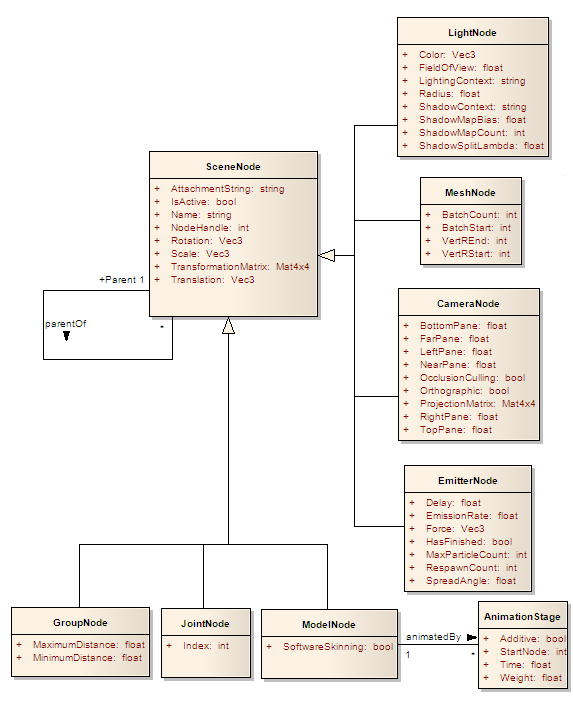
\includegraphics[scale=1.5]{images/Horde3DSceneGraph.png}
%\caption{Aufbau und Vererbungshierarchie des \Horde\ Szenengraphs}\label{fig:h3dscenegraph}
%\end{figure}

Der Szenengraph wird aus folgenden Knotentypen aufgebaut:

\begin{itemize}
	\item \textbf{Group}: Ein \emph{Group Node} hat keine Repr�sentation in der Szene, sondern fasst beliebig viele untergeordnete Knoten zusammen. Damit k�nnen beispielsweise alle untergeordneten Knoten auf einmal in der Szene verschoben, rotiert und ein- oder ausgeblendet werden. \emph{Root Node} ist von diesem Typ.
	\item \textbf{Camera}: In einer Szene k�nnen beliebig viele virtuelle Kameras vorhanden sein, die zum Zeichnen der Szene verwendet werden k�nnen. Insbesondere ist es m�glich, die Kamera einem animierten \emph{Joint Node} unterzuordnen, wobei die Kamera dann dem Bewegungsablauf der Animation folgt.
	\item \textbf{Light}: Ein \emph{Light Node} repr�sentiert eine Lichtquelle in der Szene. Derzeit werden von \Horde\ nur \emph{Spotlights} unterst�tzt. Ein Lichtknoten kann durch verschiedene Parameter -- wie Lichtfarbe, Reichweite und das An- oder Abschalten des Schattenwurfs -- an die Szene angepasst werden.
	\item \textbf{Model}: Ein \emph{Model Node} repr�sentiert ein 3D-Modell, welches aus einer Modellierungssoftware exportiert wurde. Es ist eine Menge von \emph{Mesh Node}s und \emph{Joint Node}s, welche das Aussehen und die Animation des Modells definieren.
	\item \textbf{Mesh}: Ein \emph{Mesh Node} enth�lt verschiedene Polygone, die zum Zeichnen eines 3D-Modells verwendet werden. Alle Polygone werden dabei mit dem gleichen Material gezeichnet.
	\item \textbf{Joint}: Eine Hierarchie von \emph{Joint Node}s repr�sentiert ein animierbares Skelett.
	\item \textbf{Emitter}: Ein \emph{Emitter Node} ist der Ursprungsort von Partikeln und kann verschiedene Eigenschaften der erzeugten Partikel beeinflussen.
	\item \textbf{Overlay}: Ein \emph{Overlay} ist eigentlich kein Teil des Szenengraphs. Es repr�sentiert eine zweidimensionale Grafik, die �ber die dargestellte Szene gezeichnet wird. Damit kann zum Beispiel ein \emph{Heads Up Display} realisiert werden. Auch das Zeichnen von Text wird von \Horde\ durch Verwendung von \emph{Overlay}s umgesetzt.
\end{itemize}

%\begin{figure}[h]
%\centering
%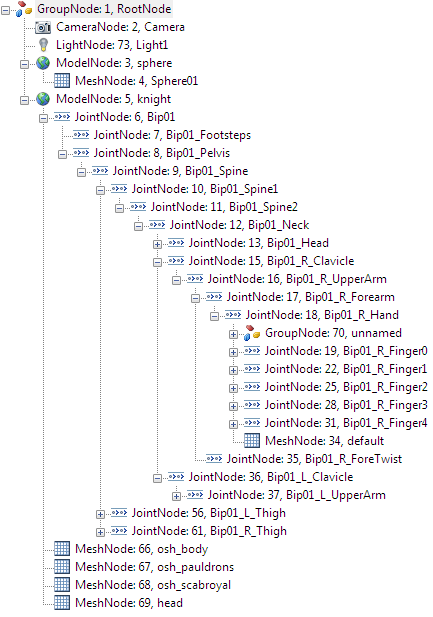
\includegraphics[scale=0.4]{images/KnightSampleSceneGraph.png}
%\caption{Ausschnitt des Szenengraphen des \textit{Horde3D} Knight Samples}\label{fig:knightscenegraph}
%\end{figure}

\subsection{Ressourcen-Verwaltung}
Ressourcen sind Daten, die zum Zeichnen der Szene ben�tigt werden. Dabei k�nnen mehrere \emph{Scene Node}s die gleichen Ressourcen verwenden \cite["`Basic Concepts, Resource Management"']{h3dmanual}. Der Horde3D Ressourcen Manager l�dt Ressourcen bei Bedarf und vergibt eindeutige \emph{Res Handles} zur Identifikation. Ressourcen k�nnen jederzeit neu geladen werden.

Horde3D kennt folgende Arten von Ressourcen:

\begin{itemize}
	\item \textbf{Scene Graph}: Eine \emph{Scene Graph Resource} enth�lt einen Szenengraph, der zum aktuellen Szenengraph als Ast hinzugef�gt werden kann.
	\item \textbf{Geometry}: Eine \emph{Geometry Resource} enth�lt Polygon-Daten f�r \emph{Mesh Nodes}. Neben den eigentlichen Eckpunkt-Koordinaten k�nnen auch weitere Daten -- wie Normalen, Tangenten, Texturkoordinaten, etc. -- enthalten sein.
	\item \textbf{Animation}: Eine \emph{Animation Resource} stellt Animationsdaten f�r \emph{Mesh} und \emph{Joint Nodes} bereit.
	\item \textbf{Pipeline}: Eine \textit{Pipeline Resource} ist ein XML-Dokument, das die erforderlichen Schritte zum Zeichnen der Szene beschreibt. Daf�r k�nnen zun�chst \emph{Render Targets} angelegt und die Engine-Konfiguration angepasst werden. Danach werden die einzelnen Schritte genau beschrieben: Zeichenreihenfolge der Material-Klassen, Lichtberechnungen, Verwenden von \emph{Render Targets} als Quelle und Ziel f�r Zeichenoperation, usw. Die Pipeline ist sehr flexibel und unterst�tzt sowohl \emph{Forward} als auch \emph{Deferred Shading}.
	\item \textbf{Material}: Eine \emph{Material Resource} definiert das Aussehen einer Oberfl�che. Sie legt fest, welche Texturen und welcher Shader zum Zeichnen verwendet werden.
	\item \textbf{Shader}: Eine \emph{Shader Resource} legt einen Kontext f�r die Ausf�hrung der Vertex und Fragment Shader auf der Grafikkarte fest. So kann ein Shader zum Beispiel einen Kontext f�r den \emph{Ambient Pass} und einen f�r den \emph{Deferred Lighting Pass} enthalten. Die Kontexte unterscheiden sich beim Code f�r Vertex und Fragment Shader und bei den Rendering-Optionen wie \emph{Depth Writes}, \emph{Alpha Writes}, etc.
	\item \textbf{Code}: Eine \emph{Code Resource} enth�lt Shader Code, der von mehreren Shadern verwendet werden kann.
	\item \textbf{Texture}: Eine \emph{Texture Resource} ist eine 2D-Textur oder \emph{Cube Map}, die beim Zeichnen von Oberfl�chen verwendet wird.
	\item \textbf{Particle Effect}: Eine \emph{Particle Effect Resource} legt die Gr��e, Farbe, Geschwindigkeit und Lebensdauer von Partikeln fest.
\end{itemize}

%\begin{figure}[h]
%\centering
%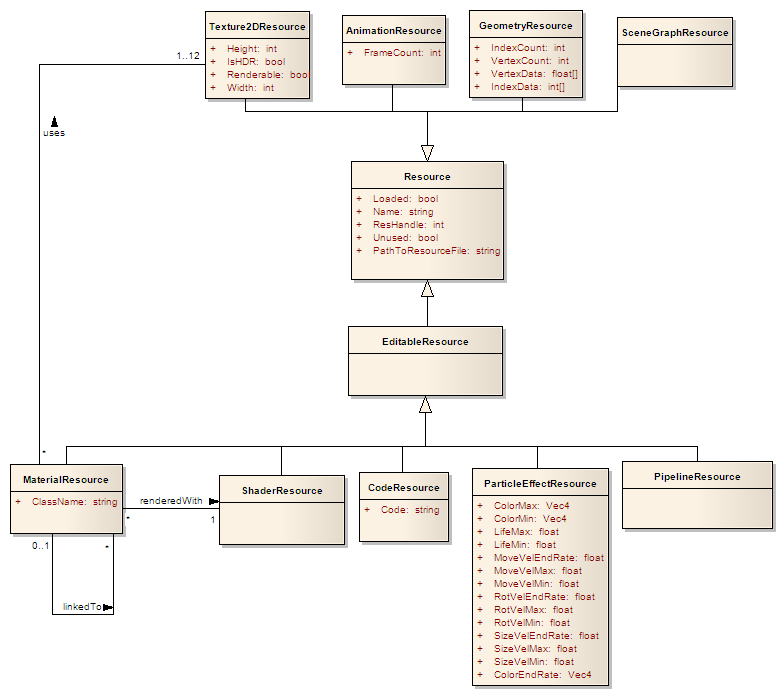
\includegraphics[scale=1.2]{images/Horde3DResources.png}
%\caption{Aufbau und Vererbungshierarchie der \Horde\ Ressourcen}\label{fig:h3dresources}
%\end{figure}

%Abbildung~\ref{fig:h3dresources} beschreibt den Aufbau und Vererbungshierarchie der Ressourcen. Die \textit{EditableResource}-Klasse ist in \textit{Horde3D} nicht vorhanden sondern soll zeigen, welche Arten von Ressourcen vom \DevEnv\ ge�ndert werden k�nnen. Einige Details der Shader und Pipelines sowie der Zusammenhang zwischen Ressourcen und \textit{Scene Nodes} werden in diesem Diagramm aus Gr�nden der �bersichtlichkeit allerdings nicht gezeigt.

\subsection{Eigenschaften der Horde3D-API}
Anwendungen k�nnen \Horde\ durch Einf�gen einer \emph{Header}-Datei und Linken gegen eine \emph{Dynamic Link Library} (DLL) einbinden. Obwohl die Engine in objekt-orientiertem \C++ entwickelt wurde, orientiert sich die �ffentliche Schnittstelle am Design der C-basierten Win32-API. Die Beta 3 von Version 1.0.0 hat gerade einmal 78 �ffentliche Funktionen. Dies erleichtert das Erlernen der API und das Erstellen von \emph{Bindings} f�r verschiedenen Programmiersprachen. Momentan werden C, \C++ und alle .NET-Sprachen offiziell unterst�tzt, weitere \textit{Bindings} werden derzeit von der Community entwickelt\footnote{Momentan entwickelt die Community zum Beispiel \textit{Bindings} f�r die Sprachen Python, D und Lua (\url{http://www.horde3d.org/wiki/index.php5?title=Language_Bindings}). Sogar f�r die funktionale Sprache Haskell gibt es \emph{Bindings} (\url{http://www.horde3d.org/forums/viewtopic.php?f=1&t=550}).}. Gegen�ber einer objekt-orientierten Schnittstelle, wie sie z.B. OGRE bietet, wird f�r manche Aufgaben jedoch mehr Code ben�tigt. Beispielsweise sind drei Funktionsaufrufe n�tig, um die Farbe eines \emph{Light Nodes} zu setzen; die Position, Rotation und Skalierung eines \emph{Nodes} k�nnen nicht einzeln ge�ndert werden und es gibt keine Vektor-Datentypen:

\lstset{language=C++} 
\begin{lstlisting}
// Horde3D::setNodeParamf muss dreimal aufgerufen werden, 
// um die Lichtfarbe auf Rot zu setzen.
Horde3D::setNodeParamf(light, LightNodeParams::Col_R, 1.0f);
Horde3D::setNodeParamf(light, LightNodeParams::Col_G, 0.0f);
Horde3D::setNodeParamf(light, LightNodeParams::Col_B, 0.0f);

// Diese Funktion �ndert die Position, Rotation und Skalierung von 
// 'node'. Daf�r m�ssen immer alle Werte skalar �bergeben werden.
Horde3D::setNodeTransform(node, 0, 20, 50, -30, 0, 0, 1, 1, 1);
\end{lstlisting}

%Wie sich sp�ter jedoch zeigen wird, erleichtert dieser API-Stil die Entwicklung des \DevEnvs.

Die Kern-API wurde schlank gehalten und ist ausreichend, um alle Features der Engine zu verwenden. Es gibt jedoch zus�tzlich die Horde3D \emph{Utility Library}, die verschiedene spezifische Funktionen zur Produktivit�tssteigerung bereitstellt. Mit dieser Bibliothek k�nnen zum Beispiel Ressourcen von der Festplatte geladen, Frame Statistiken angezeigt, der OpenGL-Kontext initialisiert oder Objekte der dargestellten Szene selektiert werden. Der Stil der Horde3DUtils-API entspricht dem der Kern-API \cite["`Utility Library API Reference"']{h3dmanual}.

\Horde\ bietet au�erdem einen Mechanismus an, um die Features der Engine durch Plugins zu erweitern. Diese verwenden nicht die �ffentliche API, sondern haben Zugriff auf die interne Klassenstruktur von \Horde. Um das zu erm�glichen, werden die Plugins zur Kompilierungszeit statisch in die \Horde\ DLL hineinkompiliert. Die �ffentlichen Schnittstellen der Plugins erweitern dann die Kern-API und k�nnen von allen \Horde-Anwendungen verwendet werden, die gegen die erweiterte DLL gelinkt werden \cite["`Basic Concepts"']{h3dmanual}.

\subsection{Fehlerbehandlung und Debug-Informationen}
Da C keine Ausnahmen unterst�tzt, zeigen \Horde-Funktionen Fehler durch spezielle Fehlerwerte auf; so gibt beispielsweise die Funktion \texttt{int getNodeType(NodeHandle)} im Fehlerfall den Wert \texttt{ResourceTypes::Undefined} zur�ck. Zus�tzlich verwaltet \Horde\ intern eine Liste aller aufgetretenen Fehler. Auch Ereignisse und Debug-Informationen werden protokolliert, wie zum Beispiel das Hinzuf�gen eines neuen \emph{Scene Nodes}, das Laden einer Ressource oder Probleme beim Kompilieren des Shader Codes. Die protokollierten Meldungen k�nnen aus der Engine ausgelesen werden, beziehungsweise �ber eine Funktion der \emph{Utility Library} direkt in eine Datei im HTML-Format auf die Festplatte geschrieben werden. Dies sind hilfreiche Informationen beim Entwickeln und Debuggen einer \Horde-Anwendung.

\subsection{Shader und Rendering-Pipeline}
\Horde\ baut auf OpenGL 2.0 auf, das eine hardware-unabh�ngige Schnittstelle f�r hardware-beschleunigte Rasterisierung von 3D-Grafik auf der Grafikkarte (GPU) bietet. Abbildung~\ref{fig:graphicsPipeline} gibt einen �berblick �ber die Pipeline-Architektur moderner GPUs. \texttt{Vertex Data} sind die untransformierten Daten der Eckpunkte der Geometrie der aktuellen Szene. \texttt{Primitive Data} verbindet diese Vertex-Daten zu einer Menge von Punkten, Linien, Dreiecken oder Polygonen. Die \texttt{Vertex Processing}-Stufe verwendet die Szenen- und Projektionsmatrizen zum Transformieren der Eckpunkte und berechnet gegebenenfalls weitere Daten pro Vertex, wie etwa Texturkoordinaten. In der \texttt{Geometry Processing}-Stufe findet die eigentliche Rasterisierung statt. Beim \texttt{Fragment Processing} werden die Farbwerte der Fragmente\footnote{Ein Pixel ist ein Bildpunkt auf dem Bildschirm. Ein Fragment hingegen ist ein Pixel, der eventuell nicht sichtbar ist. Im Allgemeinen werden pro Bild mehr Fragmente berechnet, als Pixel �berhaupt sichtbar sein k�nnen, weil manche Fragmente sp�ter unter gewissen Umst�nden wieder �berschrieben werden.} berechnet und in der \texttt{Fragment Rendering}-Stufe schlie�lich die Tiefen-, Alpha- und \emph{Stencil}-Tests durchgef�hrt. Sind die Tests f�r ein Fragment erfolgreich, so wird es in die Ausgabe-Textur geschrieben oder hineingemischt \cite{dxsdk}.

\begin{figure}[htp]
\centering
%trim=l b r t  	This option will crop the imported image by l from the left, b from the bottom, r from the right, and t  from the top. Where l, b, r and t are lengths. 
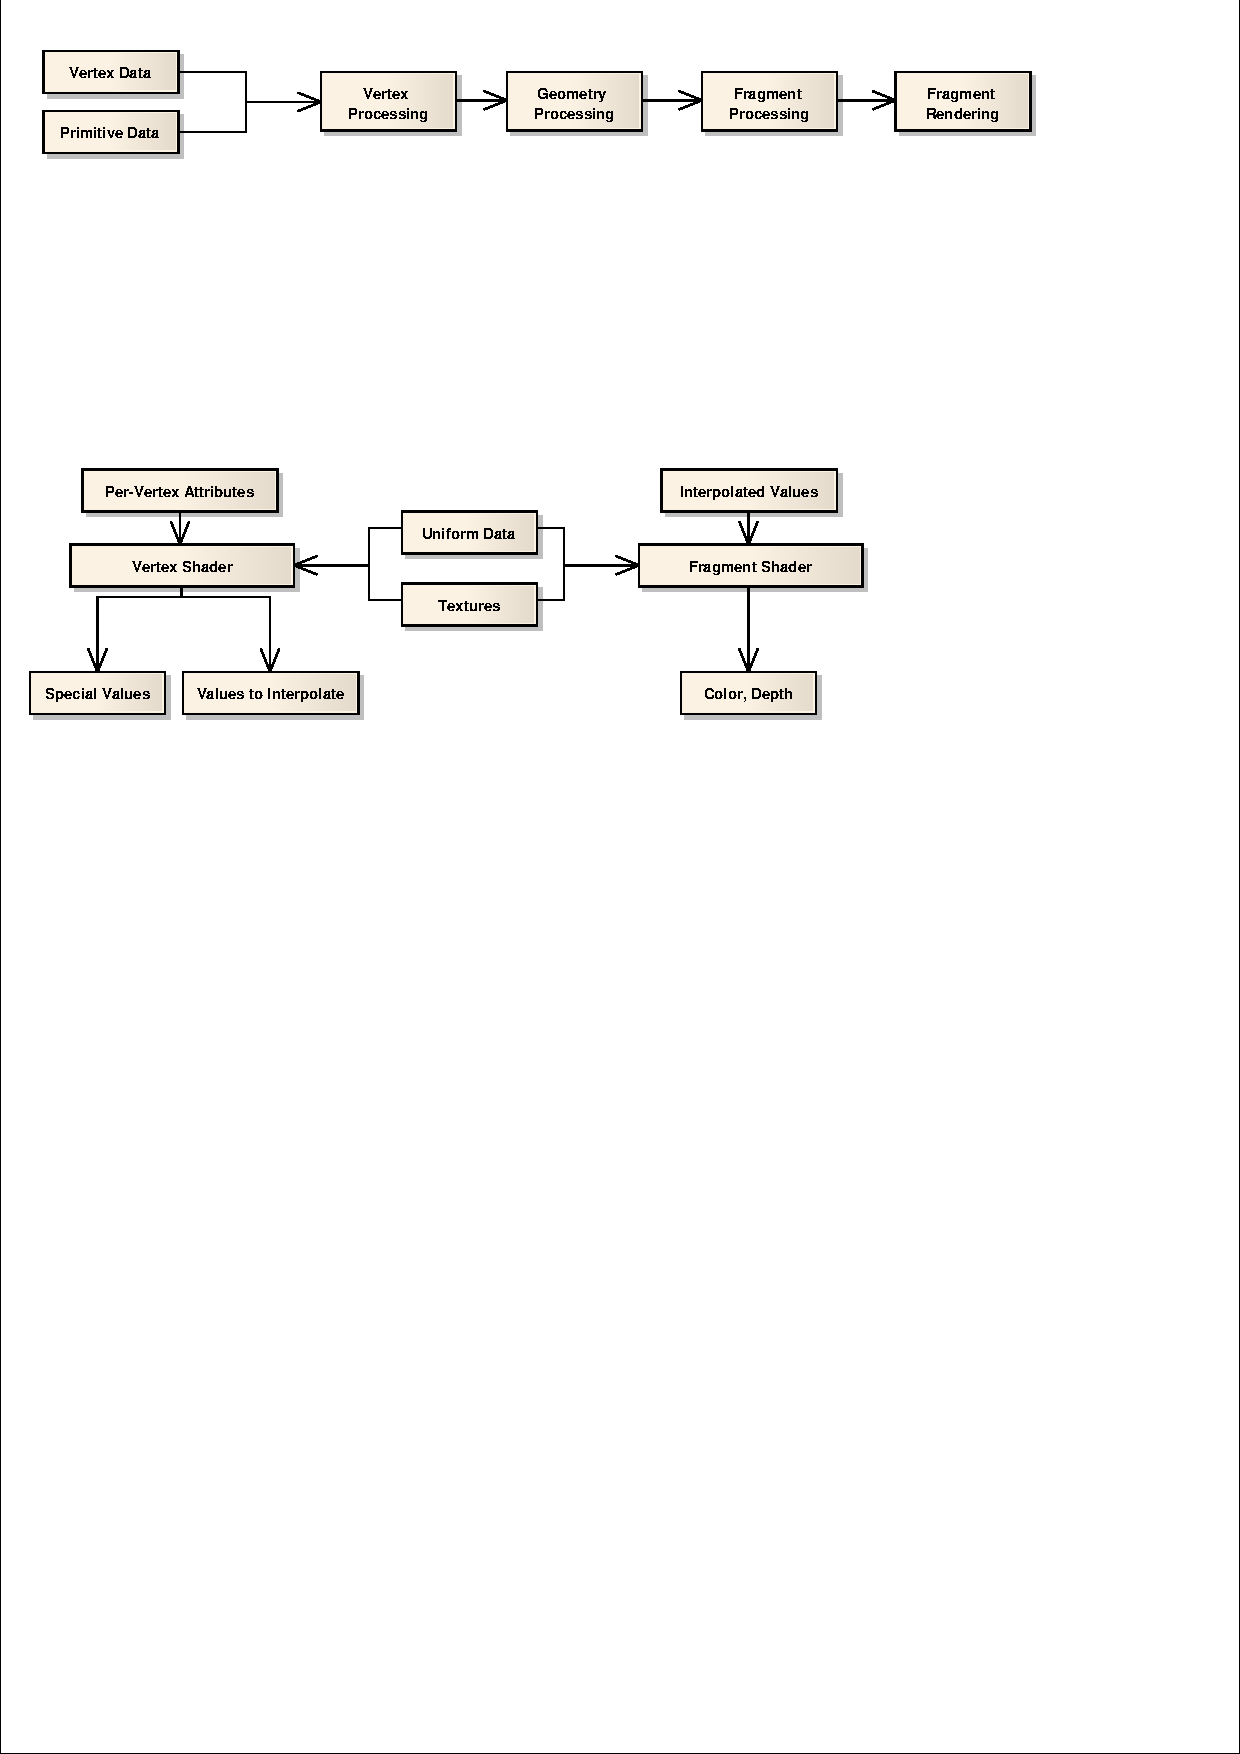
\includegraphics[trim = 5mm 265mm 30mm 5mm, clip, scale=0.7]{images/GraphicsPipeline.pdf}
\caption{Die Grafik-Pipeline von Direct3D 9 und OpenGL 2.0}\label{fig:graphicsPipeline}
\end{figure}

Bei modernen Grafikkarten k�nnen Fragmente nicht nur in den \emph{Backbuffer} geschrieben werden, sondern auch in \emph{Render Targets} (RTs). \emph{Render Targets} k�nnen im weiteren Verlauf wiederum als Eingabe f�r weitere Zeichenoperationen dienen. Dieses Vorgehen ist f�r eine Vielzahl moderner Effekte relevant; beispielsweise gibt es Effekte, die die zuvor berechneten Tiefeninformationen der Szene kennen m�ssen. Es ist auch m�glich, dass eine Zeichenoperation gleichzeitig verschiedene Werte in verschiedene RTs schreibt, also \emph{Multiple Render Target}s (MRTs) verwendet.

Seit DirectX 8 und den \texttt{ARB\_vertex\_program}- und \texttt{ARB\_fragment\_program}-Erweiterungen f�r OpenGL ist es m�glich, die \texttt{Vertex} und \texttt{Fragment Processing}-Stufen der Grafik-Pipeline mit Vertex respektive Fragment Shadern\footnote{Was unter OpenGL Fragment Shader hei�t, wird von Direct3D als Pixel Shader bezeichnet. Da die Fragment/Pixel Shader aber auf Fragmenten und nicht auf Pixeln arbeiten, ist die OpenGL-Terminologie zutreffender.} frei zu programmieren. Allerdings waren diese fr�hen APIs stark eingeschr�nkt; die Syntax der Shadersprache war an Assembler angelehnt und die Anzahl der Instruktionen pro Shader war sehr stark begrenzt. Durch die Weiterentwicklung der Grafik-Hardware konnten die Limitierungen jedoch zunehmend aufgehoben und mit HLSL, Cg und GLSL C-�hnliche Sprachen f�r die Shader-Programmierung entwickelt werden.

Die freie Programmierbarkeit der Vertex und Fragment Shader erm�glicht die Implementierung komplexer, hardware-beschleunigter Effekte. Ohne Shader w�ren die Effekte gar nicht oder nur mit sehr viel Programmieraufwand realisierbar. Der Erfolg der Shader zeigt sich auch dadurch, dass mit DirectX 10 sogar noch eine weitere Shader-Art, Geometry Shader, hinzugekommen ist. Zus�tzlich wurde die \emph{Fixed Function Pipeline}, also die Pipeline ohne frei programmierbare Shader, komplett entfernt. DirectX 11 wird noch drei weitere Shader-Arten hinzuf�gen und HLSL um die Unterst�tzung von objekt-orientierten Konzepten erweitern.

\Horde\ verwendet GLSL als Shadersprache und unterst�tzt derzeit offiziell nur Vertex und Fragment Shader. Wichtig f�r die Verwendung von Shadern ist das Verst�ndnis der Funktionsweise und der Kommunikationsm�glichkeiten zwischen den beiden Shader-Arten. 

Der Shader Code wird f�r jedes Vertex und jedes Fragment einzeln ausgef�hrt, insbesondere kennt ein Shader keine anderen Eckpunkte oder Fragmente. Nur durch diese Einschr�nkung kann der hohe Grad der Parallelisierbarkeit der Shader gew�hrleistet werden -- moderne Grafikkarten berechnen hunderte Shader gleichzeitig. 

\begin{figure}[htp]
\centering
%trim=l b r t  	This option will crop the imported image by l from the left, b from the bottom, r from the right, and t  from the top. Where l, b, r and t are lengths. 
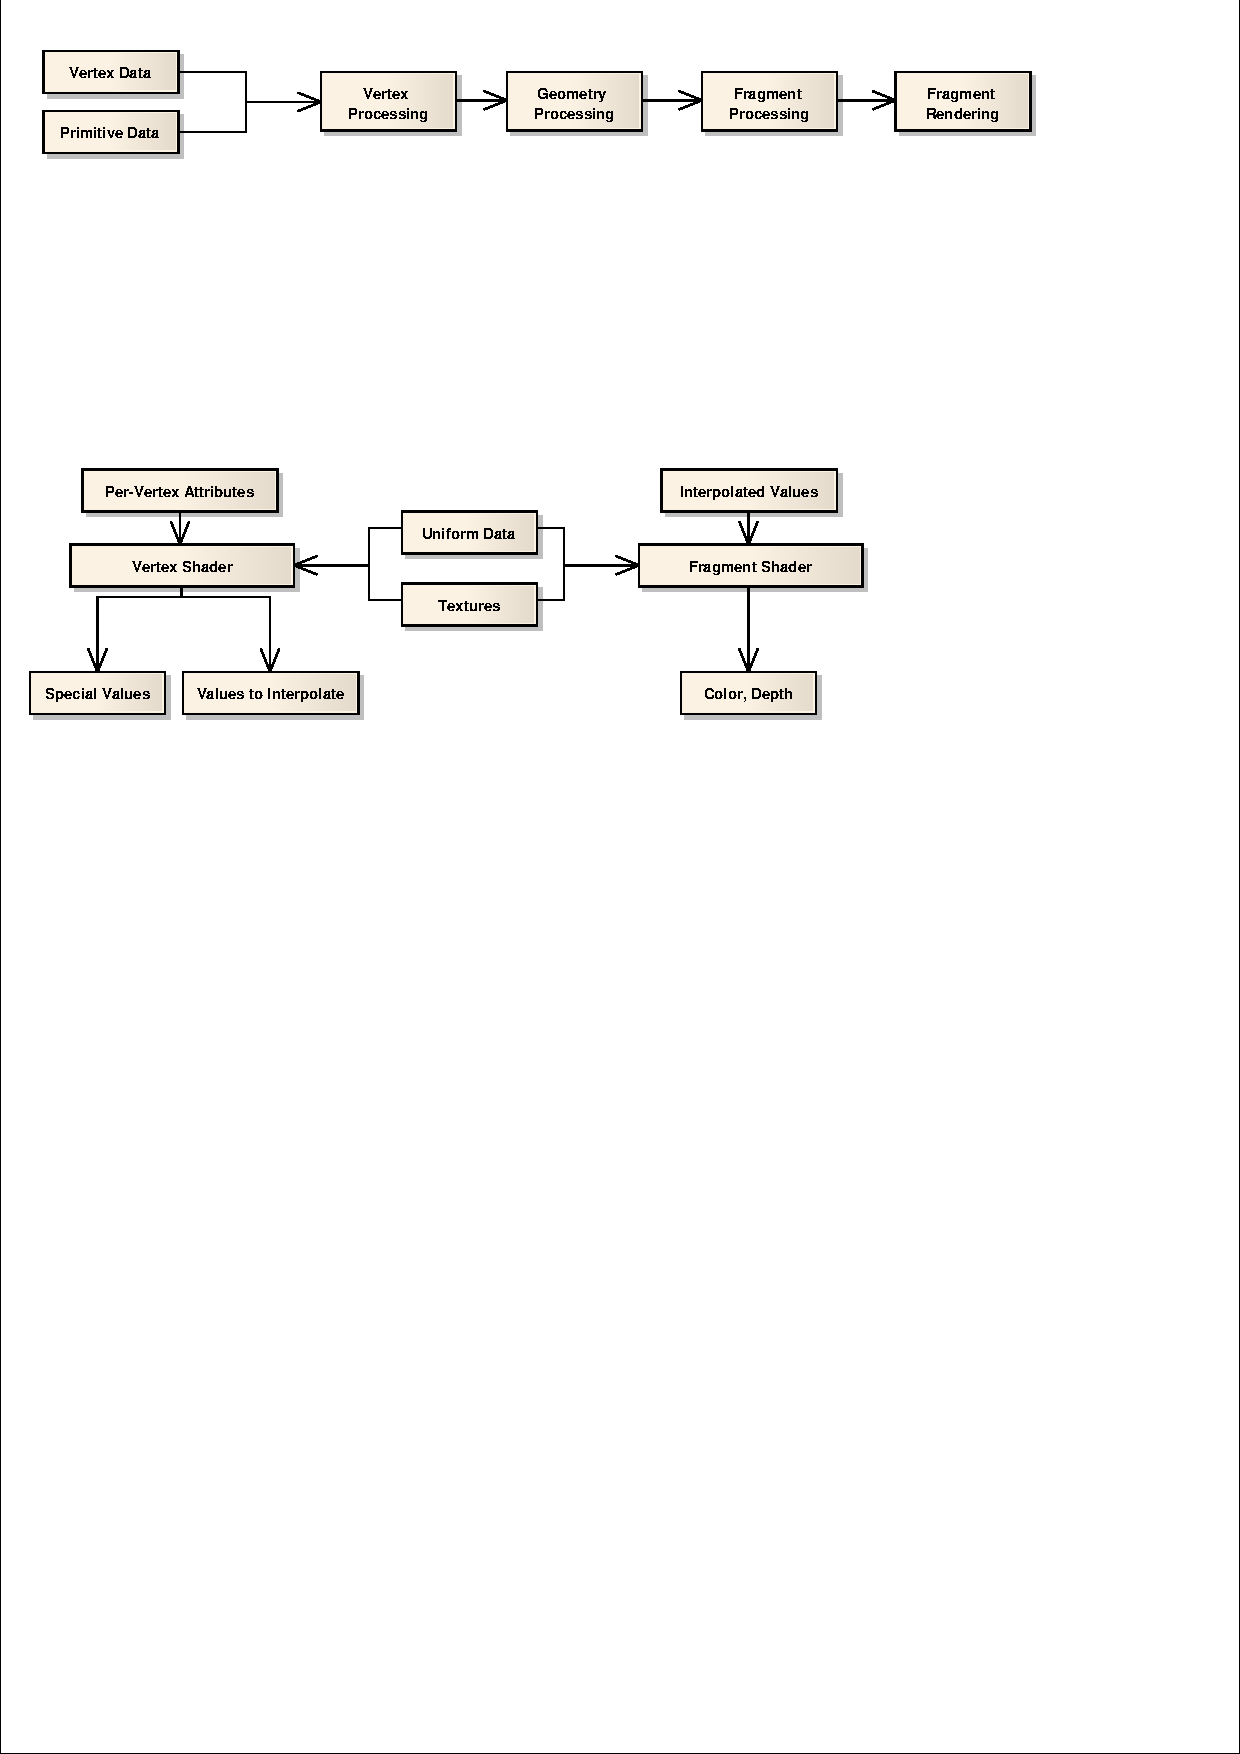
\includegraphics[trim = 5mm 170mm 45mm 75mm, clip, scale=0.7]{images/GraphicsPipeline.pdf}
\caption{Datenfluss zwischen Vertex und Fragment Shadern in OpenGL 2.0}\label{fig:shaderData}
\end{figure}

Abbildung~\ref{fig:shaderData} zeigt den Datenfluss zwischen den Shadern. Der Vertex Shader erh�lt Attribute f�r jedes Vertex, beispielsweise die Position und die Textur-Koordinaten. �ber \emph{Uniform}s k�nnen Vertex-unabh�ngige Daten, wie etwa die Transformations- und Projektionsmatrizen, Position der Lichtquelle, etc., abgerufen werden. Manche \emph{Uniform}s werden von OpenGL auch als \emph{built-in} Variablen zur Verf�gung gestellt\footnote{\emph{Built-in} Variablen wie beispielsweise Nebel- oder Lichtquellen-Einstellungen sind aus Effizienzgr�nden seit OpenGL 3.1 kein Teil des Standards mehr \cite{openglspec}.}. Auch Texturen k�nnen als Eingabe verwendet werden. Die Ausgabe erfolgt an spezielle Ausgabevariablen oder an Variablen, die �ber alle Eckpunkte eines Primitivs interpoliert und an den Fragment Shader weitergereicht werden. Der Fragment Shader kann mit diesen interpolierten Werten weiterrechnen und hat ebenfalls Zugriff auf die \emph{Uniforms}. Die Ausgabe des Fragment Shaders ist ein Farbwert und implizit auch ein Tiefenwert. Bei der Verwendung von MRTs werden mehrere Farbwerte ausgegeben \cite[S. 52]{astle}.

\Horde\ verwendet zwar GLSL, f�hrt aber ein XML-�hnliches Format ein, um die Ausdrucksst�rke der Shader zu erweitern. Die Erweiterung ist an die \emph{HLSL Effects} von Direct3D angelehnt. Dieses Framework erm�glicht es, f�r einen Effekt verschiedene Stufen zu definieren -- von \Horde\ als Kontext bezeichnet --, die jeweils unterschiedlichen Shader Code ausf�hren. Es k�nnen auch \emph{Uniforms} global definiert und Einstellungen f�r verwendete Texturen, wie zum Beispiel der anzuwendende Texturfilter, festgelegt werden. Jeder Kontext kann au�erdem die Vergleichsfunktion f�r den Tiefen- und Alphatest ausw�hlen und eine Funktion f�r das \emph{Blending} spezifizieren.

Das Pipeline-Konzept von \Horde\ geht jedoch �ber die \emph{HLSL Effects} hinaus. Pipelines erm�glichen die Definition verschiedener \emph{Render Targets} und die Festlegung deren Verwendung in den einzelnen Zeichenschritten als Ein- oder Ausgabe f�r die Shader. Es kann genau spezifiziert werden, welche Material-Klassen mit welchen Shader-Kontexten gezeichnet werden, wann \emph{Overlays} �ber die Szene gelegt werden und welche Art der Lichtberechnung -- \emph{Forward} oder \emph{Deferred Shading} -- verwendet wird. 
\section{Anforderungen an das System}
\begin{figure}[ht]
\centering
%trim=l b r t  	This option will crop the imported image by l from the left, b from the bottom, r from the right, and t  from the top. Where l, b, r and t are lengths. 
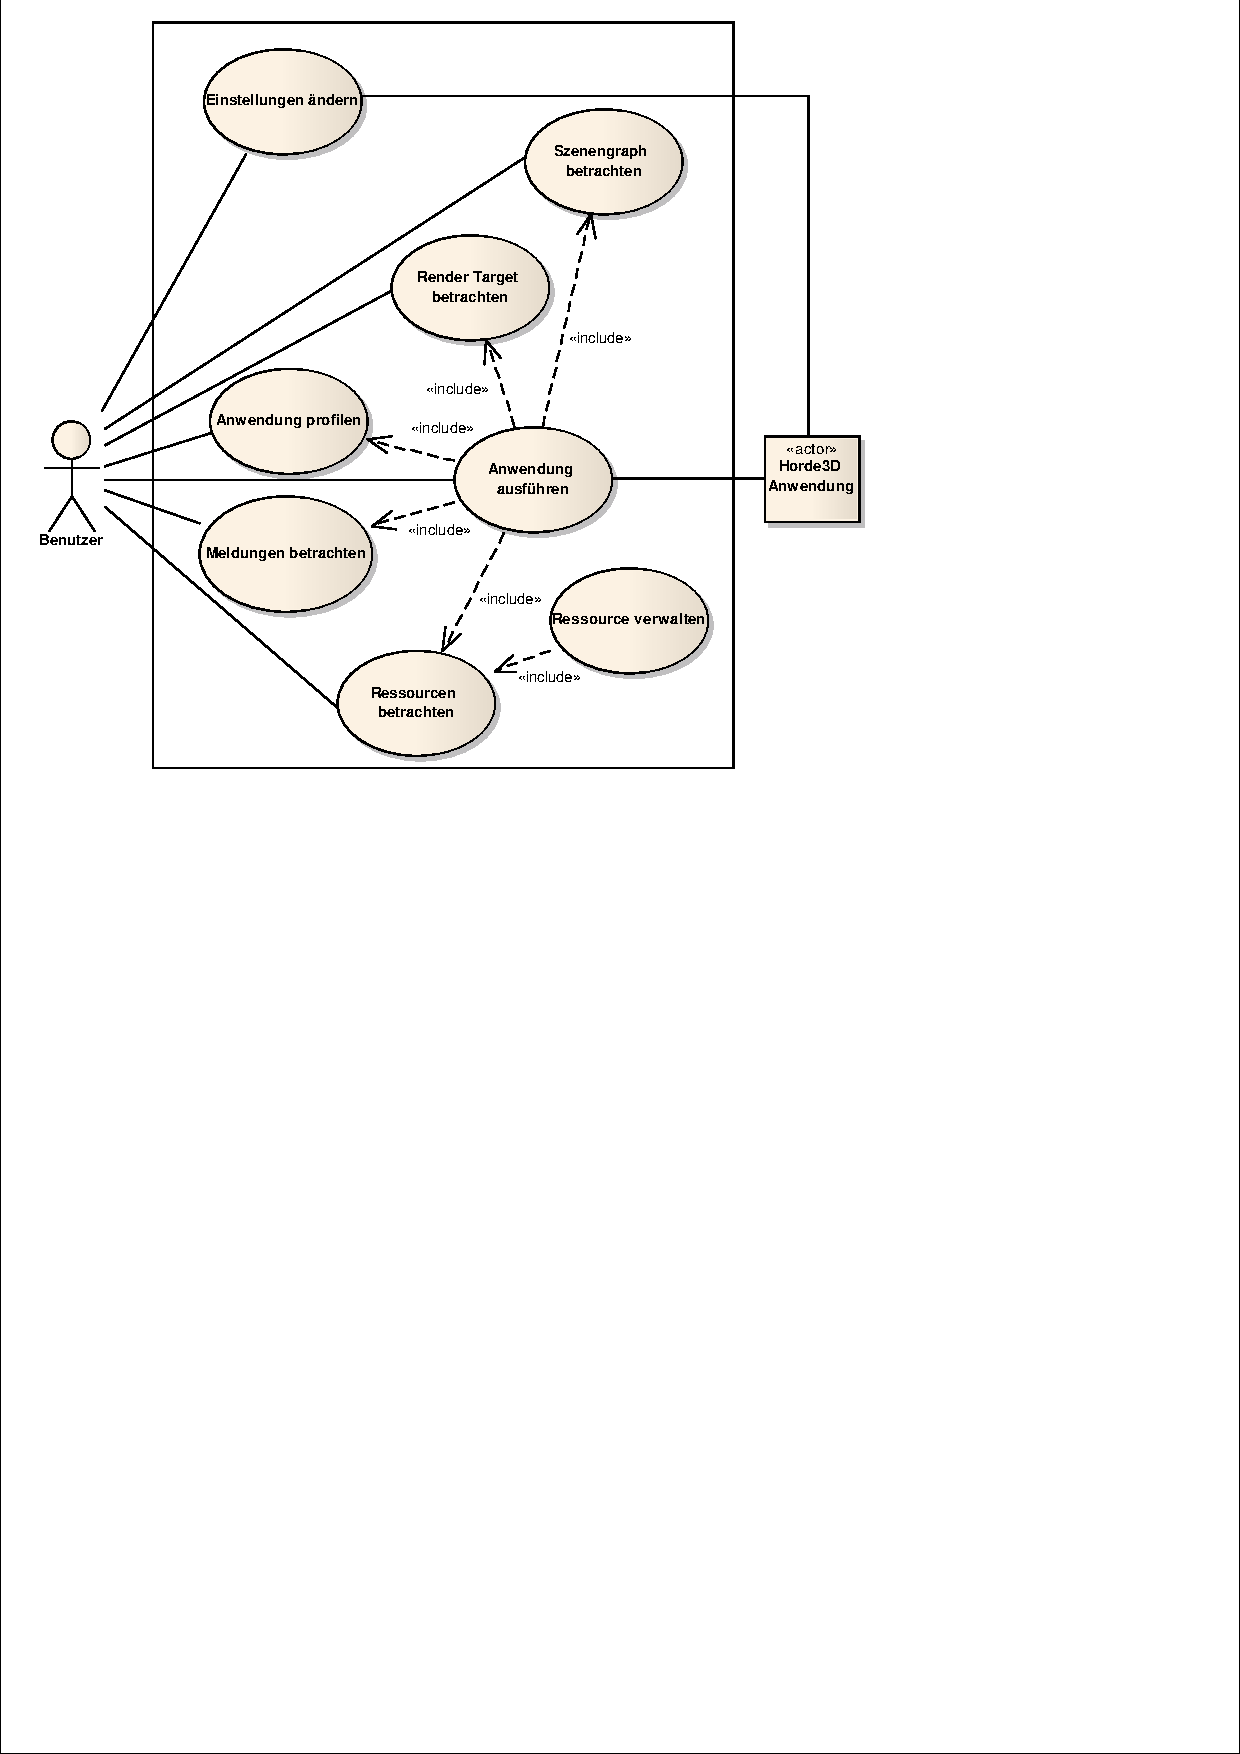
\includegraphics[trim = 1mm 160mm 60mm 1mm, clip, scale=0.7]{images/UseCase_Model.pdf}
\caption{Das \emph{Use Case} Modell des \DevEnvs}\label{fig:ucModel}
\end{figure}
Nach der Betrachtung der Funktionsweise von \Horde\ mussten die Anforderungen an das \DevEnv\ konkretisiert werden. Es kamen viele M�glichkeiten in Betracht, die Entwickler eines Spiels beim Erstellen, Optimieren und Feinabstimmen der Spieleeffekte zu unterst�tzen. Im Rahmen dieser Bachelorarbeit wurden deshalb ausschlie�lich diejenigen Anforderungen betrachtet, die speziell bei der Entwicklung von \SheepMeUp\ von Nutzen gewesen w�ren. Weitere denkbare Anforderungen und Erweiterungen des Systems werden in Kapitel~\ref{Ausblick} vorgestellt.

Abbildung~\ref{fig:ucModel} zeigt das \emph{Use Case} Modell des Systems. Die Anwendungsf�lle werden in den folgenden Abschnitten genauer beschrieben. Aktivit�tsdiagramme f�r die \emph{Use Cases} sind im Anhang abgebildet.

\subsection{Unabh�ngigkeit und Eigenst�ndigkeit}
Eine �bergeordnete Anforderung an das System war die Unabh�ngigkeit von der konkreten \Horde-Anwendung und von der Implementierung von \Horde. Um das \DevEnv\ beim Entwickeln einer Anwendung verwenden zu k�nnen, sollen keine �nderungen an der Anwendung n�tig sein; es sollen keine speziellen Funktionen aufgerufen oder gegen zus�tzliche Programmbibliotheken gelinkt werden m�ssen. 

Das System soll aber auch unabh�ngig von der Implementierung von \Horde\ sein. Dies verhindert das �berladen der Kern-API der Engine mit Tool-spezifischen Funktionen und erleichtert die Weiterentwicklung in getrennten Entwicklergruppen. 

Einzige Voraussetzung an \Horde-Anwendungen ist, dass eine unmodifizierte Horde3D DLL verwendet wird\footnote{Die derzeitige Implementierung unterst�tzt ohne erneutes Kompilieren keine modifzierten \Horde\ DLLs oder \Horde-Extensions.}.

\subsection{Absicherung vor unerw�nschtem Reverse-Engineering}
Mit dem \DevEnv\ k�nnen Einblicke in den Aufbau und in die Funktionsweise der Effekte von \Horde-Anwendung gewonnen werden. Dies k�nnte m�g\-lich\-er\-weise von manchen Anwendungsentwicklern unerw�nscht sein. Das System soll seine Dienste verweigern, wenn die Anwendung die Verwendung des \DevEnvs\ nicht explizit erlaubt. Um die Verwendung nur explizit zuzulassen, ist jedoch eine Modifizierung der Anwendung notwendig. Die damit einhergehende Verletzung des Ziels der Unabh�ngigkeit wird aber bewusst in Kauf genommen. So soll es f�r die Entwickler von \Horde-Anwendungen m�glich sein, das \DevEnv\ nur mit \emph{Debug Builds} ihrer Anwendung zu verwenden, wohingegen das Tool bei \emph{Release Builds} nicht verwendet werden kann.

Diese Anforderung wurde erst in einer sp�teren Iteration aufgenommen. Urspr�nglich regte Nicolas Schulz, der Entwickler von \Horde, die Entwicklung des Schutzmechanismus an.

\subsection{Konfigurieren und Ausf�hren der Horde3D-Anwendung}
Das System soll als eigenst�ndig ausf�hrbares Programm entwickelt werden, aus dem heraus die \Horde-Anwendung gestartet werden kann. Dadurch wird es erleichtert, die Anforderung der Unabh�ngigkeit zu erf�llen. Eine Alternative w�re, w�hrend der Ausf�hrung der Anwendung beim Dr�cken einer bestimmten Taste das \DevEnv\ zu laden und anzuzeigen. Dies h�tte jedoch �nderungen an der Anwendung oder an \Horde\ notwendig gemacht. Ein weiterer Vorteil der gew�hlten L�sung ist die M�glichkeit, das Tool sp�ter auch "`offline"' -- also ohne laufende \Horde-Anwendung -- verwenden zu k�nnen (siehe auch Kapitel~\ref{Ausblick}).

F�r den Start der \Horde-Anwendung sollen verschiedene Parameter eingestellt und gespeichert werden k�nnen: der Pfad zur \emph{Executable} der Anwendung, das Arbeitsverzeichnis, Kommandozeilenparameter sowie verschiedene implementierungsspezifische Details. Das \DevEnv\ soll eine Eingabemaske f�r diese Parameter bereitstellen und die Pfade auf Korrektheit �berpr�fen. Abbildung~\ref{fig:ucEinstellungenAendern} zeigt das Aktivit�tsdiagramm f�r die Konfiguration der Anwendungsparameter.

Abbildung~\ref{fig:ucAnwendungAusfuehren} erl�utert die Verwendung des \DevEnvs. Das System soll auf Wunsch des Benutzers die Anwendung starten. Der Benutzer soll grunds�tzlich jederzeit die M�glichkeit haben, die Anwendung wieder zu beenden. W�hrend das Programm l�uft, soll das System sofort alle von \Horde\ generierten Fehler-, Debug- und Informationsmeldungen in einer �bersicht anzeigen. Damit kann der Benutzer Probleme seiner Anwendung identifizieren, ohne die von den Horde3DUtils generierte HTML-Datei durchzusehen.

Hat die Anwendung einen Zustand erreicht, in dem der Benutzer die Anwendung anhalten m�chte, teilt er dies dem System mit. Das System soll die Anwendung anhalten und es dem Benutzer erm�glichen, die aktuelle Szene zu betrachten und Ressourcen zu �ndern, w�hrend sich die Szene selbst nicht �ndert. Dies kann im Allgemeinen, also ohne ein spezielles Anhalten der Anwendung, nicht garantiert werden: Ein Explosionseffekt in einem Spiel wird beispielsweise nur wenige Sekunden andauern. M�chte man den Effekt �ndern, so kann das Anhalten der Explosionsanimation beim Finetuning der Details der Explosion hilfreich sein.

W�hrend die Szene eingefroren ist, soll der Benutzer den Zustand der Anwendung analysieren k�nnen:

\begin{itemize}
	\item Das System soll alle bekannten Ressourcen auflisten. Falls eine Ressource editierbar ist, soll auf Wunsch die XML-Datei der Ressource geladen werden k�nnen. Der Benutzer soll die XML-Datei frei �ndern und die �nderungen speichern k�nnen. Anschlie�end soll das System die Szene mit der ge�nderten Ressource automatisch neu zeichnen.

	\item W�hrend der Ausf�hrung der Anwendung werden von \Horde\ Fehler- und Debug-Meldungen erzeugt. Das System soll diese bereits w�hrend der Ausf�hrung anzeigen und eine Filterung nach Wichtigkeit unterst�tzen.
	
	\item %Viele Shader-Effekte ben�tigen eine Kopie der aktuellen Szene. Daf�r werden Render Targets verwendet: Die Szene wird zun�chst in ein Render Target gezeichnet, aus welchem anschlie�end ein Shader die Szenendaten auslesen kann. Die Rendering Pipeline von \Horde\ unterst�tzt dieses Prinzip. 
	Mit dem Tool soll es m�glich sein, den Inhalt von aktiven \emph{Render Targets} zu betrachten. Da sich deren Daten, w�hrend die Anwendung nicht eingefroren ist, in jedem Frame �ndern k�nnen, soll das System automatisch in kurzen Zeitintervallen den dargestellten Inhalt aktualisieren.
	
		\item Das \DevEnv\ soll dem Benutzer eine einfache Profiling-Funktion anbieten. Das System soll die Aufrufe aller \Horde-Funktionen aufzeichnen und dem Benutzer anzeigen. Es soll dann eine Auswertung der gewonnenen Daten m�glich sein.

	\item Der Benutzer soll einen �berblick �ber den aktuellen Zustand des Szenengraphs erhalten k�nnen. Dazu soll der komplette Szenengraph als Baum dargestellt werden. Zu jedem \emph{Scene Node} sollen auf Wunsch weitere Details, wie etwa Typ, Name, Transformationswerte, etc., angezeigt werden. 
	
\end{itemize}

Anschlie�end kann der Benutzer entweder die Anwendung beenden oder mit der Ausf�hrung fortfahren. Anders als in Abbildung~\ref{fig:ucAnwendungAusfuehren} dargestellt, soll das System aber auch w�hrend der Weiterausf�hrung das �ndern von Ressourcen und Anzeigen des Inhalts von \emph{Render Targets} erlauben.

\subsection{Bearbeiten von Ressourcen und sofortiges Anzeigen der �nderungen}
Das System soll das Neuladen von ge�nderten Ressourcen ohne explizite Unterst�tzung der Anwendung erm�glichen. Das ist der wichtigste \emph{Use Case} des \DevEnvs: Jeder beliebige Shader- oder Partikel-basierte Spezialeffekt, jedes Material und jede Pipeline soll mit dem Tool zur Laufzeit der Anwendung, aber v�llig unabh�ngig von dieser, ge�ndert werden k�nnen. Die Anwendung soll beim n�chsten Zeichnen der Szene sofort die aktualisierten Ressourcen verwenden. Abbildungen \ref{fig:ucRessourcenBetrachten} und \ref{fig:ucRessourceVerwalten} zeigen den Ablauf dieses Anwendungsfalls. Zun�chst sollen alle Ressourcen in einer �bersicht angezeigt werden. Das System soll eine Filterm�glichkeit nach Ressourcen-Typ und -Name anbieten. Falls der Benutzer eine editierbare Ressource ausw�hlt, soll das System die zugrundeliegende XML-Datei der Ressource in einem Texteditor anzeigen. �nderungen an der XML-Datei sollen gespeichert und sofort an die \Horde-Anwendung �bermittelt werden k�nnen.

Beim Entwickeln der Kraftfeld- und Schockwellen-Effekte f�r \SheepMeUp\ war es wichtig, verschiedene Parameter der Effekte fein zu justieren und an das \emph{Look and Feel} des Spiels anzupassen. Das Ausblenden des Effekts, die Farbgebung, die Intensit�t und die Abspieldauer mussten von Hand eingestellt werden. Da weder \Horde\ noch \SheepMeUp\ ein automatisches Neuladen der Ressourcen unterst�tzen, war nur folgendes Vorgehen m�glich:

\begin{enumerate}
	\item Die XML-Datei des Effekts �ndern.
	\item Eventuell muss die Anwendung neu kompiliert und gelinkt werden\footnote{Bei der Entwicklung von \SheepMeUp\ war eine Neukompilierung erforderlich, wenn der Effekt von Werten aus der Anwendung abhing, die ebenfalls angepasst werden mussten. Dieses Problem kann das \DevEnv\ nicht l�sen. W�re \SheepMeUp\ nicht in \C++, sondern in \Csharp\ entwickelt worden, h�tte dieses Problem durch die \emph{Edit And Run}-Funktionalit�t von Visual Studio vermieden werden k�nnen.}.
	\item Das Spiel starten.
	\item Bis zur entsprechenden Stelle im Spiel spielen.
	\item Das Aussehen des Effekts beurteilen.
	\item Bei Nichtgefallen zur�ck zu Schritt 1.
\end{enumerate}

Dieser Prozess war zeitintensiv und unproduktiv. Das \DevEnv\ soll ein kontinuierliches Testen und Anpassen der Effekte erm�glichen und somit die Optimierung der Effekte leichter und schneller gestalten. Dies f�hrt zu einer entsprechenden Verbesserung der �sthetik des Spiels, und somit auch des Spiels insgesamt \cite[nach S. 89]{schell}. Das verbesserte Vorgehen l�sst sich wie folgt zusammenfassen:

\begin{enumerate}
	\item Das Spiel starten. 
	\item Bis zur entsprechenden Stelle im Spiel spielen.
	\item Das Aussehen des Effekts beurteilen.
	\item Die XML-Datei des Effekts �ndern, gegebenenfalls sogar unterst�tzt durch einen Designer.
	\item Bei Nichtgefallen zur�ck zu Schritt 3.
\end{enumerate}

W�hrend der Entwicklung des Systems zeigte sich au�erdem, dass das Shader-Format von \Horde\ bei komplexen Shadern un�bersichtlich werden kann. Aus diesem Grund wurde die Entwicklung eines visuellen Designers f�r \Horde-Shader in die Anforderungen aufgenommen. Im Rahmen dieser Bachelorarbeit soll die n�tige Infrastruktur f�r den Shader-Designer implementiert sowie die automatische Synchronisation des Designers und der XML-Datei umgesetzt werden. Der Designer soll das �ndern von bereits vorhandenen Shadern unterst�tzen; neue Shader sollen damit nicht angelegt werden k�nnen. In Kapitel~\ref{Ausblick} wird kurz auf die Limitierungen der derzeitigen Implementierung des Designers eingegangen.

\subsection{Anzeigen von Fehlern und Debug-Informationen}
\Horde\ generiert laufend Fehler- und Debug-Meldungen. Diese Meldungen sind die einzige M�glichkeit, mehr �ber aufgetretene Probleme beziehungsweise den derzeitigen internen Zustand der Engine zu erfahren. So traten bei der Entwicklung von \SheepMeUp\ mehrere Probleme auf, die nur mit Hilfe von \Horde-Fehlermeldungen gel�st werden konnten. Beispielsweise kam es in unregelm��igen Zeitabst�nden vor, dass scheinbar zuf�llig ausgew�hlte Schafe aus der Szene entfernt wurden. Im Anwendungscode gab es keine Hinweise, die dieses Problem erkl�ren konnten, da Schafe nur an einer genau definierten Stelle gel�scht wurden. Der entsprechende Code wurde beim Auftreten des Bugs aber nicht ausgef�hrt. Erst ein Blick in die von den Horde3DUtils generierte HTML-Datei f�hrte zur L�sung des Problems. Die Datei enthielt mehrere Warnungen �ber Versuche, \emph{Scene Nodes} �ber ung�ltige \emph{Node Handles} aus dem Szenengraph zu l�schen. Es stellte sich heraus, dass die Schafe sowohl vom Anwendungscode gel�scht wurden als auch von der verwendeten Game Engine der Universit�t Augsburg. Da \Horde\ nach dem L�schen eines Knoten dessen \emph{Node Handle} neu vergibt, wurde manchmal beim zweiten L�schen ein neu erzeugter Knoten im Szenengraph gel�scht. Mit diesem Wissen war das Problem leicht zu beheben und die HTML-Datei war anschlie�end frei von Fehlermeldungen.

Die Wichtigkeit der \Horde-Meldungen beim Entwickeln von Anwendungen ist nicht zu untersch�tzen. Problematisch ist, dass die Meldungen standardm��ig gar nicht angezeigt werden und von den Horde3DUtils nur in eine HTML-Datei geschrieben werden. Dort aber �bersieht man wichtige Informationen leicht. Im Zusammenhang mit dem Neuladen von aktualisierten Ressourcen sind die Meldungen aber auch noch aus einem weiteren Grund sehr wichtig. Sie zeigen n�mlich Probleme beim Neuladen der Ressourcen an, beispielsweise Syntaxfehler im GLSL-Code oder falsche Pfade zu referenzierten Ressourcen. 

Das System soll zum einen alle generierten Meldungen anzeigen und zum anderen auch das Filtern der Meldungen nach Wichtigkeit -- also Fehler, Warnung, Debug-Information -- unterst�tzen. Abbildung~\ref{fig:ucMeldungenBetrachten} zeigt das Aktivit�tsdiagramm f�r diesen \emph{Use Case}.

\subsection{Anzeigen von Render Targets}
F�r die Kraftfeld- und Schockwellen-Effekte verwendet \SheepMeUp\ mehrere \emph{Render Targets}, die die aktuellen Szenen-Daten, den Abstand eines Pixels zur Kamera und Ergebnisse verschiedener Zwischenberechnungen enthalten. Beim Programmieren der Shader w�re es hilfreich gewesen, direkt den Inhalt der RTs betrachten zu k�nnen. Als Workaround musste ein spezieller Schritt in die Pipeline-Konfiguration von \SheepMeUp\ eingef�hrt werden, der den Inhalt eines \emph{Render Targets} in den \emph{Backbuffer} kopiert und anzeigt. Das Spiel musste dann neu ge\-star\-tet und bis zur entsprechenden Stelle gespielt werden, um den Inhalt des RTs betrachten zu k�nnen. 

\emph{Render Targets} werden generell f�r die Grafikentwicklung immer wichtiger. \emph{Post Processing} Shader ben�tigen die gezeichnete Szene als Eingabe und das immer mehr in Mode kommende \emph{Deferred Shading} ben�tigt MRTs, um die Position jedes Pixels in der 3D-Welt, die Normale des Pixels und Materialeigenschaften zu speichern \cite[S. 255ff]{astle}. Daher soll das \DevEnv\ das Betrachten des RT-Inhalts vereinfachen. Wie Abbildung~\ref{fig:ucRenderTargetBetrachten} zeigt, soll das System dem Benutzer alle bekannten \emph{Render Targets} der eingefrorenen Szene zur Auswahl anbieten. Nachdem der Benutzer eines ausgew�hlt hat, soll das Tool den Inhalt des RTs darstellen. Da sich dieser im Allgemeinen in jedem Frame �ndert, soll das System immer die aktuellen Daten anzeigen. Dies soll auch w�hrend der Ausf�hrung der Anwendung m�glich sein. Bei der Implementierung dieses Features zeigte sich jedoch, dass ein Auslesen der RT-Daten in Echtzeit zu unperformant ist. Stattdessen soll ein Intervall eingestellt werden k�nnen, innerhalb dessen die angezeigten Daten aktualisiert werden.

\subsection{Profiling von Horde3D-Funktionen}
Grafikberechnungen sind sehr leistungshungrig, daher kann eine Optimierung des Codes lohnend sein -- eventuell gest�tzt durch Profiling-Tools wie Intels VTune\footnote{\url{http://software.intel.com/en-us/intel-vtune}}. Es ist keine Anforderung an das \DevEnv, etablierte Profiling-Tools zu ersetzen. Es soll aber m�glich sein, einen generellen �berblick �ber die Aufrufkosten von \Horde-Funktionen zu erhalten und entsprechende Auswertungen vorzunehmen. Das System soll eine Szene profilen k�nnen, indem es f�r einen Frame die Aufrufdaten der \Horde-Funktionen -- den Zeitpunkt des Aufrufs, die Ausf�hrungsdauer, sowie die Aufrufsreihenfolge und damit die Aufrufsh�ufigkeit -- protokolliert und dem Benutzer anzeigt. Der Benutzer soll die gewonnen Daten nach folgenden Kriterien analysieren k�nnen: Durchschnittliche Ausf�hrungsdauer einer Funktion, absolute Ausf�hrungsdauer einer Funktion und Anzahl der Aufrufe einer Funktion. Es soll au�erdem eine Aufruf-Historie dargestellt werden, die den zeitlichen Ablauf der Funktionsaufrufe repr�sentiert. Abbildung~\ref{fig:ucAnwendungProfilen} zeigt diesen Anwendungsfall als Aktivit�tsdiagramm.

\subsection{Anzeigen des Szenengraphs}
Im Rahmen der Bachelorarbeit soll eine Visualisierung des Zustands des Szenengraphs einer eingefrorenen Szene implementiert werden. Die Visualisierung soll dabei die Baumstruktur des Szenengraphs widerspiegeln. Wie Abbildung~\ref{fig:ucSzenengraphBetrachten} illustriert, sollen zu jedem \emph{Scene Node} auf Wunsch des Benutzers weitere Details angezeigt werden, wie beispielsweise der Typ des Knotens, sein Name oder seine Transformationswerte. F�r das Auslesen und Anzeigen der Daten soll die ben�tigte Infrastruktur entworfen und implementiert werden. In Kapitel~\ref{Ausblick} werden Ideen und M�glichkeiten f�r zuk�nftige Versionen des Tools vorgestellt, um diese Daten f�r interessante und hilfreiche Features zu verwenden.
\section{Konzeptmodell}

Abbildung~\ref{fig:domainModel} zeigt das Konzeptmodell des \DevEnvs. Die meisten Konzepte, ihre Abh�ngigkeiten und Spezialisierungshierarchien wurden von der Struktur und vom Aufbau von \Horde\ vorgegeben. Das Modell musste nur um die Konzepte \texttt{Horde3DApplication}, \texttt{FunctionCall} und \texttt{EditableResource} erweitert werden. Ersteres repr�sentiert die Anwendung, die vom Tool gestartet wird. \texttt{FunctionCall} wurden gegen�ber den System-Anforderungen noch um die Attribute \texttt{ReturnValue} und \texttt{Parameters} erweitert. In diesen beiden Attributen werden die Werte, die an die Funktion �bergeben beziehungsweise von ihr zur�ckgegeben werden, aufgezeichnet. Diese Daten wurden erst in einer sp�teren Iteration ins Konzeptmodell aufgenommen. Damit wird eine der in Kapitel~\ref{Ausblick} beschriebenen Erweiterungen bereits vorbereitet.

Im Konzeptmodell wurden alle Typen von \emph{Scene Nodes} als Spezialisierungen des abstrakten Konzepts \texttt{SceneNode} dargestellt. Bei den Ressourcen wurde zus�tzlich noch das Konzept der editierbaren Ressource hinzugef�gt, da das \DevEnv\ nur gewisse Ressourcentypen -- Materials, Pipelines, Shaders, Particle Effects und Code Ressourcen -- ver�ndern kann. Alle editierbaren Ressourcen sind durch das abstrakte Konzept \texttt{EditableResource} generalisiert, w�hrend alle anderen Ressourcen und \texttt{EditableResource} selbst Spezialisierungen des allgemeineren abstrakten Konzepts \texttt{Resource} sind.

Es wurden au�erdem die Beziehungen der einzelnen Ressourcen untereinander untersucht. Die Pipeline Konfiguration wurde auf einzelne Konzepte aufgeteilt, um m�glichst flexibel auf �nderungen und Erweiterungen der Pipeline in neuen \Horde-Versionen reagieren zu k�nnen. Au�erdem wurden die Assoziationen zwischen den \emph{Scene Nodes} und ihren ben�tigten Ressourcen eingezeichnet. Damit wird es sp�ter m�glich sein, f�r einen \emph{Scene Node} die verwendeten Ressourcen zu betrachten beziehungsweise f�r eine Ressource herauszufinden, von welchen Teilen des Szenengraphs sie verwendet wird. Diese detaillierte Analyse der Assoziationen zwischen den Konzepten war zwar nicht aufgrund der \emph{Use Cases} erforderlich, verbesserte aber das Verst�ndnis des Problembereichs und wird f�r einige der vorgeschlagenen Erweiterungen in Kapitel~\ref{Ausblick} ben�tigt.

Die \Horde-Konzepte, ihre Attribute und ihre Abh�ngigkeiten untereinander wurden aus der API-Beschreibung der \Horde-Dokumentation \cite["`Engine API Reference"']{h3dmanual} ermittelt. Da w�hrend der Entwicklung der Anwendung eine neue \Horde-Version erschien, mussten in einer sp�teren Iteration einige wenige Details der Konzepte ver�ndert werden. Hierbei machte sich allerdings die starke Modularisierung des Konzeptmodells positiv bemerkbar.
\section{Verwandte Softwaretools}\label{abgrenzung}
Neben dem \DevEnv\ gibt es eine Reihe weiterer Tools mit dem Ziel, die Entwicklung von 3D-Anwendungen zu vereinfachen und zu beschleunigen. Dabei unterscheiden sich die Tools nicht nur in ihrer Umsetzung, sondern vor allem auch darin, welches Problem sie zu l�sen versuchen. 

Nachdem die erste Iteration der Analyse abgeschlossen war, wurden die gefundenen Anforderungen mit bereits vorhandenen Tools verglichen. Teilweise dienten Ideen anderer Tools als Grundlage f�r Erweiterungen und Erg�nzungen der Anforderungen w�hrend der zweiten Iteration der Analyse-Phase. Es konnten aber auch Ideen f�r die Design- und Implementierungs-Phasen gewonnen werden.

Die folgenden Tools wurden eingehender betrachtet. Es wird kurz auf den Verwendungszweck, die Unterschiede zum \DevEnv\ und auf die f�r die weitere Entwicklung hilfreichen Ideen eingegangen.

\subsection{Horde3D Scene Editor}
Volker Wiendl entwickelte den Horde3D Scene Editor \cite{h3dscenewiki} zum Erstellen und Manipulieren von Szenen. Die erstellten Szenen k�nnen als \emph{Scene Graph Resource} gespeichert und von anderen \Horde-Anwendung geladen und angezeigt werden. Die Hauptaufgabe des Tools unterscheidet sich somit grundlegend von den Anforderungen an das \DevEnv. Es gibt jedoch auch �berschneidungen, da der Editor auch Unterst�tzung f�r die Entwicklung von Effekten bietet:

\begin{itemize}
	\item Ressourcen, die au�erhalb des Editors ver�ndert werden, werden sofort neu geladen und die Szene mit den ge�nderten Ressourcen gezeichnet. Das \DevEnv\ bemerkt externe �nderungen der Ressourcen-Dateien derzeit nicht.
	\item Es ist ein Designer zum �ndern von Materialeigenschaften integriert. Das \DevEnv\ bietet hierf�r keinen Designer an, sondern erlaubt nur die direkte �nderung der XML-Datei des Materials. Allerdings bietet der Szenen-Editor keinen Designer f�r Shader an.
	\item Auch der Editor erlaubt das Anzeigen des Inhalts eines beliebigen \emph{Render Targets}. Jedoch wird der dargestellte Inhalt nicht automatisch aktualisiert, wenn sich die Szene �ndert.
	\item Der Editor verwendet \Horde\ zum Darstellen der Szene. Allerdings l�uft dabei nicht der Code der Anwendung mit, f�r die die Szene erstellt wird. Dies ist problematisch, wenn Shader-Effekte von Parametern abh�ngen, die vom Anwendungscode in jedem Frame neu gesetzt werden m�ssen. In \SheepMeUp\ betraf dies die Kraftfeld- und Schock\-wel\-len-Effekte, die von einem Zeitparameter abhingen. Da der Editor diesen Parameter nicht aktualisierte, wurden die Effekte innerhalb des Editors nicht korrekt dargestellt.
	\item Die Szene kann nicht eingefroren und in Ruhe betrachtet werden, was zum Beispiel das Entwickeln von kurzlebigen Partikeleffekten erschweren kann. Auch der Schockwellen-Effekt von \SheepMeUp\ wird nur etwa eine Sekunde lang angezeigt. Das Finetuning solcher Effekte wird durch das Einfrieren der Szene erleichtert.
	
	\item Der Szenen-Editor kann durch Plugins erweitert werden, wodurch prinzipiell auch der Anwendungscode im Editor mitlaufen k�nnte. Allerdings erfordert dies eine Anpassung der Anwendung an den Editor, was in vielen F�llen nicht erw�nscht ist. Als Alternative gibt es die Game Engine der Universit�t Augsburg\footnote{\url{http://mm-werkstatt.informatik.uni-augsburg.de/projects/GameEngine/doku.php}}, die eng mit dem Szenen-Editor verkn�pft ist und beispielsweise Plugins f�r Physik und Sound bietet. Um von diesen Plugins profitieren zu k�nnen, m�sste die Anwendung neben \Horde\ aber auch die Game Engine verwenden. Beim \DevEnv\ hingegen sollen alle Features unabh�ngig von der Anwendung verwendbar sein; es kann mit jeder beliebigen \Horde-Anwendung -- auch mit dem Szenen-Editor und der Game Engine -- zusammenarbeiten, ohne �nderungen am Code n�tig zu machen. Die \Horde-Anwendung wird dabei normal ausgef�hrt und bekommt von der Verwendung des \DevEnvs\ nichts mit.
	\item Der Szenen-Editor ist plattformunabh�ngig in \C++ und Qt implementiert. Das \DevEnv\ hingegen l�uft nur unter Windows, da das .NET Framework 3.5 Service Pack 1 vorausgesetzt wird und einige Windows-spezifische Funktionen und Bibliotheken verwendet werden. Jedoch ist eine Implementierung in \Csharp\ und .NET im Allgemeinen weniger fehleranf�llig, einfacher und schneller.
\end{itemize}

\subsection{PIX for Windows}

Microsofts DirectX SDK\footnote{\url{http://msdn.microsoft.com/en-us/directx/default.aspx}} enth�lt das Direct3D Debugging-Tool PIX for Windows. Die Hauptaufgabe von PIX ist das Auffinden von Problemen bei der Verwendung der Direct3D-API. %Abbildung~\ref{fig:pix} zeigt einen Screenshot aus einer Debugsession mit PIX. 
Es wird eine Historie aller Direct3D Funktionsaufrufe angezeigt, sowie wichtige Daten �ber alle allozierten Direct3D-Ressourcen wie \emph{Vertex Buffer}, \emph{Index Buffer}, Texturen oder \emph{Render Targets}. Man kann sich den Inhalt eines \emph{Render Targets} anzeigen und die Szene schrittweise -- also \emph{Render Call} f�r \emph{Render Call} -- zeichnen lassen. Besonders hilfreich ist die M�glichkeit, Vertex, Geometry und Pixel Shader zu debuggen. Dazu w�hlt man einfach ein Vertex, Polygon oder Pixel in der Szene aus. PIX zeigt dann den Source Code des Shaders an und erm�glicht ein zeilenweises Durchlaufen des Codes und Anzeigen der Variablenwerte, wie man es vom Visual Studio Debugger gewohnt ist. Mit entsprechender Unterst�tzung des Grafikkartentreibers k�nnen auch verschiedene Metriken -- wie Auslastung der \emph{Raster Operation Units}, der \emph{Texture Mapping Units} sowie der Shadereinheiten der Grafikkarte -- f�r einen Frame untersucht und entsprechende Performanceoptimierungen an der Direct3D-Anwendung vorgenommen werden.
	
%\begin{figure}[ht]
%\centering
%%trim=l b r t  	This option will crop the imported image by l from the left, b from the bottom, r from the right, and t  from the top. Where l, b, r and t are lengths. 
%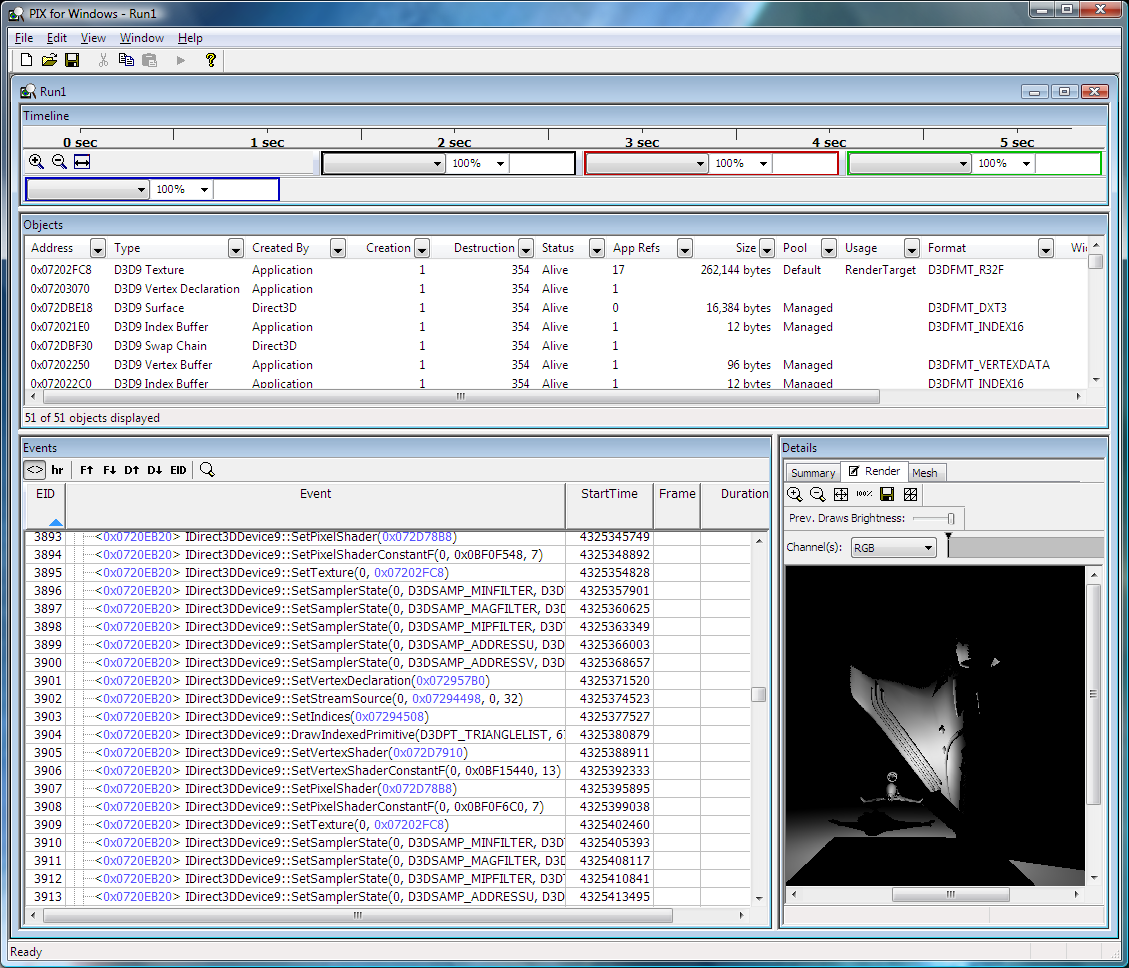
\includegraphics[scale=0.38]{images/PIX.png}
%\caption{Debuggen von Direct3D Anwendungen mit Microsofts  PIX for Windows}\label{fig:pix}
%\end{figure}
%	
\Horde\ hat derzeit nur einen OpenGL Renderpfad und somit ist die Verwendung von PIX f�r \Horde-Anwendungen unm�glich. Die Ziele des \DevEnvs\ unterscheiden sich allerdings haupts�chlich im Abstraktionslevel von den Zielen des Microsoft Tools: Beide Tools erlauben die Betrachtung des Zustands einer Software, die eine entsprechende API verwendet. Bei PIX ist diese API Direct3D, beim \DevEnv\ ist es \Horde. Insbesondere stammt die Idee der Funktionsaufruf-Historie und -Performanceauswertung aus PIX.
	
\subsection{NVIDIA PerfHUD}
NVIDIA PerfHUD\footnote{\url{http://developer.nvidia.com/nvperfhud_home.html}} ist ebenfalls ein Tool zum Debuggen von Direct3D-Anwendungen. Allerdings ist der Fokus nicht der gleiche wie bei PIX, sondern die Tools erg�nzen sich in ihren M�glichkeiten. So erlaubt PerfHUD ebenfalls ein schrittweises Zeichnen der Szene, unterst�tzt allerdings kein Shaderdebugging. Auch ist PerfHUD keine eigenst�ndige Anwendung wie PIX, sondern l�uft direkt in der zu debuggenden Anwendung mit. PerfHUDs Hauptaufgabe ist die Unterst�tzung der Performanceoptimierung und Auffinden von Flaschenh�lsen in der Grafik-Pipeline. Alle Performancecounter der NVIDIA Grafikkarten k�nnen mit dem Tool ausgelesen werden. Dies erm�glicht es beispielsweise, f�r einen \emph{Draw Call} die Auslastung der Shader Einheiten der Grafikkarte, die CPU-Auslastung durch den Grafikkartentreiber usw. zu ermitteln und auszuwerten.

Im Vergleich zum \DevEnv\ gibt es fast keine �berschneidungen in der Funktionalit�t. Jedoch macht es die Funktionsweise von PerfHUD erforderlich, die Szene einzufrieren. Der User Guide \cite[S. 11]{perfhud} gibt einen Hinweis darauf, dass dies technisch �ber ein "`Anhalten der Zeit"' gel�st wurde. Das \DevEnv\ verwendet einen analogen L�sungsansatz. Des Weiteren wurde Nicolas Schulz von diesem Tool inspiriert, als er den Schutz vor unerw�nschtem \emph{Reverse-Engineering} vorschlug. PerfHUD l�sst sich nur mit Anwendungen verwenden, die beim Starten ein spezielles Direct3D-\emph{Device} ausw�hlen. W�hlt die Anwendung in \emph{Release Builds} das PerfHUD-\emph{Device} nicht aus, verweigert das Tool seinen Dienst. Damit k�nnen Konkurrenzfirmen nicht herausfinden, wie die Anwendung eine Szene berechnet und auf welche Performancecharakteristika die Anwendung optimiert wurde.

\subsection{NVIDIA FxComposer und AMD RenderMonkey Toolsuite}
NVIDIA FxComposer\footnote{\url{http://developer.nvidia.com/object/fx_composer_home.html}} und AMD RenderMonkey Toolsuite\footnote{\url{http://developer.amd.com/GPU/RENDERMONKEY/Pages/default.aspx}} sind Entwicklungsumgebungen f�r Shader und Materials. Sie bieten eine Vorschau der erstellten Effekte an und k�nnen diese in verschiedene Formate f�r OpenGL- und Direct3D-Anwendungen exportieren. Allerdings gibt es derzeit keinen Exporter f�r das \Horde-Shaderformat und GLSL wird von beiden Tools nicht direkt unterst�tzt.

Im Gegensatz zum \DevEnv\ ist jedoch keine direkte Integration mit der Anwendung vorgesehen; die erstellten Shader und Materials k�nnen also nicht sofort in der Anwendung betrachtet werden. 
\section{Konklusion}
Es stellte sich als die richtige Entscheidung heraus, die Funktionsweise und den Aufbau von \Horde\ vor der eigentlichen Anforderungsanalyse genau zu untersuchen. Dadurch konnten wichtige Einblicke in den Problembereich gewonnen werden, da das Konzeptmodell fast komplett vorgegeben wurde. Zusammen mit den Erfahrungen aus der Entwicklung von SheepMeUp konnten viele Systemanforderungen gefunden werden, die sp�ter als hilfreich und wichtig best�tigt wurden.

%Das Konzeptmodell war eine gro�e Hilfe in der Design-Phase und wurde in sp�teren Iterationen fast nicht ver�ndert. Die Anforderungen an das System wurden im Design und in der Implementierung vollst�ndig umgesetzt und erwiesen sich als �u�ert hilfreich bei der Entwicklung eines Hitzeschimmer-Effekts f�r \SheepMeUp.

Die Betrachtung �hnlicher und verwandter Softwaretools best�tigte au�erdem, dass es f�r \Horde\ kein zum \DevEnv\ vergleichbares Tool gibt. Des Weiteren konnten einige Ideen der Tools in die Anforderungen, das Design oder die Implementierung des Systems integriert werden.

\chapter{Phase II: Design}\label{Design}

In der Design-Phase wurde die Architektur des Systems entworfen. Ausgehend von den Erkenntnissen der Analyse-Phase wurden zun�chst wichtige, grundlegende Entscheidungen gef�llt und schlie�lich ein Designklassen-Diagramm erstellt. F�r einige wichtige Operationen wurden au�erdem Sequenzdiagramme angefertigt, um weitere Einblicke in die Funktionsweise des Systems zu gewinnen. F�r die Anbindung der GUI wurde ein eigenst�ndiges Framework entwickelt, f�r das es ein eigenes Designklassen-Diagramm gibt.

\section{Grundlegende Entscheidungen}\label{decisions}	
Eine Anforderung an das System war die Unabh�ngigkeit von \Horde\ und der Anwendung des Benutzers. Bereits in der Design-Phase musste daher sichergestellt werden, dass die Implementierung keine �nderungen an \Horde\ oder der Benutzeranwendung voraussetzt. Die \emph{Use Cases} fordern zus�tzlich, dass das System die Anwendung des Benutzers starten und beenden kann. Eine Client-Server-Architektur zwischen \DevEnv\ und Anwendung, welche  service-orientiert entworfen wurde, erf�llt diese Anforderungen. Was nun als Server bezeichnet wird, ist in diesem Fall allerdings nicht klar. F�r die \Horde-Anwendung spricht, dass sie die Daten h�lt, die von dem System ausgelesen und angezeigt werden. F�r das System spricht hingegen, dass es die ganze Zeit l�uft und die \Horde-Anwendung erst starten muss. Das Festlegen einer genauen Terminologie wird zus�tzlich durch den Einsatz eines DLL-\emph{Replacement}-Mechanismus erschwert. Die originale \Horde\ DLL wird durch eine modifizierte Version ersetzt, die alle \Horde-Funktionsaufrufe -- f�r die Anwendung v�llig transparent -- an die Original-DLL weiterleitet und intern noch zus�tzlichen Code ausf�hrt. Dadurch schleust das \DevEnv\ Code in die \Horde-Anwendung ein; das System l�uft sowohl server- als auch client-seitig. 

In den n�chsten Abschnitten wird nun folgende Terminologie verwendet: Mit "`\Horde-Anwendung"' ist die Anwendung des Benutzers gemeint, ohne DLL-\emph{Replacement}. "`Server"' bezeichnet den Code des \DevEnvs, der innerhalb des Prozesses der \Horde-Anwendung l�uft. "`Client"' oder "`Shell"' ist der Teil des Systems, der als eigenst�ndige Applikation lauff�hig ist und Server-Instanzen starten und beenden kann. 

\begin{figure}[ht]
\centering
%trim=l b r t  	This option will crop the imported image by l from the left, b from the bottom, r from the right, and t  from the top. Where l, b, r and t are lengths. 
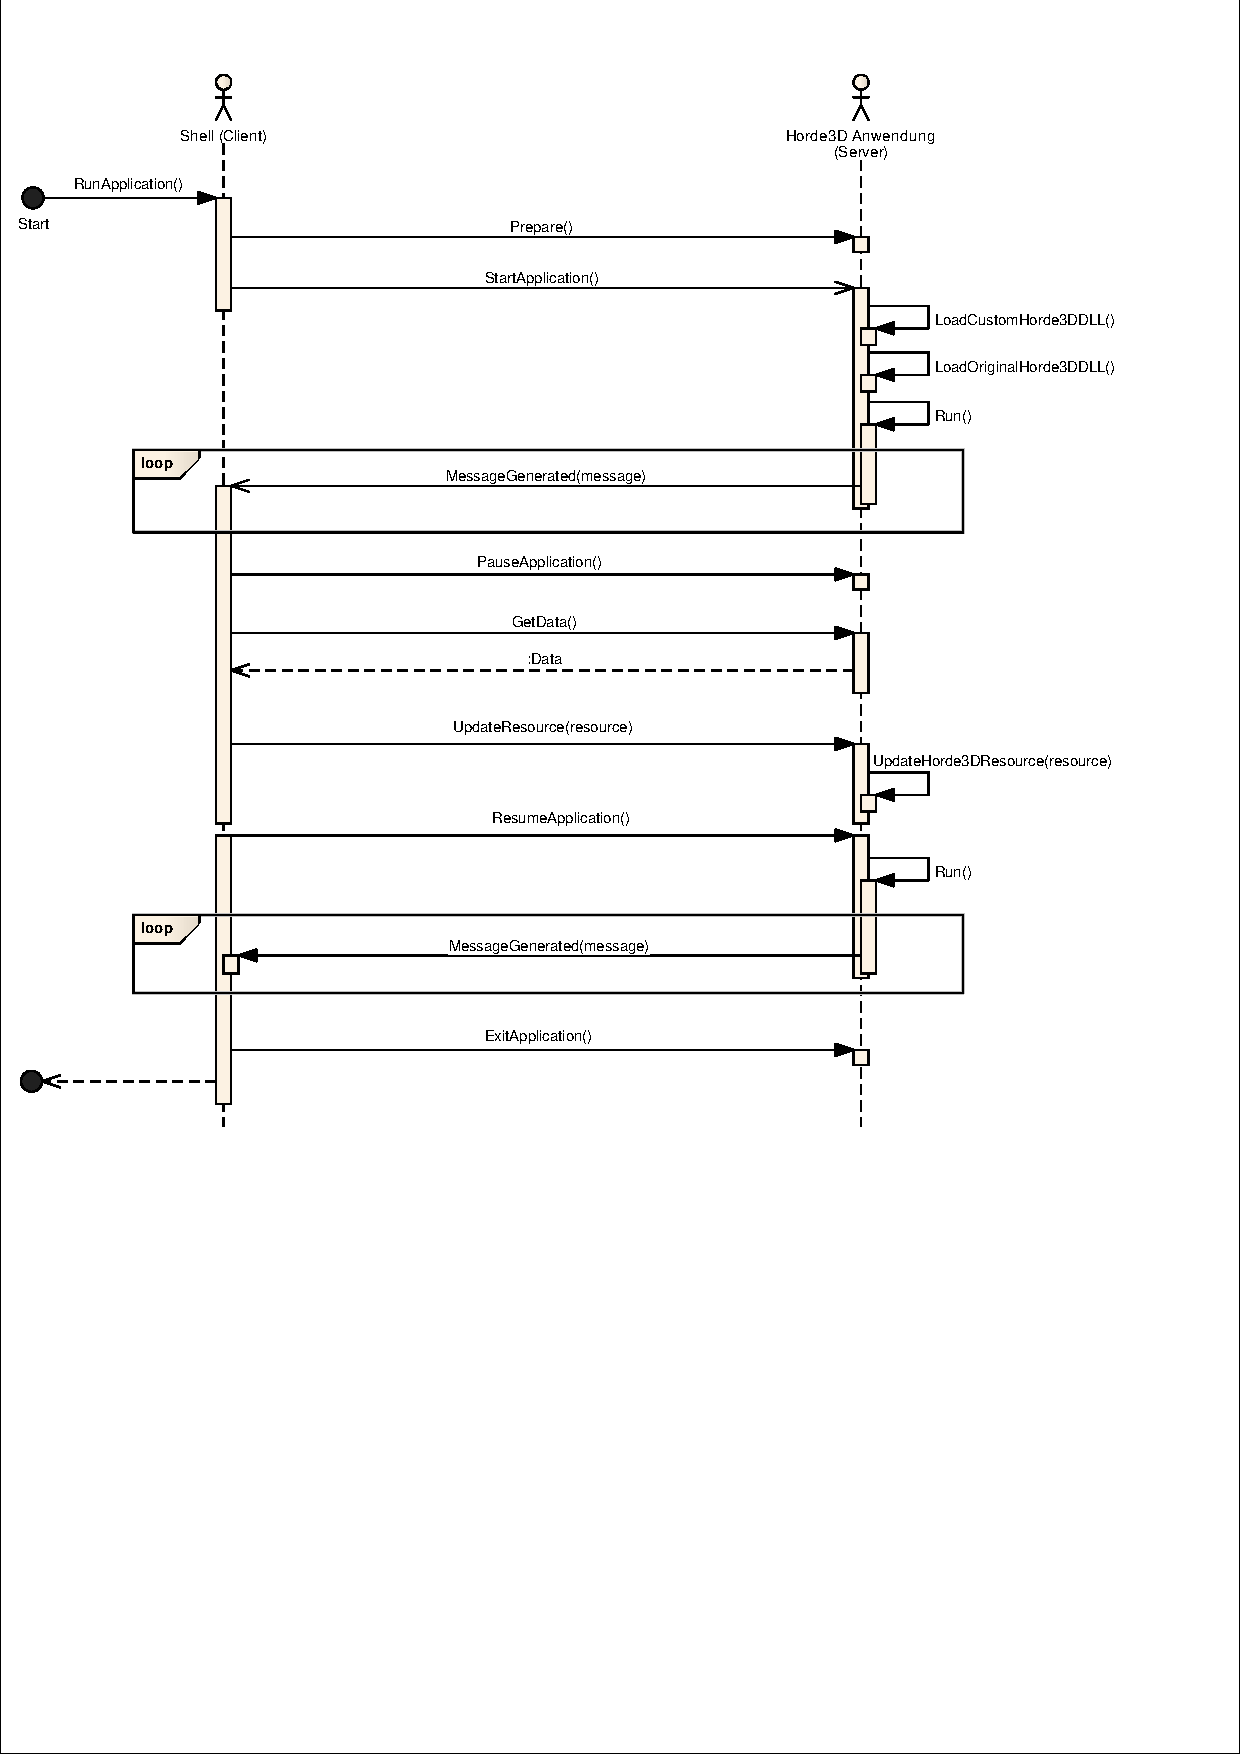
\includegraphics[trim = 3mm 100mm 15mm 12mm, clip, scale=0.7]{images/Prozess.pdf}
\caption{Interaktionen zwischen Client und Server an einem Beispiel}\label{fig:prozess}
\end{figure}

Abbildung~\ref{fig:prozess} verdeutlicht die Interaktionen zwischen Server und Client an einem Beispiel. Der Client wird dabei durch die Lebenslinie des linken Akteurs repr�sentiert, die rechte Lebenslinie repr�sentiert den Server. Die Shell f�hrt zun�chst ein paar vorbereitende Schritte durch -- unter anderem das DLL-\emph{Replacement} sowie einige Konfigurationsaufgaben -- und startet schlie�lich die \Horde-Anwendung. Anstelle der Original-DLL wird jedoch die modifizierte \Horde\ DLL geladen und initialisiert. W�hrend der Initialisierung wird schlie�lich die originale \Horde\ DLL in den Prozess geladen. Anschlie�end wird die Anwendung normal ausgef�hrt und alle von \Horde\ generierten Meldungen sofort an den Client geschickt.

Zu einem beliebigen Zeitpunkt weist der Benutzer die Shell an, die \Horde-Anwendung zu pausieren. Nun k�nnen alle relevanten Daten -- beispielsweise der aktuelle Zustand des Szenengraphs oder die derzeit bekannten Ressourcen -- aus dem Server ausgelesen werden. Anschlie�end wird eine Ressource ver�ndert und deren aktualisierte Daten wieder an den Server geschickt, der die entsprechende \Horde-Ressource aktualisiert. Danach wird die Anwendung fortgesetzt und beim Zeichnen die aktualisierte Ressource verwendet, bis die Shell den Server schlie�lich beendet.

\begin{figure}[ht]
\centering
%trim=l b r t  	This option will crop the imported image by l from the left, b from the bottom, r from the right, and t  from the top. Where l, b, r and t are lengths. 
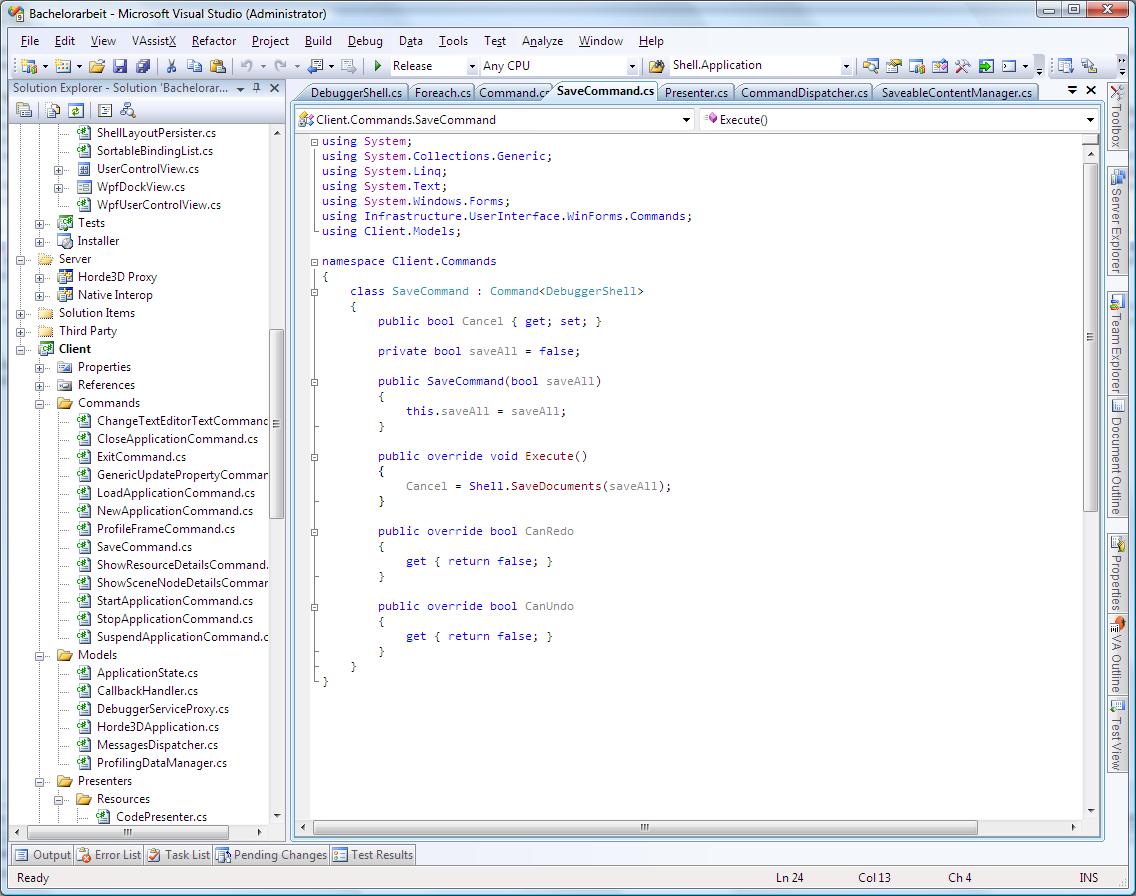
\includegraphics[scale=0.38]{images/VS.png}
\caption{Die grafische Benutzeroberfl�che von Visual Studio 2008}\label{fig:vs}
\end{figure}

Auch �ber die grafische Benutzeroberfl�che wurde bereits am Anfang der Design-Phase nachgedacht. Das \emph{User Interface} sollte sich an GUIs bekannter Entwicklungsumgebungen wie Visual Studio und Eclipse orientieren. Abbildung~\ref{fig:vs} verdeutlicht die geplante GUI am Beispiel von Visual Studio 2008: In der Mitte des \emph{Workspaces} werden mehrere Dokumente oder grafische Designer angezeigt. Oben gibt es die bereits von Windows bekannten Men�s und \emph{Toolbars}. An der rechten und an der unteren Seite sind verschiedene \emph{Tool Windows} versteckt, die erst beim Ber�hren mit der Maus sichtbar werden. Links ist das \emph{Solution Explorer Tool Window} "`angedockt"'. Die \emph{Tool Windows}, auch \emph{Dock Panes} genannt, k�nnen vom Benutzer frei positioniert sowie versteckt und wieder sichtbar gemacht werden. Es besteht auch die M�glichkeit, die \emph{Dock Panes} als eigenes Fenster (\emph{Floating Window}) �ber die Anwendung zu legen. Das vom Benutzer frei gew�hlte Layout wird gespeichert und beim Starten der Anwendung automatisch wiederhergestellt. 

Das \DevEnv\ wurde im Hinblick auf ein solches GUI-Design entworfen, da es weit verbreitet und bekannt ist und es dem Benutzer viele M�glichkeiten l�sst, die Oberfl�che an seine W�nsche und Vorlieben anzupassen. 

Zu Beginn der Design-Phase wurde auch entschieden, dass das System in \Csharp\ mit dem .NET Framework 3.5 Service Pack 1 implementiert wird. Dadurch ist das System zwar nur unter Windows lauff�hig, aufgrund der h�heren Produktivit�t gegen�ber einer Implementierung mit \C++ und Qt konnte bei der Entwicklung jedoch mehr Zeit in die eigentlich zu l�senden Probleme investiert werden. Diese Entscheidung wurde bereits zu diesem Zeitpunkt getroffen, damit schon in den Design-Artefakten .NET \emph{Properties} und \emph{Events} verwendet werden k�nnen, was die Darstellung erleichtert und verk�rzt. Da UML jedoch keine Unterst�tzung f�r diese Konzepte anbietet, wurden die entsprechenden UML-Attribute und -Operationen mit den Stereotypen \texttt{property} (\emph{Getter} und \emph{Setter} f�r Attribute), \texttt{event} (ein Ereignis, das auftreten kann) und \texttt{event property} (an diesem kann sich ein Objekt f�r ein \emph{Event} registrieren und deregistrieren) versehen.

All diese Entscheidungen hatten einen gro�en Einfluss auf den Gesamtentwurf des Systems. Deshalb war es wichtig zu �berpr�fen, ob die vorgestellten Konzepte �berhaupt wie geplant umsetzbar sind. Vor dem Entwurf der Design-Dokumente wurde daher ein Prototyp entwickelt, der die Machbarkeit der Konzepte �berpr�fte und als durchf�hrbar best�tigte.
\section{Angewandte Entwurfsmuster}
In der Softwareentwicklung gibt es f�r ein spezielles Architektur-Problem oftmals mehrere m�g\-liche L�sungswege. Diese sind je nach Situation besser oder schlechter geeignet. Eine der wichtigsten F�higkeiten eines Softwarearchitekten ist es daher, unterscheiden zu k�nnen, was f�r ein gegebenes Problem derjenige L�sungsansatz ist, der zum bestm�glichen Design f�hrt \cite[S. 4]{cpp}. Auf der anderen Seite gibt es in der Softwareentwicklung eine Vielzahl an wiederkehrenden Entwurfsproblemen, f�r die es bew�hrte L�sungsschablonen gibt. Die Schablonen, \emph{Design Patterns} oder Entwurfsmuster genannt, stellen eine allgemeine Vorlage zur Probleml�sung dar, die nur noch auf den spezifischen Kontext des Problems angepasst werden muss. Gut strukturierte, objekt-orientierte Softwarearchitekturen verwenden eine Vielzahl an unterschiedlichen \emph{Design Patterns} \cite{gangOfFour}.

Beim Design des \DevEnvs\ wurden verschiedene \emph{Design Patterns} angewandt, die im folgenden kurz vorgestellt werden. Bei der Vorstellung des Systemdesigns wird immer wieder auf die Verwendung der \emph{Patterns} zur L�sung eines Design-Problems hingewiesen.

\subsection{General Responsibility Assignment Software Patterns}
F�r die Zuweisung der Verantwortlichkeiten auf die einzelnen Klassen wurden einige der \emph{General Responsibility Assignment Software Patterns} verwendet \cite{grasp}. Da die \emph{Patterns} aber die Grundlage f�r objekt-orientierte Entw�rfe bilden und somit vielfach angewandt wurden, wird auf eine Instanziierung eines GRAS Entwurfsmuster im Designmodell nicht hingewiesen. Im folgenden seien die verwendeten \emph{GRAS Patterns} aber kurz vorgestellt:

\begin{itemize}
	\item \textbf{Expert:} \emph{Expert} ist das allgemeinste \emph{Pattern}. Diejenige Klasse sollte die Verantwortlichkeit erhalten, die alle ben�tigten Informationen daf�r besitzt.
	\item \textbf{Creator:} Das \emph{Creator Pattern} gibt Hinweise darauf, welche Klasse eine Instanz einer anderen Klasse erzeugen sollte. Ein Objekt $B$ sollte ein Objekt $A$ erzeugen, wenn beispielsweise $B$ eine Aggregation von $A$ ist, oder $B$ die ben�tigten Initialisierungsdaten f�r $A$ besitzt.
	\item \textbf{Low Coupling:} Mit Kopplung bezeichnet man das Ma� der Abh�ngigkeit einer Klasse von anderen Klassen. Eine niedrige Kopplung ist eines der wichtigsten Ziele von gutem objekt-orientierten Design, da es die Wiederverwendbarkeit erh�ht und auch die Verst�ndlichkeit und Wartbarkeit des Codes verbessert.
	\item \textbf{High Cohesion:} Die Koh�sion einer Klasse bezeichnet den semantischen Zusammenhang der Verantwortlichkeiten einer Klasse. Eine Klasse sollte m�glichst wenige verschiedene Aufgaben enthalten, um eine hohe Koh�sion zu erreichen. Dadurch werden die Klassen kleiner, die Verantwortlichkeiten einer Klasse genauer definiert und der Code damit insgesamt besser wartbar, verst�ndlich und wiederverwendbar. Jedoch steht das \emph{High Cohesion Pattern} im Widerspruch zu \emph{Low Coupling}. Beim Softwareentwurf muss daher eine angemessene Balance gefunden werden.
	\item \textbf{Polymorphismus:} Polymorphismus ist ein grundlegendes \emph{Pattern} der objekt-orientier\-ten Entwicklung, das von allen modernen objekt-orientierten Programmiersprachen direkt unterst�tzt wird. Durch die Verwendung von virtuellen und polymorphen Funktionen kann das Verhalten abh�ngig vom konkreten Typ der Klasse(n) ge�ndert werden.
	\item \textbf{Pure Fabrication:} Mit \emph{Pure Fabrication} bezeichnet man die Einf�hrung von Design-Klassen, die im Design eine spezielle Aufgabe �bernehmen, im Konzeptmodell aber nicht vorhanden sind.
\end{itemize}

\subsection{Gang of Four Design Patterns}
Der Entwurf des \DevEnvs\ verwendet einige der bekannten und oft eingesetzten \emph{Design Patterns} der \emph{Gang Of Four} \cite{gangOfFour}. Diejenigen dieser Entwurfsmuster, die f�r das Systemdesign eingesetzt wurden, seinen hier kurz erl�utert; an den entsprechenden Stellen wird auf ihre genaue Verwendung hingewiesen.

\begin{itemize}
	\item \textbf{Composite:} Das \emph{Composite Pattern} \cite[S. 163ff]{gangOfFour} f�gt mehrere Objekte in einer Baumstruktur zusammen, um eine Teil-Ganzes-Hierarchie zu repr�sentieren. Ein Knoten muss nicht unterscheiden, ob eines seiner Kinder ein Blatt oder wiederum ein Knoten mit weiteren Kindern ist. Primitive Objekte und Beh�lter k�nnen also uniform behandelt werden.
	\item \textbf{Facade:} Das \emph{Facade Pattern} \cite[S. 185ff]{gangOfFour} fasst verschiedene Interfaces unter einem gemeinsamen, einfacher benutzbaren Interface zusammen. Damit werden Komplexit�t und Abh�ngigkeiten reduziert, und somit das System besser wartbar.
	\item \textbf{Command:} Beim \emph{Command Pattern} \cite[S. 233ff]{gangOfFour} wird eine Operation durch ein Objekt gekapselt. Durchgef�hrte Operationen k�nnen parametrisiert und protokolliert werden. Dadurch wird es m�glich, Operationen sp�ter r�ckg�ngig zu machen.
	\item \textbf{Observer:} Das \emph{Observer Pattern} \cite[S. 293ff]{gangOfFour} wird direkt von zwei \Csharp-Sprachfeatures unterst�tzt: \emph{Delegates} und \emph{Events}. Objekte k�nnen einen speziellen \emph{Event Handler Delegate} f�r ein \emph{Event} eines (anderen) Objekts registrieren. L�st das Objekt das Ereignis aus, werden alle registrierten \emph{Delegates} automatisch ausgef�hrt. Das Objekt muss daf�r nicht wissen, welche Objekte oder ob �berhaupt Objekte an diesem Ereignis interessiert sind. Mit Hilfe dieses \emph{Patterns} kann eine \emph{One-To-Many}-Beziehung definiert werden, ohne zus�tzliche Abh�ngigkeiten einzuf�hren.
	\item \textbf{Singleton:} Das \emph{Singleton Design Pattern} \cite[S. 127ff]{gangOfFour} stellt sicher, dass es nur eine Instanz einer Klasse geben kann. F�r diese Instanz gibt es einen einzigen, globalen Zugriffspunkt.
	\item \textbf{Strategy:} Eine Menge von Algorithmen zur L�sung eines Problems kann mit dem \emph{Strategy Pattern} \cite[S. 315]{gangOfFour} gekapselt werden. Zur Laufzeit kann dann der am besten passende Algorithmus zur L�sung des Problems ausgew�hlt werden.
	\item \textbf{Decorator:} Das \emph{Decorator Pattern} \cite[S. 175]{gangOfFour} erm�glicht es, Verantwortlichkeiten dynamisch zur Laufzeit zu einem Objekt hinzuzuf�gen und wieder zu entfernen. Mit der klassische Vererbung hingegen k�nnen Verantwortlichkeiten nur statisch hinzugef�gt werden.
	\item \textbf{Template Method:} Beim \emph{Template Method Pattern} wird in einer Methode ein Algorithmus definiert, wobei manche Schritte als abstrakte oder virtuelle Methoden gekapselt sind. Abgeleitete Klassen m�ssen oder k�nnen diese Methoden �berschreiben und so einzelne Schritte, nicht aber die Struktur des Algorithmus, ver�ndern. Die Unterst�tzung von Lambda-Funktionen in \Csharp\ erm�glicht eine Variation des \emph{Patterns}: Dem Algorithmus werden Lambda-Funktionen �bergeben, die der Algorithmus an ausgewiesenen Stellen ausf�hrt. Die Lambda-Funktionen ersetzen somit die abstrakten oder virtuellen Methoden.
\end{itemize}

\subsection{Model-View-Presenter Design Pattern}
Die Anbindung der GUI an das System ist �ber das \emph{Model-View-Presenter Design Pattern} umgesetzt. Leider gibt es f�r dieses Entwurfsmuster keine genaue Definition; es gibt mehrere verschiedene Varianten und die Abgrenzung zum \emph{Model-View-Controller Pattern} ist ebenfalls nicht ganz klar \cite[Abschnitt "`Model-View-Controller and Model-View-Presenter Confusion"']{mvpconfusion}. Der gemeinsame Nenner ist lediglich die Separation der Anwendung in drei Bereiche: 

\begin{itemize}
	\item \textbf{Models:} Die Modelle sind die eigentlichen Businessobjekte der Anwendung aus dem Designmodell. Sie k�nnen gegebenenfalls mit dem \emph{Facade} oder \emph{Controller Pattern} gekapselt sein, um das Zugriffsinterface f�r die GUI-Anbindung zu vereinfachen.
	\item \textbf{Views:} Die \emph{Views} sind f�r die grafische Anzeige zust�ndig. Sie sind die einzigen Klassen, die Abh�ngigkeiten zum gew�hlten GUI-Framework wie Windows Forms oder der Windows Presentation Foundation haben. Die \emph{Views} zeigen die Daten der Modelle an; wie sie allerdings an die Daten kommen, ist nicht genau definiert.
	\item \textbf{Presenters:} Die Rolle der \emph{Presenter} ist ebenfalls nicht klar festgelegt. Fest steht, dass die \emph{Views} auf Benutzereingaben nicht selbst reagieren, sondern diese an ihren jeweiligen \emph{Presenter} weiterreichen. Ob ein \emph{Presenter} Daten an seine \emph{View} schicken darf, h�ngt von der verwendeten Variante des \emph{Model-View-Presenter Patterns} ab.
\end{itemize}

\begin{figure}[ht]
\centering
%trim=l b r t  	This option will crop the imported image by l from the left, b from the bottom, r from the right, and t  from the top. Where l, b, r and t are lengths. 
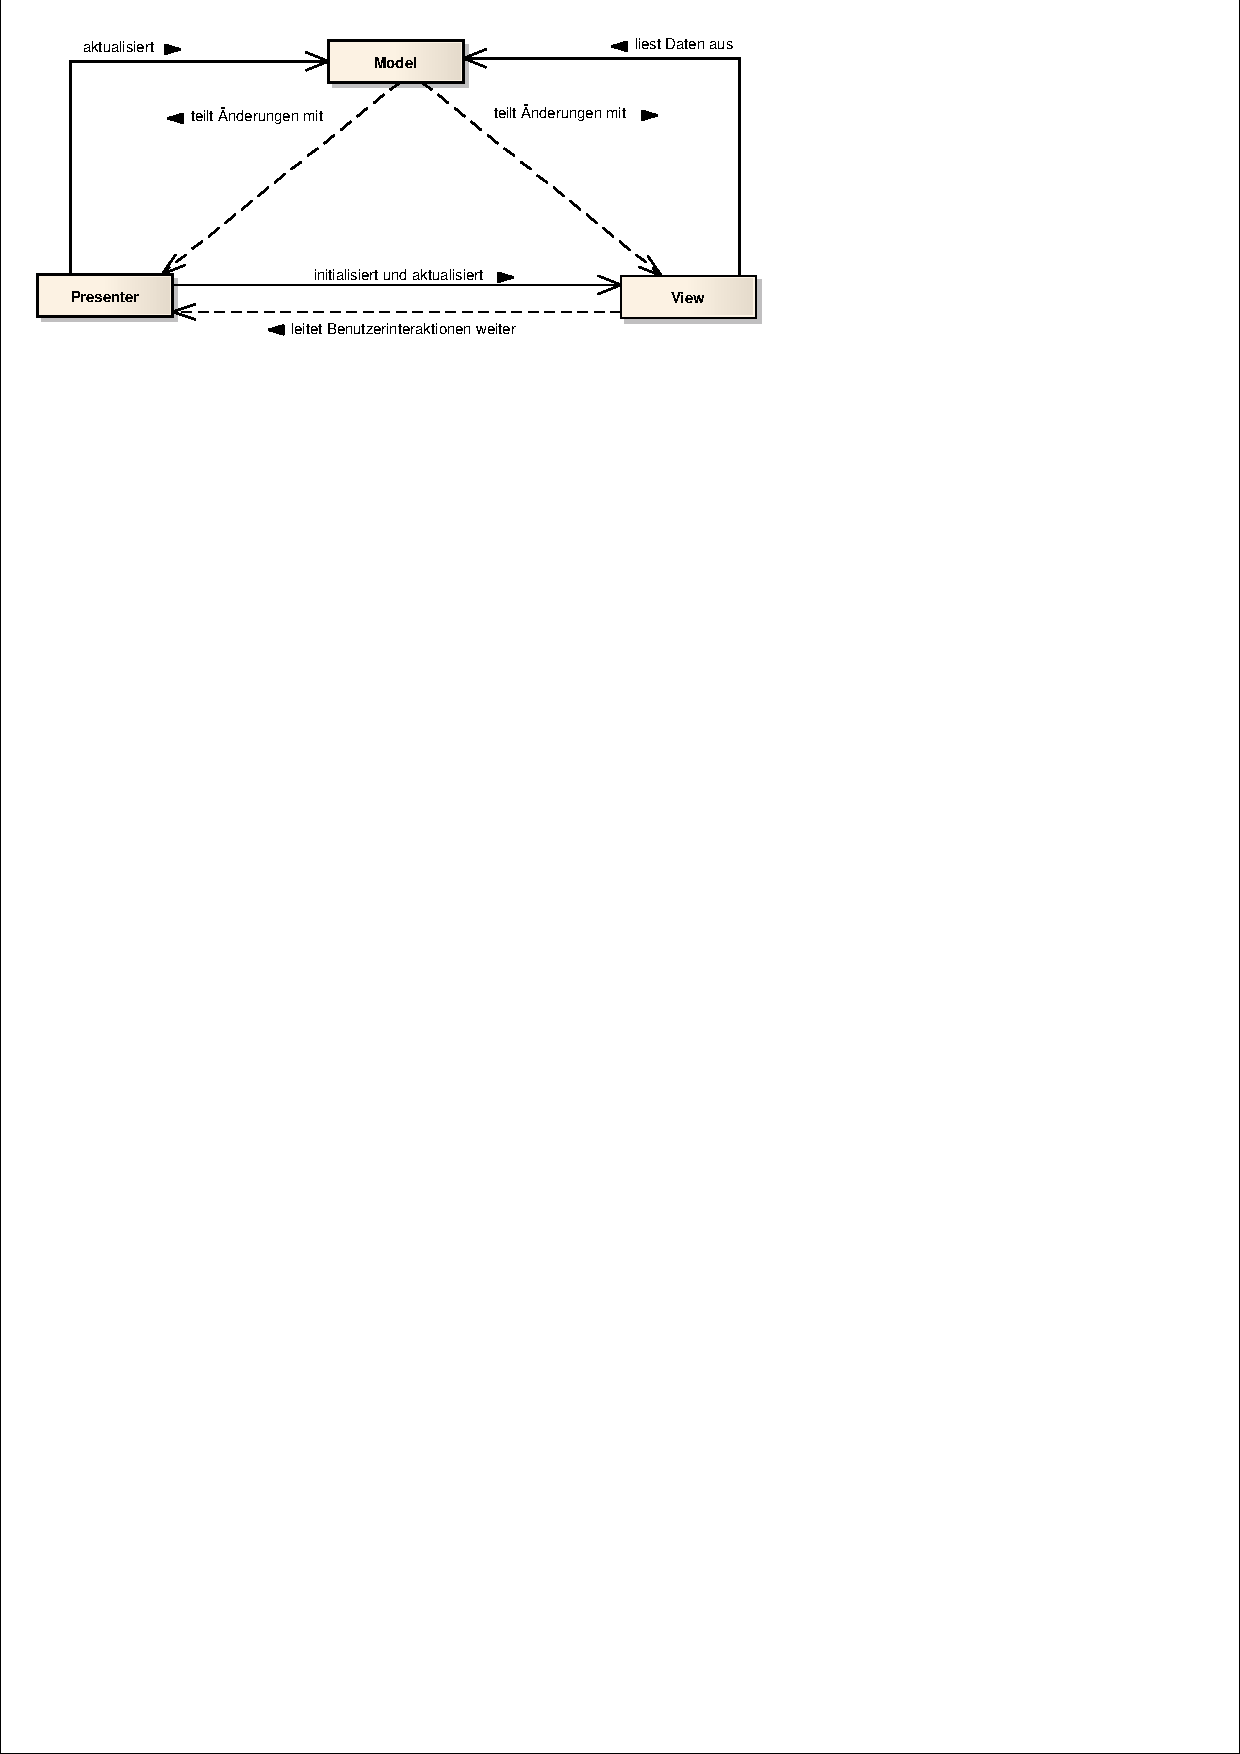
\includegraphics[trim = 2mm 238mm 80mm 2mm, clip, scale=0.7]{images/MVP.pdf}
\caption{�berblick �ber die \emph{Supervising Controllers} Variante des \emph{MVP Patterns}}\label{fig:mvp}
\end{figure}

Abbildung~\ref{fig:mvp} zeigt die \emph{Supervising Controllers} Variante des \emph{MVP Patterns} \cite{fowler}, welche vom \DevEnv\ verwendet wird. Jeder \emph{Presenter} hat genau eine \emph{View} und umgekehrt. Der \emph{Presenter} kennt seine \emph{View} und kann diese jederzeit aktualisieren und auf deren Daten zugreifen. Die \emph{View} hingegen kennt ihren \emph{Presenter} nicht. Um die Benutzereingaben dennoch an den \emph{Presenter} weiterleiten zu k�nnen, werden \emph{Events} verwendet. Der \emph{Presenter} reagiert darauf und aktualisiert gegebenenfalls die Daten des Modells. 

Die \emph{View} erh�lt ihre Daten entweder vollst�ndig vom \emph{Presenter}, oder kann diese aus dem Modell auslesen. �ndert sich das Modell, so werden die �nderungen �ber \emph{Events} sowohl an den \emph{Presenter} als auch an die \emph{View} geschickt. Im Regelfall bindet sich die \emph{View} per \emph{Databinding} an das Modell und wird so -- ohne zus�tzlichen Code -- automatisch aktualisiert, wenn sich das Modell �ndert. Der \emph{Presenter} kann ebenfalls auf �nderungen des Modells reagieren, um komplexere Pr�sentationslogik auszuf�hren und dann die \emph{View} zu aktualisieren. 

\section{System-Architektur}
In der ersten Iteration der Design-Phase wurde bereits die gesamte Architektur des \DevEnvs\ entworfen. Der erste Entwurf erwies sich als recht stabil und erforderte in sp�teren Iterationen nur wenige Modifikationen. Die erstellten Artefakte, ein Designmodell und mehrere Sequenzdiagramme, werden in den folgenden Abschnitten besprochen und die getroffenen Entscheidungen begr�ndet. Das Designklassen-Diagramm ist allerdings zu gro�, um es im Anhang dieser Arbeit abzubilden. Daher werden nur relevante Ausschnitte des Modells im Anhang beigelegt; das komplette Modell ist als .pdf-Datei auf der CD-ROM enthalten.

Da UML keine Syntax f�r .NET \emph{Properties} anbietet, wurde der Stereotyp \texttt{property} eingef�hrt. In der Implementierung wurden dann \texttt{Get/SetX}-Methoden mit \texttt{property}-Stereotyp als entsprechende \emph{Properties} \texttt{X \{ get; set; \}} umgesetzt. Aus Gr�nden der �bersichtlichkeit wurden im Designmodell f�r viele �ffentliche Attribute keine \emph{Properties} definiert; sie werden sp�ter aber als �ffentliche \emph{Properties} implementiert, da laut den .NET Richtlinien der Zugriff auf �ffentliche Klassenattribute immer durch \emph{Properties} gekapselt sein sollte \cite{fields}.

\subsection{\Horde-Klassen}
Die aus dem Konzeptmodell bekannten \Horde-Klassen wurden in das Designmodell �ber-nommen; alle Klassenattribute, die Assoziationen zwischen den Klassen und die Vererbungshierarchien sind unver�ndert. Es wurden allerdings mehrere Funktionen erg�nzt. So erh�lt die abstrakte Klasse \texttt{SceneNode} die virtuelle Methode \texttt{InitializeFromHorde3DState}, die aus dem aktuellen \Horde-Zustand beispielsweise die Transformationswerte und den Vaterknoten ausliest. Alle abgeleiteten Klassen k�nnen diese Methode �berschreiben, um ihre eigenen Daten auszulesen. Dabei k�nnen sie auf die \texttt{SceneNode}-Implementierung zur�ckgreifen, um die von \texttt{SceneNode} geerbten Attribute und Assoziationen zu f�llen beziehungsweise aufzubauen.

Ein analoges Vorgehen wurde f�r die Ressourcen-Hierarchie angewandt. Die abstrakte Klasse \texttt{Resource} besitzt ebenfalls eine virtuelle Methode \texttt{InitializeFromHorde3DState}, die in ihrer Standardimplementierung die \texttt{Resource}-Attribute und -Assoziationen ausliest und von den Subklassen �berschrieben werden sollte. Die Klasse \texttt{EditableResource} f�hrt zwei weitere abstrakte Methoden ein: \texttt{SaveToDisk} und \texttt{LoadFromDisk}. Konkrete Subklassen m�ssen diese Funktionen so implementieren, dass ihre Attribute und Assoziationen in das \Horde-XML-Format �bersetzt werden, beziehungsweise aus diesem ausgelesen und aufgebaut werden. Jedoch k�nnen manche Assoziationen nur dynamisch aus dem aktuellen \Horde-Zustand ermittelt werden, da sie in den XML-Dateien nicht gespeichert sind.

\subsection{Client-Server-Schnittstelle}
Wie bereits in Abschnitt~\ref{decisions} ausgef�hrt, zerf�llt das System in einen Client- und einen Serverteil. Da in der Design-Phase bereits die Windows Communication Foundation (WCF) als Netzwerk-Framework ausgew�hlt wurde, orientiert sich das Design der Client-Server-Schnittstelle an der Terminologie und an den F�higkeiten von WCF. 

Abbildung~\ref{fig:clientServerInterfaceDesign} zeigt einen Ausschnitt aus dem Designmodell f�r die Client-Server-Schnitt-stelle. Zun�chst wurde das Interface \texttt{IDebuggerService} spezifiziert, �ber das der Client auf den Server zugreifen kann. Der Service hat je eine Funktion f�r jede Systemanforderung: \texttt{Suspend} und \texttt{Resume}, um die Anwendung anzuhalten und wieder fortzusetzen; \texttt{Profile}, um die Profiling-Daten zu generieren; \texttt{GetRenderTargetData}, um den Inhalt eines \emph{Render Targets} auszulesen; und \texttt{UpdateResource}, um aktualisierte Ressource-Daten zu �bermitteln und an \Horde\ weiterzureichen.

Urspr�nglich lieferten die Funktionen bereits die jeweilig ben�tigten Daten zur�ck. %, was jedoch zu Deadlocks und Inkonsistenzen bei der Implementierung f�hrte\footnote{Die Deadlocks konnten entstehen, wenn w�hrend einer WCF-Operation weitere Benutzereingaben bearbeitet wurden. Da die WCF-Aufrufe sowohl client- als auch serverseitig immer in einem speziellen Thread stattfinden m�ssen.}. 
In der zweiten Iteration wurde hingegen das \texttt{IDebuggerServiceCallback}-Interface eingef�hrt. Der Server verwendet dieses Interface, um dem Client Daten und Ereignisse zu �bermitteln. Das \emph{Callback}-Interface vereinfachte das Einfrieren, Fortsetzen und Profilen der Anwendung aus der Anwendung selbst heraus. Wenn der Benutzer eine bestimmte Taste innerhalb der Anwendung dr�ckt, schickt der Server per \emph{Callback} eine Meldung an den Client, und dieser kann darauf entsprechend reagieren. Ohne \emph{Callbacks} w�re das in Sequenzdiagramm~\ref{fig:ClientServerCommunication} gezeigte Vorgehen nicht umsetzbar gewesen. Dort werden die \emph{Service}- und \emph{Callback}-Interaktionen beim Anhalten der Anwendung gezeigt. Der Client erh�lt vom Benutzer den Befehl zum Anhalten der Anwendung und ruft den \emph{Service} auf, welcher wiederum den Server informiert. Alternativ erteilt der Benutzer den Befehl durch einen Tastendruck innerhalb Anwendung direkt an den Server. In beiden F�llen ruft der Server die \texttt{OnSuspended}-Methode des \emph{Callbacks} auf. Eine Implementierung des \emph{Callback}-Interfaces w�rde den Client beispielsweise durch Ausl�sen eines \emph{Events} dar�ber informieren, dass die Anwendung angehalten wurde; der Client geht bis zu diesem Zeitpunkt in beiden F�llen immer noch davon aus, dass die Anwendung noch l�uft. Kam der \texttt{Suspend}-Aufruf direkt vom Server, so kann der Client davon nichts wissen. Kam der Aufruf hingegen vom Client selbst, so wurde er nur an den Server weitergereicht, aber sonst nicht darauf reagiert. Dadurch kann der Client unabh�ngig vom Ursprung des \texttt{Suspend}-Befehls die gleichen Aktionen durchf�hren. 

Erst wenn der Client durch den \emph{Callback} �ber das Einfrieren der Anwendung informiert wurde, fordert er mit der \texttt{RequestDebugData}-Methode des \emph{Services} die aktuellen Szenen\-graph- und Ressourcendaten an. Der Server schickt dann jede \emph{Scene Node} und jede Ressource einzeln �ber das \emph{Callback} Interface an den Client, der mit den Objekten entsprechend weiterarbeitet. Beim Fortsetzen oder Profilen der Anwendung w�re das Verfahren analog, es w�rden nur andere beziehungsweise gar keine Daten per \emph{Callback} an den Client zur�ckgeschickt werden. Eine Ausnahme bildet hingegen das Auslesen des Inhalts eines \emph{Render Targets}. Da die Anfrage ausschlie�lich vom Client kommen kann, bringt das \emph{Callback}-Verfahren hier keine Vorteile. Aus diesem Grund liefert die Funktion \texttt{GetRenderTargetData} das Ergebnis direkt zur�ck.

Ein weiterer Vorteil des \emph{Callback}-Interfaces ist die M�glichkeit, generierte \Horde-Mel\-dungen unverz�glich an den Client schicken zu k�nnen. Dies erspart ein kontinuierliches Nachfragen des Clients beim Server, ob neue Nachrichten erstellt wurden. Zus�tzlich werden alle \emph{Scene Nodes}, Ressourcen, \Horde-Meldungen und Profiling-Objekte einzeln �bertragen, was bei gro�en Datenmengen die Reaktionszeit des Clients verbessert. Statt auf die �bertragung des gesamten Datensatzes warten zu m�ssen, kann der Client nach und nach jedes Objekt, das er bereits erhalten hat, einzeln darstellen. 

Problematisch an der Einf�hrung des \emph{Callback}-Interfaces war hingegen, dass es prinzipiell m�glich sein k�nnte, dass \emph{Callbacks} vor dem Verbindungsaufbau aufgerufen werden. Aus diesem Grund stellt die Implementierung einen Sicherungsmechanismus bereit, der \emph{Callback}-Aufrufe abf�ngt und erst dann an den Client �bermittelt, wenn die Verbindung aufgebaut wurde.

Auf der Clientseite kennt nur die Klasse \texttt{Horde3DApplication} eine Instanz der Klasse \texttt{DebuggerServiceProxy}, �ber die der Client mit dem Server kommunizieren kann. Dabei repr�sentiert \texttt{Horde3DApplication} wie bereits im Konzeptmodell eine konkrete \Horde-Anwendung. Um eine Anwendung starten zu k�nnen, werden gewisse Informationen ben�tigt, wie der Pfad zur ausf�hrbaren Datei, die \emph{Endpoint}-Konfiguration f�r WCF, das Arbeitsverzeichnis etc. \texttt{Horde3DApplication} kennt diese Daten und die Methode \texttt{Start} startet eine neue Serverinstanz. Sobald der Server l�uft, dient die Klasse als Fassade f�r den Service \emph{Proxy}. Zum Beenden des Servers muss die Methode \texttt{ShutDown} aufgerufen werden.

\subsection{Umsetzung des DLL-Replacements und des Profilings}
Der gew�hlte DLL-\emph{Replacement}-Mechanismus macht die Einf�hrung von \emph{Proxy}-Funktionen erforderlich. Wenn die Anwendung eine \Horde-Funktion aufruft, so wird nicht sofort der Code der originalen \Horde\ DLL ausgef�hrt, sondern eine \emph{Proxy}-Funktion. Diese ruft die urspr�ngliche Funktion auf, f�hrt aber auch noch zus�tzlichen Code aus. Dieser Code h�ngt jedoch davon ab, ob der Server gerade die \Horde-Funktionsaufrufe f�r die Profiling-Funktion protokolliert. 

Um mit den unterschiedlichen Codepfaden zurechtzukommen, wurden die in Abbildung~\ref{fig:proxyDesign} gezeigte Klassenstruktur entworfen. \texttt{Horde3DProxyBase} ist eine abstrakte Basisklasse, die f�r jede \Horde-Funktion einen Funktionszeiger sowie eine gleichnamige, abstrakte Methode mit gleichen R�ckgabe- und Parametertypen wie die \Horde-Funktion besitzt. Aus Gr�nden der �bersichtlichkeit sind im Klassendiagramm~\ref{fig:proxyDesign} nur der Funktionszeiger und die \emph{Proxy}-Funktion f�r \texttt{Horde3D::getVersionString} eingezeichnet.

Die beiden Klassen \texttt{Horde3DNoProfilingProxy} und \texttt{Horde3DProfilingProxy} spezialisieren \texttt{Horde3DProxyBase}. Alle Funktionszeiger der Basisklasse werden geerbt und durch die ebenfalls geerbte \texttt{Initialize}-Methode initialisiert. Die beiden \emph{Proxy}-Klassen �berschreiben die abstrakten \Horde-Methoden: Es wird jeweils die urspr�ngliche \Horde-Funktion sowie die entsprechende Methode der statischen \texttt{Horde3DCall}-Klasse aufgerufen und gegebenenfalls die Profiling-Daten protokolliert. \texttt{Horde3DCall} besitzt f�r jede \Horde-Funktion eine statischen Methode und ein statisches \emph{Event}, welche jeweils die an die Funktion �ber\-ge\-benen Parameter und deren R�ckgabewert als Parameter erhalten. Wird eine \Horde-Methode der \texttt{Horde3DCall}-Klasse aufgerufen, so wird das entsprechende spezifische \emph{Event} sowie die beiden generischen \emph{Events} \texttt{Before-/AfterFunctionCalled}  ausgel�st, wobei letztere jeweils vor -- respektive nach -- dem Ausl�sen des speziellen Ereignisses ausgel�st werden. Objekte des Servers k�nnen sich an diesen \emph{Events} registrieren und werden somit informiert, wann und mit welchen Parameter- und R�ckgabewerten eine \Horde-Funktion aufgerufen wurde.

Die \texttt{Horde3DProxyHandler}-Klasse verwaltet die zwei verschiedenen \emph{Proxies} und h�lt eine Referenz auf die originale \Horde\ DLL, mit der die Funktionszeiger auf die \Horde-Funktionen ermittelt werden k�nnen. Mit \texttt{Initialize} werden die beiden \emph{Proxy}-Klassen initialisiert und eine Instanz des \texttt{Horde3DNoProfilingProxy} als Wert der \texttt{CurrentProxy}-Assoziation gesetzt. Die Methode \texttt{EnableProfiling} (de)aktiviert den Profiling-Modus, indem die \texttt{CurrentProxy}-Assoziation auf den entsprechenden \emph{Proxy} gesetzt wird.

Die API von \Horde\ verwendet allerdings keine Klassen, sondern organisiert die Funktionen im Namensraum \texttt{Horde3D}. Die \emph{Replacement}-DLL ben�tigt daher neben dieser Klassenstruktur noch \emph{Proxy}-Funktionen f�r alle \Horde-Funktionen im Namensraum \texttt{Horde3D} und eine globale Instanz der \texttt{Horde3DProxyHandler}-Klasse. Die \emph{Proxy}-Funktionen k�nnen dann mit der \texttt{GetCurrentProxy}-Methode der \texttt{Horde3DProxyHandler}-Klasse auf den derzeitigen \emph{Proxy} zugreifen und die entsprechende \Horde-Methode des \emph{Proxies} aufrufen. Dieser Vorgang wird am Beispiel des Profiling-\emph{Proxies} f�r die \Horde-Funktion \texttt{getVersionString} in Abbildung~\ref{fig:proxySeq} gezeigt, wobei zus�tzlich noch \texttt{FunctionCall}-Objekte f�r die Profiling-Funktionalit�t erzeugt werden.

Das beschriebene Design wurde gew�hlt, weil es eine klare Trennung zwischen den beiden verschiedenen \emph{Proxies} erm�glicht. Die Trennung wurde n�tig, da der Profiling-\emph{Proxy} f�r jeden Funktionsaufruf einige zus�tzliche Schritte durchf�hren und mehrere Objekte anlegen muss, was einen negativen Einfluss auf die Performance in CPU-limitierten Szenen hatte. Daher sollte der Profiling-Code, wenn er nicht ben�tigt wird, auch nicht ausgef�hrt werden. 

Es h�tte zwei denkbare Alternativen zur umgesetzten L�sung gegeben:

\begin{itemize}
	\item Man h�tte direkt in den \emph{Proxy}-Funktionen im \texttt{Horde3D}-Namensraum die Original-Funktionen aufrufen und den zus�tzlichen Code ausf�hren k�nnen, wobei man per \texttt{if-then-else} den Profiling-Code ein- und ausgeschaltet h�tte. Dadurch h�tte man sich den Aufruf der \texttt{GetCurrentProxy}-Methode gespart -- der aber im Regelfall vom Compiler sowieso \emph{inline} kompiliert wird -- und den virtuellen \Horde-Methodenaufruf des \emph{Proxies} durch die Auswertung einer Bedingung ersetzt. Der Performancevorteil der \texttt{if-then-else}-L�sung, falls �berhaupt messbar, w�re aber im Vergleich zur Aus\-f�hr\-ungs\-dauer der eigentlichen Funktionen so gering, dass statt dieser L�sung die im objekt-orientierten Sinne bessere Alternative gew�hlt wurde.
	
	\item Eine weitere Variante betrifft die \texttt{Horde3DCall}-Klasse. Diese bietet neben den beiden generischen \emph{Events}, die nur den Namen der aufgerufenen Funktion �bergeben, ein spezielles Ereignis mit Ein- und Ausgabewerten f�r jede \Horde-Funktion. Dies erfordert viel Code, der durch die Beschr�nkung auf die generischen \emph{Events} vermieden werden k�nnte. Dann m�sste man allerdings die Ein- und Ausgabewerte der aufgerufenen Funktionen als \texttt{Object}-\emph{Array} �bergeben. Das f�hrt aber bei jedem Funktionsaufruf zur Erzeugung vieler tempor�rer Objekte, erfordert \emph{Boxing} und \emph{Unboxing} f�r Parameter primitiver Datentypen und beim Zugriff auf das Parameter-\emph{Array} eine �berpr�fung der \emph{Array}-Grenzen sowie des Parametertyps. Da diese L�sung unperformant, belastend f�r den \emph{Garbage Collector} und zudem nicht einmal typsicher ist, wurde die aufw�ndigere, aber elegantere Variante gew�hlt.
\end{itemize}

\subsection{Anhalten der Anwendung}
In der ersten Iteration der Design-Phase war nicht klar, wie das Anhalten der Anwendung technisch genau l�sbar ist. Es wurde daher das \emph{Strategy Pattern} verwendet, um verschiedene Ans�tze m�glichst einfach ausprobieren und austauschen zu k�nnen. Abbildung~\ref{fig:suspendStrategyDesign} zeigt den relevanten Ausschnitt des Designmodells. Das Interface \texttt{ISuspendApplicationStrategy} stellt die beiden Funktionen \texttt{Suspend} und \texttt{Resume} bereit, nach deren Ausf�hrung die Anwendung entweder angehalten ist oder weiterl�uft. Bei der Implementierung zeigte sich, dass insgesamt drei verschiedene Strategien zum Anhalten der Anwendung ben�tigt werden: \texttt{StopTimeSuspendStrategy}, um der Anwendung ein Anhalten der Zeit vort�uschen zu k�nnen; \texttt{CursorSuspendStrategy}, um der Anwendung die Kontrolle �ber den Mauszeiger gezielt entziehen und wieder zur�ckgeben zu k�nnen; und \texttt{WndProcSuspendStrategy}, um das \emph{Window Procedure} der Anwendung ersetzen und damit Benutzereingaben �ber Maus und Tastatur abfangen zu k�nnen. Die Umsetzung dieser Strategien und ihre Probleme werden in Kapitel~\ref{suspendApp} genauer erl�utert.

Um diese Objekte nicht einzeln verwalten zu m�ssen, wurde in einer sp�teren Iteration die Container-Klasse \texttt{SuspendApplicationStrategy} hinzugef�gt, die ebenfalls vom \emph{Suspend}-Interface erbt. Einzige Aufgabe dieser Klasse ist es, beim Aufruf ihrer \texttt{Suspend}- und \texttt{Resume}-Methoden die entsprechenden Methoden aller Objekte im \texttt{Strategies}-\emph{Property} aufzurufen. In Kapitel~\ref{Ausblick} findet sich ein Vorschlag, wie man aufbauend auf dieser Instanz des \emph{Strategy Patterns} und der \texttt{SuspendApplicationStrategy}-Klasse eine weitere Strategie zum Anhalten der Anwendung integrieren k�nnte.

\subsection{Starten und Beenden des Servers}
Die Abbildungen~\ref{fig:startSeq} und~\ref{fig:DebuggerInitSeq} zeigen, was beim Starten des Servers nach Aufruf der \texttt{Start}-Methode der \texttt{Horde3DApplication}-Klasse geschieht. Zun�chst muss die originale \Horde\ DLL im Anwendungsverzeichnis umbenannt werden. Dann werden die ben�tigten DLLs des \DevEnvs\ in das Anwendungsverzeichnis kopiert, einschlie�lich der modifizierten \Horde\ DLL mit den \emph{Proxy}-Funktionen. Anschlie�end wird die Konfigurationsdatei f�r den Server generiert, die ebenfalls in das Anwendungsverzeichnis kopiert wird. Dannach wird der Prozess gestartet. Da es in der modifizierten \Horde\ DLL eine globale \texttt{Horde3DProxyHandler}-Variable gibt, wird beim Starten der Anwendung und nach dem Laden der modifizierten DLL automatisch eine \emph{Proxy Handler}-Instanz erzeugt. Der Konstruktor ruft die \texttt{Initialize}-Methode auf, die wiederum zun�chst den \texttt{Horde3DDebugger}-\emph{Singleton} initialisiert. Clientseitig wird sofort eine Instanz des \texttt{DebuggerServiceProxy} erzeugt und mit dem Verbindungsaufbau zum Server begonnen. Da es keine M�glichkeit gibt, vom Server �ber den Abschluss der Initialisierung informiert zu werden, wird einfach so lange ein Verbindungsaufbau versucht, bis der Serverprozess hochgefahren und initialisiert ist und die Verbindung erfolgreich aufgebaut werden konnte.

Auf der Serverseite werden Instanzen der beiden \Horde-\emph{Proxies} erzeugt und der Pro\-fil\-ing-Modus standardm��ig deaktiviert. Die Initialisierungsroutine des \texttt{Horde3DDebugger}-\emph{Single\-tons} liest zun�chst die Konfigurationsdaten aus der \emph{Settings}-Datei ein und �berpr�ft die \Horde-Version. Der gew�hlte DLL-\emph{Replacement}-Mechanismus macht es erforderlich, dass die Anwendung und der Server die gleiche Version von \Horde\ verwenden. Sollte das nicht der Fall sein, wird sich die Anwendung in vielen F�llen mit einer Windows-Fehler\-mel\-dung "`Prozedureinsprungspunkt "`\textit{ProzedurName}"' wurde in der DLL "`\Horde.dll"' nicht gefunden."' beenden, bevor der Server initialisiert wird. Es gibt aber auch F�lle, in denen Windows die fehlenden oder zus�tzlichen Einsprungspunkte nicht entdeckt. Dann �berpr�ft der Server anhand der \Horde-Versionskennung beider DLLs, ob unterschiedliche Versionen vorliegen. Sind die Versionen unterschiedlich, wird die Anwendung mit einer Fehlermeldung beendet.

Der \texttt{Horde3DDebugger}-\emph{Singleton} erzeugt neben der \texttt{DebuggerService}-Instanz noch zwei weitere Objekte: \texttt{Horde3DMessagesHandler} und \texttt{Horde3DStateWatcher}. Die Aufgabe des \texttt{Horde3DMessagesHandler}s ist es, nach jedem Funktionsaufruf eventuell neu generierten Meldungen abzufangen. Wurde eine oder mehrere Meldungen generiert, so werden die Daten ausgelesen, f�r jede neu generierte Nachricht ein \texttt{Horde3DMessage}-Objekt erzeugt und dieses per \emph{Callback} an den Client gesendet. 

Zu beachten ist hierbei die Phase der Initialisierung und Deinitialisierung des Servers. Der \texttt{Horde3DMessagesHandler} darf nur nach neuen Meldungen fragen, solange \Horde\ korrekt initialisiert ist. Wird beispielsweise \texttt{Horde3D::getVersionString} vor dem Aufruf von \texttt{Horde3D::init} aufgerufen, w�rde ohne korrekte \Horde-Initialisierung bereits nach dem Aufruf von \texttt{Horde3D::getVersionString} nach neuen Nachrichten gefragt. Auch nach dem Aufruf von \texttt{Horde3D::release} w�rde nach neuen Meldungen gefragt werden; zu diesem Zeitpunkt ist \Horde\ allerdings bereits vollst�ndig deinitialisiert. In beiden F�llen k�nnte es zu einem Absturz des Programms kommen.

Es ist allerdings kein Problem, wenn bereits Meldungen erzeugt werden, bevor der Client die Verbindung zum Server aufgebaut hat. Alle \emph{Callback}-Aufrufe werden abgefangen und erst ausgef�hrt, wenn die Verbindung steht.

Die \texttt{Horde3DStateWatcher}-Klasse hat derzeit nur die Aufgabe, unerw�nschtes \emph{Reverse-Engineering} zu unterbinden. Die Klasse k�nnte aber in Zukunft erweitert werden, um beispielsweise die Kamera, mit der die Szene gezeichnet wurde, zu protokollieren. Das k�nnte in Szenen mit mehreren Kameras und mehreren Aufrufen von \texttt{Horde3D::render} wichtig sein. Momentan �berpr�ft die Klasse allerdings nur, ob vor dem Aufruf von \texttt{Horde3D::render} die \Horde-Funktion \texttt{checkExtension} mit dem Parameter \texttt{AllowDebugging} aufgerufen wurde. Ist dies nicht der Fall, so wird beim Versuch die Szene zu zeichnen eine Fehlermeldung angezeigt und der Server beendet.

Das Beenden des Servers ist im wesentlichen eine Umkehr des Startprozesses. Die \texttt{ShutDown}-Methode der \texttt{Horde3DApplication}-Klasse schlie�t zun�chst die Verbindung zum Server und beendet den Prozess durch Schlie�en des Hauptfensters. Falls der Prozess nach einem kurzen \emph{Timeout} von wenigen Sekunden nicht beendet wurde, wird er zwangsweise terminiert. Anschie�end wird der urspr�ngliche Zustand des Anwendungsverzeichnis wiederhergestellt. Die in das Verzeichnis kopierten DLLs des \DevEnvs\ werden gel�scht und auch die erstellte Konfigurationsdatei wird entfernt. Zum Schluss wird der umbenannten, originalen \Horde\ DLL wieder ihr urspr�nglicher Name gegeben.

\subsection{Aktualisieren von Ressourcen-Daten}
Das Sequenzdiagramm~\ref{fig:UpdateResourceSeq} stellt das Vorgehen f�r die Aktualisierung von ge�nderten Ressourcen dar. Der Vorgang wird �ber die \texttt{Horde3DApplication}-Klasse angesto�en, da nur diese Klasse die \texttt{UpdateResource}-Operation des Servers aufrufen kann. Der Server f�hrt die interne \texttt{UpdateHorde3D}-Methode der �bergebenen \texttt{EditableResource} aus. Diese Methode ist virtuell und kann somit von den Subklassen �berschrieben werden. Das Sequenzdiagramm zeigt die Funktionsweise der Stand\-ard\-implementierung. Zun�chst wird �berpr�ft, ob die Ressource, die \Horde\ gerade unter dem gleichen \texttt{ResHandle} kennt, den gleichen Typ und gleichen Namen hat. Implizit wird damit auch �berpr�ft, ob �berhaupt noch eine Ressource mit diesem \texttt{ResHandle} existiert. Dies ist notwendig, weil es das \DevEnv\ erlaubt, die Anwendung nach dem Einfrieren der Szene und nach dem Auslesen der bekannten Ressourcen weiter auszuf�hren. Der Benutzer k�nnte nun eine Ressource bearbeitet haben und diese an die \texttt{UpdateResource}-Operation des Servers �bergeben. Zwischenzeitlich k�nnte die Anwendung die Ressource aber gel�scht und ihren \texttt{ResHandle} neu vergeben haben. Durch die �berpr�fung des Ressourcennamens und -typs soll verhindert werden, dass die �bergebene Ressource eine eventuell neu hinzugef�gte Ressource �berschreibt. Ansonsten w�rde die derzeit geladene Ressource durch eine eventuell v�llig andere ersetzt. Bei unterschiedlichen Typen w�rde \Horde\ eine Fehlermeldung erzeugen, da die �bergebenen Ressourcen-Daten dann nicht korrekt interpretiert werden k�nnen.

Ist die �berpr�fung jedoch erfolgreich, werden die derzeit geladenen Ressourcen-Daten gel�scht. Die Ressource selbst bleibt aber erhalten, insbesondere �ndert sich ihr \texttt{ResHandle} nicht. Nun k�nnen die Daten aus der �bergebenen \texttt{EditableResource} in ein \texttt{byte}-\emph{Array} kopiert und an \Horde\ �bergeben werden. Anschlie�end werden alle zur Zeit nicht geladenen aber bekannten Ressourcen geladen. Das ist erforderlich, weil die aktualisierte Ressource auf neue, noch nicht geladene Ressourcen verweisen k�nnte. Bevor die Szene mit der aktualisierten Ressource gezeichnet werden kann, m�ssen diese Abh�ngigkeiten geladen werden.

Wie bereits erw�hnt ist die \texttt{UpdateHorde3D}-Methode der \texttt{EditableResource}-Klasse virtuell. Werden n�mlich Shader- oder Material-Ressourcen aktualisiert, m�ssen noch einige zus�tzliche Schritte ausgef�hrt werden. \Horde\ erlaubt das Klonen von Materials, das hei�t, die Material-Ressource wird kopiert und der Kopie ein neuer \texttt{ResHandle} zugewiesen. Dadurch k�nnen zum Beispiel die \emph{Uniform}-Parameter des Materials f�r verschiedene Objekte unterschiedlich gesetzt werden. Allerdings werden die Kopien nicht aktualisiert, wenn das Original-Material aktualisiert wird. �bergibt man also eine \texttt{MaterialResource} an \texttt{UpdateResource}, so m�ssen alle Kopien des Materials gesucht und aktualisiert werden. Die Kopien sind an ihrem Namen erkennbar: hie� das Original-Material \texttt{Material1.material.xml}, dann hei�en die Klone \texttt{Material1.material.xml|X}, wobei $X$ der \texttt{ResHandle} der Kopie ist.

Wird eine \texttt{ShaderResource} an \texttt{UpdateResource} �bergeben, m�ssen ebenfalls noch weitere Ressourcen aktualisiert werden. Der GLSL-Code des Shaders wird von \Horde\ in zus�tzlichen Code-Ressourcen gespeichert. Wird ein Shader aktualisiert, werden allerdings die Code-Ressourcen nicht automatisch neu geladen. Dies muss manuell geschehen. Dazu werden die abh�ngigen Code-Ressourcen �ber den Namen ermittelt, der als Pr�fix den Namen der zugeh�rigen Shader-Ressource enth�lt. Allerdings kann diese Sonderbehandlung der Shader-Ressourcen f�r zuk�nftigen \Horde-Versionen entfallen. Alle Versionen nach \Horde\ 1.0.0 Beta 3 aktualisieren automatisch auch alle abh�ngigen Code-Ressourcen.
\section{Anbindung der Benutzeroberfl�che an das System}
Die Anbindung der grafischen Benutzeroberfl�che an den Anwendungscode wurde bislang nicht weiter betrachtet, ist jedoch ein komplexes Problem. F�r das \DevEnv\ wurde eine eigene Bibliothek entwickelt, die die GUI-Anbindung an das System kapselt und einige Grundfunktionalit�ten bereitstellt. Dabei standen die Wiederverwendbarkeit der Bibliothek sowie eine saubere Trennung zwischen GUI- und Anwendungscode im Vordergrund. 

\subsection{Alternativen zur Eigenentwicklung eines GUI-Frameworks}
Bevor mit der Entwicklung eines eigenen GUI-Frameworks begonnen wurde, wurden zwei alternative Ans�tze in Betracht gezogen: Die Integration des Clients in Visual Studio oder in SharpDevelop\footnote{\url{http://www.icsharpcode.net/OpenSource/SD}} als Plugin. Beide Tools haben eine ausgereifte, m�chtige und bew�hrte Plugin-Architektur und bieten viele Schnittstellen zu Subsystemen -- wie einen Texteditor mit \emph{Syntaxhighlighting}, eine Konsole f�r Textausgabe, ein \emph{Undo}/\emph{Redo}-Framework, ein Framework zum automatischen Speichern ge�nderter Dateien, etc. --, die das \DevEnv\ ebenfalls ben�tigt. Es bestand also ein gro�es Potential, bereits vorhandene und erwiesenerma�en gut funktionierende L�sungen wiederzuverwenden. Dennoch wurde auf diesen Vorteil verzichtet, da die Nachteile �berwogen. Visual Studio ist ein extrem komplexes und im Kern auch sehr altes System, das zu weiten Teilen noch in \C++ und COM implementiert ist. Plugins k�nnen zwar in \Csharp/.NET entwickelt werden, allerdings sind die Interfaces, die Visual Studio bereitstellt, aufgrund ihres Alters �berladen, schwer verst�ndlich und nicht mehr zeitgem��. Au�erdem muss ein Plugin nach jeder �nderung neu integriert werden, was die Entwicklung verz�gert und ein schnelles Debuggen unm�glich macht. Ein weiteres Problem ist, dass nicht jeder potenzielle Benutzer des \DevEnvs\ eine Visual Studio Lizenz besitzt; die kostenlosen Express-Versionen unterst�tzen leider keine Plugins. Die eigenst�ndig lauff�hige Visual Studio Shell w�rde diese Probleme zwar l�sen, w�re aber aufgrund ihrer Gr��e (ca. 150 MByte) und Komplexit�t eine sehr belastende Abh�ngigkeit f�r das \DevEnv.

SharpDevelop hingegen wurde von Anfang an komplett in \Csharp\ entwickelt und ist Open Source. Die Einbindung von Plugins gestaltet sich angenehmer als unter Visual Studio und es gibt moderne objekt-orientierte APIs f�r den Zugriff auf die Standardkomponenten der Entwicklungsumgebung. Leider ist die Entwicklung von Plugins f�r SharpDevelop sehr schlecht dokumentiert. Es gibt zwar einf�hrende Erl�uterungen, aber eine prototypische Implementierung des \DevEnvs\ zeigte schnell, dass bei komplexeren Fragen und Problemen oft keine Hilfestellung in der Dokumentation, im Internet oder im inzwischen veralteten Buch \cite{sharpdevelop} existiert. Da die IDE Open Source ist, konnte die Antwort zwar immer durch Durchsehen des Quellcodes gefunden werden, dies nahm aber sehr viel Zeit in Anspruch. Visual Studio hingegen ist teilweise deutlich besser dokumentiert. Aber auch hier gibt es noch einige Defizite, insbesondere bei der Erweiterung der Standard-Projektverwaltung mit dem \emph{Visual Studio Managed Package Framework for Projects}\footnote{\url{http://www.codeplex.com/mpfproj}}.

\subsection{Architektur des GUI-Frameworks}\label{sec:aufbau}
Um eine klare Trennung zwischen GUI- und Anwendungscode zu erreichen, ist das GUI-Framework eine Instanz des \emph{Model-View-Presenter Patterns}. Es wurde au�erdem von Anfang an auf die Entwicklung einer Visual Studio-�hnlichen Oberfl�che ausgelegt, kann aber prinzipiell auch f�r andere UI-Designs verwendet werden. 

Abbildung~\ref{fig:guiClass} zeigt das Designklassen-Diagramm des GUI-Frameworks. Die Verwendung des \emph{Model-View-Presenter Patterns} wird durch die abstrakte Klasse \texttt{Presenter} und das Interface \texttt{IView} deutlich. Im GUI-Framework selbst kommen keine Modelle vor; diese sind anwendungsspezifisch und werden von den Applikationen, die das Framework verwenden, bereitgestellt.

Es gibt insgesamt vier Klassen, die das \texttt{IView}-Interface implementieren. Diese Klassen ergeben sich aus dem Design moderner GUI-Frameworks wie Windows Forms und der Windows Presentation Foundation. Dort gibt es zum einen \texttt{Form}-Klassen, welche ein eigenst�ndiges Fenster repr�sentieren. Diesen Fenstern k�nnen mehrere Instanzen von \texttt{UserControl}-Klassen untergeordnet sein, beispielsweise f�r Eingabefelder oder Schaltkn�pfe. Um das Visual Studio-�hnliche Design zu realisieren, gibt es noch eine weitere spezielle Klasse, \texttt{DockContent}, deren Instanzen ebenfalls einer \texttt{Form} untergeordnet sein m�ssen. Dabei kann eine \texttt{DockContent}-Instanz sowohl ein eventuell verstecktes \emph{Dock Pane} an der Seite der Oberfl�che, ein \emph{Floating Window} oder ein Dokument sein. F�r all diese Klassen wird eine \texttt{IView}-Implementierung ben�tigt. \texttt{UserControlView} erbt von \texttt{UserControl} und \texttt{FormView} ist von \texttt{Form} abgeleitet, wobei hier zwischen modalen und nicht-modalen Fenstern unterschieden wird. \texttt{DockView} erbt von \texttt{DockContent} und f�gt zwei Attribute hinzu, um den standardm��igen \texttt{DockState} und die Menge der erlaubten \texttt{DockState}s festzulegen. \texttt{DocumentView} ist eine Subklasse von \texttt{DockView}, wobei hier der standardm��ige \texttt{DockState} und die Menge der erlaubten \texttt{DockState}s fest auf \texttt{Document} beschr�nkt sind.

Die abstrakte Klasse \texttt{Presenter} ist die Basisklasse f�r alle \emph{Presenter} im System. Instanzen von \texttt{Presenter} werden �ber einen Namen identifiziert; f�r einen gegebenen Namen kann es immer nur eine \texttt{Presenter}-Instanz geben. \texttt{Presenter} hat eine private Assoziation zu einem \texttt{IView}, auf die abgeleitete Klassen nur �ber die Funktion \texttt{UpdateView} zugreifen k�nnen. Damit wird zum einen die Kopplung zur \emph{View} verringert und zum anderen m�ssen in dieser Funktion noch einige implementierungsspezifische Details (Zugriff �ber korrekten Thread, kein Zugriff auf bereits gel�schte \emph{Views}, etc.) geregelt werden. Zu beachten ist, dass nur die abstrakte \texttt{Presenter}-Klasse ihre zugeh�rige \emph{View} kennt; insbesondere kennen die \texttt{IView}-Instanzen nicht ihre zugeh�rige \texttt{Presenter}-Instanzen. Dies wird durch das \texttt{Request}-Ereignis, das alle \texttt{IView}-Implementierungen besitzen, erm�glicht. Ein \emph{Presenter} registriert sich an den \texttt{Request}-Ereignissen seiner \emph{View} und kann dar�ber �ber Eingaben und Aktionen des Benutzers informiert werden.

Die GUI-\emph{Controls} bilden eine Hierarchie aus \texttt{Form}-, \texttt{DockContent}- und \texttt{UserControl}-In\-stan\-zen. Diese Hierarchie m�ssen auch die \emph{Presenter} widerspiegeln. Aus diesem Grund kann ein \texttt{Presenter} einen \texttt{Parent} und beliebig viele \texttt{Children} haben, die �ber die Funktionen \texttt{Add-/RemoveChildPresenter} hinzugef�gt und wieder entfernt werden k�nnen. \texttt{Presenter} hat au�erdem abstrakte Methoden f�r die Initialisierung und Deinitialisierung. Abgeleitete \texttt{Presenter}-Klassen m�ssen diese Methoden mit einer speziellen Implementierung �ber\-schrei\-ben. Die \emph{Presenter}- und \emph{View}-Hierarchien  sind eine Instanz des \emph{Composite Patterns}.

Da eine \emph{Undo}/\emph{Redo}-Funktionalit�t ben�tigt wird, werden vom Benutzer ausgef�hrte Aktionen gem�� des \emph{Command Patterns} durch Objekte gekapselt, die von der abstrakten Klasse \texttt{Command} erben m�ssen. Ein \texttt{Command} hat Funktionen zum Ausf�hren der Aktion (\texttt{Execute}), sowie zum R�ckg�ngigmachen (\texttt{Undo}) und Wiederholen (\texttt{Redo}); wobei \texttt{Redo} standardm��ig einfach noch einmal \texttt{Execute} aufruft und \texttt{Execute} und \texttt{Undo} abstrakt sind. Es ist auch m�glich, die \emph{Undo}/\emph{Redo}-Funktionalit�t f�r einen \texttt{Command} zu deaktivieren, indem die \texttt{CanUndo}- und \texttt{CanRedo}-Attribute auf \texttt{false} gesetzt werden. Instanzen von \texttt{Command} werden immer von einem \texttt{Presenter} erzeugt und jeder \texttt{Command} kennt seinen Erzeuger. �ber diese Assoziation k�nnen alle \texttt{Command}-Objekte eines \texttt{Presenter}s beim Entfernen des \texttt{Presenter}s aus der GUI gel�scht werden, wodurch die Aktionen dieser \texttt{Command}s nicht mehr r�ckg�ngig gemacht werden k�nnen.

\texttt{Command}-Objekte werden vom \texttt{CommandDispatcher} verwaltet. Dessen \texttt{HandleCommand}-Me-thode ruft die \texttt{Execute}-Methode des �bergebenen \texttt{Command}s auf und verwaltet intern eine \emph{Undo}-/\emph{Redo}-Liste von bereits ausgef�hrten Aktionen. Der \texttt{CommandDispatcher} kann �ber die Funktionen \texttt{Undo} und \texttt{Redo} angewiesen werden, eine Aktion r�ckg�ngig zu machen oder zu wiederholen. Dies ist allerdings nur m�glich, wenn das \texttt{CanUndo}- respektive das \texttt{CanRedo}-Attribut des \texttt{CommandDispatcher}s auf \texttt{true} gesetzt ist. �ndert sich der Wert eines dieser Attribute wird ein entsprechendes Ereignis ausgel�st, ebenso nach dem R�ckg�ngigmachen und Wiederholen einer Aktion.

Das \DevEnv\ stellt editierbare Ressourcen als \texttt{DocumentView}-Instanzen dar. Nach dem �ndern einer Ressource sollen die �nderungen gespeichert werden k�nnen. Au�erdem soll das Framework einen visuellen Hinweis geben, falls ein Dokument ge�ndert wurde, aber die �nderungen noch nicht gespeichert sind. Schlie�t der Benutzer ein ge�ndertes und noch nicht gespeichertes Dokument, so soll das Framework den Benutzer fragen, ob die �nderungen gespeichert oder verworfen werden sollen. Diese Aufgaben �bernimmt die \texttt{SaveableContentManager}-Klasse, an der \texttt{Presenter}, die das \texttt{ISaveableContentPresenter}-Interface implementieren, registriert und wieder entfernt werden k�nnen. Registrierte \texttt{ISaveableContentPresenter}-Instanzen k�nnen einzeln oder alle auf einmal gespeichert werden. Wird ein ge�nderter, aber noch nicht gespeicherter \texttt{Presenter} geschlossen, so wird der Benutzer gebeten, die �nderungen zu speichern oder zu verwerfen.

Das \texttt{ISaveableContentPresenter}-Interface stellt Methoden zum Laden und Speichern des zu persistierenden Objekts bereit. Auch der aktuelle \texttt{SaveState} wird dort verwaltet. Das Interface wird von der abstrakten Klasse \texttt{SaveableContentPresenter} implementiert, die die normale \texttt{Presenter}-Klasse erweitert.

Die \texttt{Shell}-Klasse ist schlie�lich das Hauptelement des Frameworks. In ihr laufen alle Vorg�nge zusammen. \texttt{CommandDispatcher} und \texttt{SaveableContentManager} sind mit einer 1:1-Assoziation zur \texttt{Shell} verbunden und h�tten somit auch direkt in die \texttt{Shell}-Klasse integriert werden k�nnen. Dies h�tte jedoch zu einer niedrigen Koh�sion und damit zu einer �berladung der \texttt{Shell}-Klasse gef�hrt, was durch die Verteilung der Zust�ndigkeiten vermieden wurde. Da der \texttt{SaveableContentManager} nur der \texttt{Shell} bekannt ist, ist die \texttt{Shell} hier eine Instanz des \emph{Facade Patterns}. Auch das \emph{Singleton Pattern} wird von der \texttt{Shell} verwendet: Mit dem \texttt{Current}-Attribut kann global auf die \texttt{Shell}-Instanz zugegriffen werden, wobei es nur eine \texttt{Shell}-Instanz pro \emph{AppDomain} geben darf. Dies ist konsistent mit dem Vorgehen der \texttt{Application}-Klasse der Windows Presentation Foundation.

Die Aufgabe der \texttt{Shell}-Klasse ist neben der Initialisierung der gesamten Oberfl�che auch die Verwaltung aller \texttt{Presenter}-Instanzen. \texttt{Presenter} k�nnen hinzugef�gt, wieder entfernt und Dokumente einzeln oder gemeinsam gespeichert oder geschlossen werden. Auch das Layout der \emph{Dock Panes} wird von der \texttt{Shell}-Klasse automatisch persistiert und beim Starten der Anwendung wiederhergestellt.

\subsection{Identifizierung der ben�tigten Modelle}
Modelle tauchen in Abbildung~\ref{fig:guiClass} nicht auf, da das GUI-Framework kein Interface und keine Zugriffswege f�r Modelle vorgibt. Dies erm�glicht einem \emph{Presenter}-\emph{View}-Paar die Verwendung mehrere Modelle, wovon die Implementierung des \DevEnvs\ auch Gebrauch macht. Insgesamt werden zur Umsetzung der Systemanforderungen sechs Modelle ben�tigt, die im Designmodell mit dem Stereotyp \texttt{model} gekennzeichnet sind.

\begin{itemize}
	\item \texttt{\textbf{Horde3DApplication}}: Die \texttt{Horde3DApplication}-Klasse repr�sentiert die \Horde-An-wendung, in der gerade der Server l�uft oder die gestartet werden kann. Sie ist die einzige Zugriffsm�glichkeit auf Operationen des Servers.
	
	\item \texttt{\textbf{CallbackHandler}}: Der \texttt{CallbackHandler} nimmt die \emph{Callbacks} des Servers entgegen und generiert f�r jede Nachricht ein entsprechendes \emph{Event}. Die \emph{Presenter} k�nnen sich an der \texttt{CallbackHandler}-Instanz an verschiedenen Ereignissen registrieren, um �ber Server-Nachrichten informiert zu werden.
	
	\item \texttt{\textbf{MessagesDispatcher}}: Die Aufgabe des \texttt{MessagesDispatcher}-Modells ist die Verwaltung aller erzeugten Nachrichten. Die Nachrichten k�nnen zum einen aus der \Horde-Anwendung stammen oder vom Client generierte Fehler- oder Debugmeldungen sein. Die Nachrichten werden nach ihrer Herkunft (Client oder Server) kategorisiert und nach Wichtigkeit (Debug, Information, Warnung oder Fehler) unterschieden. Der \emph{Dispatcher} unterst�tzt auch das Entfernen aller Nachrichten einer bestimmten Kategorie. Nachdem Meldungen entfernt oder hinzugef�gt wurden, wird ein spezielles Ereignis ausgel�st, damit die interessierten \emph{Presenter} und \emph{Views} entsprechend reagieren k�nnen.
	
	\item \texttt{\textbf{SceneGraph}} und \texttt{\textbf{ResourceGraph}}: Diese beiden Modelle dienen zum Verwalten aller bekannten \emph{Scene Nodes} und Ressourcen. Werden neue Objekte eingef�gt oder Objekte entfernt, wird ein \texttt{GraphChanged}-\emph{Event} ausgel�st, um die �nderungen bekannt zu machen.
	
	\item \texttt{\textbf{ProfilingDataManager}}: Dieses Modell funktioniert �hnlich der beiden zuvor genannten Modelle und verwaltet die Profiling-Daten. Das \texttt{ProfilingDataChanged}-\emph{Event} wird ausgel�st, wenn Profiling-Daten empfangen oder gel�scht werden.
\end{itemize}

\begin{figure}[htp]
\centering
%trim=l b r t  	This option will crop the imported image by l from the left, b from the bottom, r from the right, and t  from the top. Where l, b, r and t are lengths. 
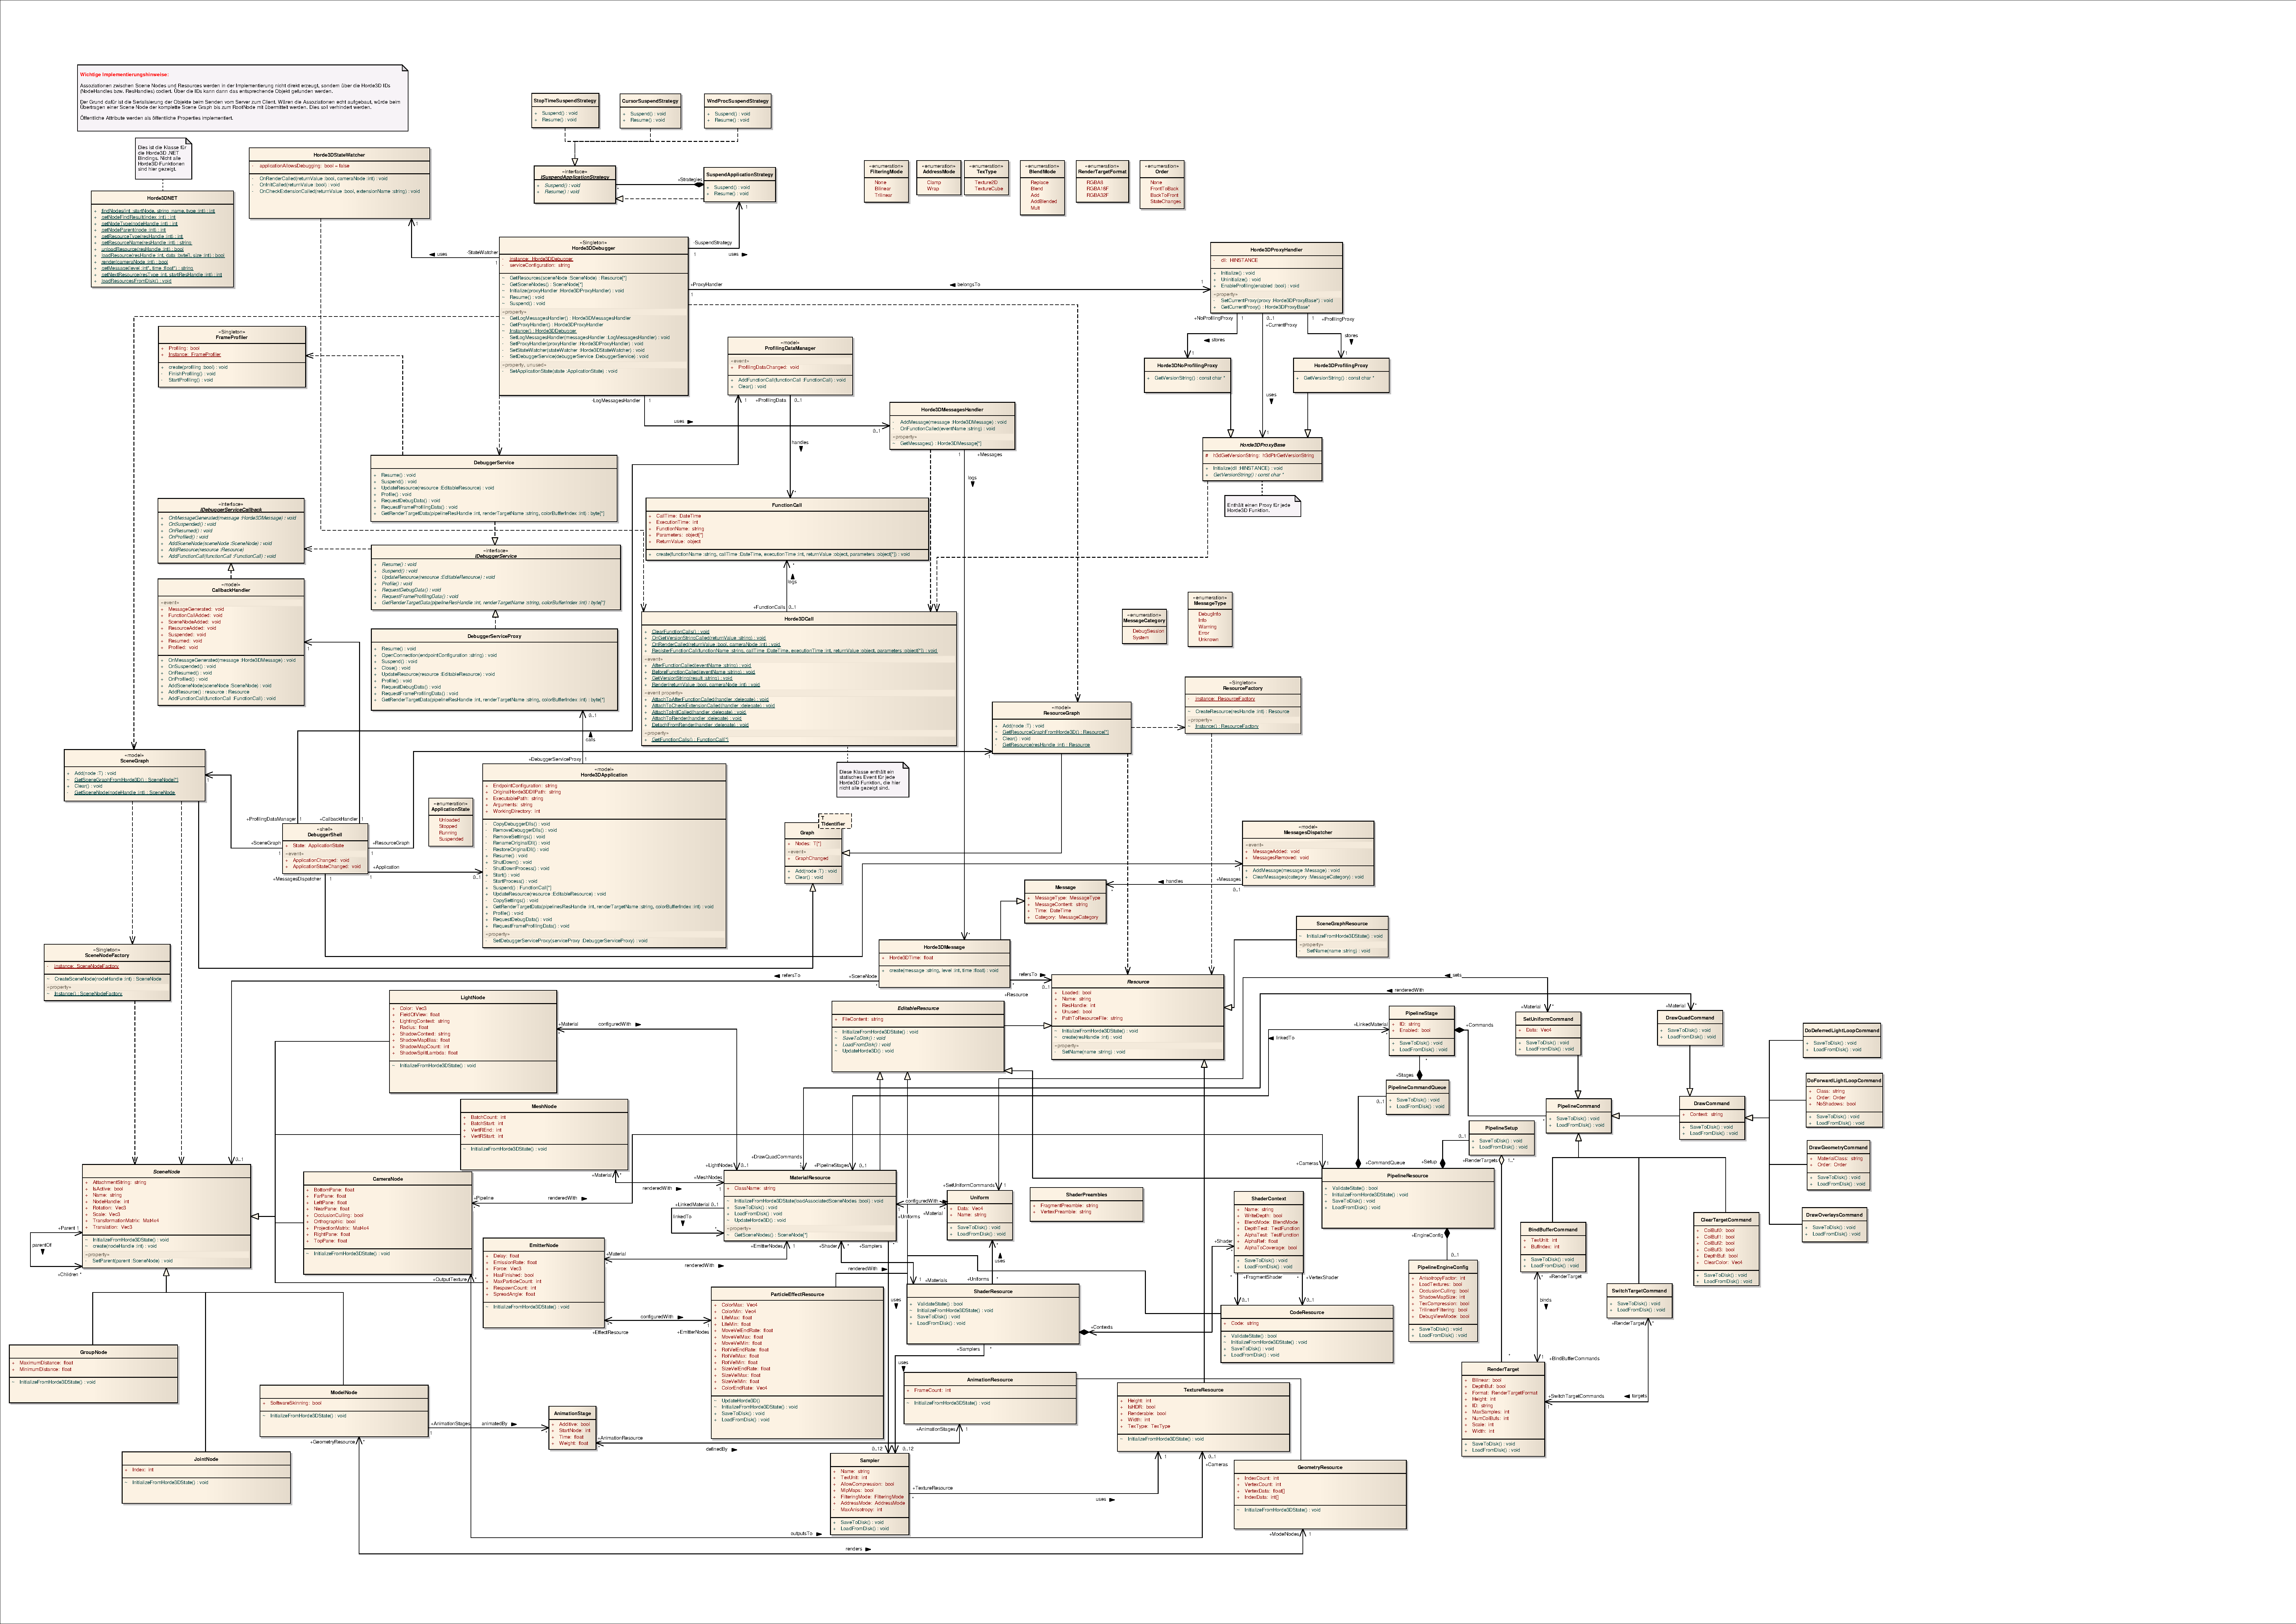
\includegraphics[trim = 125mm 380mm 975mm 415mm, clip, scale=0.7]{images/Designmodell.pdf}
\caption{Die Shell des \DevEnvs\ im Designmodell}\label{fig:shellDesign}
\end{figure}

Alle Modelle werden von der \texttt{Shell}-Klasse verwaltet, wodurch alle \emph{Presenter} Zugriff auf alle Modelle erhalten. Die \texttt{Shell}-Klasse �berwacht au�erdem den aktuellen Zustand des Servers, da einige \emph{Presenter} und \emph{Views} bei Zustands�nderungen spezielle Aktionen durchf�hren m�ssen. Die m�glichen Zust�nde sind \texttt{Unloaded}, wenn derzeit kein \texttt{Horde3DApplication}-Modell geladen ist und somit der Server nicht gestartet werden kann; \texttt{Stopped}, wenn der Server zur Zeit nicht l�uft aber gestartet werden kann; \texttt{Suspended}, wenn der Server gerade l�uft und die Szene eingefroren ist; und \texttt{Running} sonst. Die \texttt{Shell}-Klasse l�st ein \emph{Event} aus, sobald sich der Zustand des Servers �ndert.
\section{Konklusion}
In der Design-Phase wurden viele generische Konzepte verwendet, um flexibel auf m�gliche �nderungen von \Horde\ oder eventuell auftauchende Probleme in der Implementierungs-Phase reagieren zu k�nnen. Aufgrund der detaillierten Analyse der Anforderungen und dem Aufbau von \Horde\ konnte ein Systemdesign erstellt werden, das bei der Implementierung nur wenige Probleme verursachte. Die notwendigen �nderungen am Design beschr�nkten sich jedoch immer auf einzelne Klassen; die grundlegende Architektur blieb bestehen. Eine gr��ere �nderung ergab sich lediglich durch die Einf�hrung der Client-Server-\emph{Callbacks}. 

Im Rahmen dieser Bachelorarbeit wurde aber nicht das komplette Design implementiert. So gibt es gerade bei den \Horde-Klassen einige Attribute und Assoziationen, die zwar im Designmodell vorhanden sind, f�r die Umsetzung der Systemanforderungen aber nicht erforderlich waren. Sie wurden dennoch in das Konzept- und Designmodell aufgenommen, um die Modelle zu vervollst�ndigen. Im Code k�nnen diese bei Bedarf einfach hinzugef�gt werden.

Bei der Entwicklung des \DevEnvs\ wurde auch deutlich, dass der verwendete DLL-\emph{Replacement}-Mechanismus sowie die Einf�hrung der \texttt{Horde3DCall}-Klasse richtige Entscheidungen waren. Insbesondere die beiden Klassen \texttt{Horde3DMessagesHandler} und \texttt{Horde3DStateWatcher} zeigten, warum das Ausl�sen von generischen als auch spezifischen Ereignissen mit den genauen Aufrufsparametern und R�ckgabewerten nach einem \Horde-Funktionsaufruf sinnvoll ist. Diese Informationen sind f�r unterschiedlichste Aktionen n�tzlich; so wurde beim Entwurf dieses Verfahrens nicht an die Verwendung eines \emph{Reverse-Engineering}-Schutzes gedacht. Sowohl die \texttt{Horde3DStateWatcher}-Klasse als auch die Anforderung vor dem Schutz vor unerw�nschtem \emph{Reverse-Engineering} wurden erst in einer sp�teren Iteration ins \DevEnv\ aufgenommen und f�gten sich nahtlos in das Systemdesign ein.

Die Entwicklung des GUI-Frameworks war zeitaufw�ndig und h�tte vermieden werden k�n\-nen, wenn das \DevEnv\ als Plugin f�r Visual Studio oder SharpDevelop entwickelt worden w�re. Aufgrund verschiedener Unzul�nglichkeiten der Plugin-Infrastruktur der IDEs hat sich die Eigenentwicklung schlie�lich doch als die bessere L�sung herausgestellt, da sich w�hrend der Implementierung des Systems die St�rken des Frameworks zeigten und ein z�gige und unkomplizierte Umsetzung des Designs erm�glichten. So ist der GUI- und Anwendungscode stets klar voneinander abgegrenzt und es ist einfach, neue Features durch Implementieren weiterer \texttt{Presenter}- und \texttt{View}-Klassen hinzuzuf�gen. Die Wiederverwendbarkeit und Erweiterbarkeit des Frameworks konnte bereits im Rahmen der Bachelorarbeit �berpr�ft werden. So wurde zu einem sp�teren Zeitpunkt eine weitere \texttt{DockView}-Subklasse, \texttt{WpfDockView}, hinzugef�gt, mit der Windows Presentation Foundation \texttt{UserControl}s in Windows Forms \texttt{DockView}s dargestellt werden k�nnen. Der Einsatz des Frameworks bei der Entwicklung des Code Generators, siehe Abschnitt~\ref{CodeGen}, best�tigte die Wiederverwendbarkeit der Bibliothek.

\chapter{Phase III: Implementierung}

Nach der ersten Iteration der Design-Phase war die grunds�tzliche Architektur und Funktionsweise des \DevEnvs\ festgelegt. In der Implementierungs-Phase wurde das Design in \C++/CLI und \Csharp\ mit Visual Studio 2008 Service Pack 1 umgesetzt. Es wurde eine Vielzahl an \emph{Third Party} Bibliotheken und Frameworks eingesetzt, um den Programmierungsaufwand m�glichst gering zu halten.

Zun�chst wurde mit der Umsetzung des DLL-\emph{Replacement}-Mechanismus begonnen, dann wurde das GUI-Framework implementiert. Anschlie�end wurden die einzelnen Systemanforderungen inkrementell programmiert. Durch das inkrementelle Vorgehen konnten schnell die ersten Features umgesetzt und getestet und dadurch auch fr�h m�gliche Designfehler entdeckt werden. Die Einf�hrung der \emph{Callbacks} wurde beispielsweise w�hrend der Umsetzung des Szenengraph-Explorers vorgenommen, bevor die erste Zeile f�r die Ressourcen oder die Profiling-Daten geschrieben worden war.

Da die wichtigsten Entscheidungen bereits w�hrend der Analyse- und Design-Phasen getroffen worden waren, konnte das Design z�gig umgesetzt werden. In den folgenden Abschnitten werden nun wichtige technische Details erl�utert, die in den vorherigen Phasen noch keine Rolle spielten. Dabei wird allerdings weitestgehend auf das Abdrucken von Code verzichtet und nur die verwendeten Konzepte erl�utert. Der komplette Source Code befindet sich auf der beiliegenden CD-ROM.

\section{Verwendete Technologien und Frameworks}
Zur Umsetzung des \DevEnvs\ wurde auf kommerzielle und frei verf�gbare Open Source Bibliotheken und Frameworks zur�ckgegriffen, um gewisse Standardl�sungen nicht selbst entwickeln zu m�ssen. Insbesondere basiert das System auf dem .NET Framework von Microsoft\footnote{\url{http://www.microsoft.com/NET}}.

\subsection{.NET Framework}
2002 ver�ffentliche Microsoft das .NET Framework, welches seither stark erweitert und verbessert wurde. �hnlich wie bei Java wird der Code zun�chst in eine Zwischensprache, die \emph{Common Intermediate Language}, �bersetzt und dann zur Laufzeit von der \emph{Common Language Runtime} (CLR) mit einem \emph{Just-in-Time-Compiler} in Maschineninstruktionen umgewandelt. Das .NET Framework spezifiziert ein vereinheitlichtes Typsystem, das \emph{Common Type System}, bietet die M�glichkeit f�r \emph{Reflection} und Code Generierung zur Laufzeit und verwendet einen \emph{Garbage Collector} zum Aufr�umen und Verwalten des Speichers. Inzwischen gibt es viele Sprachen, die in die \emph{Common Intermediate Language} �bersetzt werden k�nnen und somit Zugriff auf alle Klassen des .NET Frameworks besitzen. Die wichtigsten sind \Csharp, Visual Basic .NET und \C++/CLI \cite{dotnet}. 

Das Framework und \Csharp\ sind ECMA- und ISO-standardisiert. Es gibt verschiedene Implementierungen des Frameworks, wobei Microsoft offiziell nur Windows, mobile Ger�te wie Handys oder Zune und die XBOX 360 unterst�tzt. F�r Linux- und Mac-Systeme ist Mono\footnote{\url{http://www.mono-project.com/Main_Page}} weit verbreitet.

Das \DevEnv\ ist in \Csharp\ 3.0 und \C++/CLI implementiert. Es ist jedoch nur unter Windows lauff�hig, da sowohl der Client als auch der Server native, Windows-spezifische Funktionen und Bibliotheken verwenden. Dieser Nachteil wurde jedoch bewusst in Kauf genommen, da die Verwendung des .NET Frameworks und der plattform-abh�ngigen Bibliotheken eine einfachere und schnellere Implementierung erm�glichte.

Neben der \emph{Base Class Library}, die nur grundlegende Klassen wie Ein-/Ausgabestreams, Dateizugriffe, Strings, Listen, Hash-Tabellen und Warteschlangen anbietet, verwendet das \DevEnv\ vor allem auch Windows Forms (WinForms) f�r die Umsetzung der GUI, die Windows Communication Foundation (WCF) f�r die Interprozesskommunikation und Language Integrated Queries (Linq) f�r Filterung und Sortierung von Listen. Windows Forms basiert auf der mit Windows 95 eingef�hrten Win32-API und wurde mit dem Update auf .NET 3.0 durch die modernere Windows Presentation Foundation (WPF) abgel�st. Dennoch wird Windows Forms aufgrund seiner Einfachheit und hohen Effizienz -- sowohl bei der Entwicklung als auch beim Laufzeitverhalten -- gerne noch f�r Anwendungen eingesetzt, die keine speziellen Anforderungen, wie \emph{Themes} oder Animationen, an das grafische Design stellen. Da die GUI des \DevEnvs\ sich am Standard-Design von Windows orientiert, wurde WinForms als UI-Framework gew�hlt. Obwohl Mono vollst�ndig kompatibel zu Windows Forms ist \cite{winforms}, ist der Client nur unter Windows lauff�hig. Zur Umsetzung der GUI wurden zwei Bibliotheken verwendet, Weifen Luo Winforms Docking und das Krypton Toolkit, die native Win32-Funktionen aufrufen und somit von Mono unter Linux und Mac-OS nicht unterst�tzt werden k�nnen.

Die Windows Communication Foundation ist Microsofts Ansatz, eine einheitliche API f�r die plattformunabh�ngige, service-orientierte Netzwerkprogrammierung mit dem .NET Framework zu schaffen; insbesondere ersetzt WCF TCP-Sockets und das .NET Remoting. WCF kann sehr flexibel an die Anforderungen des Systems angepasst werden und ist somit sowohl f�r Webservices als auch f�r die Interprozesskommunikation geeignet. Da Client und Server des \DevEnvs\ auf dem gleichen Rechner laufen, werden \emph{Named Pipes} zur Kommunikation eingesetzt. Die Verwendung von \emph{Named Pipes} mit WCF garantiert eine performante, verl�ssliche und geordnete �bertragung der Nachrichten in einem Bin�rformat. \emph{Callback} Kontrakte werden ebenfalls unterst�tzt \cite{wcf}.

Linq wird durch eine Reihe neuer Klassen im .NET-Framework realisiert, deren Verwendung durch neue \Csharp\ 3.0-Sprachfeatures vereinfacht wird \cite{linq}. Es erlaubt auf eine deklarative Weise, Listen, XML-Dateien und Datenbanktabellen zu durchsuchen, zu sortieren und zu gruppieren. Diese Operationen sind in herk�mmlichen objekt-orientierten oder imperativen Sprachen oft mit viel Code verbunden; durch Linq wird der Code k�rzer und pr�ziser, wie man es von Datenbankanfragen mit SQL gew�hnt ist. Zusammen mit Linq verwendet das \DevEnv\ auch weitere neue Sprachfeatures von \Csharp\ 3.0, wie Extension-Methoden und Lambda-Funktionen. Mit Extension-Methoden kann man beliebige Klassen um Funktionen erweitern, ohne den Source Code der Klasse zu �ndern oder von ihr zu erben. Lambda-Funktionen bieten eine kurze Syntax zum Definieren anonymer Methoden. Das folgende Beispiel verdeutlicht diese Konzepte:

\lstset{language=Java} 
\begin{lstlisting}
// Diese Extension-Methode ruft auf jedem Element der Liste "source"
// die Funktion "func" auf.
public static void Foreach<T>(this List<T> source, Action<T> func)
{
	if (source == null)
		return;

	foreach (var item in source)
		func(item);
}

// Mit diesem Linq-Query werden alle Ressourcen, deren ResHandle 
// gr��er 10 ist, nach ihrem Namen sortiert ausgew�hlt.
var resources = from r in ResourceManager.Resources
								where r.ResHandle > 10
								order by r.Name
								select r;
								
// Anwendung der Extension-Methode "Foreach". Das Argument f�r 
// "source" ist "resources", das Argument f�r "func" ist eine
// Lambda-Funktion.
resources.Foreach(r => r.Reload());
\end{lstlisting}

\subsection{Verwendete Third Party Bibliotheken}

Die Implementierung des \DevEnvs\ verwendet die folgenden Bibliotheken, die alle kostenlos eingesetzt werden d�rfen. Sofern bekannt wurden die Lizenzen der Bibliotheken ebenfalls aufgelistet.

\begin{itemize}
	\item \textbf{Weifen Luo Winforms Docking} (\textit{MIT License})\footnote{\url{http://sourceforge.net/projects/dockpanelsuite}}: Die Bibliothek wird zur Umsetzung des Visual Studio \emph{User Interfaces} aus Abbildung~\ref{fig:vs} verwendet. Alle f�r die Umsetzung der GUI ben�tigten Features sind vorhanden; es wurden lediglich einige kosmetische Verbesserungen durchgef�hrt. Auch SharpDevelop verwendet diese Bibliothek.
	
	\item \textbf{Superlist} (\textit{Microsoft Permissive License v1.1})\footnote{\url{http://www.codeplex.com/Superlist}}: Dieses \emph{User Control} erweitert die \texttt{ListView}- und \texttt{Grid}-Klassen aus Windows Forms um einige neue Features und bietet eine einfachere Schnittstelle als die Standardklassen.
	
	\item \textbf{Krypton Toolkit} (\textit{kommerziell/kostenlos)}\footnote{\url{http://www.componentfactory.com}}: Das Toolkit ist Teil der kommerziellen Krypton Suite, darf aber frei verwendet werden. Es enth�lt Erweiterungen f�r viele WinForms-Standard-\emph{Controls}, um eine grafisch ansprechendere Oberfl�che zu erstellen.
	
	\item \textbf{Detours Express} (\textit{kommerziell/kostenlos})\footnote{\url{http://research.microsoft.com/en-us/projects/detours}}: Mit dieser Bibliothek von Microsoft Research k�nnen Aufrufe nativer Funktionen auf andere Funktionen umgeleitet werden. Allerdings werden in der Express-Version nur 32 Bit Prozesse unterst�tzt.
	
	\item \textbf{ExceptionReporter} (\textit{GNU Library General Public License})\footnote{\url{http://www.codeplex.com/ExceptionReporter}}: Tritt w�hrend der Aus\-f�hrung des Clients eine unerwartete Ausnahme auf, so zeigt der Exception Reporter einen Dialog mit einer ausf�hrlichen Fehlerbeschreibung an. Der Benutzer kann den Entwickler dann per Email �ber den aufgetretenen Fehler informieren.
	
	\item \textbf{SharpDevelop TextEditor} (\textit{GNU Library General Public License})\footnote{\url{http://www.icsharpcode.net/OpenSource/SD}}: Der Text Editor der SharpDevelop IDE unterst�tzt \emph{Syntaxhighlighting} f�r \Csharp, \C++/CLI und XML. %Das \DevEnv\ verwendet den Editor, um die XML-Dateien der Ressourcen anzuzeigen. Der Code Generator zeigt eine Vorschau des generierten \Csharp- und \C++-Codes einer \Horde-Funktion mit diesem Editor an.
	
	\item \textbf{ScalablePictureBox} (\textit{Open Source/unbekannt})\footnote{\url{http://www.codeproject.com/KB/miscctrl/ScalablePictureBox.aspx}}: %\emph{Render Targets} sind oft gr��er als das Fenster, in dem sie dargestellt werden. 
	Das \texttt{ScalablePictureBox}-\emph{Control} erlaubt es, ein dargestelltes Bild mit einem Klick zu verkleinern und wieder zu vergr��ern und den dargestellten Teil des Bildes zu verschieben.
	
	\item \textbf{Microsoft Chart Controls} (\textit{propriet�r/unbekannt})\footnote{\url{http://microsoft.com/downloads/details.aspx?FamilyId=130F7986-BF49-4FE5-9CA8-910AE6EA442C}}: Das .NET Framework enth�lt keine vorgefertigten APIs zum Darstellen von Diagrammen. Die Chart Controls Bibliothek von Microsoft f�llt diese L�cke und erm�glicht eine grafische Auswertung der Profiling-Daten im \DevEnv.
	
	\item \textbf{TGAReader} (\textit{The Code Project Open License})\footnote{\url{http://www.codeproject.com/KB/graphics/TargaImage.aspx}}: Die \texttt{Image}-Klasse des .NET Frameworks kann keine Bilder im .tga-Format laden. Die \texttt{TargaImage}-Klasse f�gt die .tga-Unterst�tzung hinzu.
	
	\item \textbf{Horde3D} (\textit{GNU Lesser General Public License})\footnote{\url{http://www.horde3d.org}}: Das \DevEnv\ verwendet die C- und \Csharp-Bindings von \Horde. Allerdings ist der Client nicht direkt von der DLL, sondern nur vom Aufbau und der Funktionsweise der Engine abh�ngig. Der Server hingegen ruft direkt Funktionen von \Horde\ auf.
\end{itemize}
\section{Implementierung des DLL-Replacement-Mechanismus}\label{CodeGen}
Die Klassenstruktur in Abbildung~\ref{fig:proxyDesign} zusammen mit der Klasse \texttt{Horde3DCall} bilden die Grundlage des DLL-\emph{Replacement}-Mechanismus. Die \emph{Proxy}-Klassen und der \emph{Handler} wurden in \C++/CLI geschrieben, \texttt{Horde3DCall} hingegen in \Csharp. Daher muss die DLL, die die originale \Horde\ DLL der Anwendung ersetzt, sowohl nativen Code als auch \emph{managed} Code enthalten. Die \emph{Proxy}-Funktionen im \texttt{Horde3D}-Namensraum sind nativer Code innerhalb der DLL und k�nnen daher von der unmodifizierten Anwendung ohne Neukompilierung -- also v�llig transparent -- aufgerufen werden. Diese nativen Funktionen wiederum rufen den \emph{Handler} auf, der \emph{managed} ist und somit vollen Zugriff auf alle �ffentlichen \Csharp-Klassen hat.

Problematisch ist die Menge des Codes, der f�r die Umsetzung des Designs erforderlich ist. \Horde\ 1.0.0 Beta 3 hat 78 �ffentliche Funktionen, f�r die jeweils folgender Code notwendig ist: Ein \emph{Delegate}-Typ, ein Ereignis und eine Funktion in \texttt{Horde3DCall}; ein Funktionszeiger und dessen Initialisierung sowie in eine virtuelle Funktion in \texttt{Horde3DProxyBase}; eine Implementierung der virtuellen Funktion in \texttt{HordeProfilingProxy} und \texttt{Horde3DNoProfilingProxy}; und eine native \emph{Proxy}-Funktion. In der derzeitigen Implementierung des \DevEnvs\ sind das rund 4800 Zeilen Code, die zun�chst geschrieben und dann f�r jede API-�nderung von \Horde\ von Hand angepasst werden m�ssten. Um diese un\-in\-te\-res\-sante und fehleranf�llige Arbeit zu vermeiden, wurde ein Code Generator entwickelt, der den kompletten Code des DLL-\emph{Replacement}-Mechanismus aus dem \Horde-\emph{Header} erzeugt.

\subsection{Code Generator Phase I: Analyse}
In der Analyse-Phase f�r den Code Generator wurde untersucht, wie das Tool arbeiten soll und was f�r Probleme bei der automatischen Typumwandlung von nativen \C++-Typen in .NET-Typen entstehen k�nnen. Die Typ-Konvertierungen wurden in folgende Kategorien eingeteilt:

\begin{itemize}
	\item Primitive Typen wie \texttt{int} und \texttt{float} k�nnen ohne manuelle Konvertierung sowohl in \emph{managed} als auch \emph{unmanaged} Code verwendet werden.
	\item Aufz�hlungstypen m�ssen �ber ihre \texttt{Integer}-Repr�sentation konvertiert werden.
	\item Die \texttt{NodeHandle}- und \texttt{ResHandle}-Datentypen von \Horde\ sind nur Umbenennungen von \texttt{int}. Da man in .NET aber keine globalen Typ-Aliase einf�hren kann, muss eine Konvertierung in \texttt{int} vorgenommen werden.
	\item \Horde\ verwendet \texttt{const char*} als String-Repr�sentation. �ber den Konstruktor der .NET \texttt{String}-Klasse k�nnen die \texttt{const char*}-\emph{Arrays} konvertiert werden.
	\item Im Gegensatz zu \texttt{const char*} sind alle anderen Zeiger problematisch. Es ist nicht klar, ob ein Zeiger einen \emph{out}-Parameter einer Funktion repr�sentiert oder ob er auf eine einzelne Variable oder auf ein ganzes \emph{Array} verweist. Daher kann bei einem Zeiger-Parameter oder -R�ckgabewert keine automatische Typumwandlung vorgenommen werden. 
\end{itemize}

Der Code Generator soll eine \Horde-\emph{Header}-Datei parsen und den n�tigen Code aus Abbildung~\ref{fig:proxyDesign} sowie die Klasse \texttt{Horde3DCall} generieren. Er soll eine mit dem GUI-Framework erstellte Oberfl�che bieten, die problematische Konvertierungen hervorhebt. Eine Konvertierung ist problematisch, wenn die Umwandlung in einen .NET-Typ nicht automatisch bestimmt werden kann, was im wesentlichen nur Zeiger betrifft. F�r Zeiger auf primitive Typen kann allerdings vermutet werden, dass sie \emph{out}-Parameter sind und entsprechend einfach nur dereferenziert werden m�ssen. Diese Standardkonvertierung f�r Zeiger auf primitive Typen muss aber als problematisch markiert werden, weil auch ein \emph{Array} des primitiven Typs gemeint sein k�nnte. V�llig unklar hingegen ist die Konvertierung von \texttt{void}-Zeigern.

Der Benutzer soll die M�glichkeit haben, eigenen Code zum Umwandeln des Typs anzugeben oder eine der oben aufgelisteten Standardkonvertierungen auszuw�hlen. Er soll au�erdem in der Lage sein, das Konvertierungsproblem als gel�st zu markieren. Alle manuellen �nderungen sollen aber bei der Neugenerierung des Code nach Updates der \Horde-API �bernommen werden k�nnen. Der Code Generator soll nur f�r die Generierung des Codes zust�ndig sein; die syntaktische Korrektheit des Codes, den der Benutzer eingegeben hat, muss nicht �berpr�ft werden. Der generierte Code soll f�r unproblematische Typumwandlungen sowohl syntaktisch als auch semantisch korrekt sein.

\begin{figure}[htp]
\centering
%trim=l b r t  	This option will crop the imported image by l from the left, b from the bottom, r from the right, and t  from the top. Where l, b, r and t are lengths. 
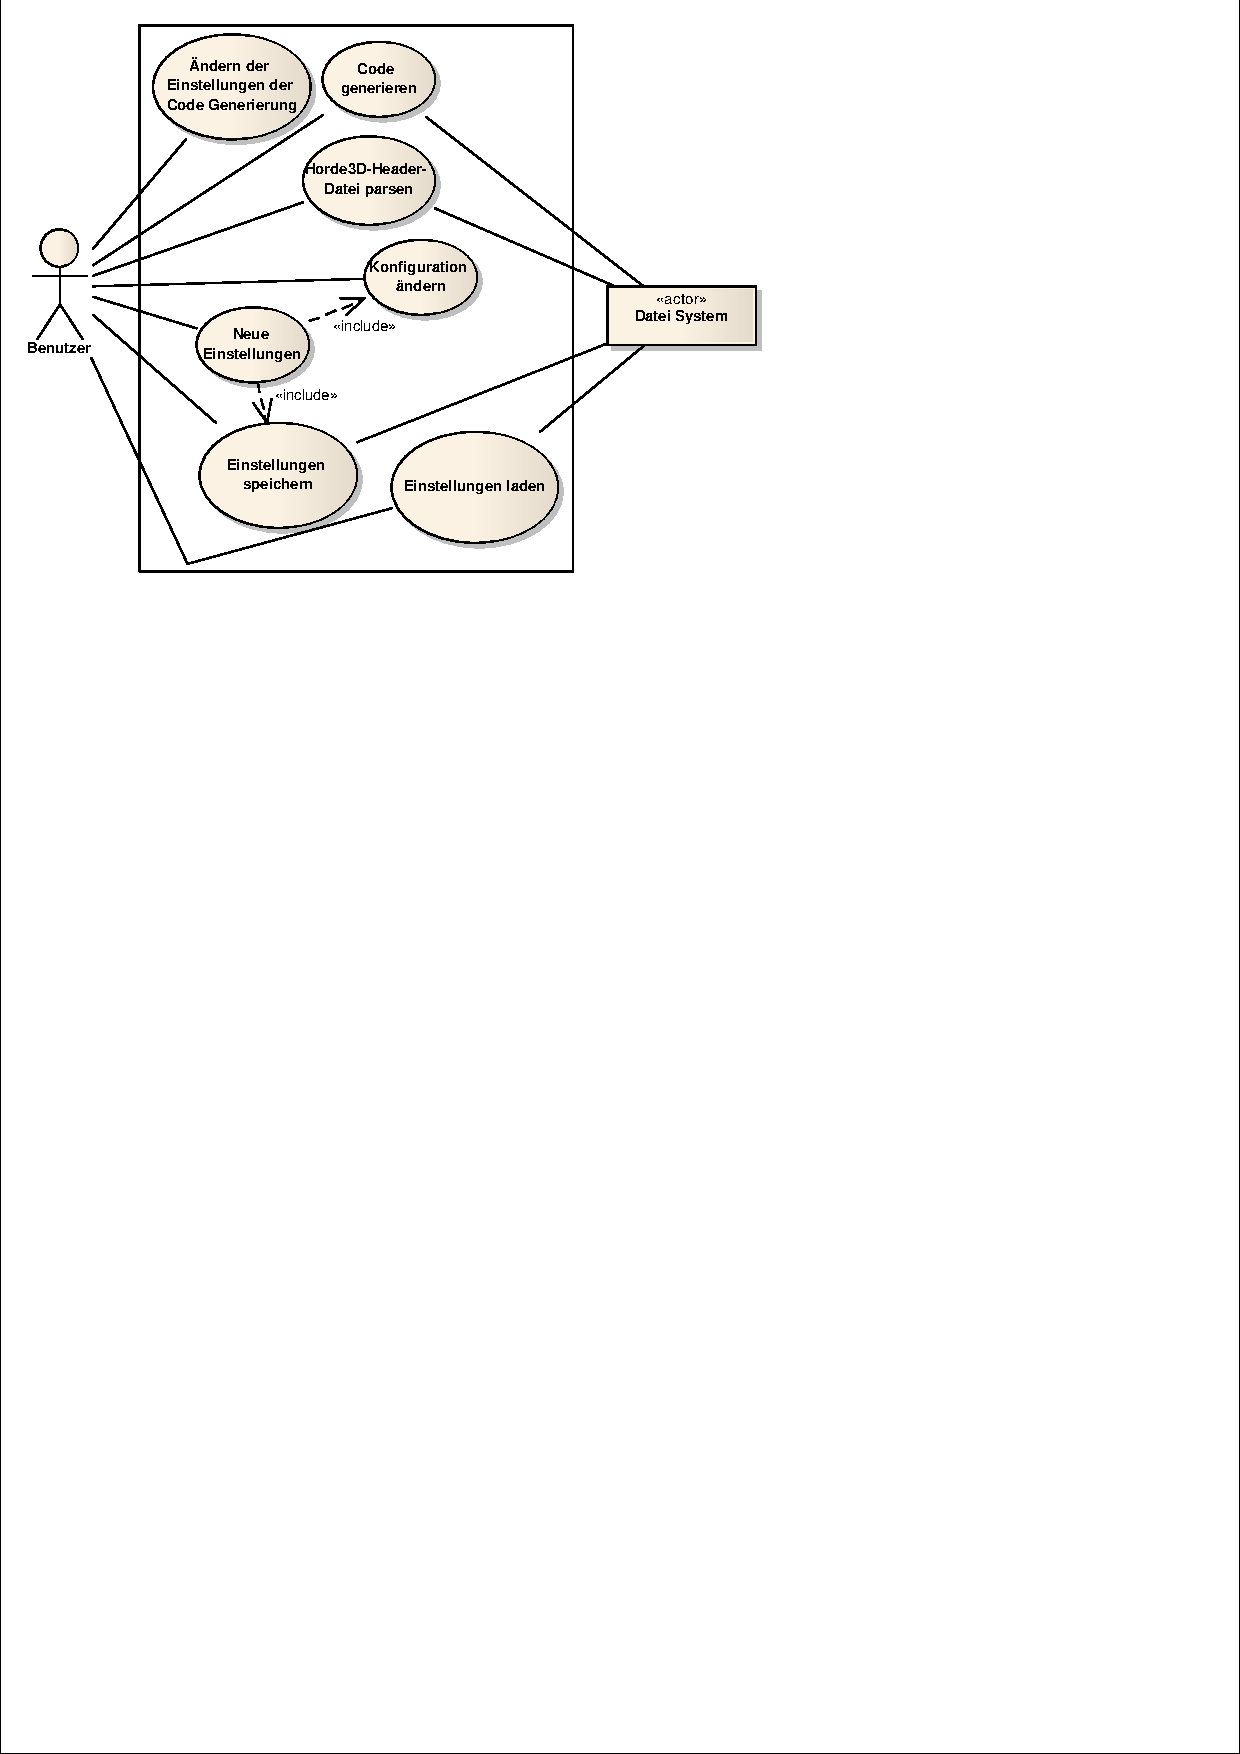
\includegraphics[trim = 1mm 200mm 80mm 1mm, clip, scale=0.7]{images/CodeGen_UseCaseModel.pdf}
\caption{Das \emph{Use Case} Modell des Code Generators}\label{fig:cgUCModel}
\end{figure}

Die im \emph{Use Case} Modell~\ref{fig:cgUCModel} gezeigten Anwendungsf�lle des Code Generators sind weitestgehend selbsterkl�rend. Mit dem System soll man die vorgenommenen Einstellungen speichern und sp�ter wieder laden k�nnen. Der Benutzer soll au�erdem den Namen der generierten Code-Dateien angeben k�nnen und auf Wunsch alle Einstellungen verwerfen und von vorne beginnen k�nnen. Interessanter sind die Anwendungsf�lle f�r das �ndern der Einstellungen der Code Generierung und f�r das Parsen der \emph{Header}-Datei. Ersteres wird durch das Aktivit�tsdiagramm~\ref{fig:cgChange} dargestellt. Wenn der Benutzer die Einstellungen �ndern m�chte, zeigt ihm das System zun�chst alle problematischen Funktionen an. In der Liste sind alle Funktionen, f�r die die Konvertierung mindestens eines Parameters oder des R�ckgabewertes problematisch ist. Auf Wunsch kann sich der Benutzer aber auch alle \Horde-Funktionen anzeigen lassen. Der Benutzer kann nun eine der Funktionen ausw�hlen, und das System zeigt die ausgew�hlten Typumwandlungen f�r alle Parameter und den R�ckgabetyp an. Problematische Konvertierungen werden hervorgehoben. Ein Konvertierungsproblem kann nun als gel�st markiert werden, oder die automatisch gew�hlte Umwandlung ge�ndert werden. Das System speichert die �nderungen, und der Benutzer kann weitere Einstellungen der gew�hlten Funktion oder weiterer Funktionen �ndern.

Beim Parsen der \emph{Header}-Datei von \Horde\ sollen alle Funktionen und ihre Parameter- und R�ckgabetypen ausgelesen werden. Es soll versucht werden, eine automatische Typumwandlung f�r alle Typen der Funktion zu finden. Gelingt dies nicht, soll die Umwandlung als problematisch markiert werden. Falls eine aktualisierte \emph{Header}-Datei geparst wird und der Benutzer vor dem Update bereits manuelle Einstellungen vorgenommen hat, sollen diese �bernommen werden. Es muss dazu f�r jede zuvor manuell ge�nderte Funktion �berpr�ft werden, ob die �nderungen auf die neu geparste Funktion �bertragen werden k�nnen. Sollte dies nicht gelingen, so soll die Funktion als problematisch markiert werden und die alten Einstellungen zus�tzlich zu den neu generierten gespeichert werden.

Abbildung~\ref{fig:cgDomain} zeigt das Konzeptmodell des Code Generators. \texttt{CodeGenerationSettings} speichert den Dateinamen der zu generierenden \C++- und \Csharp-Dateien, sowie eine Liste der \Horde-Funktionen. Die Einstellungen k�nnen in einer Datei gespeichert und wieder geladen werden. Der programmiersprachliche Aufbau der Funktionen wurden in seine Bestandteile zerlegt: Das \texttt{Function}-Konzept enth�lt den Funktionsnamen und hat f�r den R�ckgabetyp und alle Parameter der Funktion eine Assoziation zu einem \texttt{Type}-Konzept. Dort wird der \C++-Typ gespeichert und festgehalten, ob die Konvertierung problematisch ist, das Problem als gel�st markiert wurde oder ob vom Benutzer manuelle �nderungen vorgenommen wurden. Die gew�hlte Typumwandlung eines \texttt{Type}s wird durch die Assoziation zu einem Konzept der \texttt{TypeConversion}-Hierarchie beschrieben. Diese Hierarchie entspricht im wesentlichen den oben beschriebenen Kategorien der Typumwandlung. \texttt{ToStringConversion} macht aus einem \texttt{const char*} einen \texttt{System.String}, \texttt{ToEnumConversion} konvertiert eine \C++-Aufz�hlung in eine \Csharp-Aufz�hlung, bei einer \texttt{DirectConversion} bleibt der Typ unver�ndert, \texttt{DereferencePointerConversion} dereferenziert einen Zeiger und \texttt{CodeConversion} erlaubt beliebigen Code. Der Grund f�r diese genaue Aufschl�sselung der Konvertierungsmethoden liegt in dem unterschiedlichen Code begr�ndet, der f�r die jeweiligen Methoden generiert werden muss. Die \texttt{TypeConversion}-Hierarchie erlaubt f�r die Fallunterscheidungen virtuelle Funktionen zu verwenden, anstatt explizit mit \texttt{if-then-else}-Konstruktionen arbeiten zu m�ssen. Aufgrund dieser sehr implementierungsnahen Argumentation h�tte die Hierarchie auch erst in der Design- oder sogar erst in der Implementierungs-Phase eingef�hrt werden k�nnen. Da jedoch die unterschiedlichen Konvertierungskonzepte bereits in dieser Phase untersucht wurden und im Mittelpunkt der Anwendung stehen, wurden sie bereits ins Konzeptmodell aufgenommen.

Der \texttt{AutomaticTypeConverter} versucht �ber die ihm bekannten \texttt{ConversionRule}s f�r einen gegebenen \texttt{Type} die beste \texttt{TypeConversion} zu finden. Eine Umwandlungsregel kann als problematisch markiert sein, wenn ihre Richtigkeit nicht garantiert werden kann. Welche Regeln der Code Generator kennt und verwendet, wird in Abbildung~\ref{fig:cgRules} aufgelistet.

\subsection{Code Generator Phase II: Design}
Wie aus Abbildung~\ref{fig:cgDesign} ersichtlich ist, gibt es nur wenige Unterschiede zwischen dem Designmodell und dem Konzeptmodell des Code Generators. Die Verantwortlichkeiten wurden auf die Klassen verteilt und die \texttt{TypeConversion}-Hierarchie noch etwas verfeinert. Es wird nun zwischen der aus dem Konzeptmodell bekannten \texttt{CodeConversion} und den neuen \texttt{InlineConversion}s unterschieden. Au�er der \texttt{CodeConversion} erben alle anderen Konvertierungsklassen von der Basis-Klasse \texttt{InlineConversion}, da die jeweiligen Typumwandlungen in nur einer Zeile Code ausgef�hrt werden k�nnen. \texttt{CodeConversion} erlaubt im Unterschied dazu  beliebig langen Code �ber mehrere Zeilen, wohingegen \texttt{InlineCodeConversion} beliebigen Code in nur einer einzigen Zeile zul�sst.

Ebenfalls im Design hinzugekommen ist die Klasse \texttt{Horde3DHeaderFileParser}, welche die Funktionen in der \emph{Header}-Datei parst und in die Objekt-Struktur der Funktionen aufbaut.

Der Code f�r die Code Generierung wird aus den \texttt{Function}-Objekten ausgelagert. Diese Mischung aus \emph{Decorator} und \emph{Strategy Pattern} wird durch die \texttt{FunctionCodeGenerator}-Hierarchie umgesetzt. Abh�ngig von der Art des zu generierenden Codes wird jedes \texttt{Function}-Objekt an eine \texttt{C++FunctionGenerator}- oder \texttt{{\Csharp}FunctionGenerator}-Instanz �bergeben. Die Klassen enthalten die ben�tigten Funktionen zur Generierung des Codes und zum Anzeigen einer Code-Vorschau. Erstellt werden die \texttt{FunctionCodeGenerator}-Objekte durch eine \texttt{CodeGenerator}-Instanz, die Funktionen zur Generierung des gesamten Codes anbietet.

Einziges Modell des Code Generators ist die \texttt{CodeGenerationSettings}-Klasse, die im Designklassen-Diagramm mit dem Stereotyp \texttt{model} hervorgehoben wurde.

Die Abbildungen~\ref{fig:cgGetPFunc} und~\ref{fig:cgIsProb} zeigen die Vorgehensweise zur Ermittlung aller Funktionen mit problematischen Typ-Konvertierungen. Es werden alle Funktionen zur�ckgeliefert, f�r die die Umwandlung des R�ckgabetyps oder mindestens eines Parametertyps problematisch ist. Falls beim Aktualisieren der Funktion manuelle Benutzereingaben nicht automatisch �bernommen werden konnten, wird die Funktion ebenfalls zur�ckgeliefert.

Das Parsen der \emph{Header}-Datei wird durch das Sequenzdiagramm~\ref{fig:cgParse} dargestellt. Zun�chst wird eine Instanz der \texttt{Horde3DHeaderFileParser}-Klasse erzeugt und der Pfad zur \emph{Header}-Datei �bergeben. In der �bergebenen Datei werden alle Funktionen extrahiert und deren R�ckgabetyp und Parameter ermittelt. F�r alle Typen der Funktion wird die passende Typ\-umwandlung gesucht. Die \texttt{GuessTypeConversion}-Methode der \texttt{Type}-Klasse verwendet die \emph{Singleton}-Instanz des \texttt{AutomaticTypeConverter}s, um basierend auf dem \C++-Typen und den Konvertierungsregeln ein geeignetes \texttt{TypeConversion}-Objekt zu erzeugen. Nachdem f�r alle Funktionen alle ben�tigten Objekte erstellt wurden, wird versucht, alle manuellen �nderungen des Benutzers in die neuen Funktionsobjekte zu kopieren. Sollte es dabei zu Problemen kommen, wird das alte Funktionsobjekt mit all seinen Einstellungen �ber die \texttt{OldFunction}-Assoziation mit dem neuen Funktionsobjekt verbunden. Die Funktion wird dann als problematisch gelistet, und der Benutzer kann seine �nderungen �berpr�fen und nachziehen.

\subsection{Code Generator Phase III: Implementierung}\label{cgImpl}
W�hrend der Implementierung des Code Generators erwies sich die hierarchische Einteilung der \texttt{TypeConversion} als vorteilhaft. Der Code zum Generieren des \Csharp-Codes konnte mit Ausnahme der \texttt{ToEnumConversion} komplett durch die abstrakte \texttt{TypeConversion}-Klasse selbst abgedeckt werden. Bei der Umsetzung der Generierung des \C++-Codes hingegen gab es gr��ere Unterschiede. Durch die Verwendung virtueller Funktionen konnte der Code jedoch auf die einzelnen \texttt{TypeConversion}-Klassen aufgeteilt werden, wodurch die \texttt{FunctionCodeGenerator}-Klassen keine Fallunterscheidungen auf Grundlage der verwendeten Typ-Konvertierungen durchf�hren m�ssen.

\begin{figure}[htp]
\centering
%trim=l b r t  	This option will crop the imported image by l from the left, b from the bottom, r from the right, and t  from the top. Where l, b, r and t are lengths. 
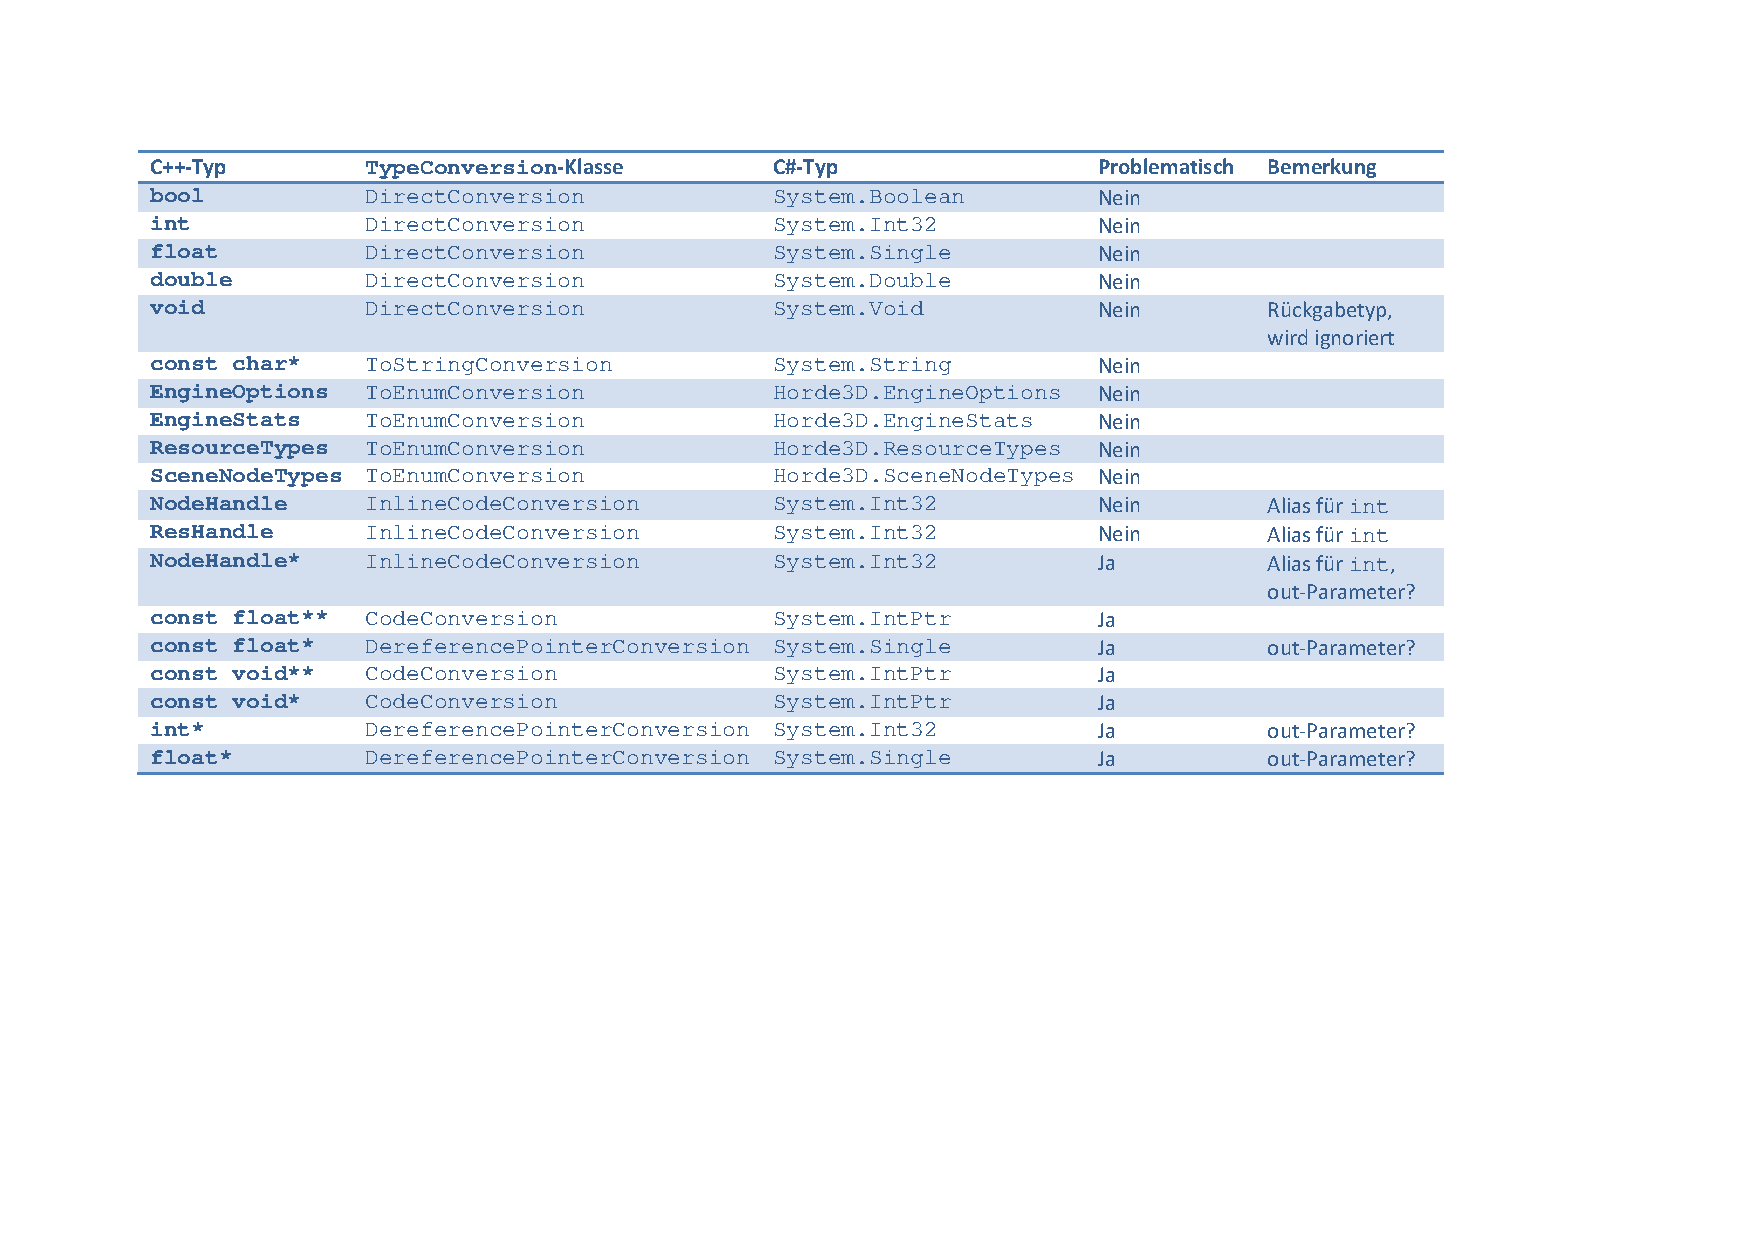
\includegraphics[trim = 20mm 75mm 55mm 20mm, clip, scale= 0.7]{images/CodeGen_Rules.pdf}
\caption{Konvertierungsregeln des Code Generators}\label{fig:cgRules}
\end{figure}	

F�r das Parsen der Funktionen in der \Horde-\emph{Header}-Datei wurden \emph{Regular Expressions} verwendet, wodurch der Parsing-Code kompakt gehalten werden konnte. Auch f�r die Generierung des \Csharp-Codes wurde auf bereits vorhandene .NET-Funktionalit�ten zur�ckgegriffen; .NET enth�lt einen Code Generator f�r \Csharp, Visual Basic .NET und \C++/CLI. Der \C++-Code musste jedoch von Hand durch Konstruktion eines Strings generiert werden, da der .NET Code Generator keinen nativen \C++-Code erzeugen kann.

Die Bestimmung der ben�tigten \texttt{CodeConversionRule}s orientierte sich an den verwendeten Datentypen der \Horde-Funktionen und ist somit nicht allgemein vollst�ndig, sondern nur ausreichend f�r Version 1.0.0 Beta 3 von \Horde. Die Konvertierungsregeln sind in Abbildung~\ref{fig:cgRules} tabellarisch aufgelistet.

%\begin{sidewaystable}[htp]
%	\centering
%		\begin{tabular}{|l|l|l|l|p{3.5cm}|}
%		  \hline
%		  \multicolumn{5}{|c|}{\textbf{Konvertierungsregeln des Code Generators}} \\
%			\hline
%			\C++-Typ & \texttt{TypeConversion}-Klasse & \Csharp-Typ & Problematisch & Bemerkung\\
%			\hline
%			\texttt{bool} & \texttt{DirectConversion} & \texttt{System.Boolean} & nein & \\
%			\texttt{int} & \texttt{DirectConversion} & \texttt{System.Int32} & nein & \\
%			\texttt{float} & \texttt{DirectConversion} & \texttt{System.Single} & nein & \\
%			\texttt{double} & \texttt{DirectConversion} & \texttt{System.Double} & nein & \\
%			\texttt{void} & \texttt{DirectConversion} & \texttt{System.Void} & nein & R�ckgabe-Typ, wird ignoriert\\
%			\texttt{const char*} & \texttt{ToStringConversion} & \texttt{System.String} & nein & \\
%			\texttt{EngineOptions} & \texttt{ToEnumConversion} & \texttt{Horde3D.EngineOptions} & nein & \\
%			\texttt{EngineStats} & \texttt{ToEnumConversion} & \texttt{Horde3D.EngineStats} & nein & \\
%			\texttt{ResourceTypes} & \texttt{ToEnumConversion} & \texttt{Horde3D.ResourceTypes} & nein & \\
%			\texttt{SceneNodeTypes} & \texttt{ToEnumConversion} & \texttt{Horde3D.SceneNodeTypes} & nein & \\
%			\texttt{NodeHandle} & \texttt{InlineCodeConversion} & \texttt{System.Int32} & nein & Alias f�r \texttt{int} \\
%			\texttt{ResHandle} & \texttt{InlineCodeConversion} & \texttt{System.Int32} & nein & Alias f�r \texttt{int}\\
%			\texttt{NodeHandle*} & \texttt{InlineCodeConversion} & \texttt{System.Int32} & ja & Alias f�r \texttt{int}, out-Parameter? \\
%			\texttt{const float**} & \texttt{CodeConversion} & \texttt{System.IntPtr} & ja & \\
%			\texttt{const float*} & \texttt{DereferencePointerConversion} & \texttt{System.Single} & ja & out-Parameter? \\
%			\texttt{const void**} & \texttt{CodeConversion} & \texttt{System.IntPtr} & ja & \\
%			\texttt{const void*} & \texttt{CodeConversion} & \texttt{System.IntPtr} & ja & \\
%			\texttt{int*} & \texttt{DereferencePointerConversion} & \texttt{System.Int32} & ja & out-Parameter? \\
%			\texttt{float*} & \texttt{DereferencePointerConversion} & \texttt{System.Single} & ja & out-Parameter? \\
%			\hline
%			\end{tabular}
%\end{sidewaystable}		

\subsection{Code Generierung nach einem Update der Horde3D-API}
Wenn sich die �ffentliche API einer neuen \Horde-Version ge�ndert hat, muss die Code Generierung erneut ausgef�hrt werden. Um �nderungen, die an den Einstellungen problematischer Funktionen durchgef�hrt wurden, nicht immer wieder machen zu m�ssen, verf�gt der Code Generator �ber einen automatischen Update-Mechanismus. Tabelle~\ref{fig:cgStats} zeigt, wie dieser Mechanismus mit API-Updates zurechtkommt.

%\begin{table}[ht]
%	\centering
%		\begin{tabular}{|p{5.5cm}|l|l|l|l|}
%		  \hline
%		  & \multicolumn{4}{|c|}{\Horde\ Version} \\
%			\hline
%			& 0.0.15 & 1.0.0 Beta 1 & 1.0.0 Beta 2 & 1.0.0 Beta 3 \\
%			\hline
%			\Horde-Funktionen & 67 & 68 & 75 & 78 \\
%			Problematische Funktionen & 9 & 9 & 10 & 10 \\
%			~~~~... bereits als gel�st markiert & - & 9 & 9 & 9 \\
%			~~~~... eigentlich unproblematisch & 3 & 0 & 1 & 0 \\
%			Notwendige �nderungen & 6 & 0 & 0 & 1 \\
%			�nderungen �bernommen & - & 6 & 9 & 9 \\
%			�nderungen verworfen & - & 0 & 0 & 1 \\
%			\hline
%			\end{tabular}
%			\caption{�bersicht �ber die �bernahme von �nderungen an problematischen Funktionen nach einem Update der \Horde-API}\label{tab:updateStats}
%\end{table}		

\begin{figure}[htp]
\centering
%trim=l b r t  	This option will crop the imported image by l from the left, b from the bottom, r from the right, and t  from the top. Where l, b, r and t are lengths. 
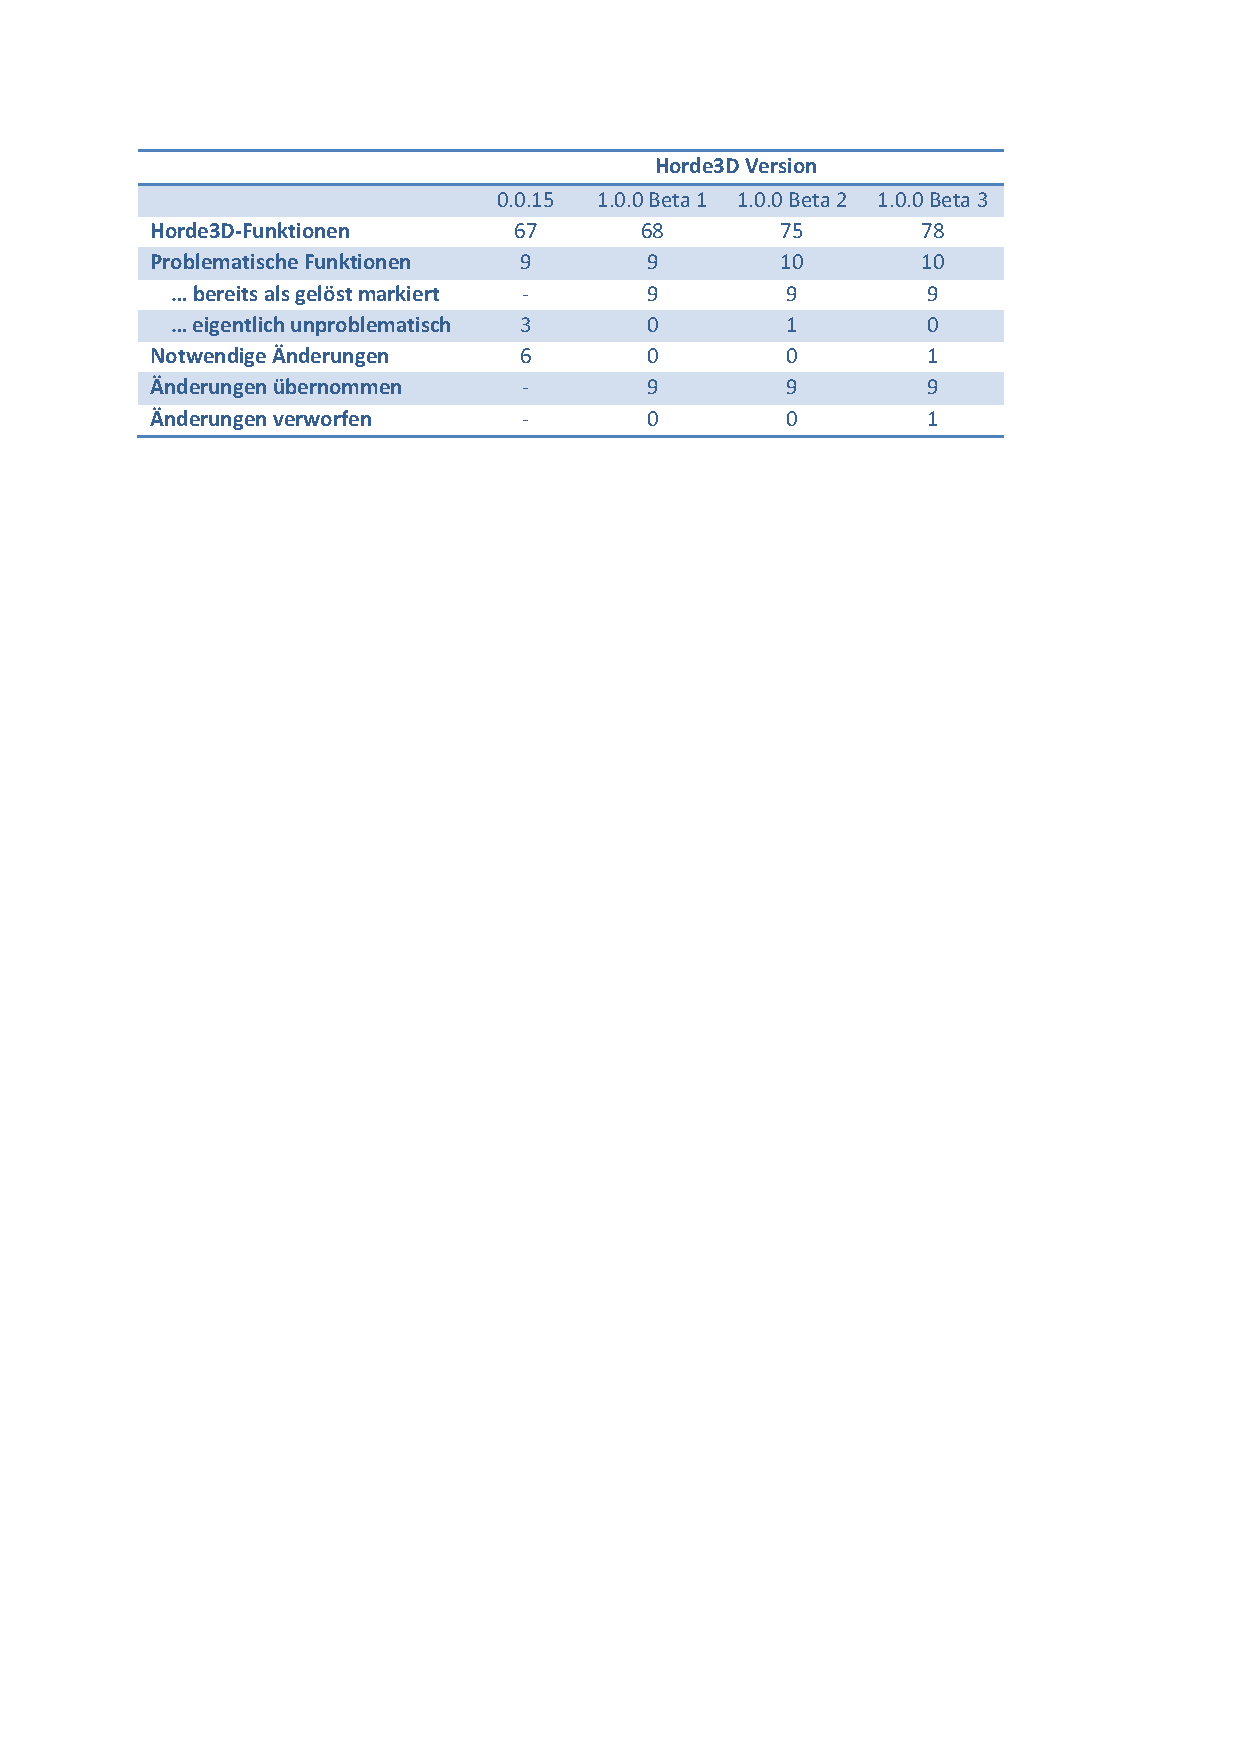
\includegraphics[trim = 20mm 220mm 20mm 20mm, clip, scale = 0.7]{images/CodeGen_Stats.pdf}
\caption{Evaluation des Update-Mechanismus des Code Generators}\label{fig:cgStats}
\end{figure}	

Ausgehend von Version 0.0.15 wurden die API-Updates auf die Betas 1, 2 und 3 von \Horde\ 1.0.0 untersucht. Version 0.0.15 hatte 67 �ffentliche Funktionen, von denen neun als problematisch markiert wurden. Von diesen neun waren wiederum drei eigentlich unproblematisch. Die Annahme, bei Zeiger-Parametern handle es sich eigentlich um \emph{out}-Parameter, war f�r diese drei Funktionen korrekt. Die verbleibenden sechs problematischen Funktionen mussten allerdings wirklich von Hand modifiziert werden. In zwei F�llen konnten \texttt{void}-Zeiger sogar nur als \texttt{System.IntPtr} weitergereicht werden. Ansonsten war es m�glich, \texttt{float}-Zeiger, die Matrizen repr�sentierten, als \texttt{float}-\emph{Arrays} der L�nge 16 weiterzugeben.

Beim Update auf Version 1.0.0 Beta 1 kam eine neue, unproblematische Funktion hinzu. Die manuellen �nderungen konnten alle erfolgreich �bernommen werden, sodass nichts weiter zu tun war und der Code sofort neu generiert werden konnte. Mit Beta 2 kamen weitere Funktionen hinzu, von denen eine als problematisch erkannt wurde. Allerdings war auch hier die \emph{out}-Parameter-Annahme korrekt. Alle manuellen �nderungen von Version 0.0.15 wurden auch bei diesem Update korrekt �bernommen. Beta 3 f�hrte weitere neue Funktionen ein. Beim Update wurde allerdings eine manuelle �nderung verworfen, da die Funktion umbenannt wurde. Umbenannte Funktionen erkennt der Update-Mechanismus nicht. Die �nderung musste also manuell aus den vorherigen Einstellungen kopiert werden; ansonsten waren aber auch in diesem Update-Schritt keine weiteren Anpassungen n�tig.
\section{Client-Server-Kommunikation}
Bei der Implementierung der Client-Server-Kommunikation mit der Windows Communication Foundation konnte das \texttt{IDebuggerService}- und das \texttt{IDebuggerServiceCallback}-Interface aus dem Design unver�ndert �bernommen werden. Aus technischen Gr�nden musste allerdings noch die Service-Operation \texttt{RegisterClient} hinzugef�gt werden. Der Client ruft diese Funktion sofort nach dem Zustandekommen der Verbindung auf, um seinen \emph{Callback Channel} beim Server zu registrieren. Dann erst kann der Server \emph{Callbacks} an den Client schicken.

Es mussten besondere Ma�nahmen getroffen werden, um \emph{Deadlocks} und \emph{Race Conditions} zu vermeiden. Die \Horde-Anwendung kann mehrere Threads verwenden; der Server hat keine M�glichkeit dies herauszufinden und sollte davon auch nicht abh�ngen, da die \Horde-API sowieso nicht \emph{thread-safe} ist. Die Implementierung geht deshalb davon aus, dass alle \Horde-Funktionen vom gleichen Thread aus aufgerufen werden. WCF f�hrt aber jede Anfrage des Clients in einem gerade zur Verf�gung stehenden Thread des \emph{Thread Pools} aus. Da die Service-Operationen zumindest teilweise auf \Horde-Funktionen zugreifen, k�nnte es somit zu \emph{Race Conditions} kommen oder auf inkonsistenten Zust�nden gearbeitet werden. Es musste daher sichergestellt werden, dass jeder Server-Aufruf im gleichen Thread wie \Horde\ l�uft. 

Das .NET Framework bietet die \texttt{SynchronizationContext}-Klasse f�r Threadwechsel an. Der \texttt{Post}-Methode dieser Klasse kann ein \emph{Delegate} �bergeben werden, der in einem ganz bestimmten Thread ausgef�hrt wird. Leider stellt die Standard-Implementierung der Klasse nur die Funktionen bereit, das Wechseln des Threads ist nicht implementiert\footnote{Der Grund daf�r ist, dass es verschiedene M�glichkeiten f�r die Implementierung des Threadwechsels gibt. .NET bietet zwei Implementierungen f�r WinForms und WPF an, die allerdings auch nur von WinForms- und WPF-Anwendungen verwendet werden k�nnen. \Horde-Anwendung k�nnen aber auch die native Win32-API zum Erzeugen des Anwendungsfensters benutzen.}. Es wurde daher der \texttt{Horde3DSynchronizationContext} entwickelt, der von \texttt{SynchronizationContext} erbt. Wird die \texttt{Post}-Methode der Klasse aufgerufen, wird die �bergebene Funktion in einer \texttt{Queue} \emph{thread-safe} protokolliert, aber noch nicht ausgef�hrt. 

Bei jedem Aufruf einer \Horde-Funktion l�st \texttt{Horde3DCall} das \texttt{BeforeFunctionCalled}-Ereignis aus. Der \texttt{Horde3DDebugger} registriert einen \emph{Event Handler}, der beim Ausl�sen dieses Ereignisses die \texttt{Execute}-Methode des \texttt{Horde3DSynchronizationContext}s aufruft. Da die Horde-Funktion und somit auch das Ereignis im \Horde-Thread laufen, werden alle Methoden, die derzeit in der \texttt{Queue} des Synchronisationskontexts liegen, der Reihe nach im \Horde-Thread ausgef�hrt.

Dieses Prinzip stellt sicher, dass alle Aufrufe der WCF-Serverfunktionen im \Horde-Thread laufen. Da WCF sehr flexibel und konfigurierbar entwickelt wurde, kann WCF automatisch eine Instanz des \texttt{Horde3DSynchronizationContext}s zum Wechseln des Threads verwenden. Dazu musste das \texttt{Horde3DThreadAffinityAttribute}-Attribut definiert werden, welches das \texttt{IContractBehavior}-Interface von WCF implementiert. Mit diesem Attribut kann der Synchronisationskontext von WCF programmatisch gesetzt werden \cite{wcf}.

Das Design sah auch vor, dass \emph{Callback}-Aufrufe garantiert an den Client geschickt werden, auch, wenn dieser noch gar nicht verbunden ist. Die \texttt{DebuggerService}-Klasse wurde daher um statische Funktionen f�r jede \emph{Callback}-Operation erweitert, die den \emph{Callback}-Aufruf abfangen und in einen anderen Thread verlagern. Dieser Thread versucht solange den \emph{Callback} auszuf�hren, bis eine Verbindung aufgebaut wurde und der \emph{Callback} erfolgreich durchgef�hrt werden konnte.

Client-seitig werden Serveroperationen immer aus einem \emph{Backgroundthread} aufgerufen, damit die GUI nicht blockiert wird und weiterhin auf Benutzereingaben reagieren kann. Die \texttt{DebuggerServiceProxy}-Klasse k�mmert sich intern um die Verbindung zum Server und die Thread-Verwaltung. Falls der Client noch nicht zum Server verbunden ist, wird vor dem Aufruf der Operation eine Verbindung aufgebaut.

Ein Problem ergab sich durch die Assoziationen zwischen den Ressourcen und insbesondere der \emph{Scene Nodes} untereinander. WCF serialisiert immer den kompletten Objektgraph. Schickt man also beispielsweise einen \emph{Scene Node} an den Client, wird auch dessen Vaterknoten mitgeschickt. Aber auch der Vater des Vaters wird mit �bertragen. Das endet erst beim Erreichen der Wurzel. Um dieses Problem zu vermeiden, werden die Assoziationen �ber die \texttt{NodeHandle}s beziehungsweise \texttt{ResHandle}s identifiziert. Der Client muss dann �ber diese IDs das eigentliche Objekt beim \texttt{SceneGraph}- oder \texttt{ResourceGraph}-Modell erfragen. Die Zuordnung von den IDs zu den Objekten erfolgt �ber eine Hashtabelle, hat also nur die Komplexit�t $O(1)$. Um den Zugriff syntaktisch m�glichst einfach zu halten, ist in der \texttt{Graph}-Klasse ein Indexoperator definiert. Das folgende Beispiel zeigt die Implementierung des \emph{Properties} \texttt{SceneNode.Parent}, das �ber die \texttt{SceneGraph}-Instanz und den \texttt{NodeHandle} des Vaters die Vater-Instanz zur�ckliefert:

\lstset{language=Java} 
\begin{lstlisting}
public class SceneNode
{
	internal int ParentHandle { get; }
	
	public SceneGraph SceneGraph { get; set; }
	
	public SceneNode Parent
	{
		get { return SceneGraph[ParentHandle]; }
	}
	
	// ...
}
\end{lstlisting}

Der Zugriff auf die Vater-Instanz �ber das \texttt{ParentHandle}-\emph{Property} wird komplett gekapselt. F�r den Benutzer der Klasse macht es keinen Unterschied, ob die Vater-Instanz direkt �bertragen wird, oder aus dem \texttt{SceneGraph}-Objekt stammt.
\section{Anhalten der Anwendung}\label{suspendApp}
Das \DevEnv\ verwendet drei verschiedene Implementierungen des \texttt{ISuspendApplicationStrategy}-Interfaces zum Anhalten der Anwendung. Eine Strategie t�uscht dem Prozess vor, dass keine Zeit mehr vergeht. Eine andere leitet alle Tastatur- und Mauseingaben des Benutzers an eine andere Funktion um. Die dritte Klasse zum Fangen und Freilassen des Mauszeigers kam erst nach der zweiten Iteration der Design-Phase hinzu. Dank der Verwendung des \emph{Strategy Patterns} musste jedoch nur eine Zeile Code im Konstruktor der \texttt{SuspendApplicationStrategy}-Klasse hinzugef�gt werden, um die dritte Strategie einzubinden.

Die urspr�ngliche Idee war, den Prozess der Anwendung wirklich anzuhalten. Dazu gibt es die Funktionen \texttt{SuspendThread} und \texttt{ResumeThread} der Win32-API. Mit Hilfe dieser Funktionen kann ein Thread pausiert und wieder fortgesetzt werden. Ruft man diese Funktionen f�r alle Threads eines Prozesses auf, so wird der komplette Prozess eingefroren und wieder fortgesetzt. Dieses Verfahren ist jedoch nicht problemlos anwendbar, da Teile des Prozesses noch weiterlaufen sollten; so sollte WCF in der Lage sein, Anfragen vom Client zu bearbeiten und \emph{Callbacks} auszul�sen. Um das zu gew�hrleisten, darf der Thread, in dem WCF l�uft, nicht angehalten werden. Die Win32-Funktionen arbeiten aber auf nativen Threads, w�hrend WCF in einem \emph{managed} Thread l�uft. Es kann aber passieren, dass die CLR mehrere \emph{managed} Threads im gleichen nativen Thread laufen l�sst. Noch problematischer wird es, wenn die \Horde-Anwendung ebenfalls in .NET geschrieben wurde oder mehrere \emph{AppDomains}\footnote{Eine .NET-\emph{AppDomain} kann man sich als einen .NET-Prozess vorstellen. Es kann in einem nativen Prozess mehrere \emph{AppDomains} geben. Das Betriebssystem kennt das Konzept der \emph{AppDomains} nicht.} im Prozess laufen. Es ist also schwierig genau festzustellen, welche Threads angehalten werden d�rfen. Des Weiteren kommt noch hinzu, dass es verschiedene Versionen der \texttt{Suspend-/ResumeThread}-Funktionen f�r native 32 Bit Prozesse, 32 Bit Prozesse unter einem 64 Bit Betriebssystem und 64 Bit Prozesse gibt.

Derzeit ist f�r das richtige Anhalten des Prozesses keine \texttt{ISuspendApplicationStrategy}-Implementierung vorhanden. In vielen F�llen sind die drei im folgenden vorgestellten Strategien ausreichend. Es gibt aber auch F�lle, in denen ein richtiges Anhalten des Prozesses notwendig w�re. Im folgenden Abschnitt wird auf diese Problematik n�her eingegangen.

\subsection{Anhalten der Zeit}\label{stoptime}
Um den Prozess nicht wirklich anhalten zu m�ssen, wurde eine Idee aus NVIDIAs PerfHUD �bernommen: Das Anhalten der Zeit. Im Benutzerhandbuch gibt es einen Hinweis darauf, wie NVIDIA dieses Problem l�st: 

\begin{quote}"`PerfHUD �freezes� your application by returning the same value every time your application asks for the current time."' \cite[S. 11]{perfhud}\end{quote}

Das ist auch die Vorgehensweise des \DevEnvs. Die meisten Anwendungen verwenden die hochaufl�sende \emph{Timer}-Funktion \texttt{QueryPerformanceCounter}, um die vergangene Zeit zu messen. Jeder Aufruf dieser Funktion wird an eine Funktion des Servers umgeleitet. Dort wird der wirkliche \emph{Timer} aufgerufen und der R�ckgabewert aufgezeichnet. Ist die Anwendung angehalten, wird immer der Zeitwert zum Zeitpunkt des Anhaltens der Anwendung zur�ckgeliefert; die Anwendung meint, es sei seit dem letzten Frame keine Zeit vergangen. Dadurch ist die Zeit angehalten und die Anwendung pausiert. Wird die Anwendung wieder fortgesetzt, so wird wieder der richtige Zeitwert geliefert, abz�glich der Zeitdauer, w�hrend der die Anwendung pausiert war.

\begin{figure}[ht]
\centering
%trim=l b r t  	This option will crop the imported image by l from the left, b from the bottom, r from the right, and t  from the top. Where l, b, r and t are lengths. 
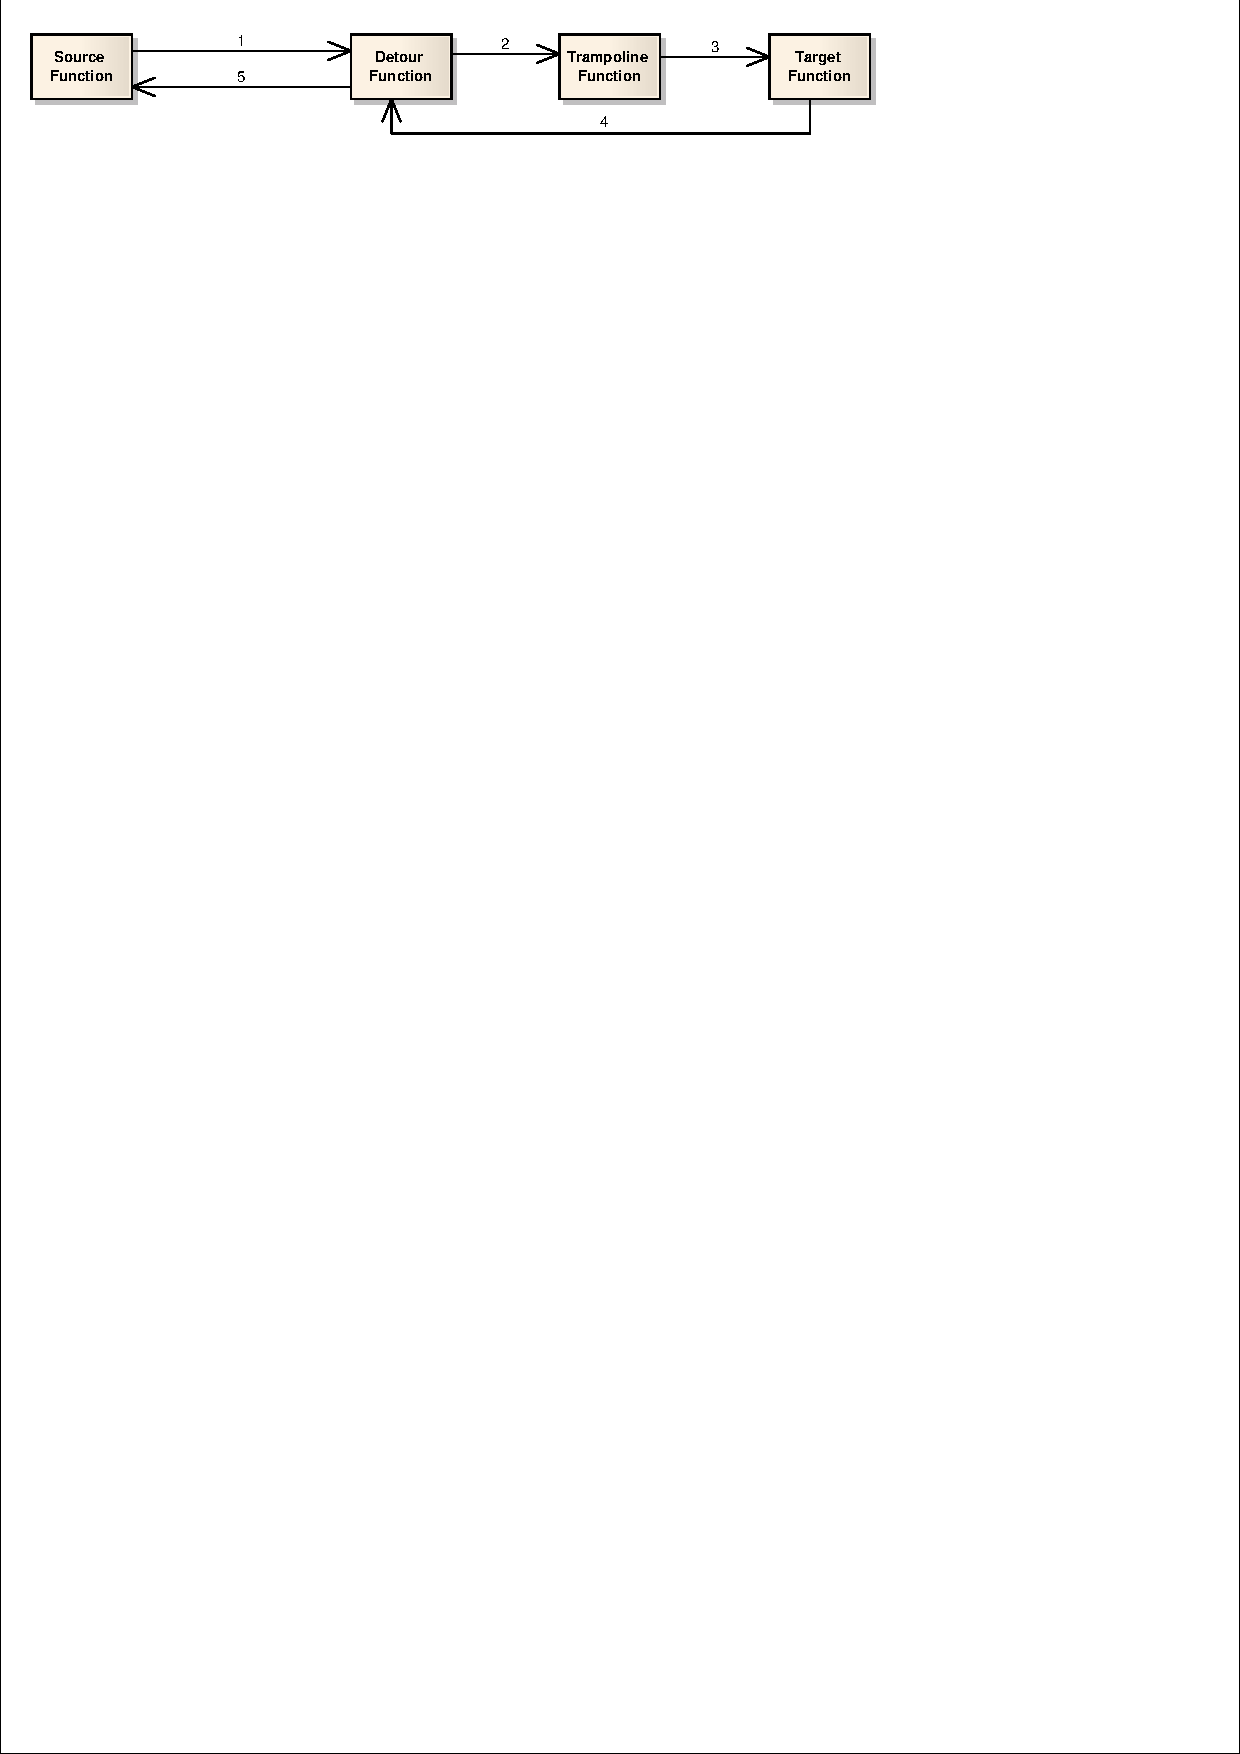
\includegraphics[trim = 5mm 270mm 60mm 5mm, clip, scale=0.7]{images/Detours.pdf}
\caption{Kontrollfluss bei einem abgefangenen Funktionsaufruf}\label{fig:detours}
\end{figure}

Technisch wird das Umleiten des Funktionsaufrufs durch Microsofts Detours Express Bibliothek gel�st. Die Bibliothek kann in einer Anwendung verwendet werden, um einen Aufruf einer beliebigen, nativen Funktionen (\emph{Target Function}) abzufangen und auf eine beliebige selbst definierte Funktionen (\emph{Detour Function}) umzuleiten. Zur Laufzeit schreibt Detours das Abbild des in den Prozess geladenen Bin�rcodes der \emph{Target Function} um. Abbildung~\ref{fig:detours} zeigt den Kontrollfluss beim abgefangenen Aufruf der \emph{Target Function}. Die ersten Instruktionen der \emph{Target Function} werden durch einen Sprung zur \emph{Detour Function} ersetzt. Es wird also als erstes die \emph{Detour Function} ausgef�hrt. Dort kann beliebiger Code abgearbeitet werden. Detours erzeugt au�erdem eine \emph{Trampoline Function}, welche die ersetzen Instruktionen der \emph{Target Function} enth�lt und anschlie�end zur \emph{Target Function} zur�ckspringt. Die \emph{Detour Function} kann die \emph{Trampoline Function} aufrufen, um die \emph{Target Function} auszuf�hren. Verl�sst der Kontrollfluss die \emph{Target Function}, ist wieder die \emph{Detour Function} aktiv und kann weiterhin beliebigen Code ausf�hren. Schlie�lich kehrt der Kontrollfluss zur aufrufenden Funktion (\emph{Source Function}) zur�ck.

Das Anhalten der Zeit hat einige wichtige Konsequenzen: Zum einen funktioniert die Vorgehensweise gar nicht, wenn die Anwendung nicht \texttt{QueryPerformanceCounter} zum Messen der Zeit verwendet. Da es aber keine anderen hochaufl�senden Zeitmesser f�r Windows gibt, wird dies nicht oft der Fall sein. Zum anderen kommt es zu Problemen, wenn die Anwendung nicht so schnell arbeitet wie sie kann, sondern auf eine gewisse Zahl an Updates pro Sekunde festgelegt ist. Falls die Anwendung beispielsweise maximal 60 mal pro Sekunde ein Update ausf�hrt, aber scheinbar seit dem letzten Frame keine Zeit vergangen ist, wird sie einfach gar nichts mehr tun; sie sollte aber wenigstens noch \texttt{Horde3D::render} aufrufen. Gegebenenfalls muss zur Verwendung des \DevEnvs\ die Frameraten-Limitierung abgeschaltet werden. Da beim Starten der Anwendung Kommandozeilenparameter �bergeben werden k�nnen, kann die Abschaltung der Limitierung prinzipiell auch ohne eine �nderung der Anwendung erfolgen, falls die Anwendung per Kommandozeile entsprechend konfigurierbar ist.

Das Vorgehen funktioniert auch nicht, wenn f�r zeitabh�ngige Berechnungen nicht die vergangene Zeit ${\Delta}t$ sondern die aktuellen \emph{Frames Per Second} (FPS) verwendet werden. Da FPS $= 1 / {\Delta}t$ wird die FPS-Berechnung f�r ${\Delta}t = 0$ entweder nicht ausgef�hrt, oder sie liefert keinen vern�nftigen Wert zur�ck.

Die Methode hat auch keinen Erfolg, wenn die Anwendung oder Teile der Anwendung zeitunabh�ngig arbeiten. Denkbar w�re zum Beispiel eine Client-Server-Anwendung, in der der Server kontinuierlich neue Positionen der Objekte berechnet und an den Client schickt. Der Client empf�ngt die Nachrichten des Servers, baut die Szene entsprechend um und zeichnet sie neu. F�r den Benutzer scheint die Anwendung weiterhin zu laufen, obwohl der Client eigentlich angehalten ist und f�r ihn keine Zeit mehr vergeht.

All diese Probleme w�rden nicht auftauchen, wenn der Prozess der Anwendung wirklich angehalten werden w�rde, wie oben beschrieben. Es wurde dennoch aus zwei Gr�nden nur die Zeit-Methode umgesetzt: Erstens ist wie beschrieben beim Anhalten des Prozesses nicht klar, welche Threads angehalten werden d�rfen, wohingegen die Implementierung der Zeit-Methode einfach ist. Zweitens wird die Zeit-Methode in jedem Fall ben�tigt. H�lt man die Threads der Anwendung an, so laufen diese zwar nicht weiter, die Zeit aber schon. Setzt man nun die Threads fort, so k�nnen seit dem letzten Frame mehrere Sekunden oder Minuten vergangen sein. Die Physik- und Animationssysteme rechnen dann mit einem viel zu gro�en ${\Delta}t$ von mehreren Sekunden oder Minuten und k�nnen eventuell keinen stabilen Zustand mehr erreichen.

\subsection{Ersetzen des Window Procedures}
Die Win32-API verwendet Nachrichten, um mit einem Anwendungsprozess zu kommunizieren. Mit den Nachrichten kann die Anwendung �ber alle wichtigen Ereignisse informiert werden: Mausklicks, Tastatureingaben, Mausbewegungen, Schlie�en der Anwendung, Verschieben des Anwendungsfensters, Ablaufen eines \emph{Timers}, und so weiter. Alle Nachrichten an einen Prozess beziehungsweise an ein Fenster werden an eine ausgewiesene Funktion, das \emph{Window Procedure} (\emph{WndProc}), geschickt. Dort wird als Reaktion auf spezielle Nachrichten anwendungsspezifischer Code ausgef�hrt.

Das \DevEnv\ muss auf zwei Arten mit dem \emph{Window Procedure} der Anwendung interagieren: Einerseits muss es Nachrichten abfangen, die f�r den Server eine Bedeutung haben. Dr�ckt der Benutzer beispielsweise die Taste F7, so soll der Server die Anwendung anhalten. Auf der anderen Seite darf das \emph{Window Procedure} der Anwendung keine Benutzereingaben mehr erhalten, wenn die Anwendung angehalten ist. Es soll aber dennoch m�glich sein, das Anwendungsfenster zu verschieben oder zu schlie�en. 

Bei der Initialisierung des Servers wird mit der Win32-Funktion \texttt{SetWindowsHookEx} ein prozessweiter \emph{Hook} aktiviert, der alle Nachrichten an das \emph{WndProc} der Anwendung abf�ngt. Innerhalb des \emph{Hooks} wird �berpr�ft, ob f�r den Server eine relevante Nachricht -- also zum Beispiel \texttt{KeyDown} f�r die Taste F7 -- geschickt wurde. In diesem Fall reagiert der Server entsprechend. Anschlie�end wird die Nachricht an das \emph{WndProc} weitergeleitet.

Mit der Funktion \texttt{SetWindowLongPtr} kann der \emph{WndProc}-Zeiger eines Fensters auf eine beliebige benutzerdefinierte Funktion gesetzt werden. Der Server ersetzt das \emph{Window Procedure} des Anwendungsfensters, wenn die Anwendung angehalten wird. Das \emph{WndProc} des Servers ignoriert alle eingehenden Nachrichten �ber Maus- und Tastatureingaben und behandelt nur Fenster-Nachrichten wie Verschieben oder Schlie�en. Beim Fortsetzen der Anwendung wird der Zeiger wieder auf das urspr�ngliche \emph{WndProc} gesetzt.

\subsection{Freigabe des Mauszeigers}
Viele Anwendungen beschr�nken den Mauszeiger auf ihre Fenstergr��e und verstecken ihn. Beim Testen des \DevEnvs\ mit den Beispielapplikationen des \Horde-SDKs zeigten sich verschiedene Probleme mit dieser exklusiven Benutzung der Maus. Der Server f�ngt daher -- wiederum mit der Detours Express Bibliothek von Microsoft -- alle Aufrufe der Win32-Funktionen \texttt{ShowCursor}, \texttt{ClipCursor} und \texttt{SetCursorPos} ab. Aufrufe dieser Funktionen werden protokolliert und anschlie�end die urspr�nglichen Funktionen aufgerufen. Dadurch kann der Mauszeiger beim Anhalten der Anwendung freigegeben werden und beim Fortsetzen der Anwendung der von der Anwendung gew�nschte Zustand wiederhergestellt werden.
\section{Aufbau der Visual Studio Solution}\label{aufbau}
Die Visual Studio Projektmappe f�r das \DevEnv\ besteht aus mehreren Projekten, die in mehreren Kategorien gruppiert sind. Abbildung~\ref{fig:solution} zeigt einen Screenshot des \emph{Solution Explorers} von Visual Studio und gibt einen �berblick �ber die verschiedenen Projekte.

Die Verzeichnis-Struktur des Projekts im Dateisystem entspricht nicht dem Visual Studio-Standard. Unterhalb des Hauptverzeichnisses gibt es drei weitere Verzeichnisse: bin, in dem alle kompilierten DLLs, die \emph{Executable} des Clients und das Knight-Sample liegen; Dependencies, in dem alle ben�tigten Bibliotheken liegen; und src, in dem der komplette Source Code liegt.

\begin{figure}[ht]
\centering
%trim=l b r t  	This option will crop the imported image by l from the left, b from the bottom, r from the right, and t  from the top. Where l, b, r and t are lengths. 
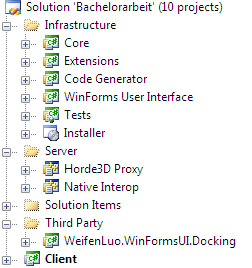
\includegraphics[scale=0.6]{images/Solution.png}
\caption{Aufbau der Visual Studio 2008 \emph{Solution}}\label{fig:solution}
\end{figure}

\subsubsection{Infrastructure}
In der Infrastruktur-Kategorie befinden sich die Projekte, die vom Client und vom Server gemeinsam benutzt werden, sowie der Code Generator und der \emph{Installer}. Alle Projekte dieser Kategorie sind in \Csharp\ geschrieben.

\begin{itemize}
	\item \textbf{Core} (DLL): Diese DLL enth�lt die Kern-Klassen des Systems. Dort befinden sich die Klassen und Interface-Definitionen f�r die Client-Server-Kommunikation, die \Horde-Klassen, die Klassen f�r das Profiling und die \Horde-Meldungen sowie \texttt{Horde3DCall} und \texttt{Horde3DDebugger}.
	
	\item \textbf{Extensions} (DLL): Dieses Projekt stellt einige n�tzliche Erweiterungen f�r das .NET Framework bereit, die vom \DevEnv\ an vielen Stellen verwendet werden.
	
	\item \textbf{Code Generator} (\emph{Executable}): Der Code Generator ist eine eigenst�ndige Anwendung zur Generierung der \Horde-\emph{Proxy}-Funktionen und -Klassen. Zur Laufzeit des Systems wird dieses Projekt nicht ben�tigt.
	
	\item \textbf{WinForms User Interface} (DLL): Diese \emph{Assembly} enth�lt die Implementierung des GUI-Frameworks unter Verwendung der Windows Forms-Klassen.
	
	\item \textbf{Tests} (DLL): Diese Bibliothek enth�lt \emph{Unit Tests} f�r das System. Derzeit gibt es allerdings nur Tests f�r das Parsen der XML-Dateien von Shader-Ressourcen.
	
	\item \textbf{Installer} (\emph{Executable}): Das Projekt erzeugt eine .msi-Datei f�r den Windows \emph{Installer}. Der \emph{Installer} kann das \DevEnv\ auf einem Computer installieren, aktualisieren und wieder l�schen. Alle Voraussetzungen -- .NET 3.5 SP1 und die Visual C++ \emph{Redistributable} f�r 32 Bit Systeme -- werden automatisch installiert.
\end{itemize}

\subsubsection{Server}
Die Server-Projekte sind .NET-\emph{Assemblies}, die in \C++/CLI geschrieben wurden. In \C++/CLI ist der Zugriff auf native Funktionen sowie die Verwendung von Zeigern einfacher und performanter als unter \Csharp. M�chte man diese \emph{Assemblies} debuggen, so ben�tigt man zun�chst eine \Horde-Anwendung, die vom \DevEnv\ gestartet wurde. Anschlie�end kann man die "`\emph{Attach Debugger}"'-Funktionalit�t von Visual Studio verwenden, um den Prozess der Anwendung zu debuggen. Zu beachten ist, dass die DLLs sowohl \emph{managed} als auch nativen Code enthalten. Der Debugger muss daher unbedingt auf "`\emph{mixed mode}"' gesetzt werden, da er ansonsten nur den nativen oder nur den \emph{managed} Teil des Codes sieht.

\begin{itemize}
	\item \textbf{Horde3D Proxy} (DLL): In dieser DLL befinden sich die \Horde-\emph{Proxy}-Funktionen sowie die globale Instanz der \texttt{Horde3DProxyHandler}-Klasse.
	
	\item \textbf{Native Interop} (DLL): Der Server f�hrt einige Aktionen durch, die sehr stark von der Win32-API abh�ngen und daher in \C++/CLI einfacher implementierbar sind. In dieser DLL befindet sich der komplette Code des \emph{Strategy Patterns} zum Anhalten der Anwendung und auch der Code zum Auslesen und Konvertieren des Inhalts eines \emph{Render Targets}.
\end{itemize}

\subsubsection{Third Party}
Zur Zeit befindet sich blo� das Projekt der Weifen Luo Winforms Docking Bibliothek in dieser Kategorie. Das \DevEnv\ verwendet zwar noch weitere Open Source Bibliotheken, diese wurden aber nicht modifiziert. In der \emph{Docking}-Bibliothek wurden hingegen ein paar kleine �nderungen vorgenommen, um das Aussehen der Shell an das von Visual Studio anzugleichen.

\subsubsection{Client}
Der Client ist das eigentliche ausf�hrbare Projekt des \DevEnvs. Vor der Kompilierung des Projekts werden die DLLs, die beim Starten des Servers in das Anwendungsverzeichnis kopiert werden m�ssen, in das \emph{Resources}-Verzeichnis des Client-Projekts kopiert. Der Compiler kompiliert dann die DLLs in die .exe-Datei als .NET-Ressource hinein. Soll der Server gestartet werden, so k�nnen die ben�tigten DLLs aus den Ressourcen ausgelesen werden. Damit entf�llt das fehleranf�llige Kopieren direkt aus dem Anwendungsverzeichnis der Shell.

Da die Verzeichnis-Struktur der \emph{Solution} nicht der Standardstruktur von Visual Studio entspricht, m�ssen zum Debuggen des Clients zwei Projekt-Einstellungen ge�ndert werden. In den Einstellungen muss im Abschnitt "`\emph{Debug}"' die "`\emph{Start Action}"' auf "`\emph{Start external program}"' gesetzt werden. Au�erdem muss der Pfad zur .exe-Datei im bin-Verzeichnis angegeben werden. Das "`\emph{Working Directory}"' muss ebenfalls auf das bin-Verzeichnis gesetzt werden.
\section{Konklusion}
F�r die Implementierung des \DevEnvs\ wurde eine Mischung aus nativem \C++, \C++/CLI und \Csharp\ verwendet. In vielen Bereichen konnten bereits vorhandene Bibliotheken gewinnbringend verwendet werden; insbesondere wurde die Umsetzung der GUI durch die Verwendung der Weifen Luo Winforms Docking Bibliothek und einiger anderer \emph{Controls} deutlich erleichtert. 

Insgesamt wurden weite Teile des Designs erfolgreich umgesetzt. Es wurde jedoch nur der Code entwickelt, der zum Erf�llen der Anforderungen erforderlich war. Gerade bei den \Horde-Klassen sind das Konzept- und auch das Designmodell jedoch detaillierter, als die Anforderungen eigentlich verlangten. An diesen Stellen wurden nur die erforderlichen Teile umgesetzt; die fehlenden Codeteile k�nnen jederzeit erg�nzt werden.

Beim Auslesen der Ressourcen-Daten fiel ein Problem mit der \Horde-API auf: Es gab keine einfache M�glichkeit, alle \Horde\ derzeit bekannten Ressourcen zu ermitteln. Jedoch wurde auf Nachfrage bei den Entwicklern eine entsprechende Funktion in \Horde\ 1.0.0 Beta 3 eingef�hrt. Die API wurde in dieser Version zus�tzlich um eine Funktion erg�nzt, die den Abschluss eines Frames markiert. Der Profiling-Mechanismus ist auf das Vorhandensein dieser Funktion angewiesen. Somit sind diese beiden Funktionen der Grund, warum das \DevEnv\ nur mit Beta 3 kompatibel ist.

Die Implementierung des GUI-Frameworks ben�tigte gegen�ber dem Designmodell einige zus�tzliche Klassen. Die neuen Klassen waren jedoch nur notwendig, um die \texttt{Shell}-, \texttt{Presenter}- und \texttt{IView}-Klassen durch Verwendung von \emph{Generics} typsicher zu machen. Das erm�glichte ein schnelleres Umsetzen der notwendigen \emph{Presenter} und \emph{Views} des \DevEnvs.

Die Erstellung des Code Generators nahm einige Zeit in Anspruch, da zun�chst die Analyse- und Design-Phasen durchlaufen werden mussten. Es zeigte sich jedoch, dass rund 4800 Zeilen Code automatisch generiert werden konnten und nicht von Hand eingetippt werden mussten. Da der Code Generator auch gut mit Updates der \Horde-API zurecht kommt, hat sich auch die detaillierte Analyse der Anforderungen und der m�glichen Probleme bei der Code Generierung gelohnt. Durch die Verwendung des GUI-Frameworks bei der Implementierung der Benutzeroberfl�che des Code Generators hielt sich der Implementierungsaufwand in Grenzen. Zudem konnten fr�h erste Erfahrungen im Umgang mit dem GUI-Framework gesammelt werden und einige Unsch�nheiten bei der Typsicherheit, der Sichtbarkeit von eigentlich internen \emph{Properties} sowie dem thread-sicheren Zugriff auf die \emph{View} eines \emph{Presenters} behoben werden.







%\chapter{Entwicklung eines Hitzeschimmer-Effekts f�r SheepMeUp}

%\section{Implementierung der Special Effects in SheepMeUp}

%\section{Grundlagen eines Hitzeschimmer-Effekts}

%\section{Umsetzung des Effekts}

\chapter{Evaluation und Ausblick}

W�hrend der Entwicklung des \DevEnvs\ wurden bereits verschiedene St�rken, eventuelle Schw�chen und Erweiterungsm�glichkeiten offensichtlich. Es wurde daher nach Abschluss der Entwicklungsarbeiten �berpr�ft, ob das Tool die Anforderungen erf�llt. Dazu wurde zun�chst am Beispiel von \SheepMeUp\ getestet, wie gut das Tool mit bereits bestehenden Anwendungen zusammenarbeitet. Anschlie�end wurde f�r einen Prototyp eines Spiels ein Special Effect f�r den Schild eines Raumschiffes umgesetzt. Es wurden au�erdem einige Entwickler aus der Horde-Community gebeten, das Tool zu testen und an einer Meinungsumfrage teilzunehmen, deren Ergebnisse im folgenden ebenfalls vorgestellt werden. Zuletzt wird noch auf einige Ideen f�r Erweiterungsm�glichkeiten und Verbesserungen eingegangen, die w�hrend der Entwicklung des Tools, der Umsetzung des Schild-Effekts oder beim Testen durch die Community-Mitglieder aufgekommen sind. 

\section{Zusammenarbeit mit SheepMeUp}\label{smuport}
\SheepMeUp\ wurde urspr�nglich f�r die \Horde-Version 1.0.0 Beta 1 entwickelt und musste zun�chst auf Beta 3 portiert werden. Die Portierung erwies sich als schwierig, umfangreich und zeitaufw�ndig, da das komplette Shader-System und gro�e Teile des Material-Systems mit Beta 3 ge�ndert wurden. Es war innerhalb eines ver\-n�n\-ftigen Zeitrahmens daher nicht m�glich, das Spiel voll funktionsf�hig und spielbar auf Beta 3 zu portieren. Die Portierung war jedoch soweit erfolgreich, dass das Spiel wieder lief und nur einige grafische Effekte -- wie Kraftfelder, Fackeln, sowie alle Men�-Elemente -- fehlten. Dies reichte aber bereits aus, um das \DevEnv\ mit \SheepMeUp\ verwenden zu k�nnen.

Es traten jedoch einige Kompatibilit�tsprobleme mit \SheepMeUp\ auf. Diese lagen zwar im Spiel selbst begr�ndet, zeigten aber auch, dass die idealisierten Annahmen, die bei der Entwicklung des \DevEnvs\ getroffen wurden, in der Realit�t nicht immer zutreffen. Im folgenden werden die Probleme und ihre L�sung kurz aufgef�hrt:

\begin{itemize}
	\item \SheepMeUp\ verwendete keine Originalversion der Horde3D DLL, sondern eine um die Funktion \texttt{castRayAABB} erweiterte Variante. Da das Spiel diese Funktion jedoch nicht aufruft, konnte einfach die Original-DLL verwendet werden. Andernfalls h�tte mit dem Code Generator eine angepasste Version des DLL-\emph{Replacement}-Codes generiert werden m�ssen.
	
	\item Anstatt die vergangene Zeit seit dem letzten Frame f�r zeitabh�ngige Berechnungen zu verwenden, wurden die aktuellen \textit{Frames Per Second} (FPS) verwendet. Die FPS wurden jedoch �ber einen Zeitraum von einigen Frames gemittelt, spiegelten also nicht exakt die vergangene Zeit wider. Wird die Anwendung mit dem \DevEnv\ pausiert, so ist die vergangene Zeit seit dem letzten Frame $\Delta t = 0$. In diesem Fall wurden jedoch die FPS nicht aktualisiert. Das f�hrte dazu, dass Schafe, Schockwelleneffekte, die Manaregeneration, zuf�llig abgespielte Sounds und Partikeleffekte nicht mit $\Delta t = 0$ sondern mit einem falschen FPS-Wert berechnet wurden. Die Physik-Engine wurde jedoch angehalten; so bewegten sich die Schafe beispielsweise weiter, aber flogen durch Hy�nen und W�nde hindurch. Aufgrund der Ungenauigkeit der FPS-Berechnung sollte immer der wirkliche $\Delta t$-Wert f�r zeitabh�ngige Berechnungen verwendet werden. Da alle Klassen des Spiels auf diesen Wert zugreifen k�nnen, war eine Anpassung von \SheepMeUp\ innerhalb k�rzester Zeit umgesetzt. 
	
	\item Die Bewegung der K�fer auf dem Boden des Levels waren �berhaupt nicht von der Zeit abh�ngig; die K�fer wurden also je nach H�he der FPS schneller oder langsamer. Da die Bewegung zeitunabh�ngig war, konnte das \DevEnv\ die K�fer auch nicht anhalten. Das war ein Bug des Spiels, der ebenfalls schnell behoben werden konnte. 
	
	\item Ein weiterer Fehler steckte in der Sound-Komponente der verwendeten Game Engine der Universit�t Augsburg. Dort wurde die Geschwindigkeit des \emph{Listeners} unter anderem aus der Differenz zwischen aktueller Zeit und der Zeit des letzten Frames berechnet. Ist die Anwendung angehalten, ist diese Differenz $\Delta t = 0$. Innerhalb der Sound-Bibliothek wurde dann zur Berechnung der Geschwindigkeit des \emph{Listeners} durch $\Delta t = 0$ dividiert, was bei manchen Soundkarten-Treibern zu Abst�rzen f�hrte. Dieser Bug der Game Engine konnte durch eine �berpr�fung auf den Wert $0$ vor dem Funktionsaufruf schnell behoben werden.
\end{itemize}

Nach Behebung dieser Bugs arbeitete das \DevEnv\ problemlos mit \SheepMeUp\ zusammen. Da jedoch aufgrund der Portierung des Spiels auf die aktuelle \Horde-Version die Special Effects nicht mehr funktionierten, konnte \SheepMeUp\  nicht als Grundlage f�r die Implementierung eines neuen Effekts mit Hilfe des \DevEnvs\ dienen.

\section{Umsetzung eines Special Effects f�r Raumschiff-Schilde}\label{space}

F�r einen Prototyp eines Spiels -- ein Raumschiff-Shooter in Top-Down-Ansicht -- wurde ein Effekt f�r das Auftreffen eines Geschosses auf den Schild eines Raumschiffs umgesetzt. Abbildung~\ref{fig:shields} zeigt eine Momentaufnahme des Effekts. Das Raumschiff in der Mitte wurde von rechts von einem Geschoss getroffen. Die beiden blauen Ringe stellen Energiewellen dar, die durch die Absorption des Schusses durch den Schild laufen.

\begin{figure}[ht]
\centering
%trim=l b r t  	This option will crop the imported image by l from the left, b from the bottom, r from the right, and t  from the top. Where l, b, r and t are lengths. 
\includegraphics{images/shields.png}
\caption{Momentaufnahme des Schild-Effekts}\label{fig:shields}
\end{figure}

Es stellte sich heraus, dass das \DevEnv\ in diesem Szenario seine St�rken sehr gut ausspielen kann. Zun�chst wurde der Effekt in das Spiel mit einem Standard-Shader, der alles einfach wei� zeichnete, eingebaut. Anschlie�end wurde das Spiel mit dem \DevEnv\ gestartet und der Effekt implementiert. W�hrend der Umsetzung des Effekts musste das Spiel kein einziges mal neu gestartet oder neu kompiliert werden. 

Der Shader des Effekts besteht im wesentlichen aus der Berechnung von Sinus- und Cosinus-Wellen, die in Abh�ngigkeit von der Treffposition des Geschosses und der seit dem Treffer vergangenen Zeit berechnet werden. Die Wellen werden zus�tzlich in Abh�ngigkeit von der Zeit und von der Entfernung zum Treffpunkt ausgeblendet. Der gr��te Vorteil konnte dabei aus der sofortigen Anzeige der �nderungen gezogen werden. Beispielsweise konnte direkt nach der Anpassung einer Konstante der ge�nderte Shader Code an das Spiel �bergeben und die Auswirkungen beurteilt werden. Da dies im Bruchteil einer Sekunde ohne Neustart des Spiels m�glich ist, konnten sehr schnell gute Ergebnisse erzielt werden. Da das \DevEnv\ auch sofort etwaige Probleme beim Kompilieren des Shaders anzeigte, konnten Fehler im Code schnell gefunden werden.

Problematisch bei der Entwicklung von Shadern ist das Debugging. Es gibt zwar Tools wie glslDevil\footnote{\url{http://www.vis.uni-stuttgart.de/glsldevil}} der Universit�t Stuttgart zum Debuggen von GLSL-Shadern, diese sind aber  noch nicht sehr ausgereift. Es bleibt also nur die M�glichkeit zu klassischem "`\texttt{printf}-Debugging"', angepasst auf Shader: Will man den Wert einer Variable wissen, so muss man die Variable als Ausgabe des Shaders -- also die Farbe des Pixels -- setzen und sich die Szene ansehen. Aus den Farbinformationen lassen sich dann R�ckschl�sse auf den eigentlichen Wert der Variable ziehen. Diese Art des Debuggings wird vom \DevEnv\ schnell und unkompiliziert unterst�tzt und erleichtert es erheblich, fehlerhafte Shader zu debuggen.

W�hrend der Entwicklung des Effekts zeigte sich, dass der Shader eine Textur als Eingabe ben�tigt. Dazu wurde das Material des Effekts angepasst und dort die Textur als Eingabe f�r den Shader festgelegt. Da beim Aktualisieren des ge�nderten Materials im Spiel automatisch auch die neue Textur geladen wurde, war auch hier kein Neustart des Spiels notwendig und die �nderungen konnten sofort beobachtet werden.

Der Effekt sollte schlie�lich noch durch eine Verzerrung des Raumschiff innerhalb des Schildes verbessert werden. F�r eine solche Verzerrung ben�tigt der Shader zus�tzlich die komplett gezeichnete Szene als Eingabe. Mit dem \DevEnv\ wurde die Pipeline-Konfiguration des Spiels ge�ndert und ein \emph{Render Target} mit dem Szenen-Inhalt f�r den Shader bereitgestellt. Dabei war es hilfreich, den Inhalt des \emph{Render Targets} betrachten zu k�nnen, um Fehler in der Pipeline-Konfiguration und den Shadern zu beheben. Nach der Erweiterung des Shader Codes konnte der verbesserte Effekt wieder sofort im Spiel betrachtet werden.

Insgesamt erleichtert das \DevEnv\ die Entwicklung neuer Effekte haupts�chlich durch das sofortige Anzeigen der �nderungen sowie durch das sofortige Anzeigen von Problemen beim Kompilieren von Shadern, Einlesen von Materials, etc. Aber auch das �ndern von Texturen von Materials sowie der gesamten Pipeline-Konfiguration ist deutlich einfacher. Der Shader-Designer erwies sich gerade beim Einstellen der Kontext-Parameter wie Blend-Modi, Tiefentests, etc. als sehr hilfreich, weil man die entsprechenden Werte nicht auswendig wissen musste. Ein Gro�teil der Umsetzung des Shaders wurde im Designer erledigt; die zugrundeliegende XML-Datei wurde nur in wenigen F�llen direkt bearbeitet. Der XML-basierten Konfiguration der Pipeline und des Materials w�re ein �hnlicher Designer ebenfalls �berlegen gewesen.

\section{Meinungsumfrage}

\begin{figure}[htp]
\centering
%trim=l b r t  	This option will crop the imported image by l from the left, b from the bottom, r from the right, and t  from the top. Where l, b, r and t are lengths. 
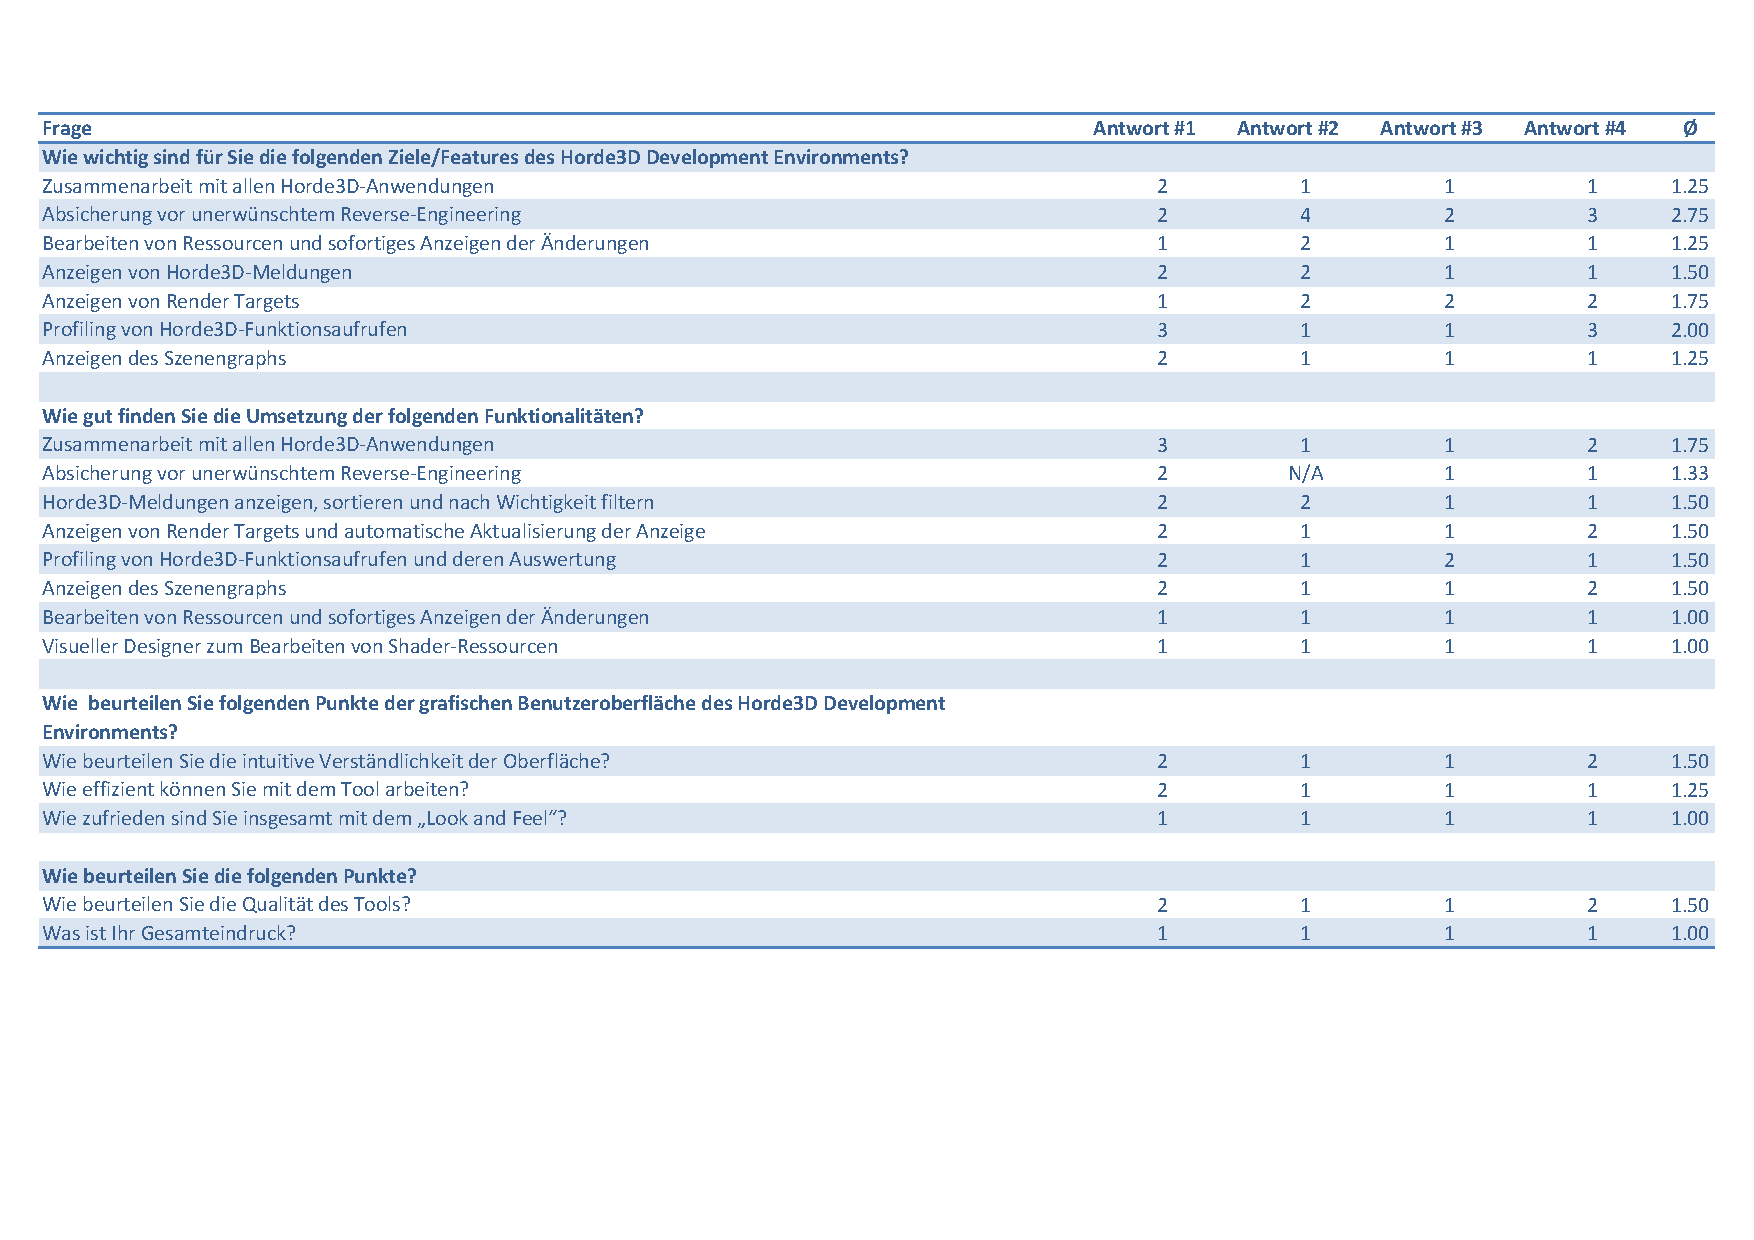
\includegraphics[angle= 90, trim = 1mm 50mm 1mm 10mm, clip, scale=0.7]{images/Fragebogen_Auswertung.pdf}
\caption{Auswertung der Meinungsumfrage}\label{fig:umfrage}
\end{figure}

Es wurden einige Mitglieder der \Horde-Community gebeten, das Tool zu testen und einen Fragebogen auszuf�llen. Zwei Mitglieder des \SheepMeUp-Entwicklungsteams, ein Entwickler von Alfred und einer der Entwickler von \Horde\  nahmen an der Meinungsumfrage teil. Die Fragen und die Bewertungen der Teilnehmer werden in Abbildung~\ref{fig:umfrage} aufgelistet.

Zun�chst wurde gefragt, wie wichtig den Teilnehmern die einzelnen Anforderungen sind, die an das \DevEnv\ gestellt wurden. Dabei f�llt auf, dass der Schutz vor unerw�nschtem \emph{Reverse-Engineering} insgesamt das unwichtigste Feature ist, aber dennoch f�r die Teilnehmer von Bedeutung ist. Erwartungsgem�� wurde die Hauptaufgabe des Tools -- das Bearbeiten von Ressourcen und das sofortiges Anzeigen der �nderungen -- zusammen mit der Kompatibilit�t zu allen \Horde-Anwendungen als am wichtigsten betrachtet.

Die Umsetzung der Ressourcenbearbeitung wurde �bereinstimmend als sehr erfolgreich betrachtet, w�hrend es bei der Kompatibilit�t laut Meinung der Teilnehmer noch Nachbes\-ser\-ungsbedarf gibt. Darauf wird in Abschnitt~\ref{Ausblick} noch eingegangen. 

Insgesamt ist der Gesamteindruck des Tools bei allen Teilnehmern sehr positiv ausgefallen. Dies spiegelt sich nicht nur in der Umsetzung der einzelnen Anforderungen wider, sondern auch an den Bewertungen der Oberfl�che und des \textit{Look and Feels} der Anwendung. Die beiden wichtigsten Fragen\footnote{Ja/Nein-Fragen sowie Freitext-Antworten sind in Abbildung~\ref{fig:umfrage} nicht aufgelistet.}, ob das Tool die Entwicklung von \Horde-Anwendungen erleichtere und ob sich die Teilnehmer vorstellen k�nnten, zuk�nftig das \DevEnv\ zur Entwicklung von \Horde-Anwendungen zu verwenden, wurden einstimmig mit "`ja"' beantwortet.

Im Hinblick auf Kapitel~\ref{abgrenzung} und die teilweise �berlappende Funktionalit�t des \DevEnvs\ und des Horde3D Scene Editors wurden die Teilnehmer gefragt, ob sie ein �hnliches Tool kennen und gegebenenfalls auch bevorzugen w�rden. Die �ber\-ein\-stimm\-ende Meinung war, dass der Szenen-Editor zwar teilweise �hnliche Features biete, aber doch einen grunds�tzlich anderen Fokus habe, und man daher beide Tools problemlos parallel einsetzten k�nne.

Abschlie�end wurden die Teilnehmer nach Verbesserungsvorschl�gen und Ideen f�r Erweiterungen gefragt. Es gab zwei Antworten, die teilweise in Abschnitt~\ref{Ausblick} noch einmal aufgegriffen werden:

\begin{quote}
"`Ein f�r mich interessantes Feature w�re noch Overlays w�hrend der Laufzeit laden zu k�nnen und beliebig �ber das Horde-Fenster zu positioneren und zu strecken. Die Anordnung soll dann als Snapshot abgespeichert werden k�nnen. Dieser "`Designer"' f�r Overlays fehlt mir noch in allen Horde3D Produkten.

Eine weitere Erweiterungsm�glichkeit sehe ich in einem Plugin-System, welches es erlaubt das Horde3D Development Environment um zus�tzliche Editoren und Views zu erweitern.

Dar�ber hinaus w�re es interessant, Texturen prozedural erzeugen zu k�nnen und diese w�hrend Laufzeit einzusetzen."'
\end{quote}

\begin{quote}
"`Ich bin sehr zufrieden mit dem Programm. F�r die Zukunft k�nnte es interessant sein, DLL-Injection-Methoden zu untersuchen um die Kompatibilit�t zu verbessern. Ansonsten k�nnte man den Texture Browser etwas ausbauen (Anzeige von DDS)."'
\end{quote}

\section{Ausblick}\label{Ausblick}

Wie bereits mehrfach angedeutet wurde, gibt es eine Vielzahl an m�glichen Erweiterungen und Verbesserungen f�r das \DevEnv. In diesem Abschnitt werden einige Punkte vorgestellt und kurz erl�utert.

\begin{itemize}
	\item \textbf{Plugin-System.} Ein Plugin-System wurde auch von einem der Umfrageteilnehmer genannt und w�re eine wichtige Erweiterung f�r die Shell, um zuk�nftige neue Features und die Kernfunktionalit�t sauber trennen zu k�nnen. Es gibt bereits einige \Horde-Erweiterungen, wie zum Beispiel f�r Sound-Ausgabe\footnote{\url{http://www.horde3d.org/wiki/index.php5?title=Sound_Extension}}, die mit einem Plugin-System ebenfalls einfach an das Tool angeschlossen werden k�nnten.
	
	\item \textbf{Verbesserung des DLL-\emph{Replacement}-Mechanismus.} Der DLL-\emph{Re\-place\-ment}-Me\-ch\-anis\-mus sollte in zuk�nftigen Versionen verbessert werden. Die Kompatibilit�t mit allen \Horde-Anwendungen ist eines der wichtigsten Ziele des \DevEnvs. Derzeit funktioniert das DLL-\emph{Replacement} nur bei Verwendung der Original-DLL von \Horde. Der Code Generator lie�e sich prinzipiell aber leicht so erweitern, dass der Code f�r die Einstiegspunkte beliebiger \Horde-Extensions ebenfalls generiert wird. Wie ein Teilnehmer an der Meinungsumfrage bereits angedeutet hat, k�nnten andere \emph{Hooking}-Methoden\footnote{siehe zum Beispiel \url{http://www.codeplex.com/easyhook/Thread/View.aspx?ThreadId=35209}} im Allgemeinen eventuell �berlegen sein.
	
	\item \textbf{"`Offline"' Ressourcenverarbeitung.} Das \DevEnv\ un\-ter\-st�tzt derzeit nur die Bearbeitung von Ressourcen, w�hrend oder nachdem eine \Horde-Anwendung gelaufen ist. Es w�re von Vorteil, auch ohne laufende Anwendung -- also quasi "`offline"' -- Funktionen wie den Shader Designer verwenden zu k�nnen.
	
	\item \textbf{Vernetzung der Daten.} Wie man bereits im Konzeptmodell erkennen konnte, sind die einzelnen \Horde-Klassen eng miteinander verbunden. \Horde\ bietet f�r fast alle dieser Beziehungen die M�glichkeit an, diese nachtr�glich auszulesen. Das \DevEnv\ k�nnte diese Informationen nutzen, um beispielsweise alle \emph{Scene Nodes} anzuzeigen, die eine gewissen Ressource verwenden, oder umgekehrt. Auch k�nnten Fehler- und Debug-Meldungen der Engine mit den zugeh�rigen Ressourcen oder \emph{Scene Nodes} verkn�pft werden. Meldungen �ber eine fehlgeschlagene Shader-Kompilierung k�nnten per Doppelklick sofort zur fehlerhaften Zeile f�hren.
	
	\item \textbf{Ausbau und Erg�nzung von Designern.} Wie die Entwicklung des Schild-Effekts zeigte, ist der Shader-Designer eine gro�e Unterst�tzung beim Entwickeln eines Shaders. Die derzeitige Implementierung hat jedoch noch einige Limitierungen, die behoben werden sollten. So k�nnen keine neuen Shader \emph{Sections}, Kontexte, \emph{Sampler} oder \emph{Uniforms} angelegt werden; dies muss in der zugrundeliegenden XML-Datei geschehen. Au�erdem werden Kommentare in der XML-Datei vom Designer gel�scht. �hnlich aufgebaute Designer w�ren ebenfalls f�r Pipelines, Materials und Partikel denkbar. Interessant w�re hier auch, die Ressourcen enger zu verkn�pfen. W�hlt man beispielsweise in einem Material eine Textur f�r einen \emph{Sampler} aus, so k�nnte man dies an Stelle der h�ndischen Eingabe des Pfades der Textur �ber eine \emph{Drop-Down}-Auswahl umsetzen. Die Designer k�nnten auch �berpr�fen, ob die Pfade alle korrekt sind, ohne dass daf�r extra die \Horde-Anwendung gestartet werden muss.
	
	\item \textbf{Einfrieren der Szene.} Das Einfrieren der Szene erm�glicht es, zeitabh�ngige Effekte in einem festen Zustand bearbeiten zu k�nnen. Hier w�re es von Vorteil, durch Verlangsamen oder Beschleunigen der Zeit der \Horde-Anwendung schneller oder pr�ziser zu der Stelle des Effekts zu kommen, die gerade relevant ist. Im eingefrorenen Zustand w�rde au�erdem eine \emph{Free-Look} Kamera die Betrachtung des eingefrorenen Effekts von allen Richtungen m�glich machen. Wie bereits in Kapitel~\ref{stoptime} ausgef�hrt, ist das Anhalten der Zeit problematisch. Hier m�sste nach weiteren L�sungsm�glichkeiten gesucht werden. Eventuell muss das komplette Anhalten der Threads doch implementiert werden, um Client-Ser\-ver-An\-wen\-dungen einfrieren zu k�nnen. Aufgrund der Verwendung des \textit{Strategy Patterns} w�re auch eine Auswahl der verwendeten Algorithmen durch den Benutzer pro \Horde-Anwendung leicht umsetzbar.
	
	\item \textbf{Ausbau der Profiling-Funktionalit�t.} Die Profiling-Funktionalit�t wurde von den Umfrageteilnehmern als unwichtigstes Feature betrachtet, l�sst aber dennoch Raum f�r einige interessante Erweiterungsm�glichkeiten. So werden bei einem Funktionsaufruf bereits der R�ckgabewert und die Werte der Funktionsparameter protokolliert. Die Shell k�nnte diese Daten anzeigen, damit der Benutzer einen besseren �berblick �ber die \Horde-Funktionsaufrufe erh�lt. Au�erdem k�nnten dadurch Funktionsaufrufe mit den Ressourcen oder den \emph{Scene Nodes} verkn�pft werden, die als Parameter �bergeben wurden. Auch w�re es interessant, \Horde-Fehlermeldungen dem Funktionsaufruf zuzuordnen, der den Fehler erzeugt hat.
	
	\item \textbf{Integration oder Anbindung von Third-Party-Anwendungen.} Es gibt \emph{Third-Party}-Anwendungen, deren Integration oder enge Verkn�pfung mit dem \DevEnv\ die Produktitiv�t des Benutzers erh�hen k�nnten. Denkbar w�re beispielsweise eine Anbindung an glslDevil, um Shader debuggen zu k�nnen; eine Integration von SVN, um ge�nderte Ressourcen gleich in das \emph{Repository} einchecken zu k�nnen; oder die Anbindung von Tools wie der Collada Converter von \Horde\ oder FX Composer und RenderMonkey.

\end{itemize}

%# Plugin system
%
% #Auf einfache Erweiterbarkeit ausgelegt
%
%- Anbindung an Shaderdebugger (glsldevil) m�glich? (direkt oder �ber Replay-Funktion)
%
% #Standalone resource editing
%
% -Aufzeichnen des aktuellen Zusstands der Anwendung und dann replay
%
% #Komplette Contentverwaltung (was wird wo benutzt, was wird nie ben�tigt), Colladaconverter integrieren
%
%#FunctionCalls verweisen auf zugeh�rige Resource/SceneNode
%
%#Geschwindigkeit setzen (Zeitmultiplikator)
%
% -Mehr Versionsf�hig (d.h. mehrere Horde3D-Dlls im Debugger speichern und Auswa-hlm�g-lichkeit pro Pro-jekt)
%
%#Kommentare in XML Files gehen durch DShaderesigner verloren
%
% #Shader designer ausbauen
%
% Undo/Redo vern�nftiger machen
%
% #Urspr�ngliche Idee: Verkn�fpung SceneNodes/Resources/Messages
%
% #FunctioNCall params anzeigen
%
% #Unterst�tzung von Extensionss
%
%#Integration mit RenderMOnkey/fx composer
%
%#dll replacement durch was besseres ersetzen?
%
%#weitere strategien um thread anzuhalten x32/x64, SuspendApplicationStragey erweitern und verwendete strategien konfigurierbar machen (z.B. wichtig bei lwar)
%
%#svn integration
%
%#kopieren von resourcenpfadnmane (z.b. textur in material)
%
%-problem: maus caputre + verschieben des fensters
%
%#kamerareplacment: free look, zeit anhalten/verlangsamen
%
%#fehlermeldungen von horde3d nutzen, um fehlerhafte shader zeilen zu markieren
%

\section{Konklusion}

Die Anforderungen an das \DevEnv\ wurden ausgehend von den Erfahrungen bei der Entwicklung von \SheepMeUp\ formuliert und in einem \textit{Unified Process}-�hnlichen Vorgehen systematisch umgesetzt. Die detaillierte Analyse der Anforderungen und der \Horde-Engine f�hrten zu einem umfangreichen, aber flexiblen Design, das schlie�lich schnell und weitestgehend problemlos implementiert werden konnte. Dabei wurde eine Vielzahl an Problemen gel�st und generische Frameworks f�r die GUI-Anbindung und die Code Generierung entwickelt.

Durch die Umsetzung eines Schild-Effekts und einer Umfrage unter mehreren \Horde-Community-Mitgliedern konnte auch best�tigt werden, dass die Anforderungen nicht nur ein Spezialfall der \SheepMeUp-Entwicklung waren, sondern auch f�r andere Anwender und Anwendungen interessant sind. Die Verwendung des \DevEnvs\ f�hrt zu einem teilweise erheblichen Produktivit�tsgewinn bei der Entwicklung von Special Effects f�r \Horde-Anwendungen. Davon profitieren jedoch nicht nur die Entwickler, die Zeit und Geld sparen, sondern vor allem auch deren Kunden und Benutzer, die in k�rzerer Zeit ein qualitativ besseres Produkt erhalten. Es zeigte sich aber auch das Potential, das in zuk�nftigen Versionen des \DevEnvs\ steckt; die Liste der m�glichen Erweiterungen ist umfangreich und viele der Punkte w�rden die Produktivit�t um einen weiteren Faktor erh�hen.

Beim Entwurf und der Konzeption des \DevEnvs\ wurde oft an zuk�nftige Erweiterungen gedacht und bereits einige Vorkehrungen getroffen. Zus�tzlich wurden �nderungen ber�cksichtigt, die an \Horde\ geplant sind oder m�glicherweise eines Tages kommen werden. 

In der n�chsten Version von \Horde\ wird sich das Shader-System ein weiteres mal -- wenn auch nicht so umfangreich wie beim Umstieg auf Beta 3 -- �ndern, um eine HLSL/CG-�hnlichere Syntax zu unterst�tzen. Aufgrund des modularen Designs des Tools wird diese Umstellung aber nur einige wenige lokale �nderungen an der Shell erfordern. �nderungen der \Horde-API k�nnen mit Hilfe des Update-Mechanismus des Code Generators innerhalb von wenigen Sekunden �bernommen werden. 

Die n�chste \Horde-Version wird zus�tzlich einige interessante Erweiterungen zum Abfragen von Ressourcen-Verkn�pfungen und -Daten beinhalten, von denen einige geplante Erweiterungen des \DevEnvs\ profitieren k�nnten. Wenn die immer wieder aufkommende Lizenzdiskussion\footnote{\url{http://www.horde3d.org/forums/viewtopic.php?f=1&t=744&hilit=license}} endg�ltig gekl�rt ist, besteht au�erdem die Hoffnung auf einen neuen Extension-Mechanismus f�r \Horde. Erweiterungen m�ssten dann nicht mehr statisch in die Horde3D DLL gelinkt werden, sondern k�nnten als DLLs ver�ffentlicht werden. Das l�st zumindest teilweise das DLL-\emph{Replacement}-Problem und vereinfacht die Entwicklung von \DevEnv-Plugins f�r \Horde-Extensions.

Insgesamt hat das \DevEnv\ das Potential, integraler Bestandteil der Toolsuite eines jeden \Horde-Anwendungsentwicklers zu werden und die Bekanntheit und Beliebtheit von \Horde\ in der Open Source-Welt weiter zu erh�hen.

\addtocontents{toc}{\protect\vspace*{\baselineskip}}
\appendix



\chapter{Inhalt der beiliegenden CD-ROM}
Auf der beiliegenden CD-ROM dieser Bachelorarbeit befinden sich einige der in der Arbeit referenzierten Dokumente und Anwendungen sowie der Source Code des \DevEnvs.

\begin{itemize}
	\item \texttt{Bachelorarbeit.pdf} ist diese Bachelorarbeit im .pdf-Format.
	
	\item \texttt{Designmodell.pdf} enth�lt das Designmodell des \DevEnvs, das aufgrund seiner Gr��e in der ausgedruckten Arbeit nicht abgebildet werden konnte.
	
	\item In der Datei \texttt{Frageb�gen.pdf} sind alle vier ausgef�llten Frageb�gen (anonym) aufgelistet.
	
	\item \texttt{Konzeptmodell.pdf} enth�lt das Konzeptmodell des \DevEnvs.
	
	\item Im Verzeichnis \texttt{Horde3D DevEnv} befindet sich der \emph{Installer} f�r das \DevEnv. Die Installationsroutine wird durch das Ausf�hren der Datei \texttt{Horde3D DevEnv.msi} gestartet. Alle ben�tigten \emph{Dependencies} (.NET 3.5 SP1 und Visual Studio \emph{Redistributable} x86) sollten automatisch installiert werden. Nach der Installation kann das \DevEnv\ sofort gestartet werden. Es liegt das \emph{Knight Sample} aus dem \Horde\ SDK bei, das bereits vorkonfiguriert ist und gestartet werden kann.
	
	\item Im Verzeichnis \texttt{lwar} befindet sich ein \emph{Debug Build} des Raumschiff-Spiels aus Kapitel~\ref{space}. In dieser Version kann das Raumschiff nicht bewegt werden; durch Dr�cken der Tasten $j,h,g,z$ k�nnen Treffer von rechts, unten, links und oben simuliert werden. Der Shader \texttt{shields.shader.xml}, der im Rahmen von Kapitel~\ref{space} entwickelt wurde, ist im Verzeichnis \texttt{lwar/Content/effects/shields} zu finden. 
	
	\item Ein \emph{Debug Build} des \SheepMeUp-Ports auf \Horde\ 1.0.0 Beta 3 befindet sich im Verzeichnis \texttt{SheepMeUp}. Wie in Kapitel~\ref{smuport} beschrieben, ist diese Version des Spiels zwar lauff�hig, aber nicht spielbar. Gestartet werden kann das Spiel �ber die Datei \texttt{SheepMeUp.bat}.
	
	\item Das Verzeichnis \texttt{Source Code} enth�lt den kompletten Source Code des \DevEnvs. Durch �ffnen der \emph{Solution} \texttt{Bachelorarbeit.sln} kann das \DevEnv\ mit Visual Studio 2008 SP1 bearbeitet werden. Zum Kompilieren, Debuggen und Ausf�hren der Anwendung sind die Hinweise aus Kapitel~\ref{aufbau} zu beachten.
	
	\item Im Verzeichnis \texttt{Websites} befinden sich Kopien der im Rahmen der Bachelorarbeit besuchten Websites. Das jeweilige Aufrufsdatum stimmt mit dem im Literaturverzeichnis angegebenen Datum �berein.
	
\end{itemize}
\chapter{Artefakte der Analyse-Phase}

\begin{figure}[ht]
\centering
%trim=l b r t  	This option will crop the imported image by l from the left, b from the bottom, r from the right, and t  from the top. Where l, b, r and t are lengths. 
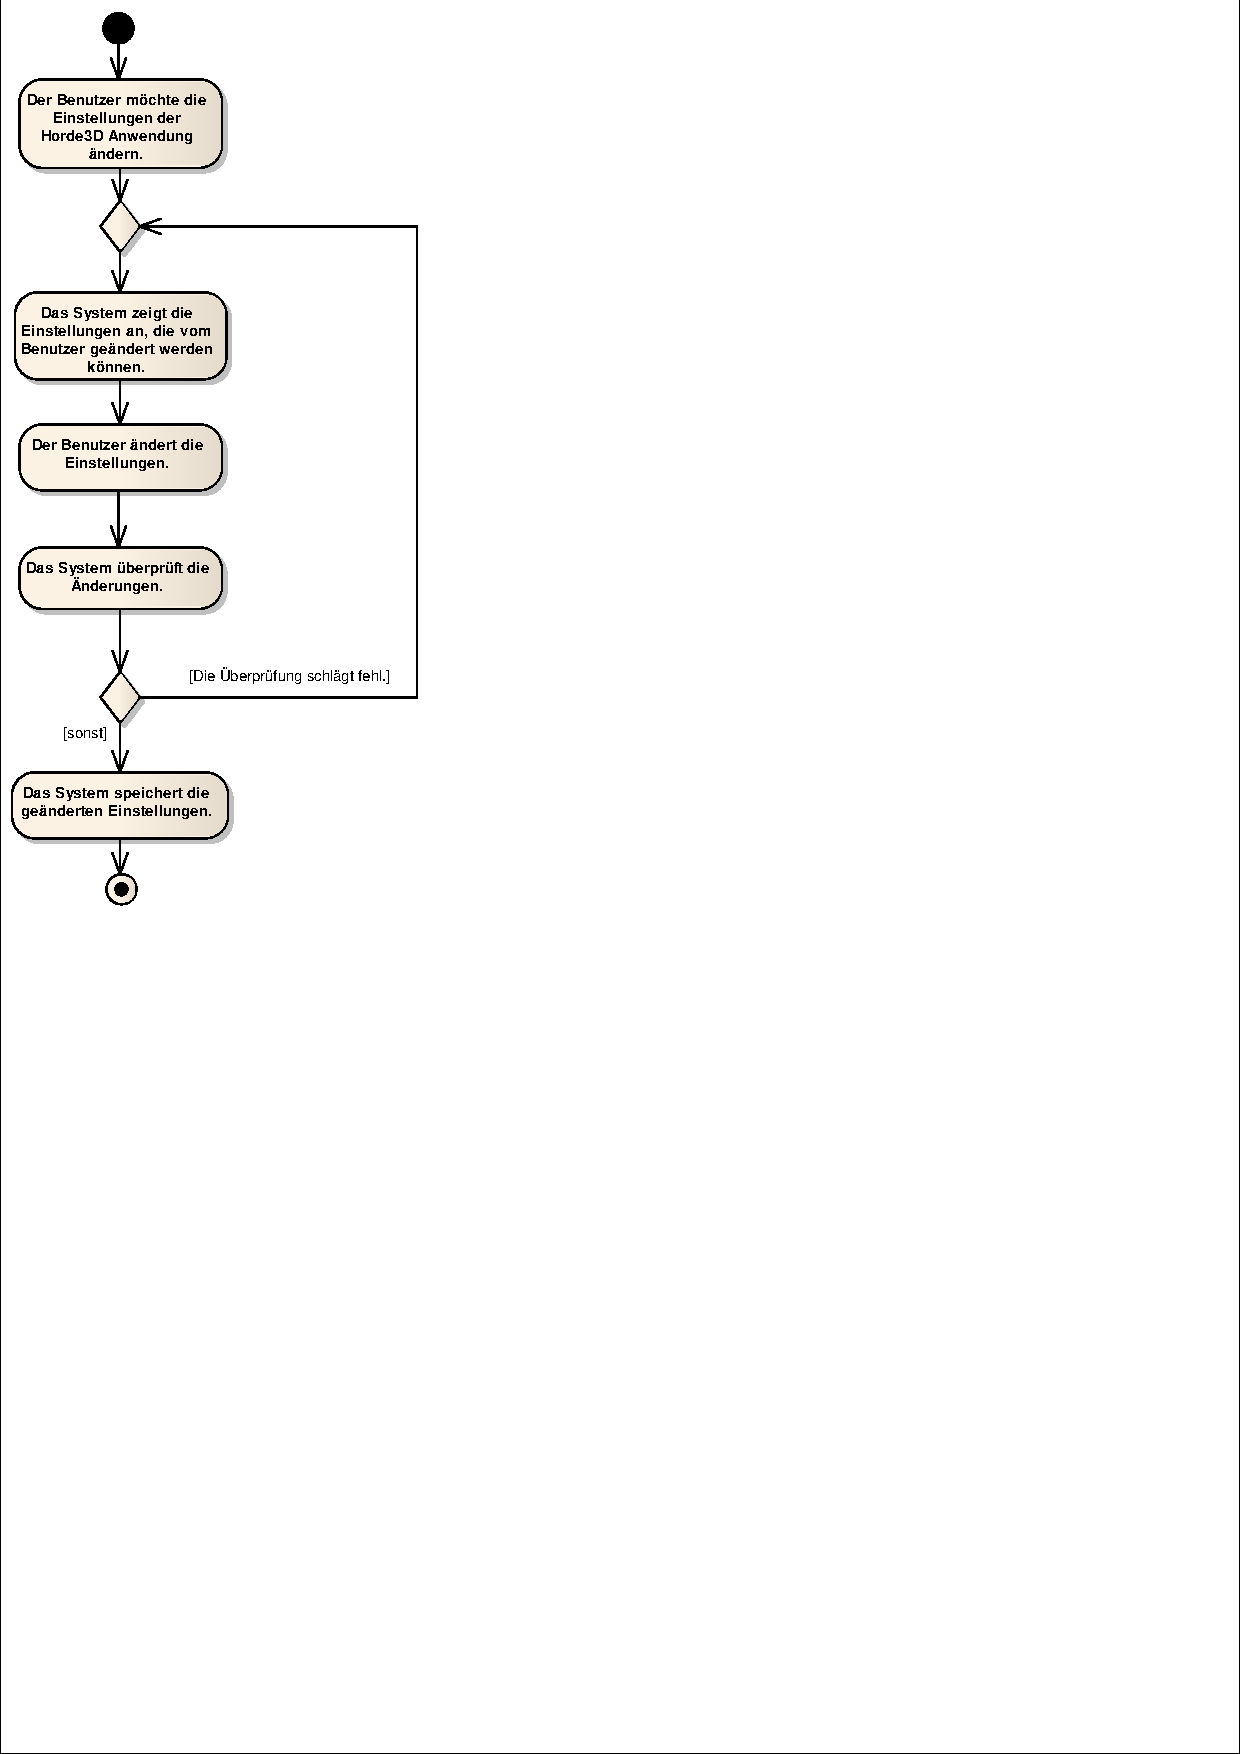
\includegraphics[trim = 1mm 140mm 135mm 1mm, clip, scale=0.7]{images/UseCase_EinstellungenAendern.pdf}
\caption{Aktivit�tsdiagramm f�r den Anwendungsfall "`Einstellungen �ndern"'}\label{fig:ucEinstellungenAendern}
\end{figure}

\begin{figure}[htp]
\centering
%trim=l b r t  	This option will crop the imported image by l from the left, b from the bottom, r from the right, and t  from the top. Where l, b, r and t are lengths. 
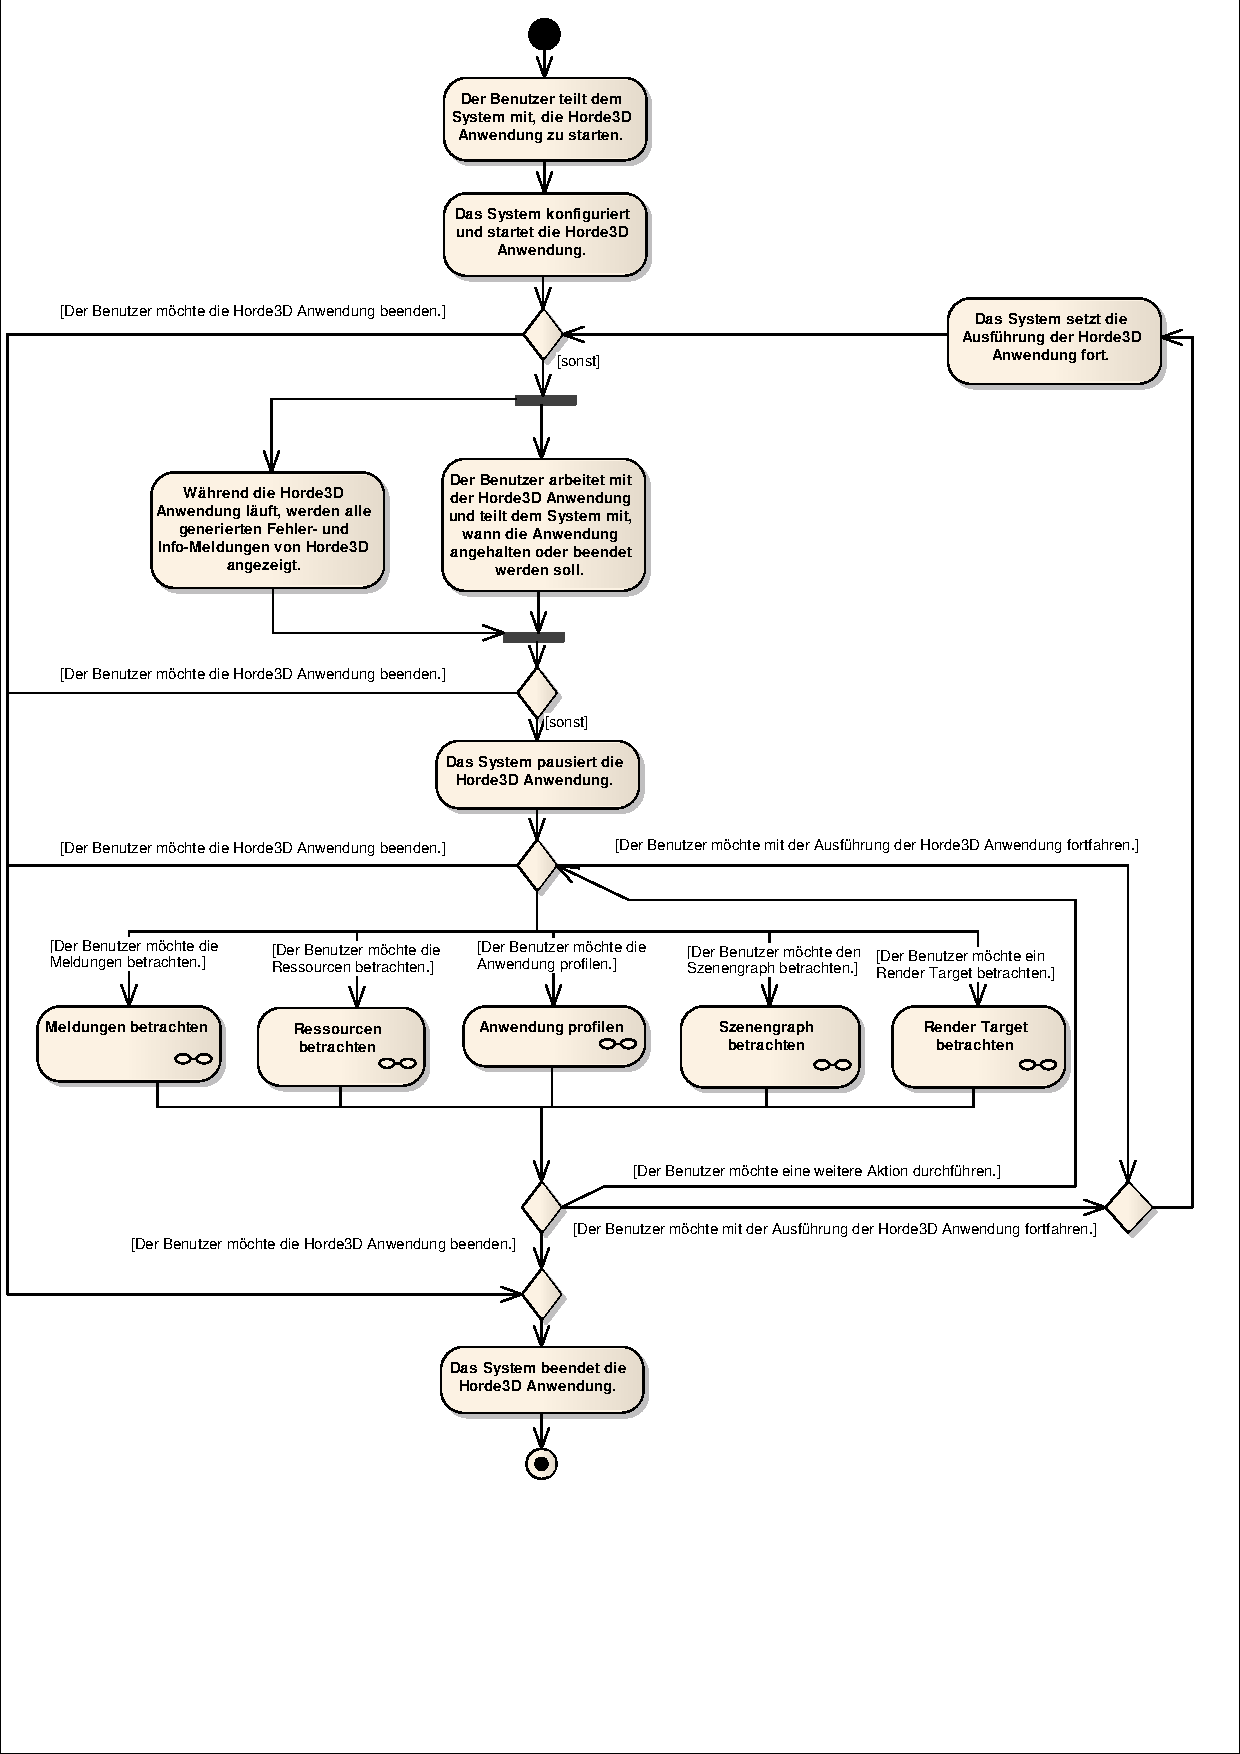
\includegraphics[trim = 1mm 45mm 5mm 1mm, clip, scale=0.7]{images/UseCase_AnwendungAusfuehren.pdf}
\caption{Aktivit�tsdiagramm f�r den Anwendungsfall "`Anwendung ausf�hren"'}\label{fig:ucAnwendungAusfuehren}
\end{figure}

\begin{figure}[ht]
\centering
%trim=l b r t  	This option will crop the imported image by l from the left, b from the bottom, r from the right, and t  from the top. Where l, b, r and t are lengths. 
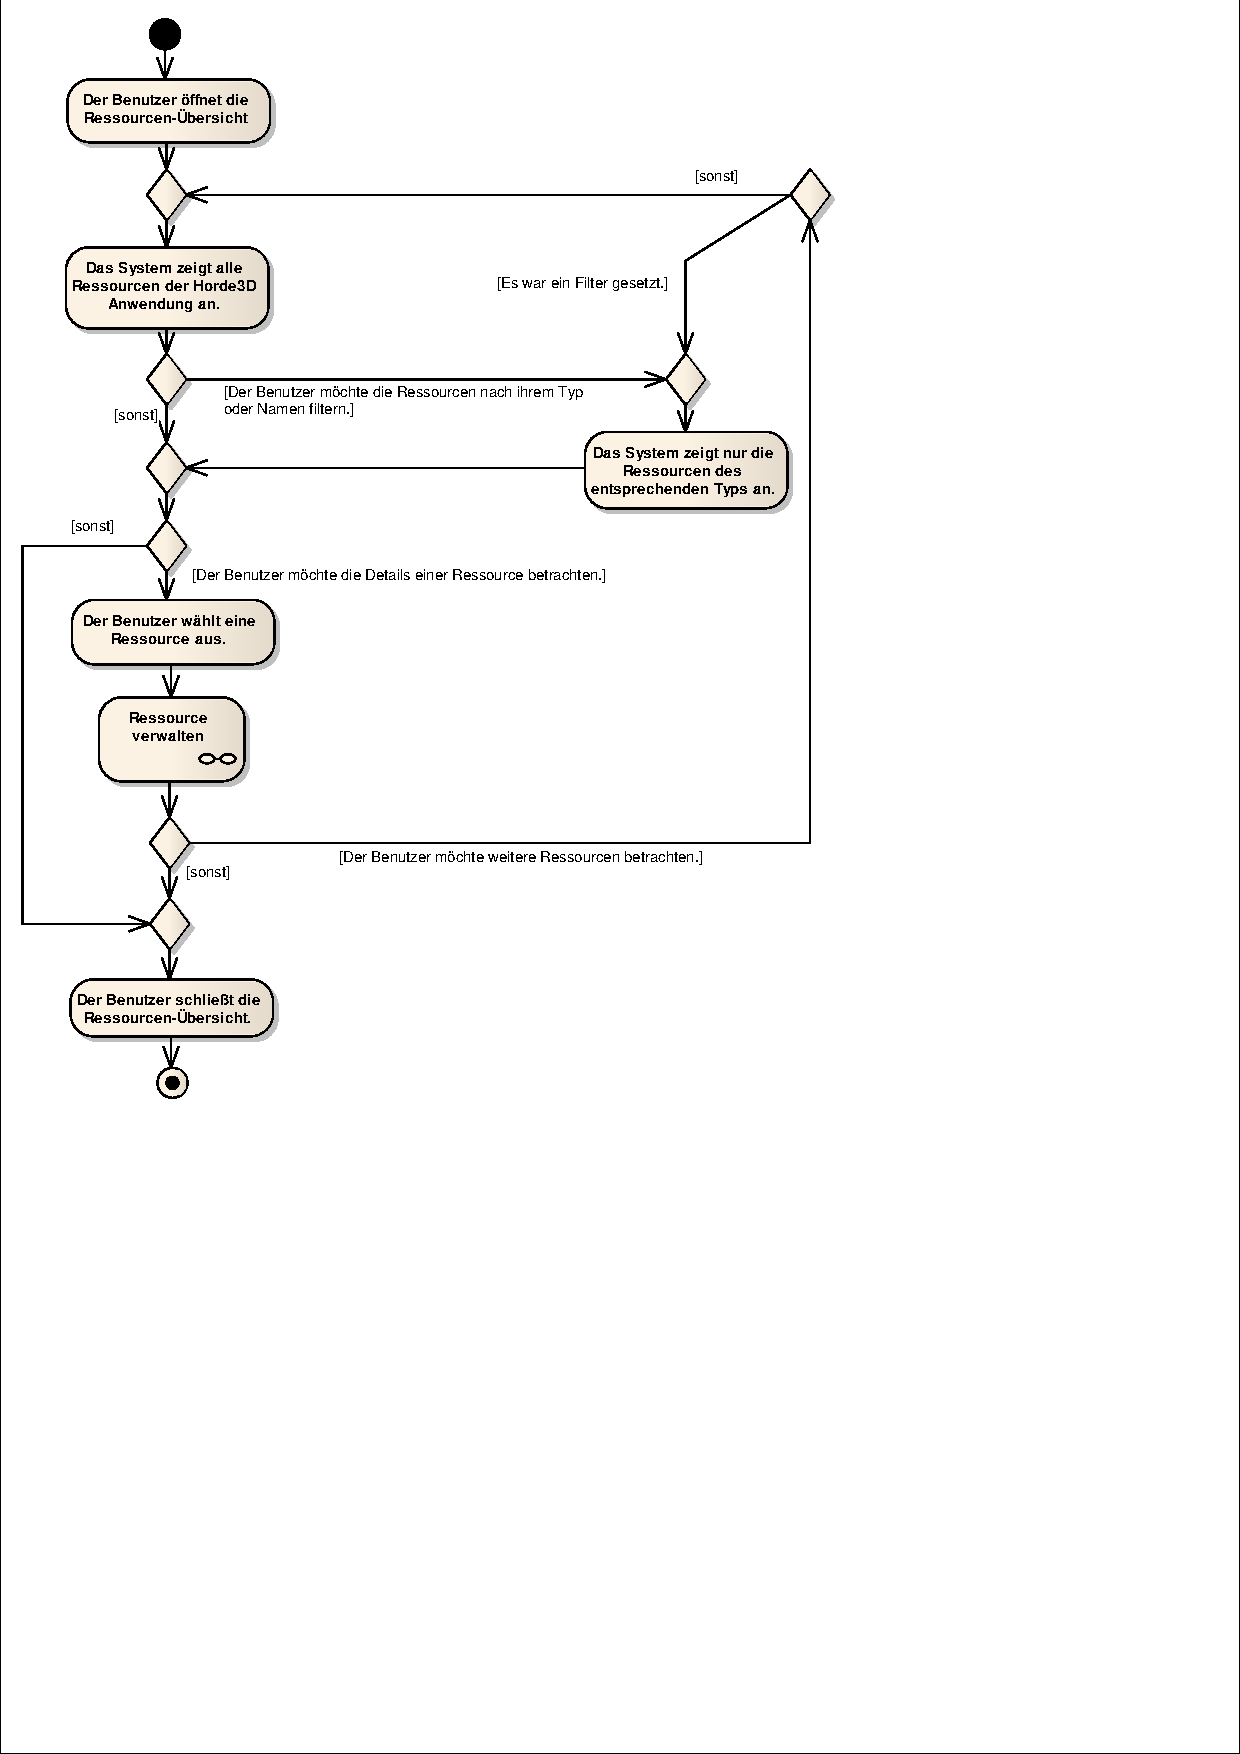
\includegraphics[trim = 1mm 110mm 60mm 1mm, clip, scale=0.7]{images/UseCase_RessourcenBetrachten.pdf}
\caption{Aktivit�tsdiagramm f�r den Anwendungsfall "`Ressourcen betrachten"'}\label{fig:ucRessourcenBetrachten}
\end{figure}

\begin{figure}[ht]
\centering
%trim=l b r t  	This option will crop the imported image by l from the left, b from the bottom, r from the right, and t  from the top. Where l, b, r and t are lengths. 
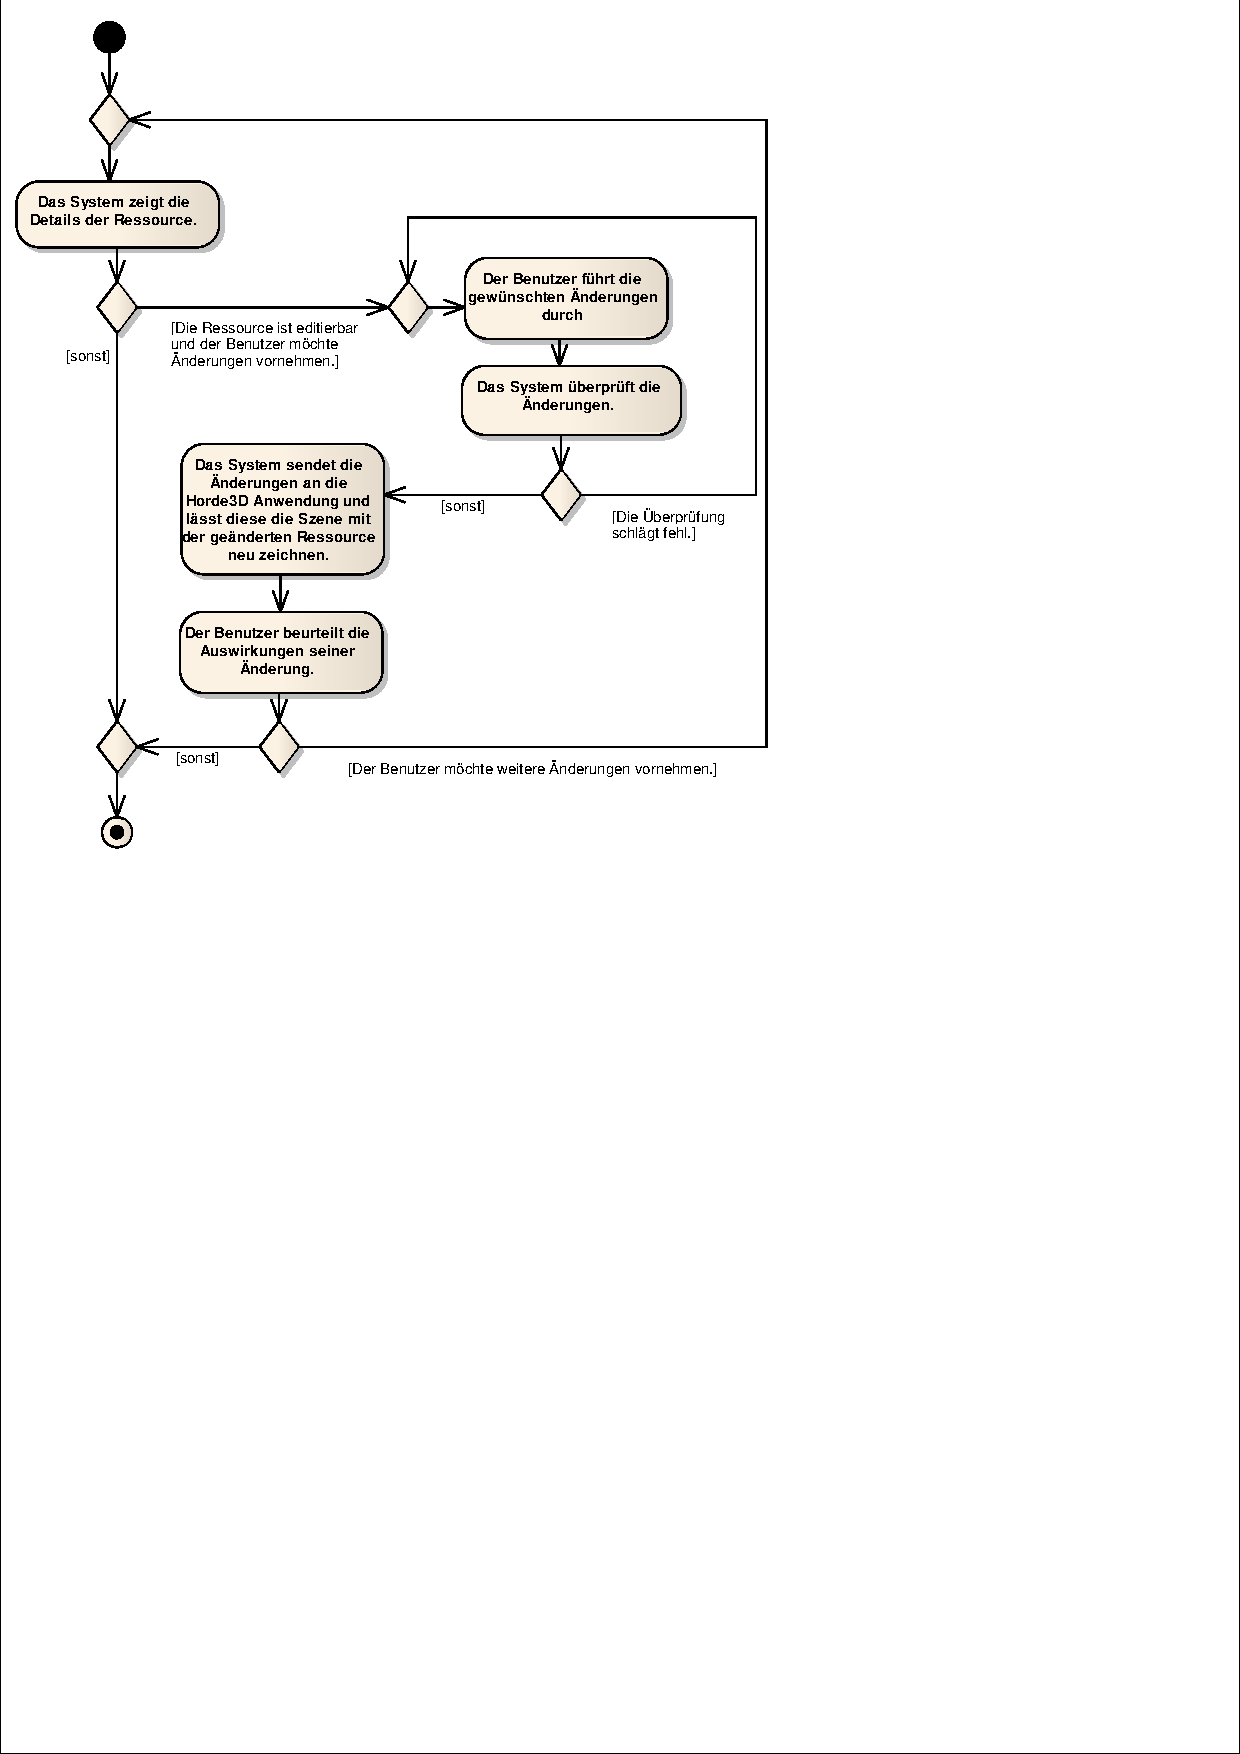
\includegraphics[trim = 1mm 150mm 80mm 1mm, clip, scale=0.7]{images/UseCase_RessourceVerwalten.pdf}
\caption{Aktivit�tsdiagramm f�r den Anwendungsfall "`Ressource verwalten"'}\label{fig:ucRessourceVerwalten}
\end{figure}

\begin{figure}[htp]
\centering
%trim=l b r t  	This option will crop the imported image by l from the left, b from the bottom, r from the right, and t  from the top. Where l, b, r and t are lengths. 
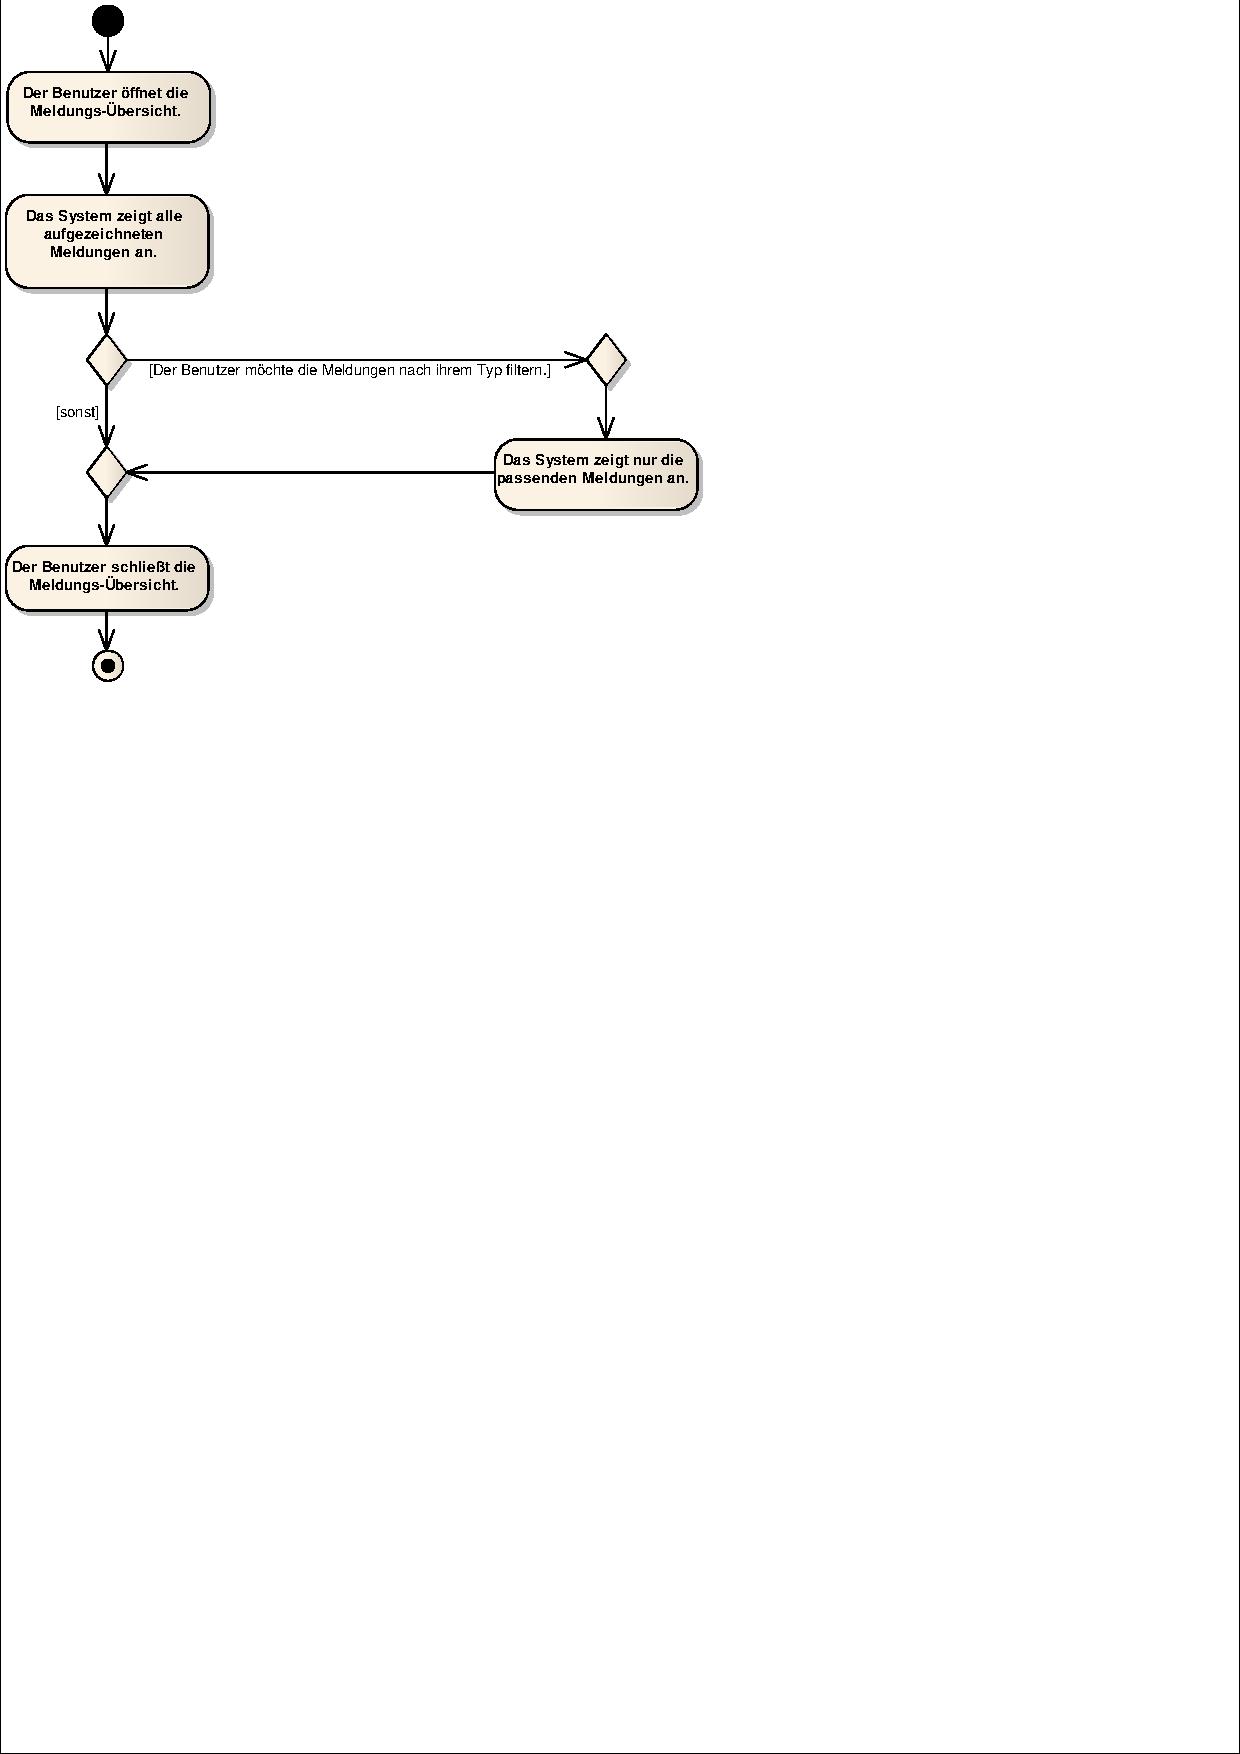
\includegraphics[trim = 1mm 180mm 90mm 1mm, clip, scale=0.7]{images/UseCase_MeldungenBetrachten.pdf}
\caption{Aktivit�tsdiagramm f�r den Anwendungsfall "`Meldungen betrachten"'}\label{fig:ucMeldungenBetrachten}
\end{figure}

\begin{figure}[htp]
\centering
%trim=l b r t  	This option will crop the imported image by l from the left, b from the bottom, r from the right, and t  from the top. Where l, b, r and t are lengths. 
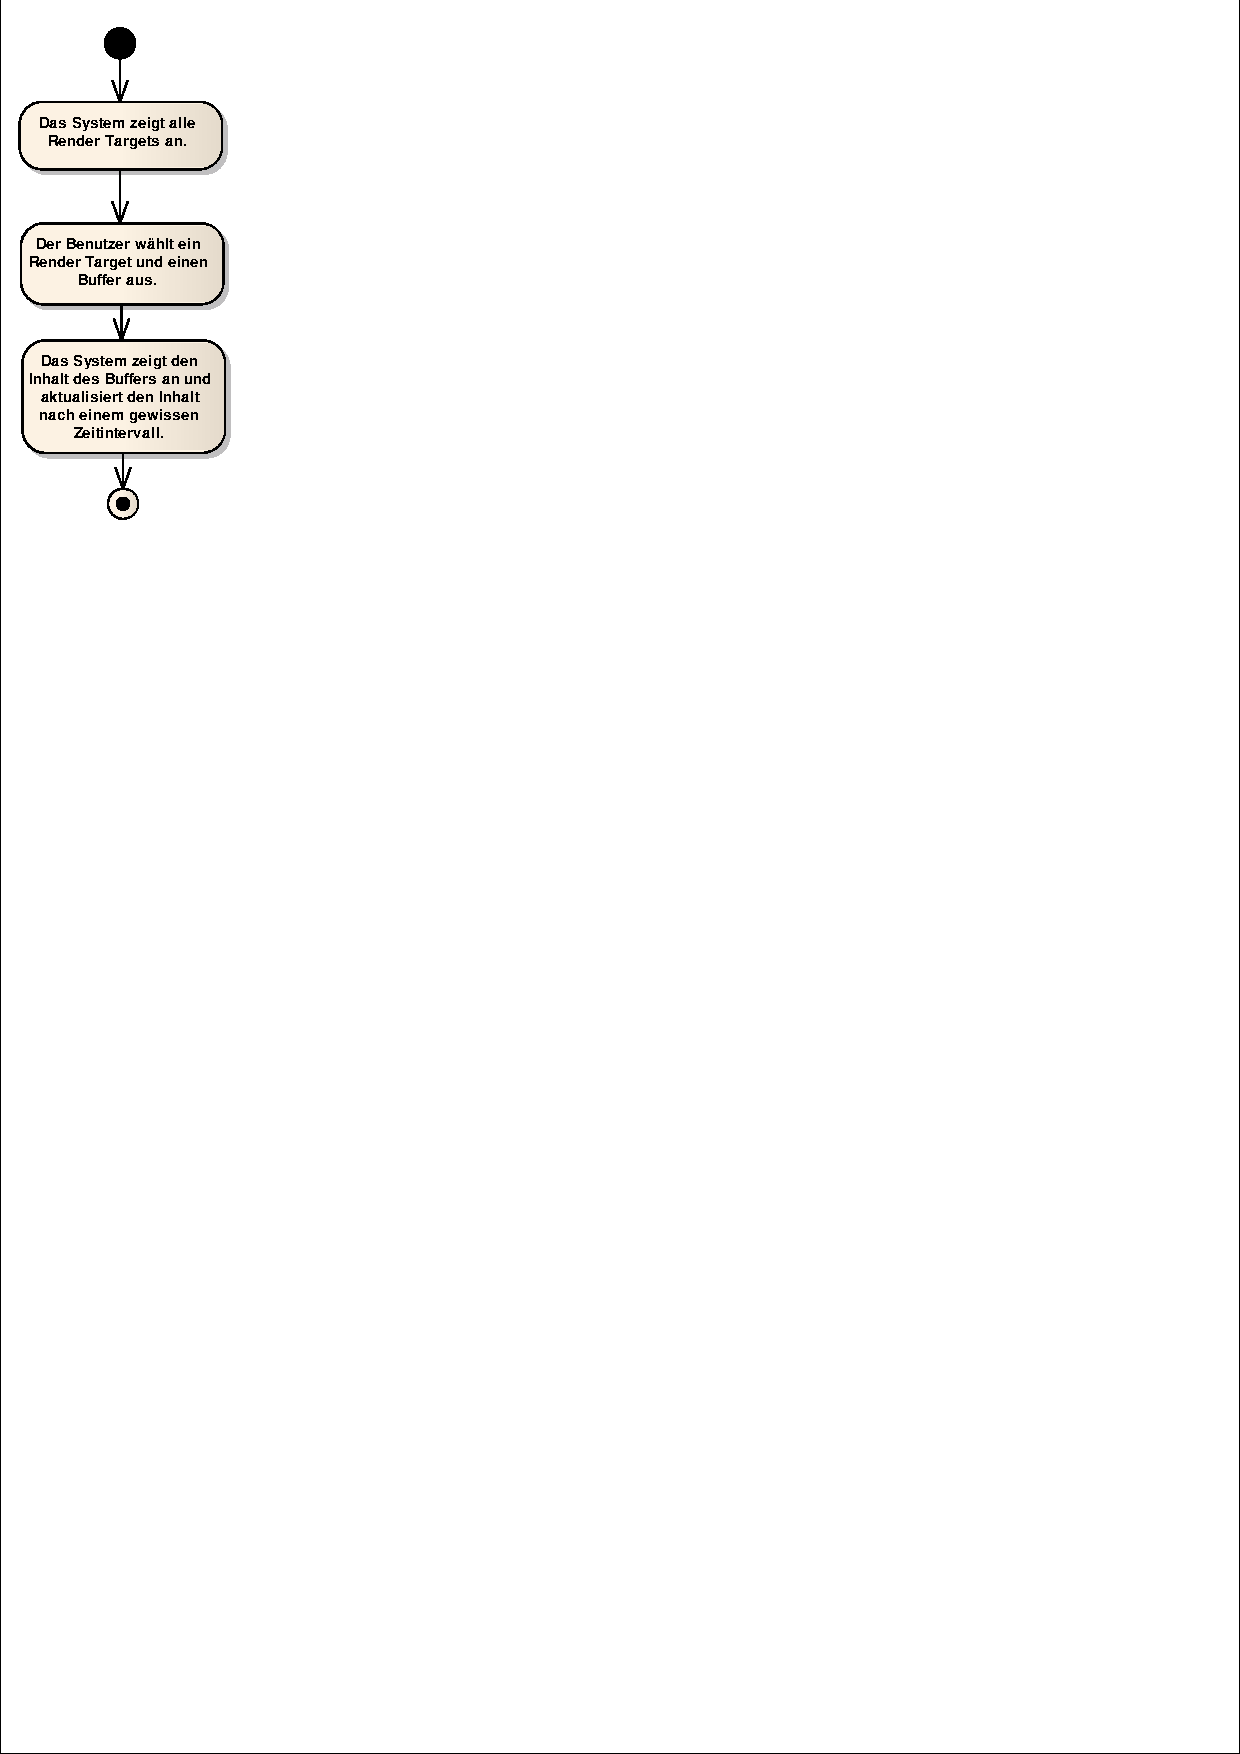
\includegraphics[trim = 1mm 205mm 150mm 1mm, clip, scale=0.7]{images/UseCase_RenderTargetBetrachten.pdf}
\caption{Aktivit�tsdiagramm f�r den Anwendungsfall "`Render Target betrachten"'}\label{fig:ucRenderTargetBetrachten}
\end{figure}

\begin{figure}[htp]
\centering
%trim=l b r t  	This option will crop the imported image by l from the left, b from the bottom, r from the right, and t  from the top. Where l, b, r and t are lengths. 
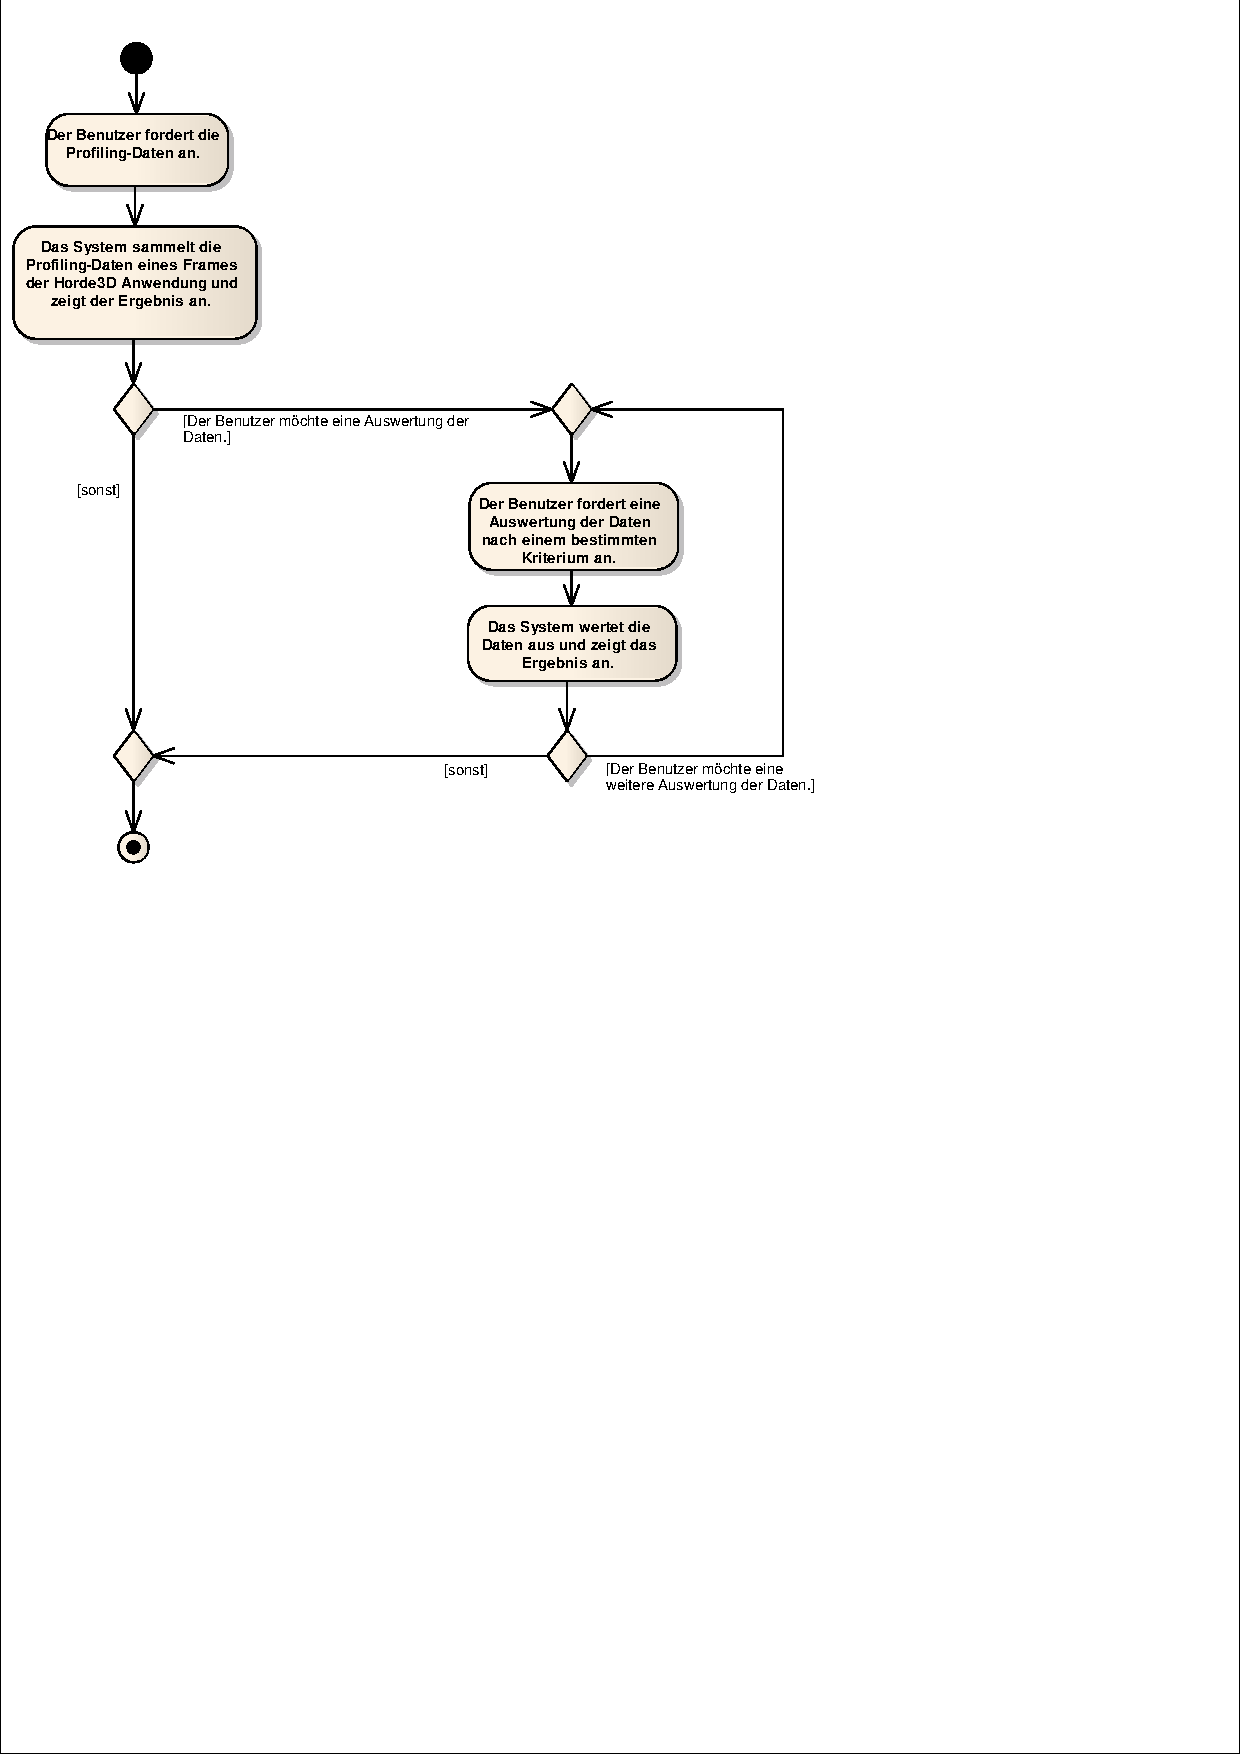
\includegraphics[trim = 1mm 150mm 60mm 1mm, clip, scale=0.7]{images/UseCase_AnwendungProfilen.pdf}
\caption{Aktivit�tsdiagramm f�r den Anwendungsfall "`Anwendung profilen"'}\label{fig:ucAnwendungProfilen}
\end{figure}

\begin{figure}[htp]
\centering
%trim=l b r t  	This option will crop the imported image by l from the left, b from the bottom, r from the right, and t  from the top. Where l, b, r and t are lengths. 
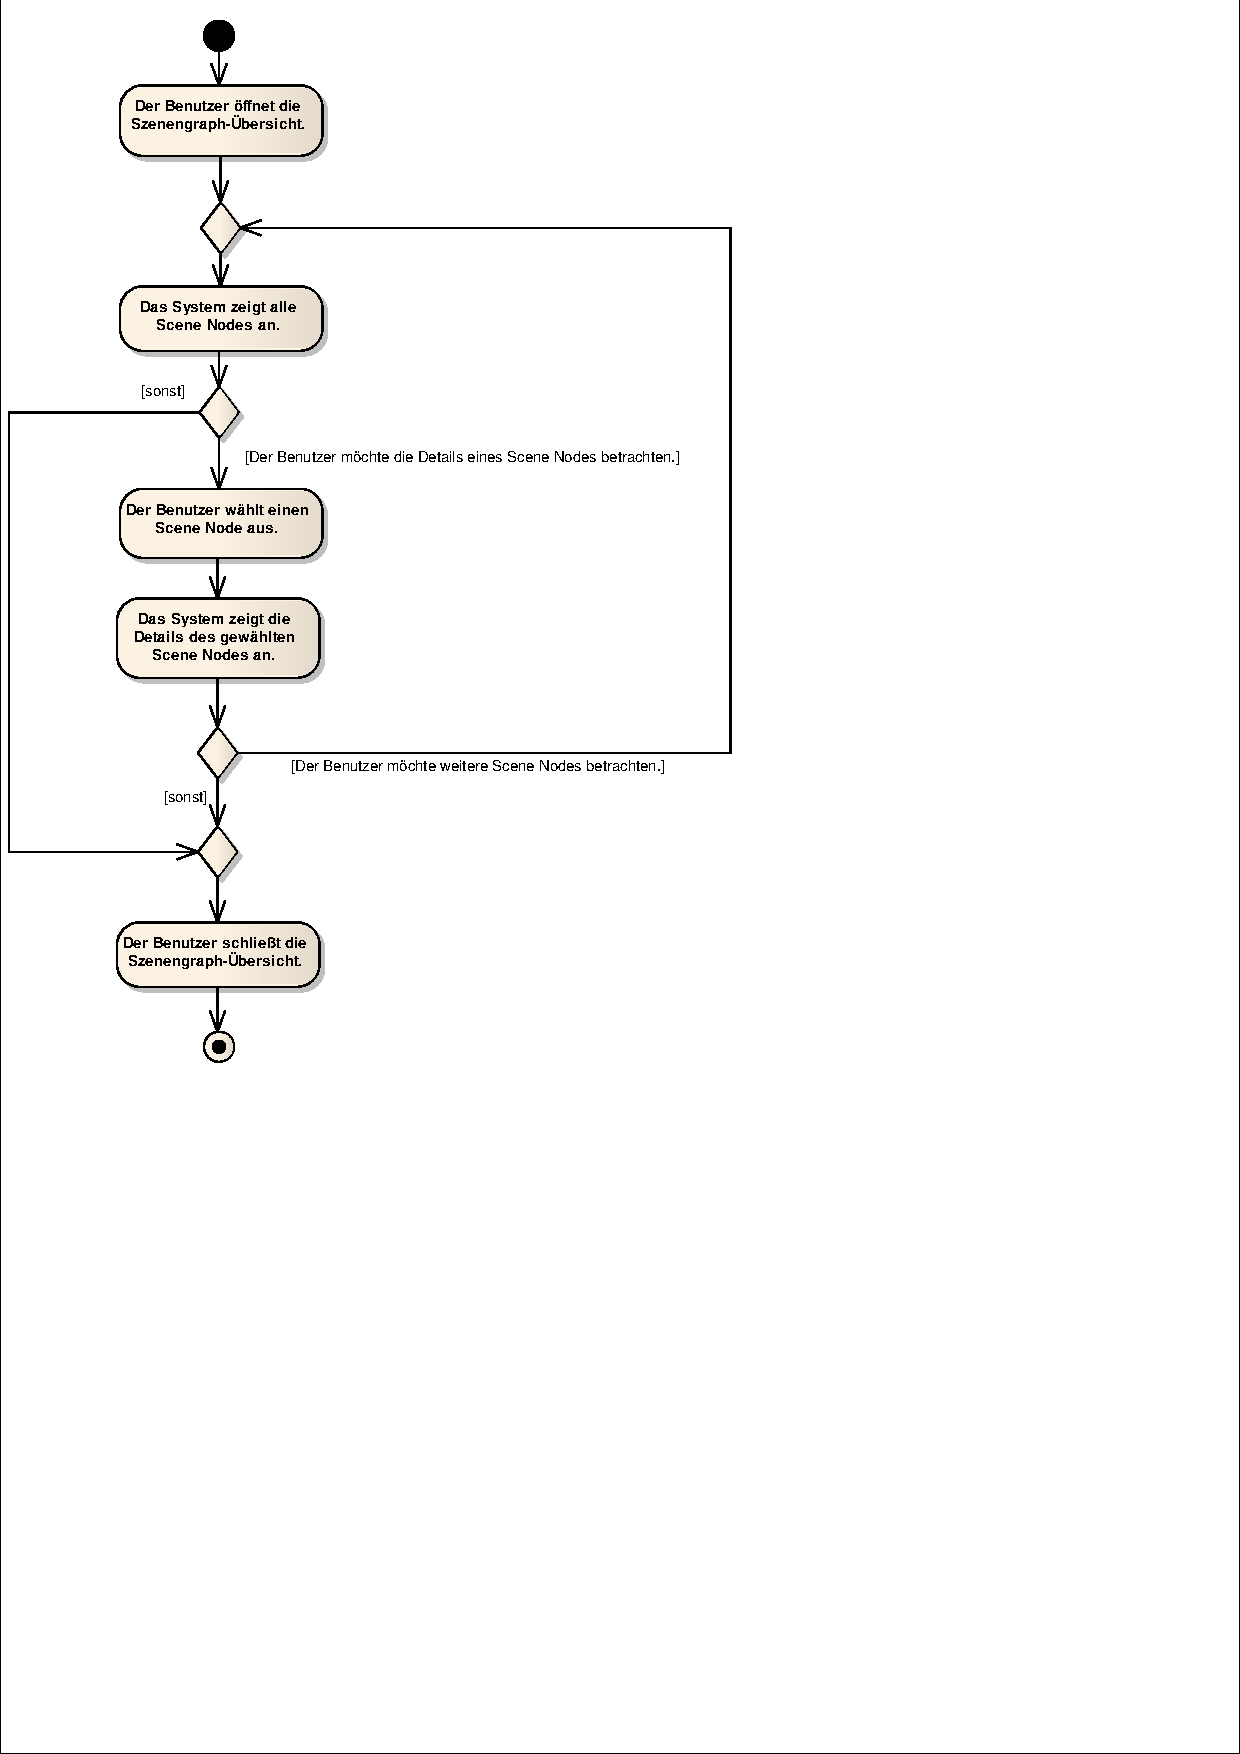
\includegraphics[trim = 1mm 115mm 70mm 1mm, clip, scale=0.7]{images/UseCase_SzenengraphBetrachten.pdf}
\caption{Aktivit�tsdiagramm f�r den Anwendungsfall "`Szenengraph betrachten"'}\label{fig:ucSzenengraphBetrachten}
\end{figure}

\begin{figure}[htp]
\centering
%trim=l b r t  	This option will crop the imported image by l from the left, b from the bottom, r from the right, and t  from the top. Where l, b, r and t are lengths. 
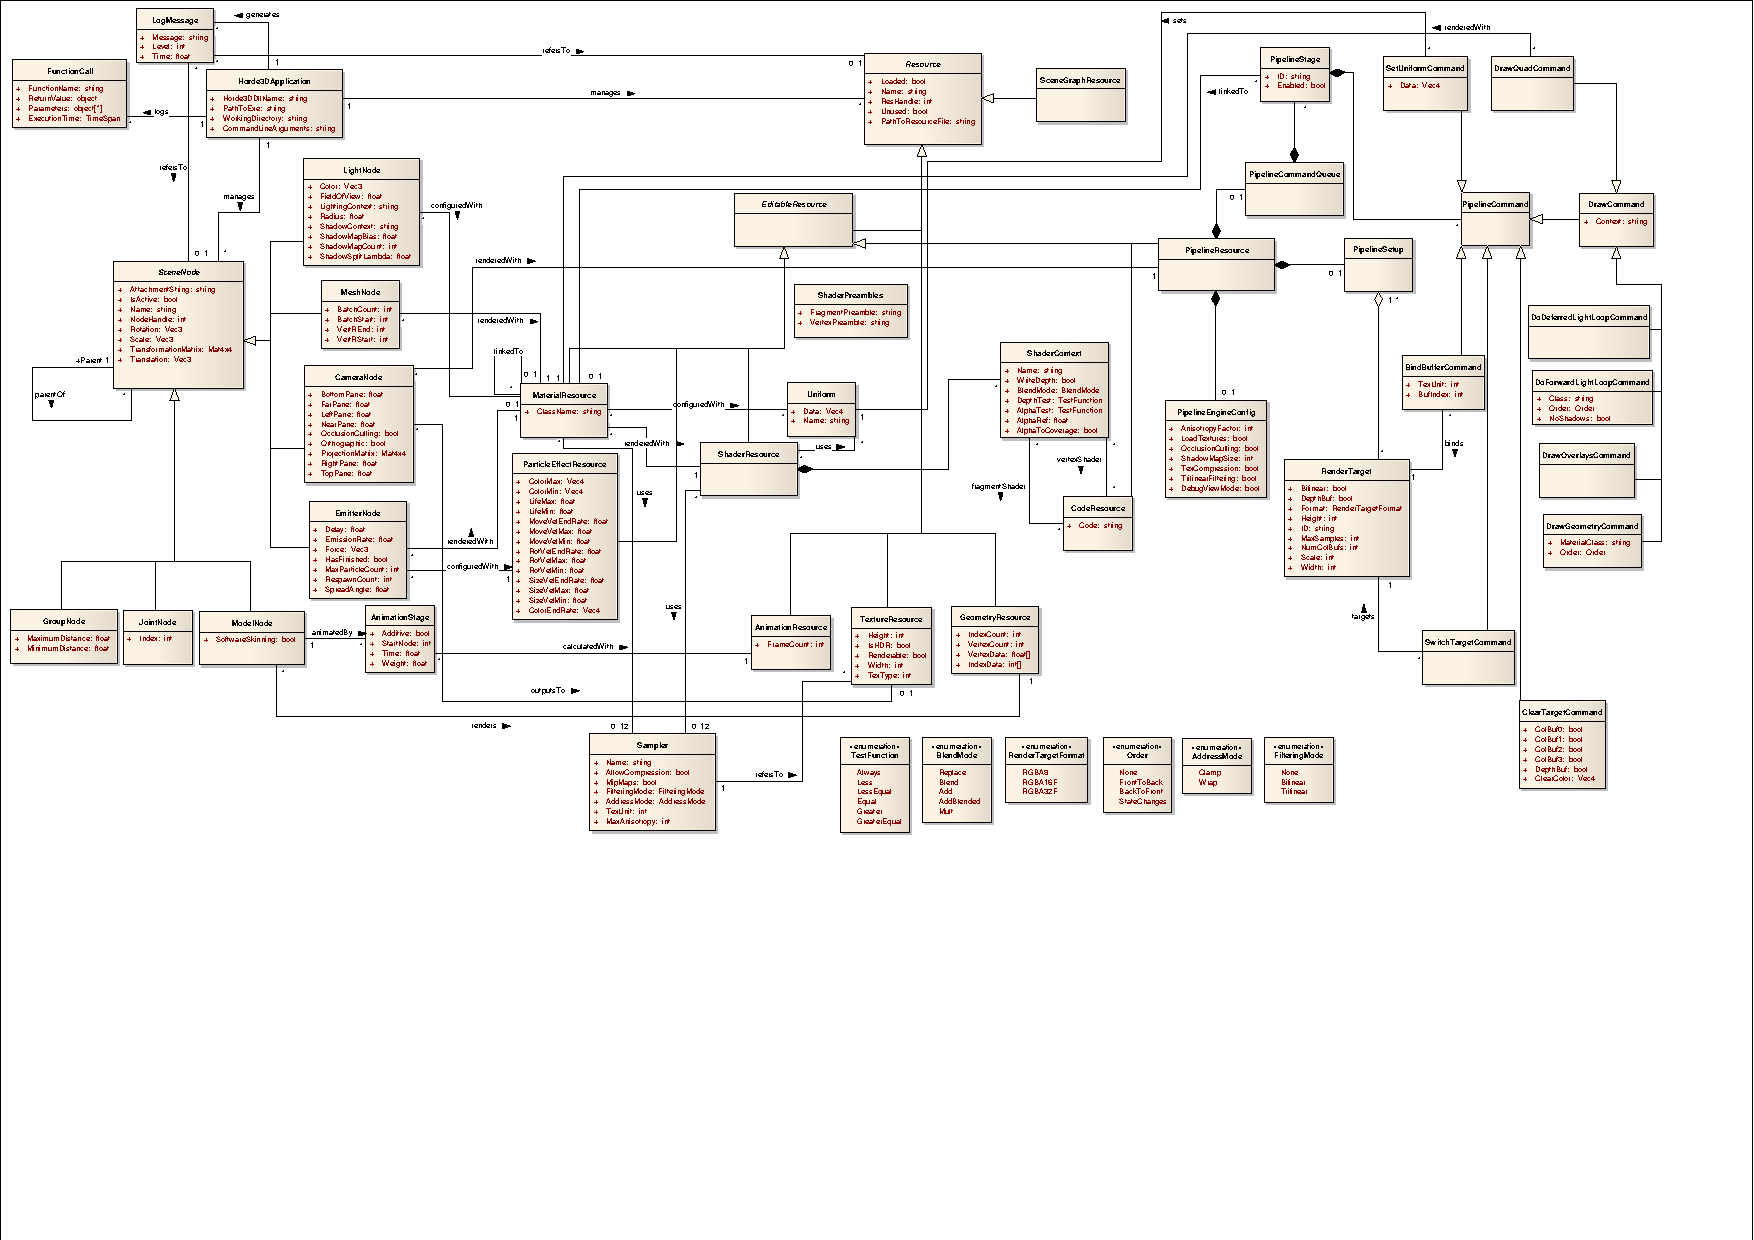
\includegraphics[trim = 1mm 65mm 15mm 1mm, clip, scale = 0.75, angle = 90]{images/DomainModel.pdf}
\caption{Das Konzeptmodell des \DevEnvs}\label{fig:domainModel}
\end{figure}

\chapter{Artefakte der Design-Phase}

\begin{figure}[htp]
\centering
%trim=l b r t  	This option will crop the imported image by l from the left, b from the bottom, r from the right, and t  from the top. Where l, b, r and t are lengths. 
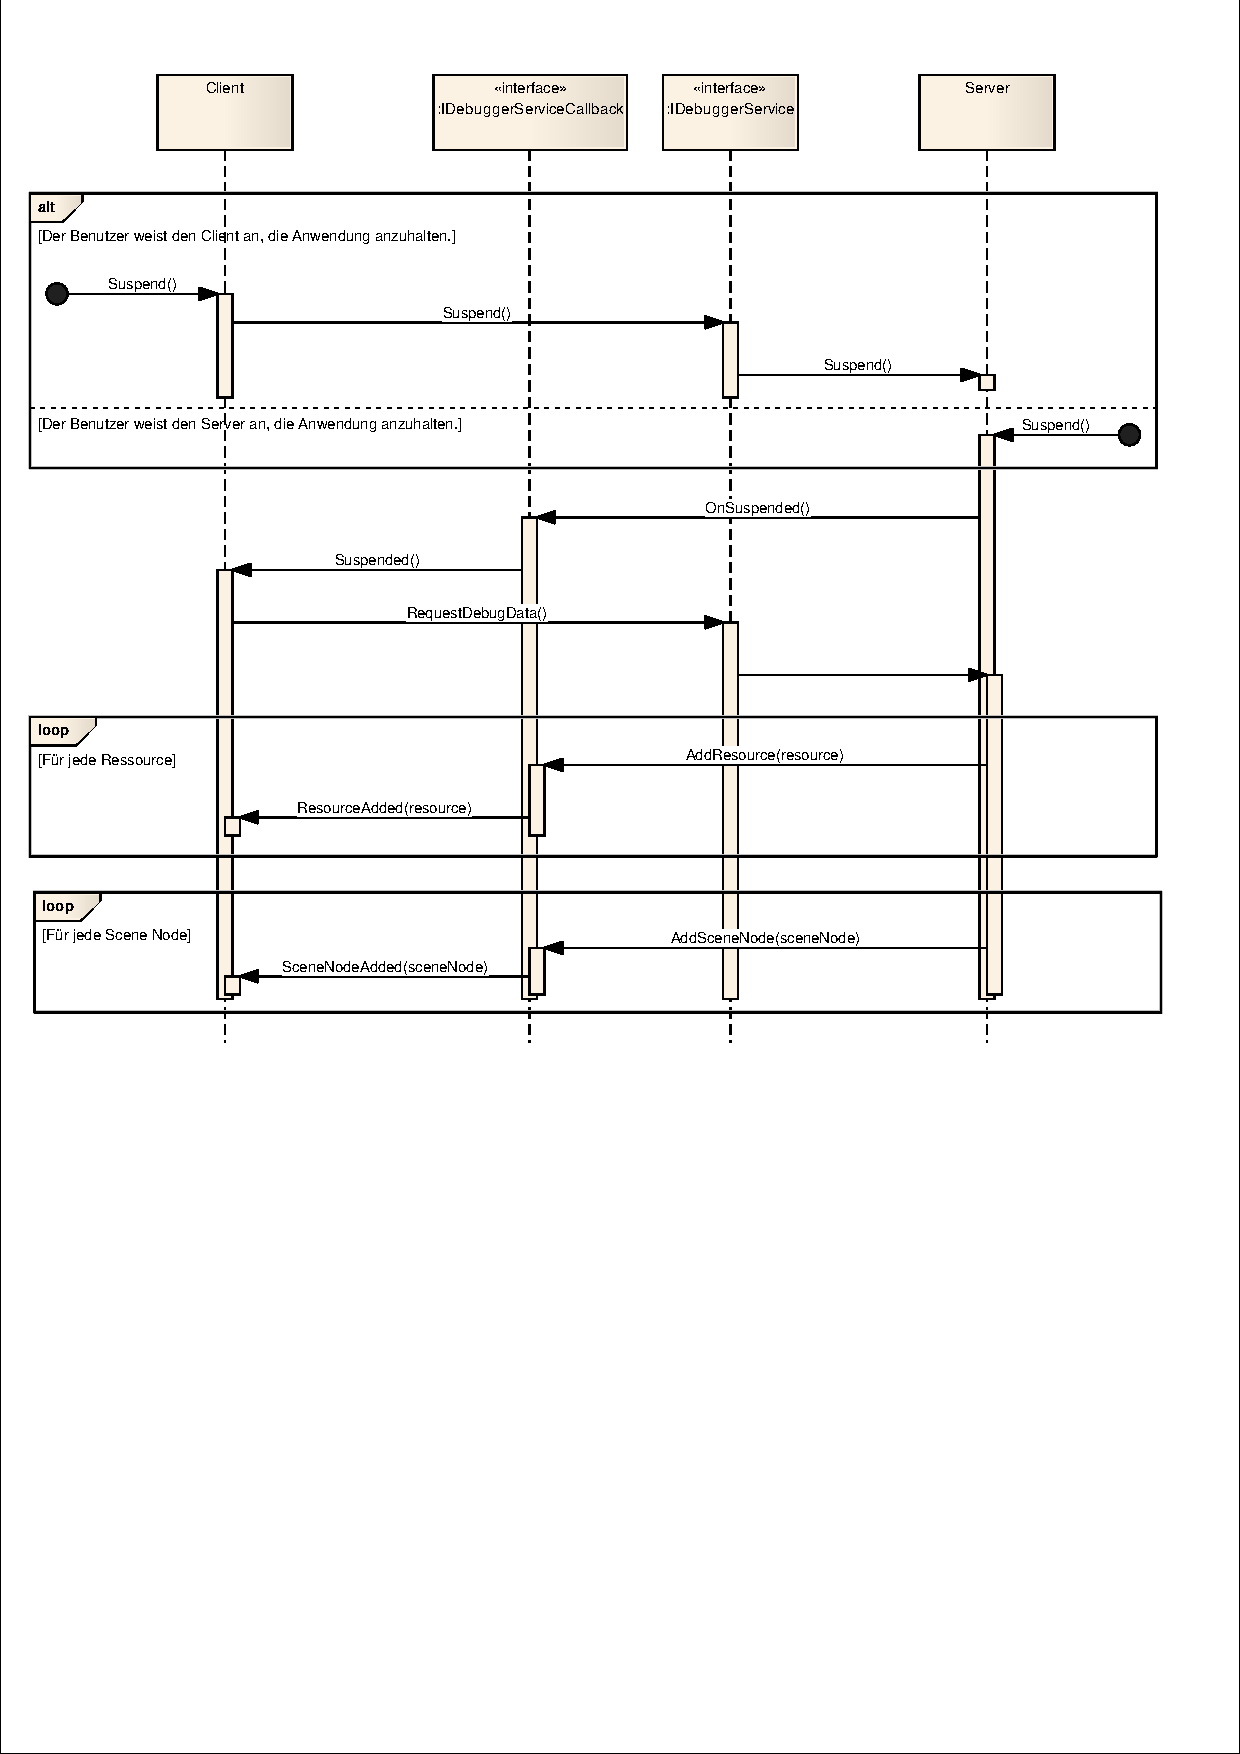
\includegraphics[trim = 5mm 120mm 5mm 10mm, clip,scale=0.7]{images/ClientServerCommunication.pdf}
\caption{Sequenzdiagramm f�r die Client-Server-Interaktionen beim Anhalten der Anwendung}\label{fig:ClientServerCommunication}
\end{figure}

\begin{figure}[htp]
\centering
%trim=l b r t  	This option will crop the imported image by l from the left, b from the bottom, r from the right, and t  from the top. Where l, b, r and t are lengths. 
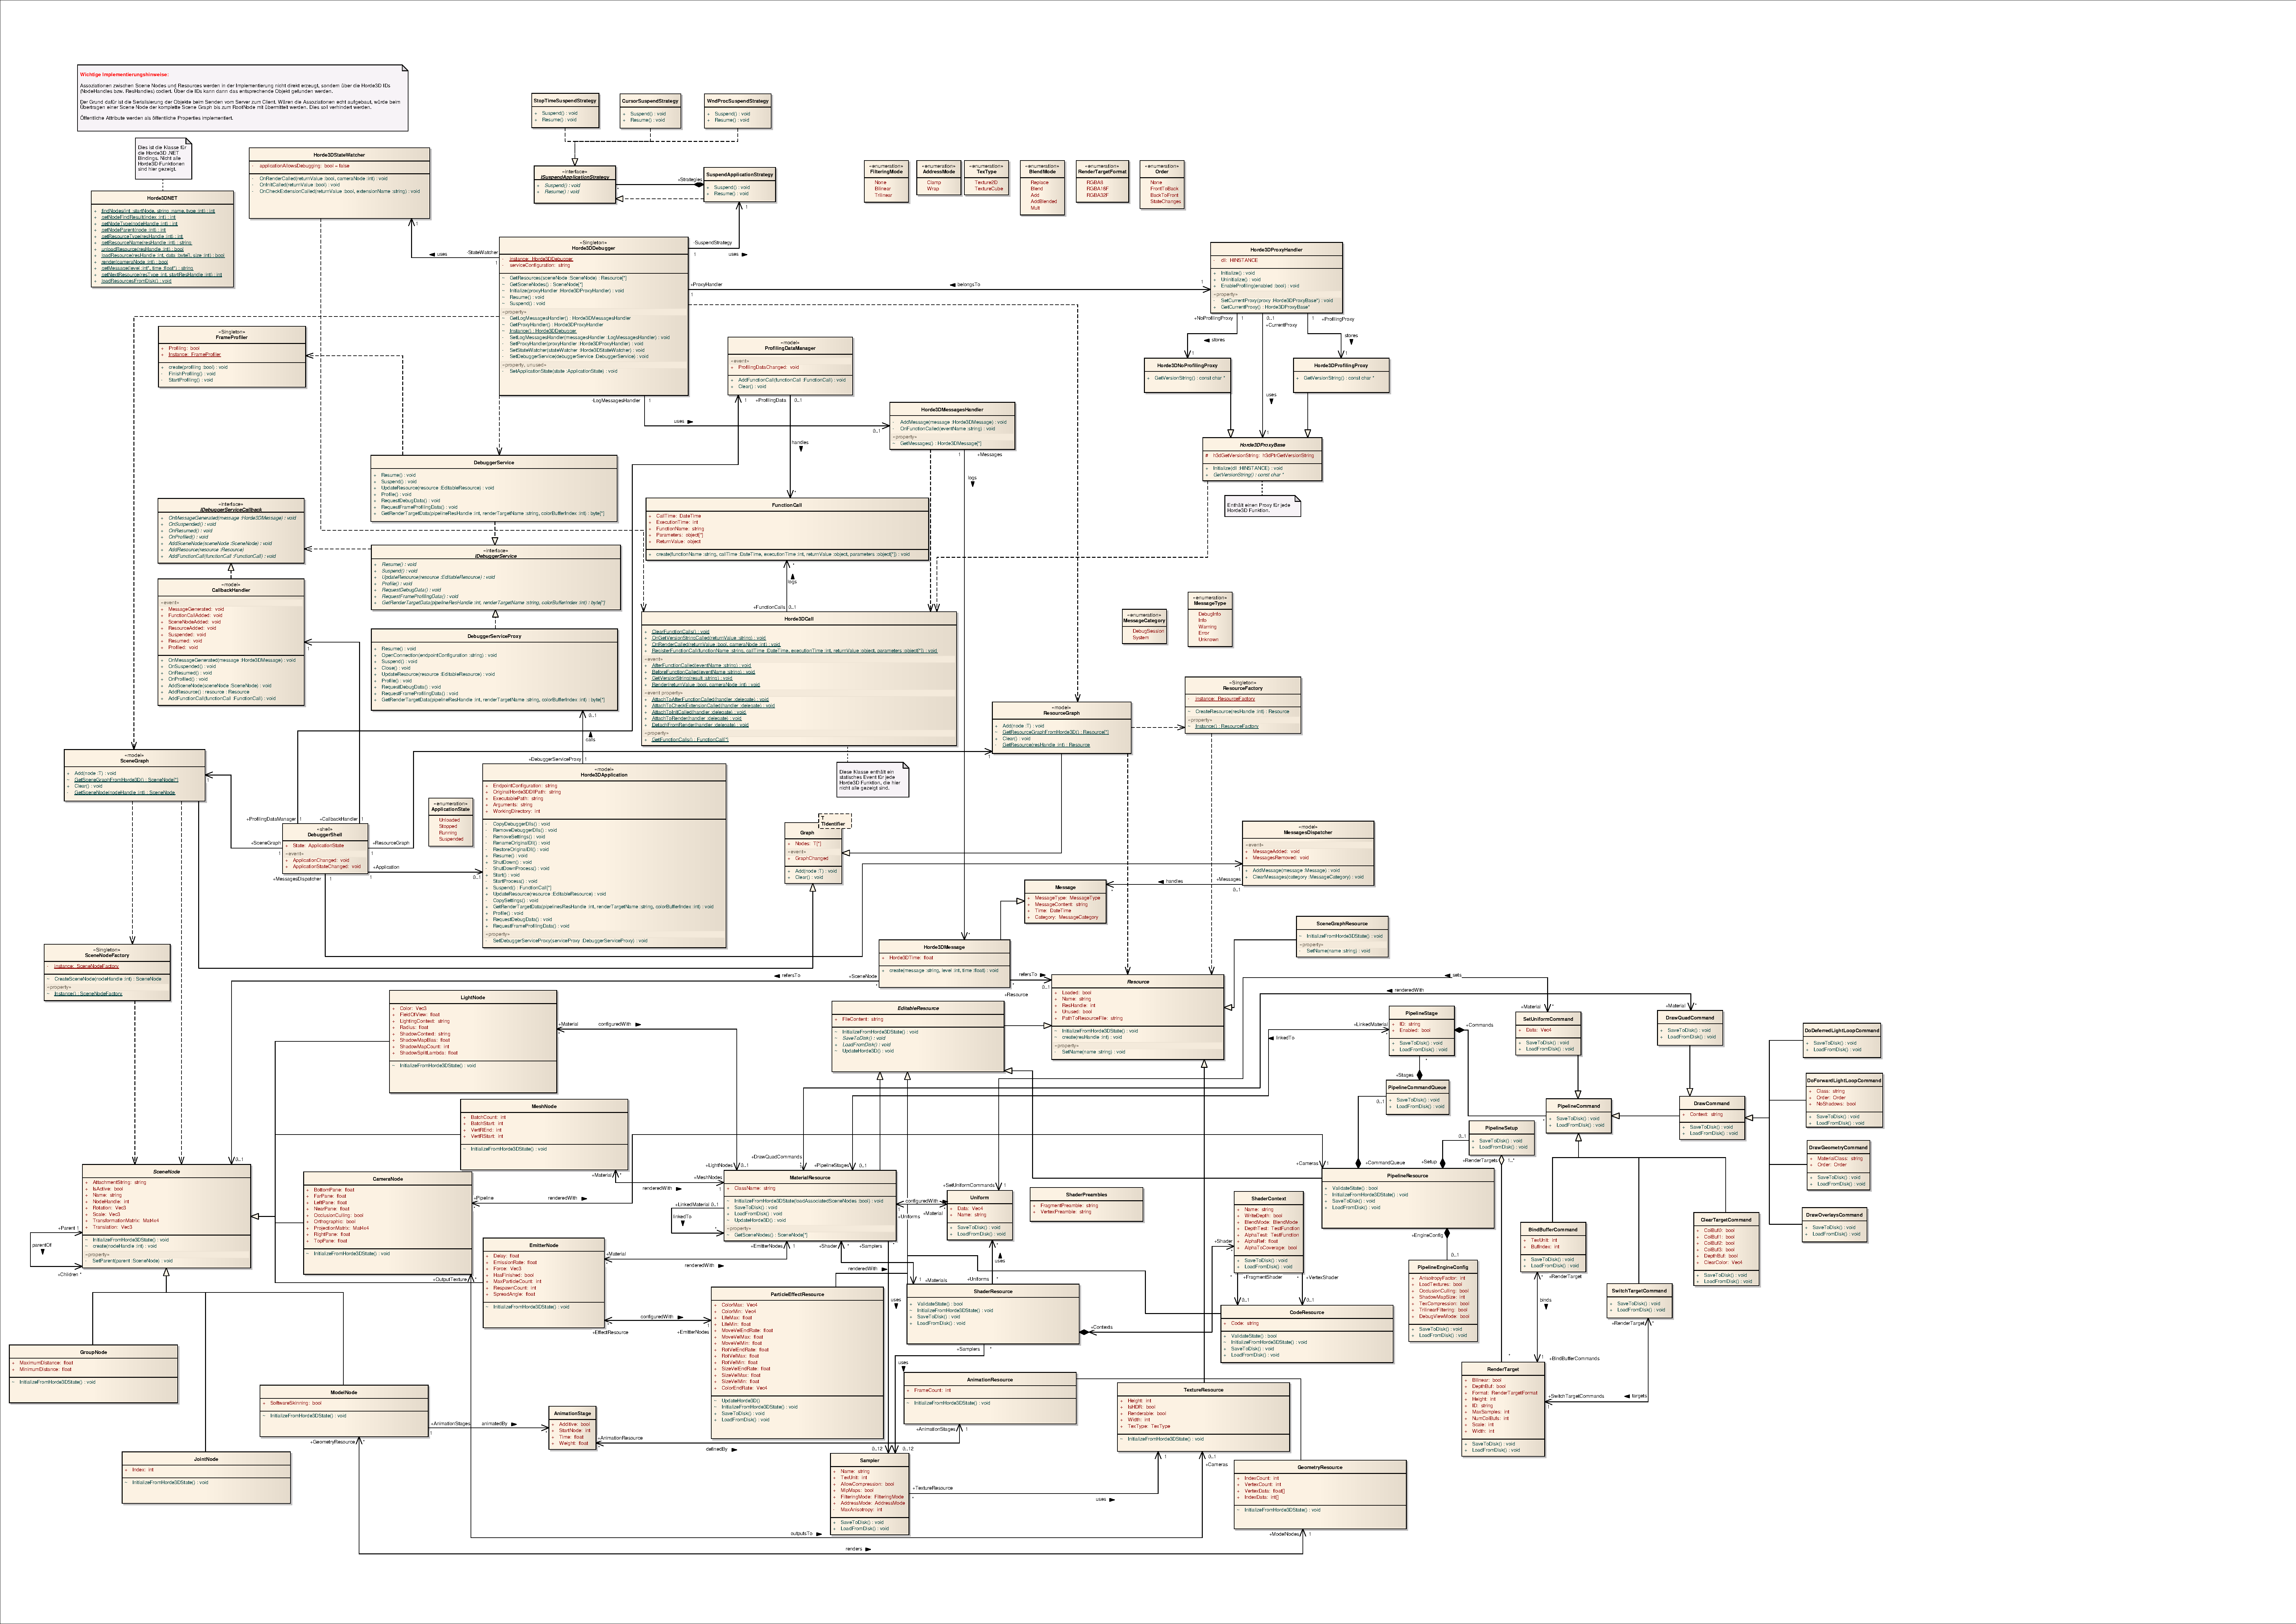
\includegraphics[trim = 70mm 468mm 865mm 230mm, clip, angle = 90, scale=0.7]{images/Designmodell.pdf}
\caption{Ausschnitt aus dem Designmodell f�r die Client-Server-Schnittstelle}\label{fig:clientServerInterfaceDesign}
\end{figure}

\begin{figure}[htp]
\centering
%trim=l b r t  	This option will crop the imported image by l from the left, b from the bottom, r from the right, and t  from the top. Where l, b, r and t are lengths. 
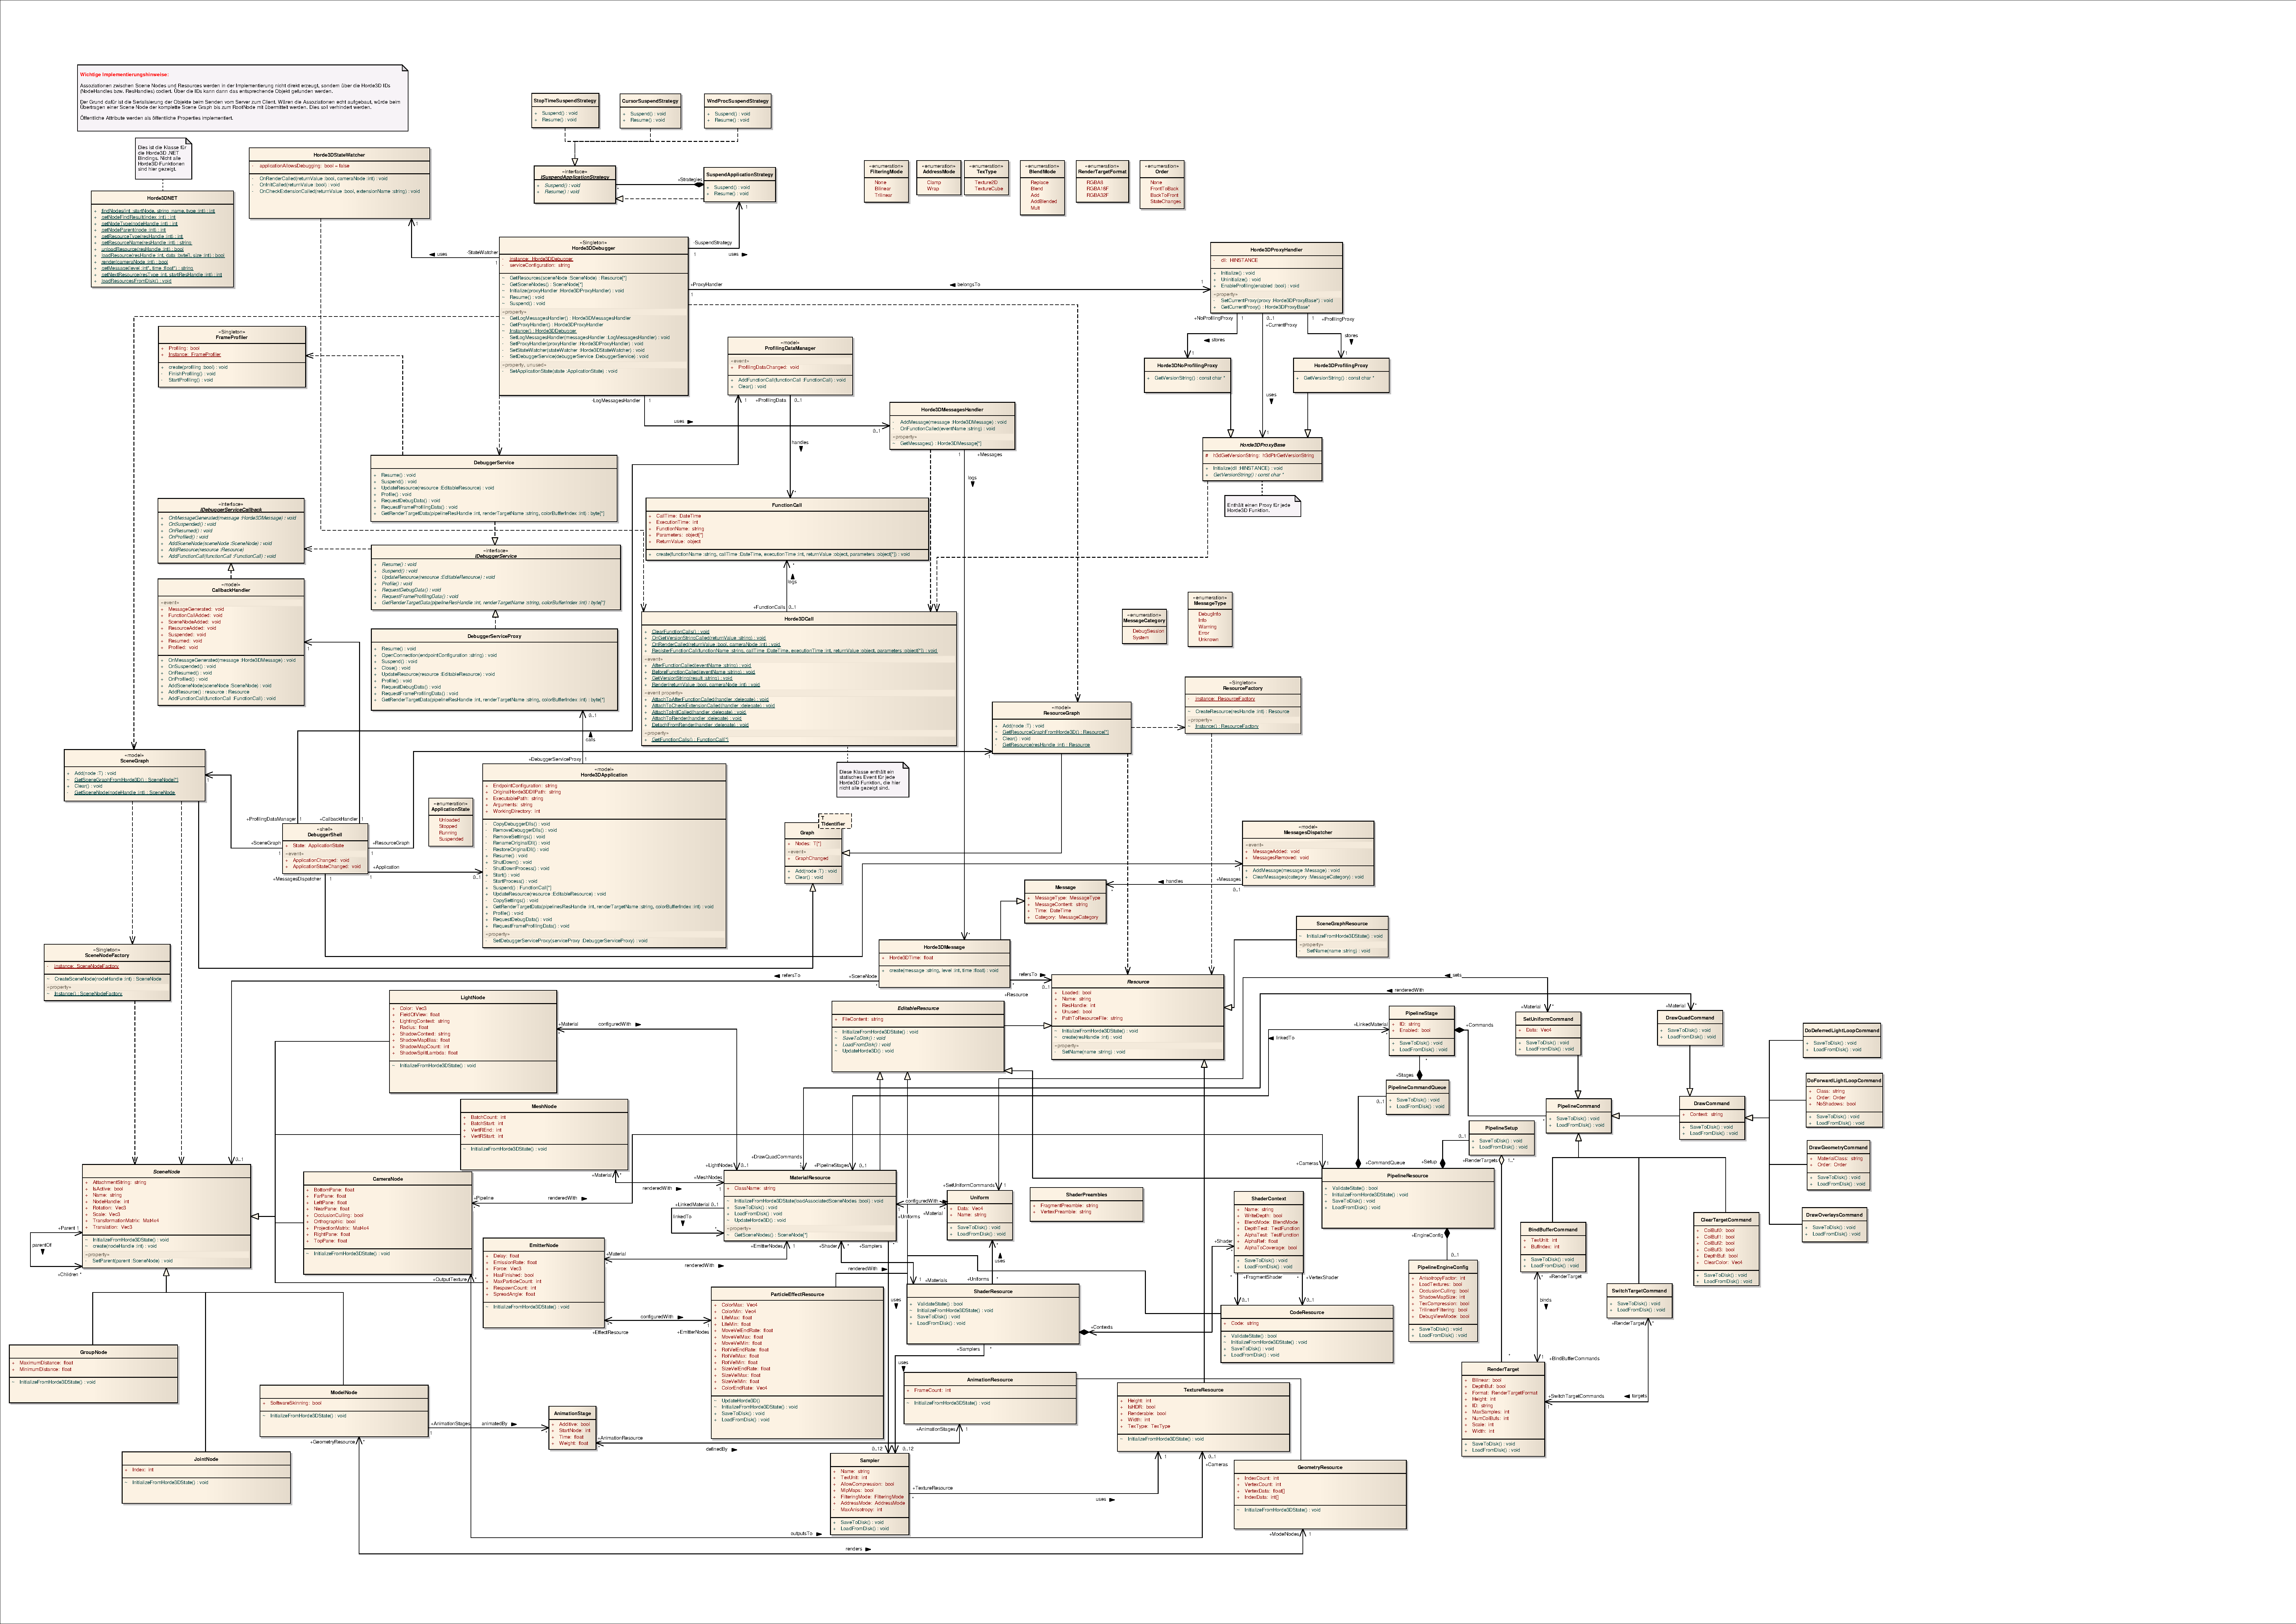
\includegraphics[trim = 250mm 725mm 760mm 40mm, clip, scale=0.7]{images/Designmodell.pdf}
\caption{Ausschnitt aus dem  Designklassen-Diagramm f�r die Anwendung des \emph{Strategy Patterns} zum Anhalten der Anwendung}\label{fig:suspendStrategyDesign}
\end{figure}

\begin{figure}[htp]
\centering
%trim=l b r t  	This option will crop the imported image by l from the left, b from the bottom, r from the right, and t  from the top. Where l, b, r and t are lengths. 
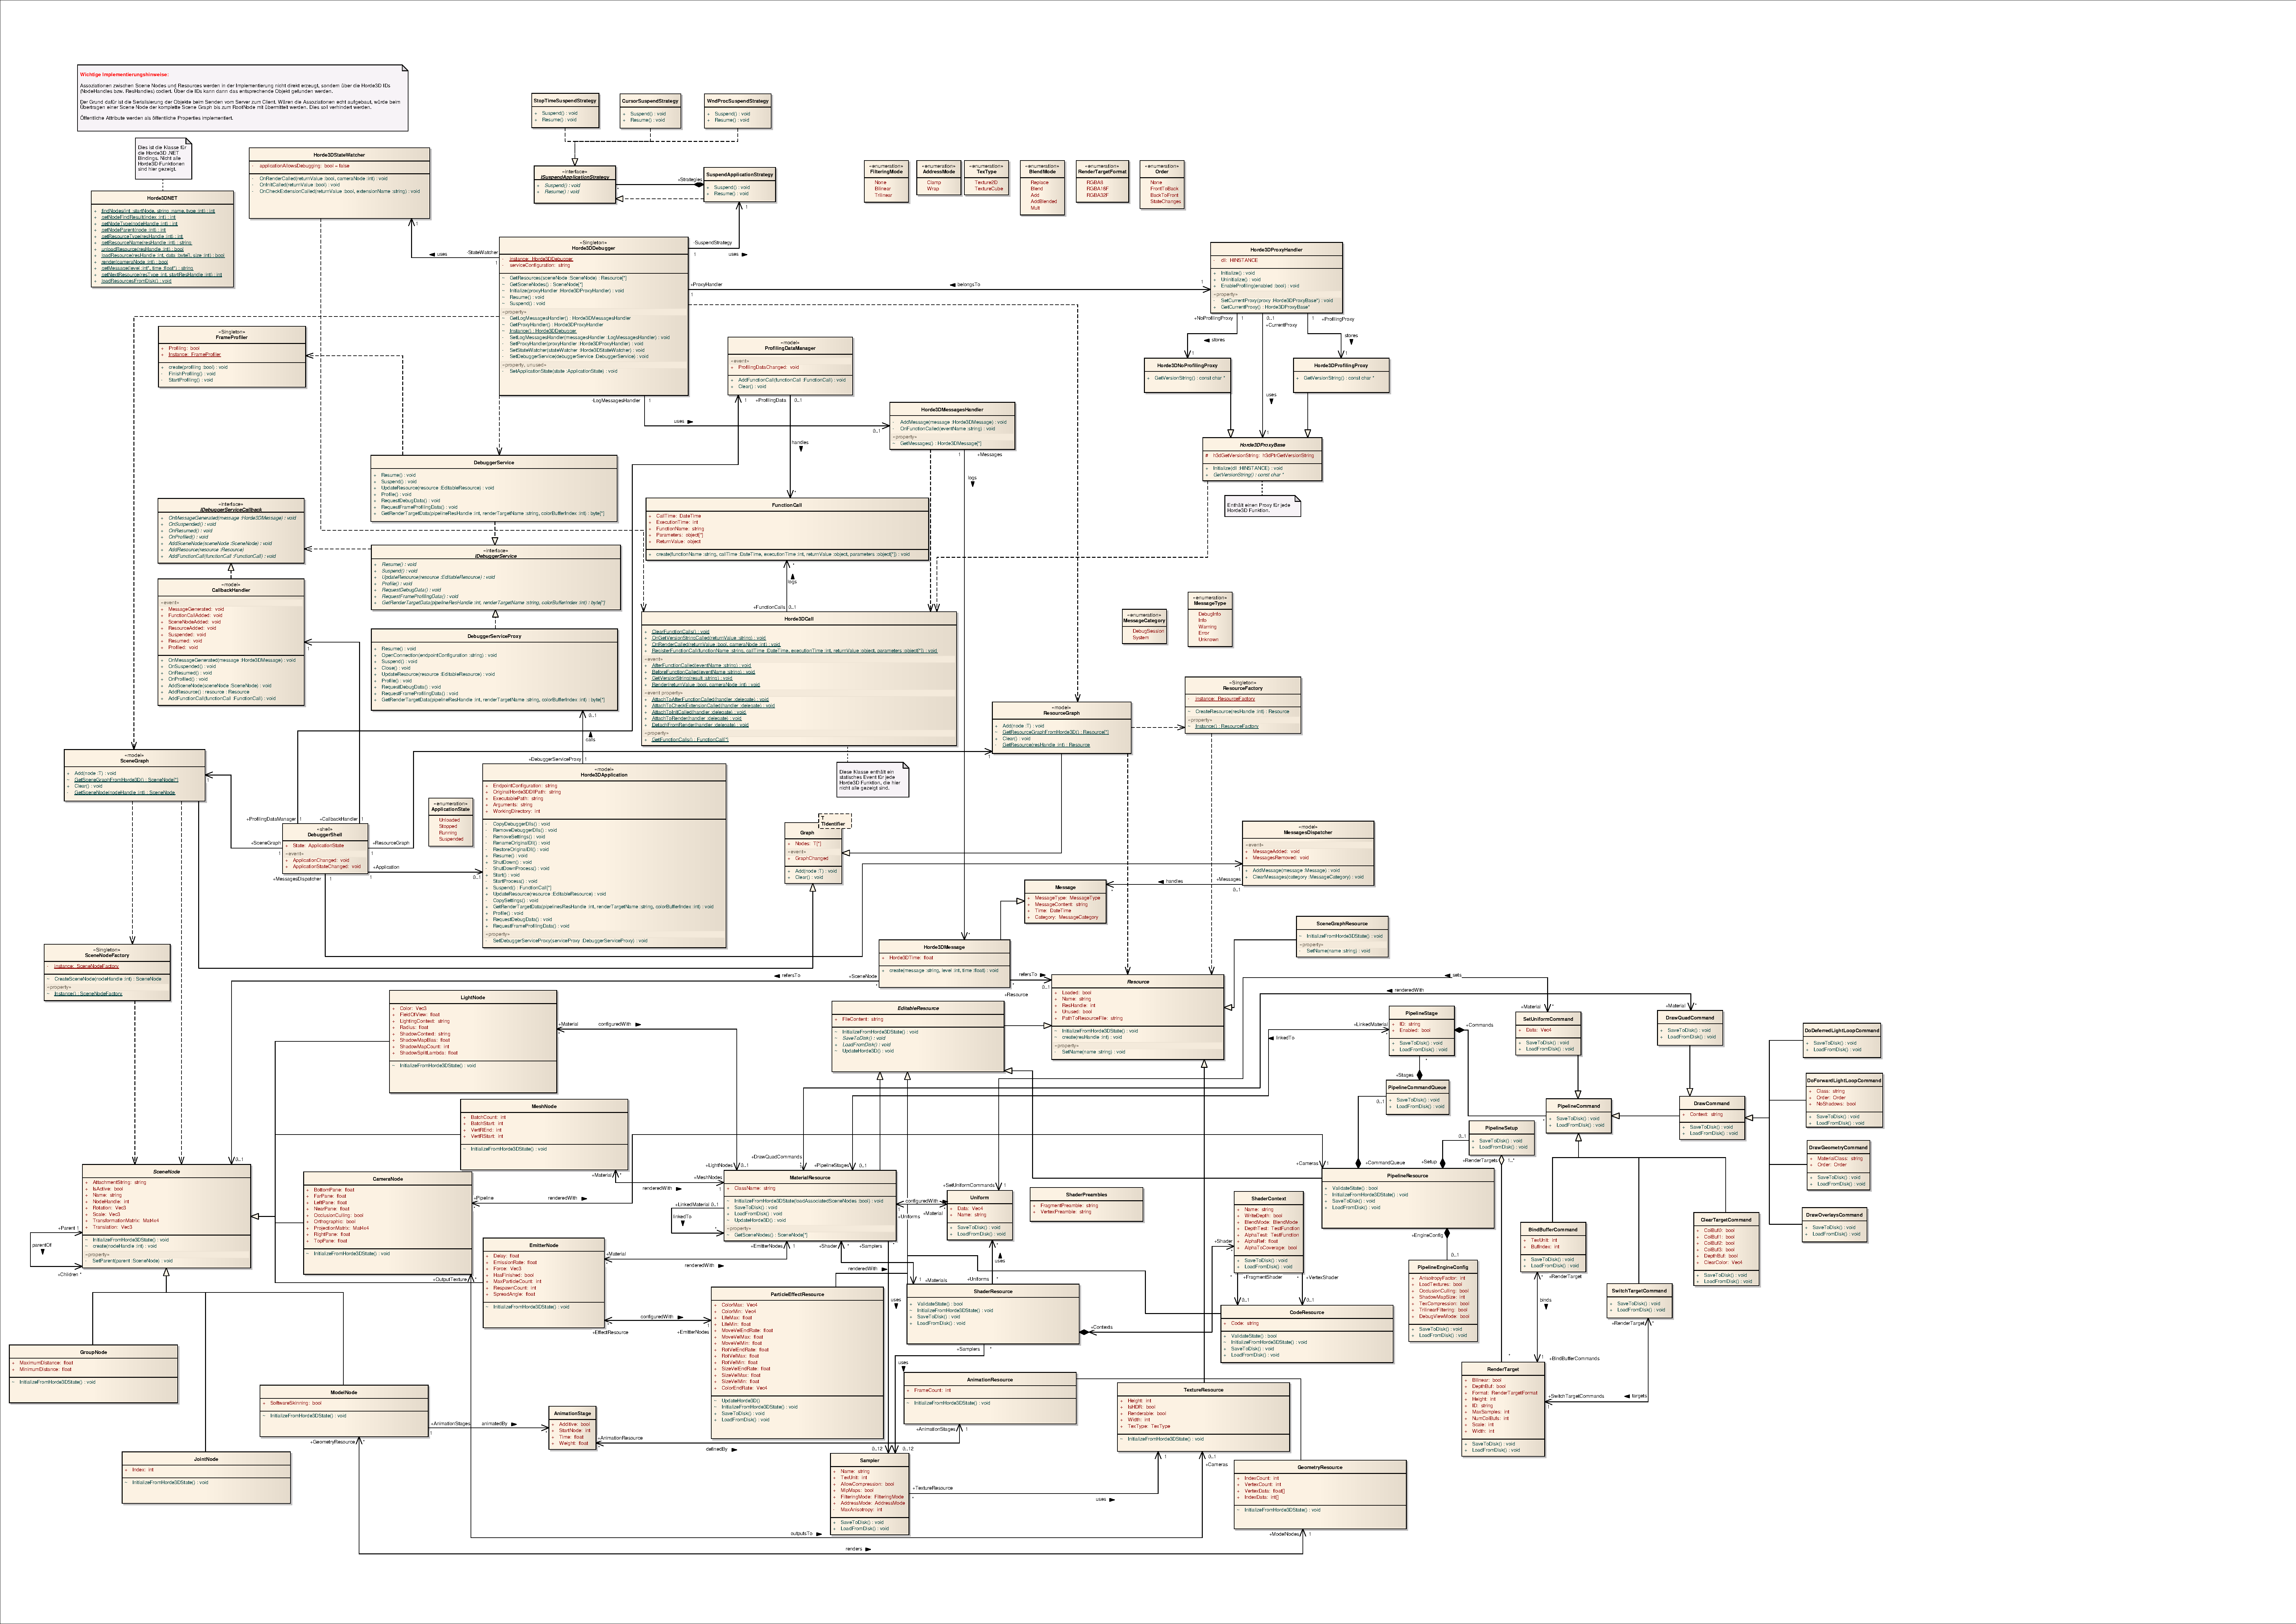
\includegraphics[trim = 585mm 570mm 450mm 125mm, clip, scale=0.7]{images/Designmodell.pdf}
\caption{Ausschnitt aus dem  Designklassen-Diagramm f�r die \Horde-\emph{Proxies}}\label{fig:proxyDesign}
\end{figure}

\begin{figure}[htp]
\centering
%trim=l b r t  	This option will crop the imported image by l from the left, b from the bottom, r from the right, and t  from the top. Where l, b, r and t are lengths. 
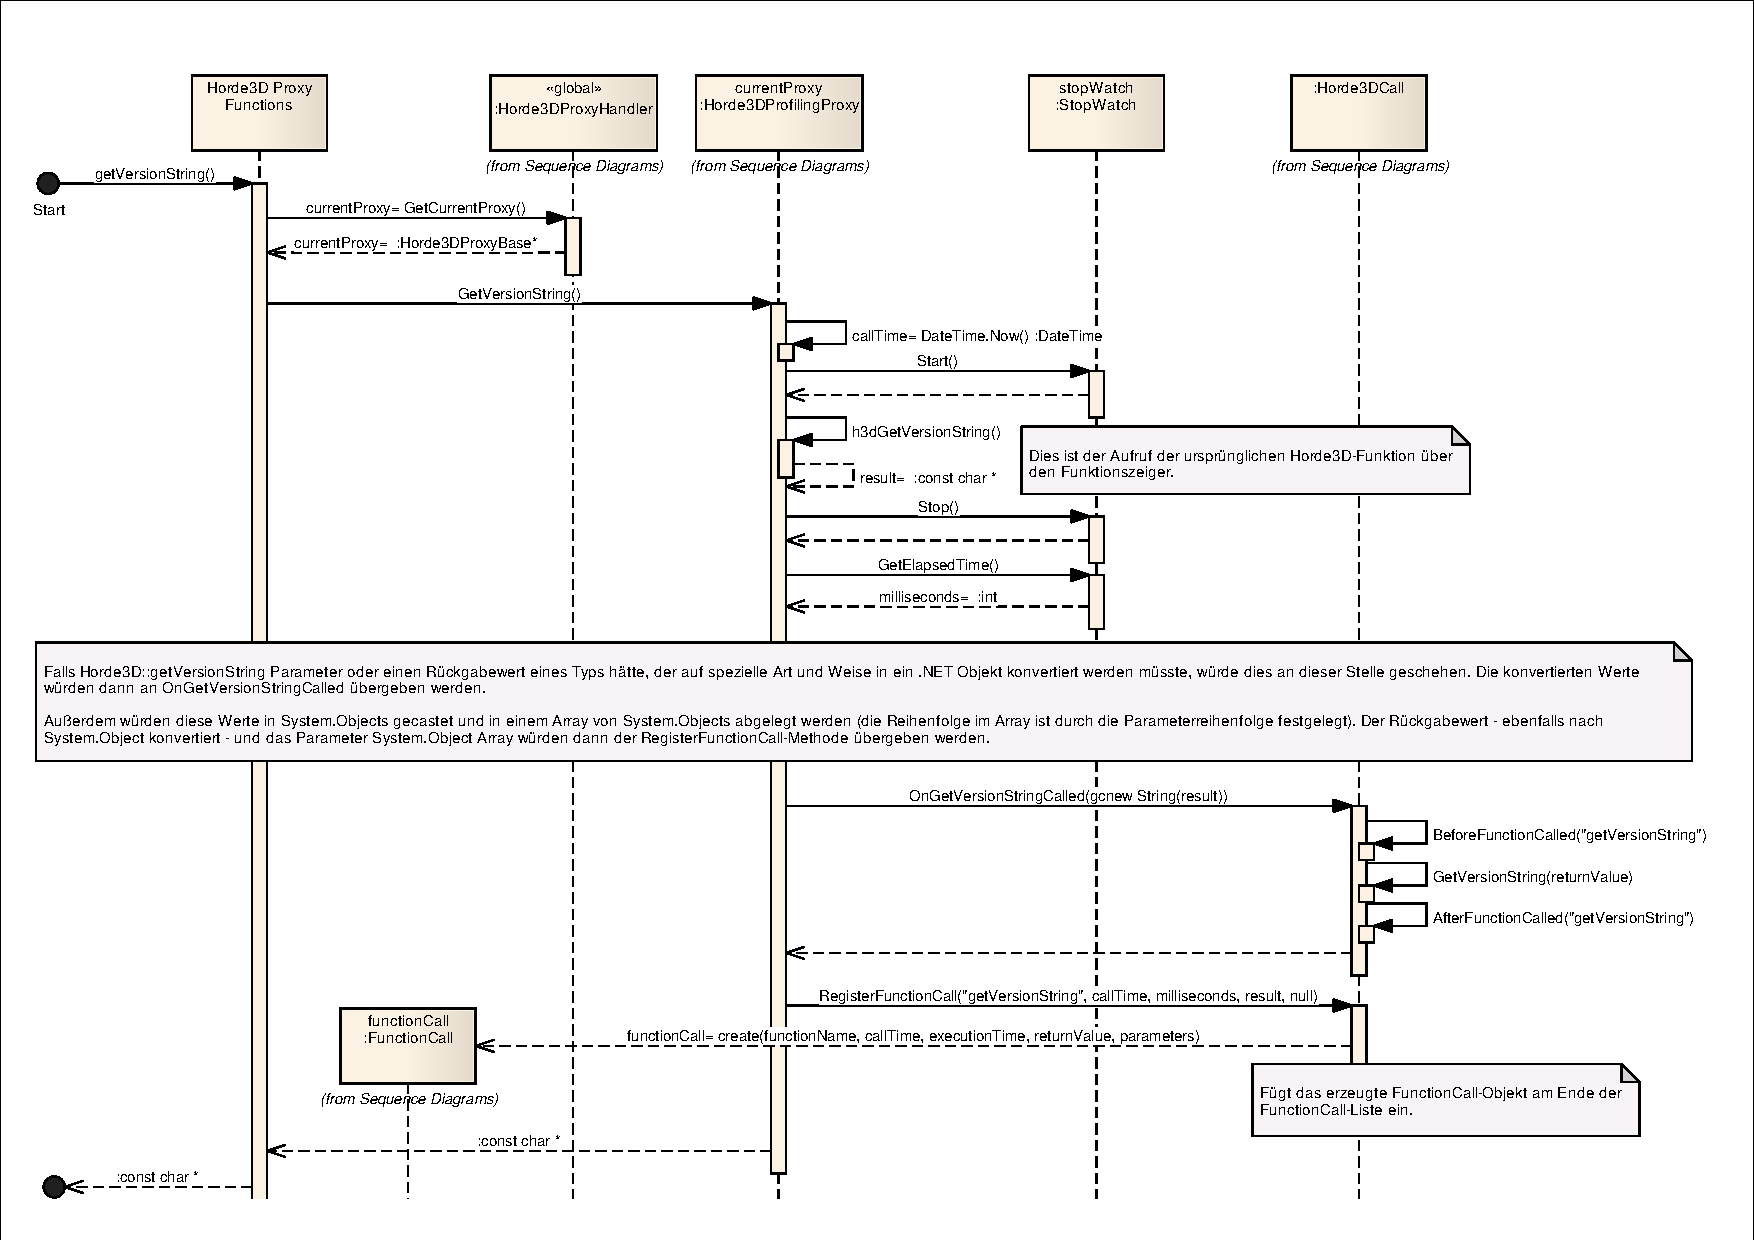
\includegraphics[trim = 5mm 1mm 1mm 5mm, clip, angle = 90, scale=0.7]{images/ProfilingProxySeq.pdf}
\caption{Sequenzdiagramm f�r den Aufruf von \texttt{Horde3D::getVersionString} bei aktiviertem Profiling}\label{fig:proxySeq}
\end{figure}

\begin{figure}[htp]
\centering
%trim=l b r t  	This option will crop the imported image by l from the left, b from the bottom, r from the right, and t  from the top. Where l, b, r and t are lengths. 
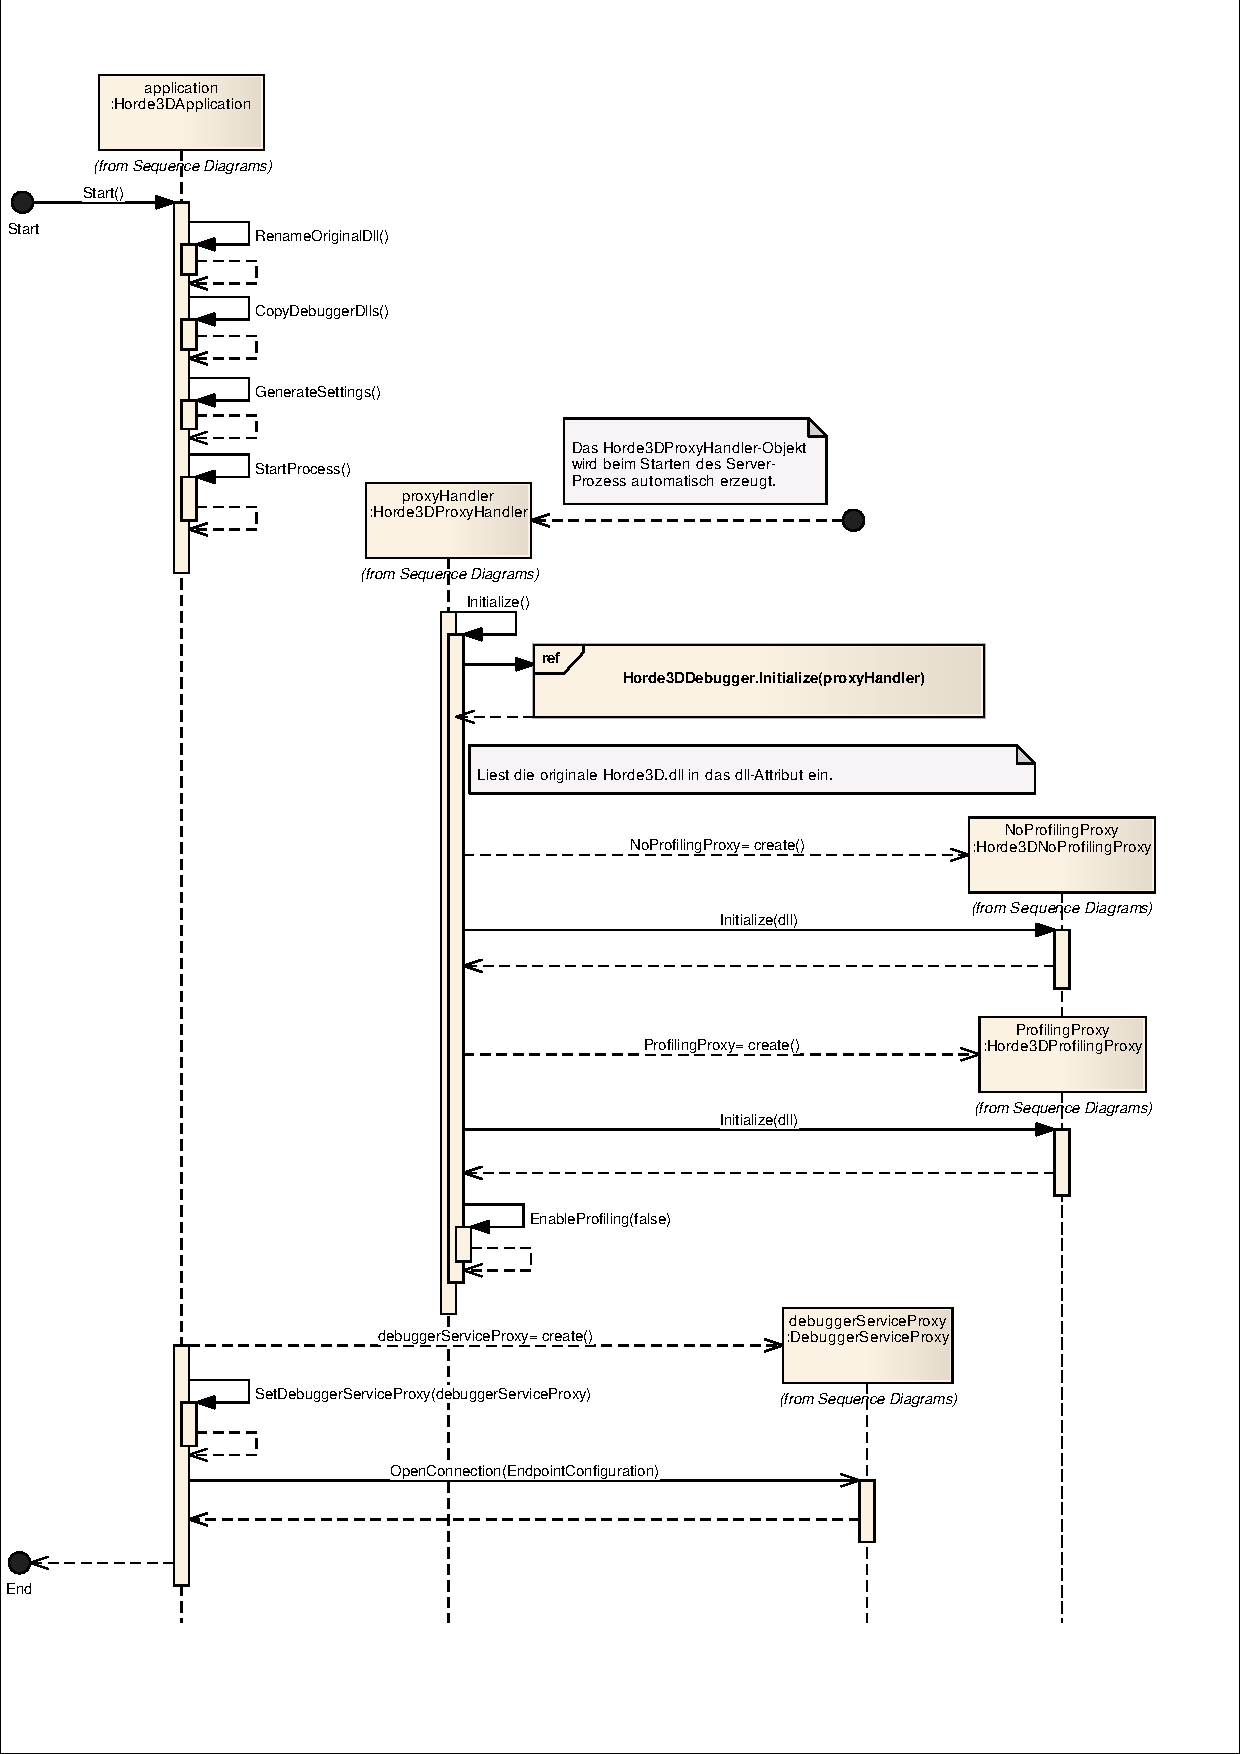
\includegraphics[trim = 1mm 20mm 10mm 5mm, clip, scale=0.7]{images/Horde3DApplication_Start.pdf}
\caption{Sequenzdiagramm f�r \texttt{Horde3DApplication.Start}}\label{fig:startSeq}
\end{figure}

\begin{figure}[htp]
\centering
%trim=l b r t  	This option will crop the imported image by l from the left, b from the bottom, r from the right, and t  from the top. Where l, b, r and t are lengths. 
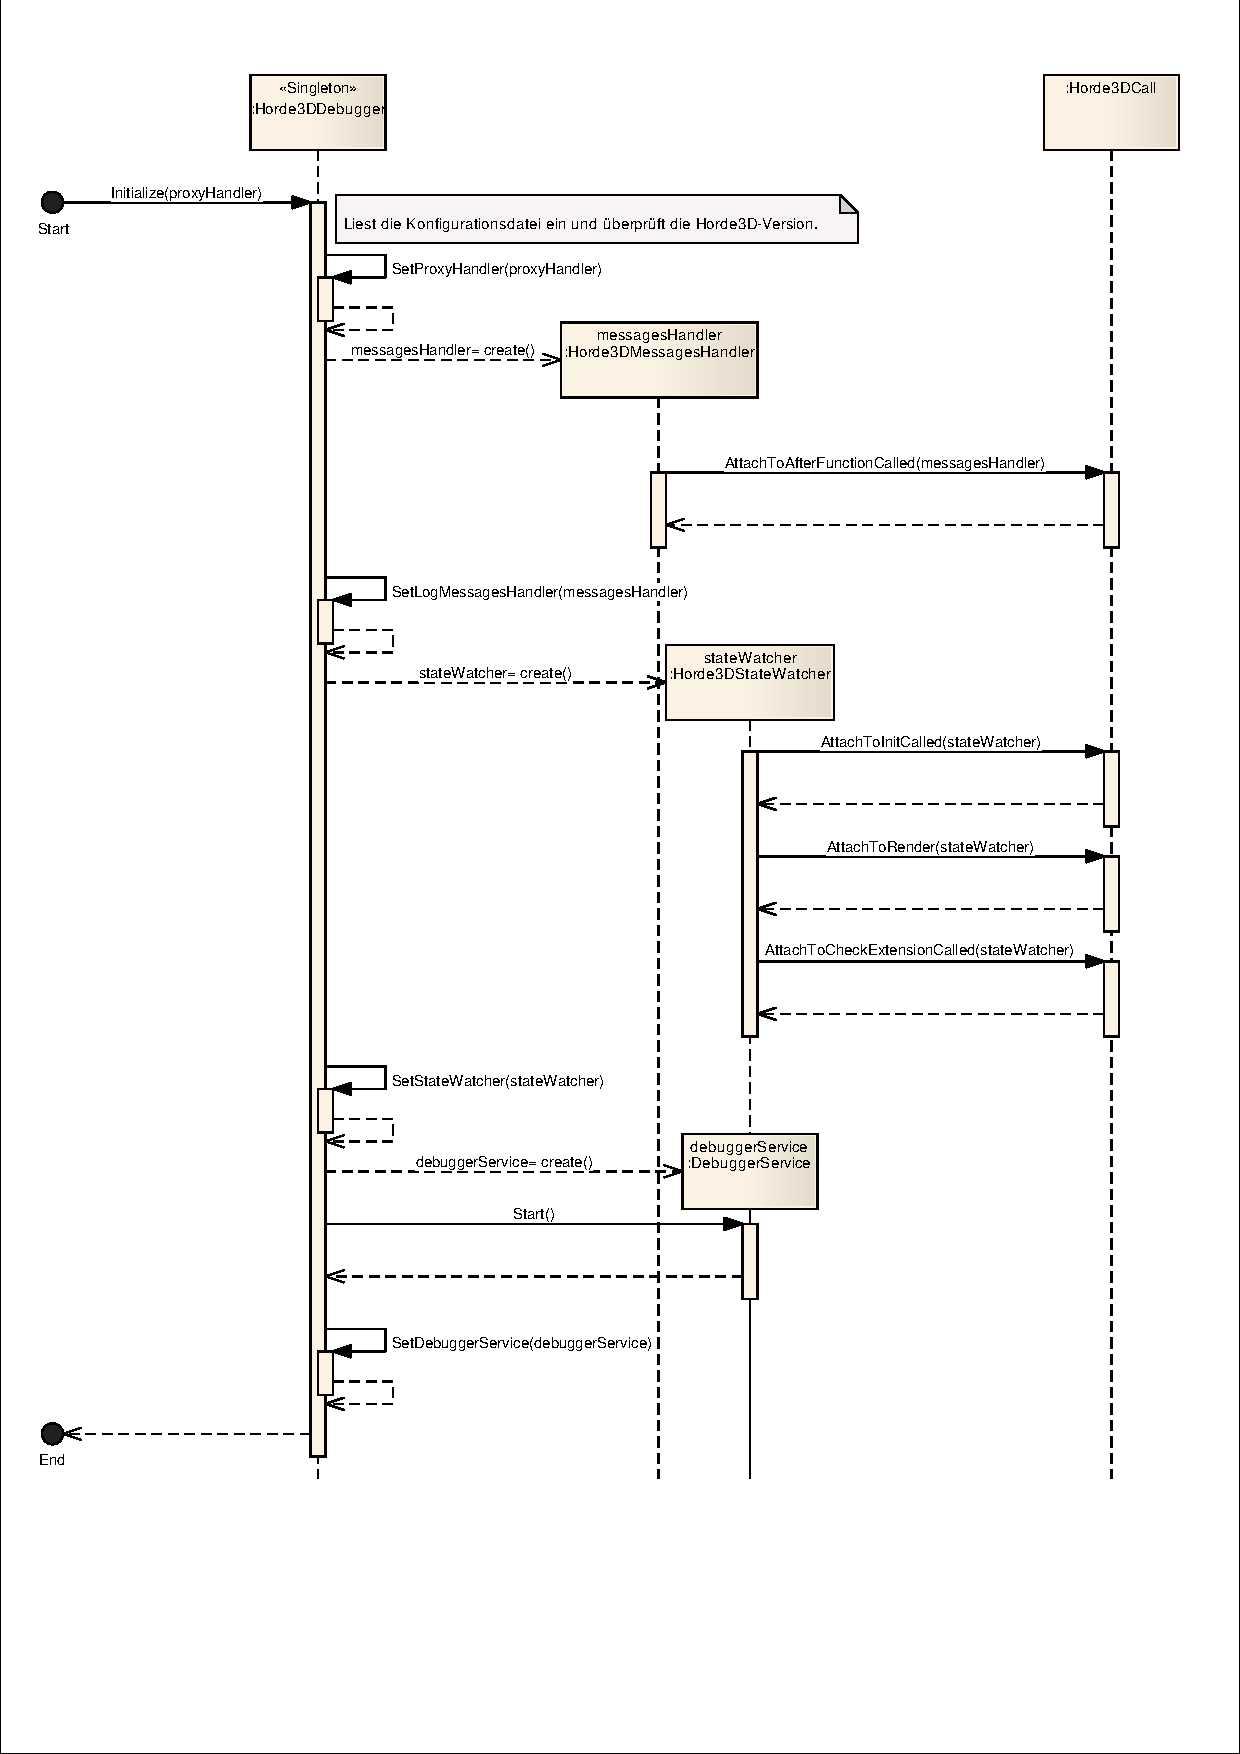
\includegraphics[trim = 5mm 45mm 5mm 5mm, clip, scale=0.7]{images/Horde3DDebugger_Initialize.pdf}
\caption{Sequenzdiagramm f�r \texttt{Horde3DDebugger.Initialize}}\label{fig:DebuggerInitSeq}
\end{figure}

\begin{figure}[htp]
\centering
%trim=l b r t  	This option will crop the imported image by l from the left, b from the bottom, r from the right, and t  from the top. Where l, b, r and t are lengths. 
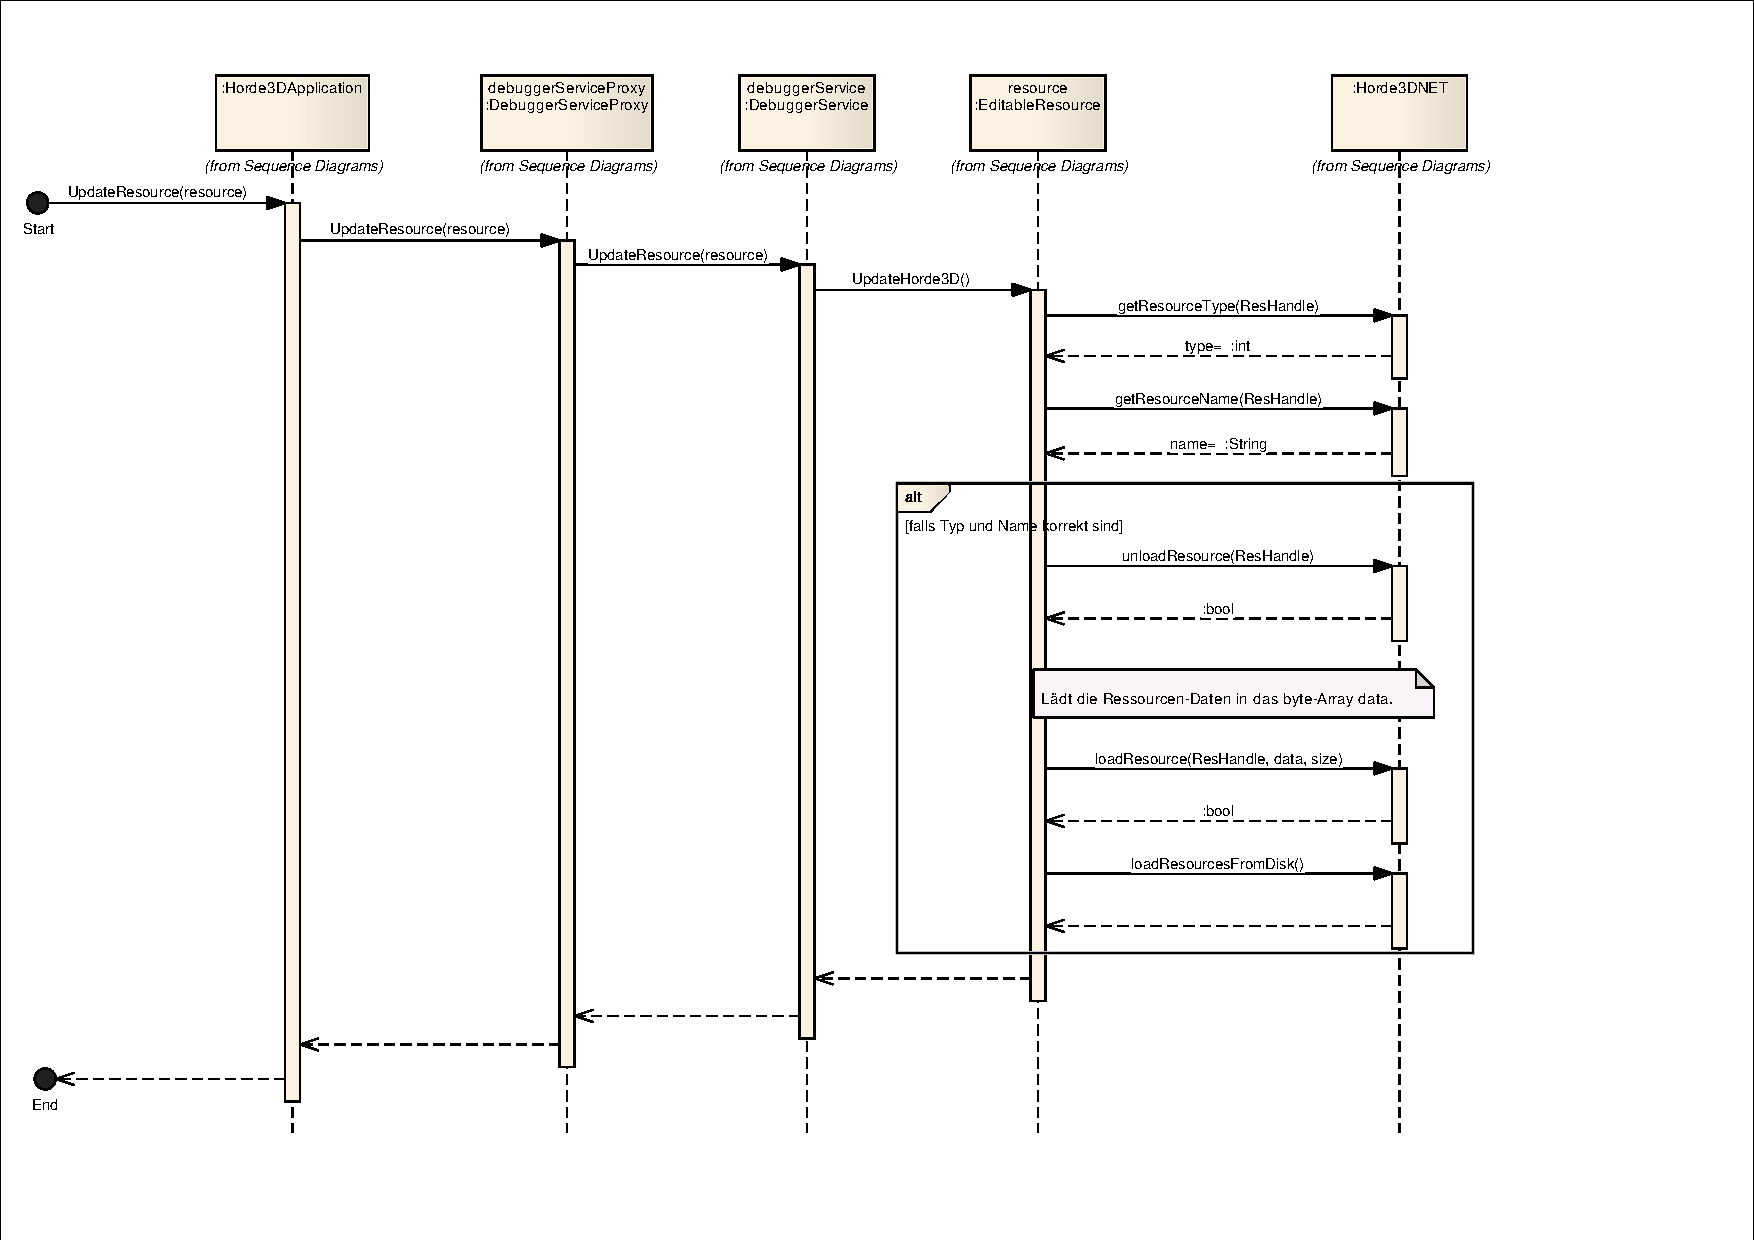
\includegraphics[trim = 1mm 15mm 5mm 5mm, clip, angle = 90, scale=0.7]{images/UpdateResource.pdf}
\caption{Sequenzdiagramm f�r \texttt{Horde3DApplication.UpdateResource}}\label{fig:UpdateResourceSeq}
\end{figure}

\begin{figure}[htp]
\centering
%trim=l b r t  	This option will crop the imported image by l from the left, b from the bottom, r from the right, and t  from the top. Where l, b, r and t are lengths. 
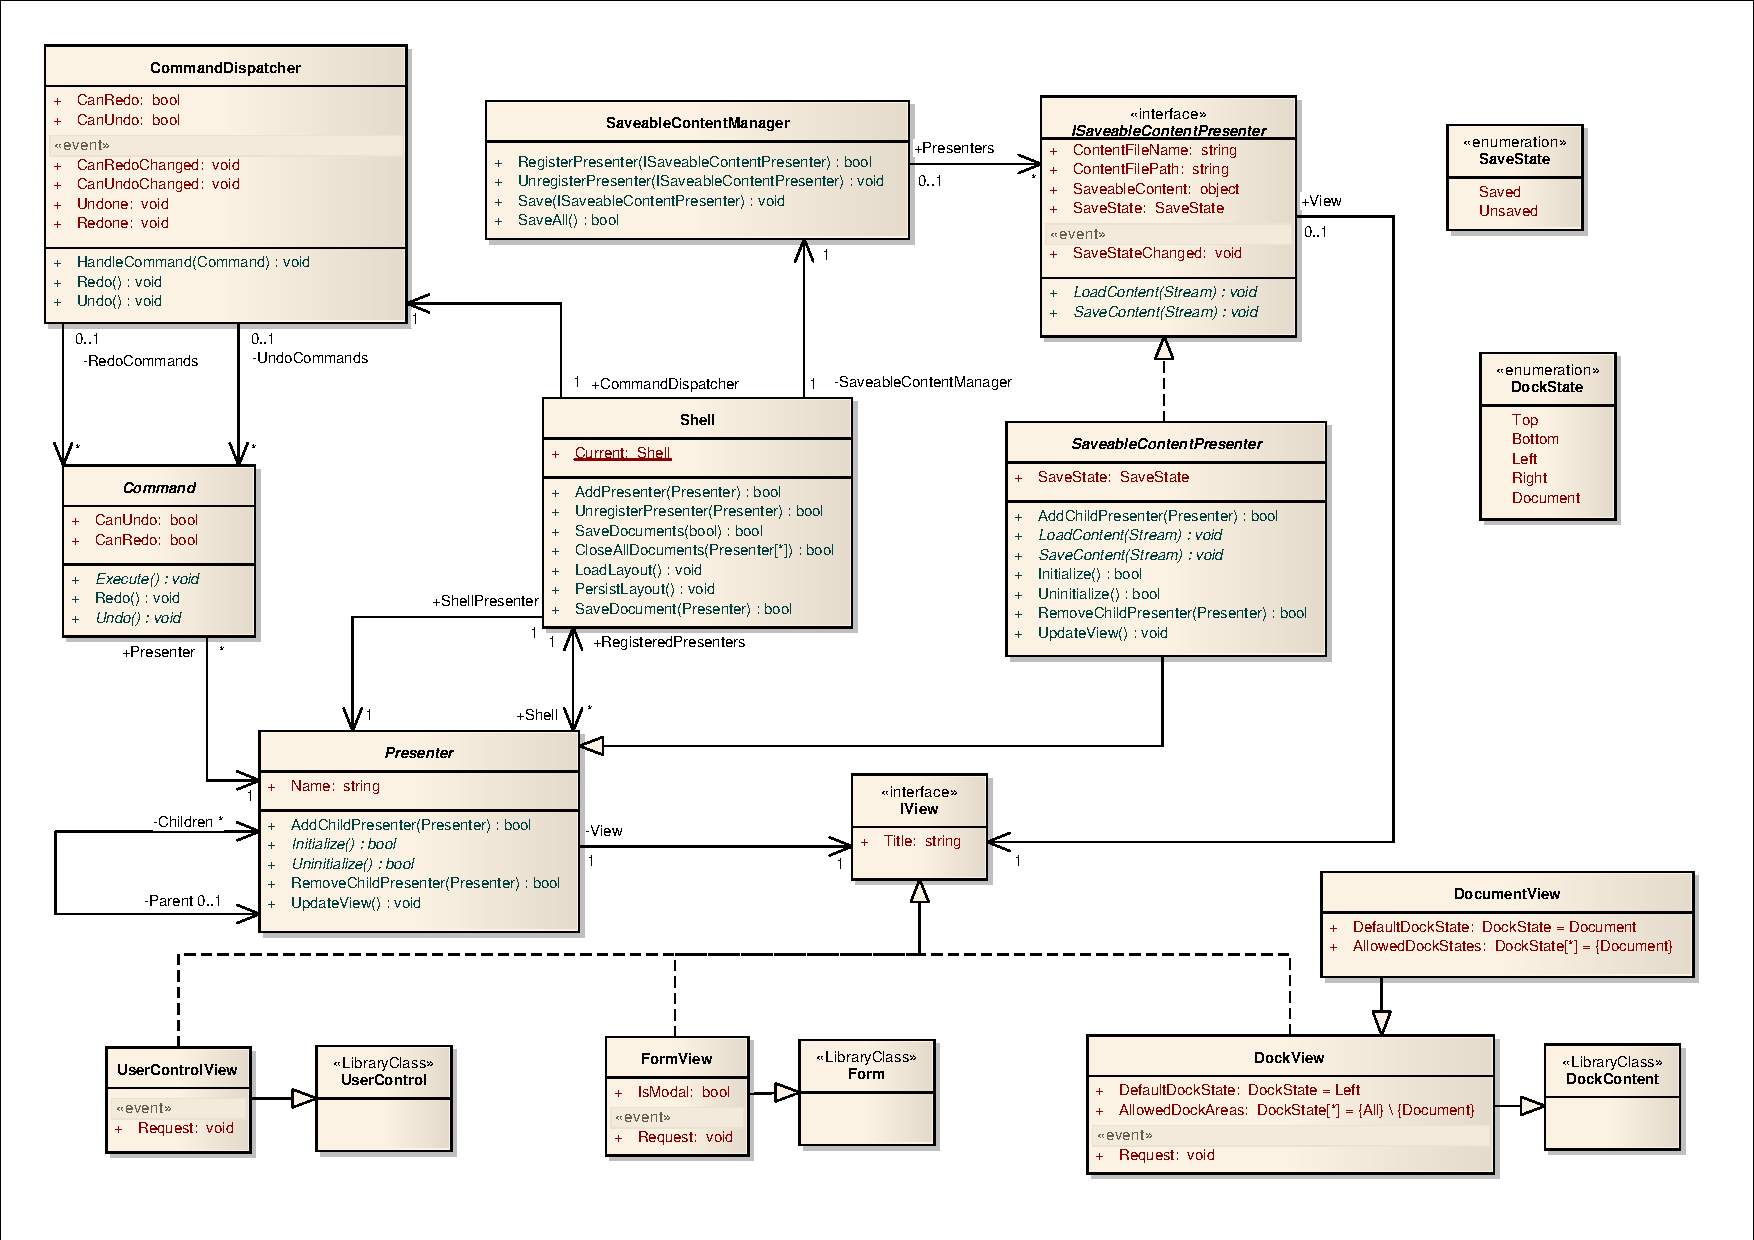
\includegraphics[trim = 5mm 5mm 5mm 5mm, clip, angle = 90, scale=0.7]{images/GuiClass.pdf}
\caption{Designklassen-Diagramm f�r das GUI-Framework}\label{fig:guiClass}
\end{figure}

\chapter{Artefakte der Implementierungs-Phase}

\begin{figure}[htp]
\centering
%trim=l b r t  	This option will crop the imported image by l from the left, b from the bottom, r from the right, and t  from the top. Where l, b, r and t are lengths. 
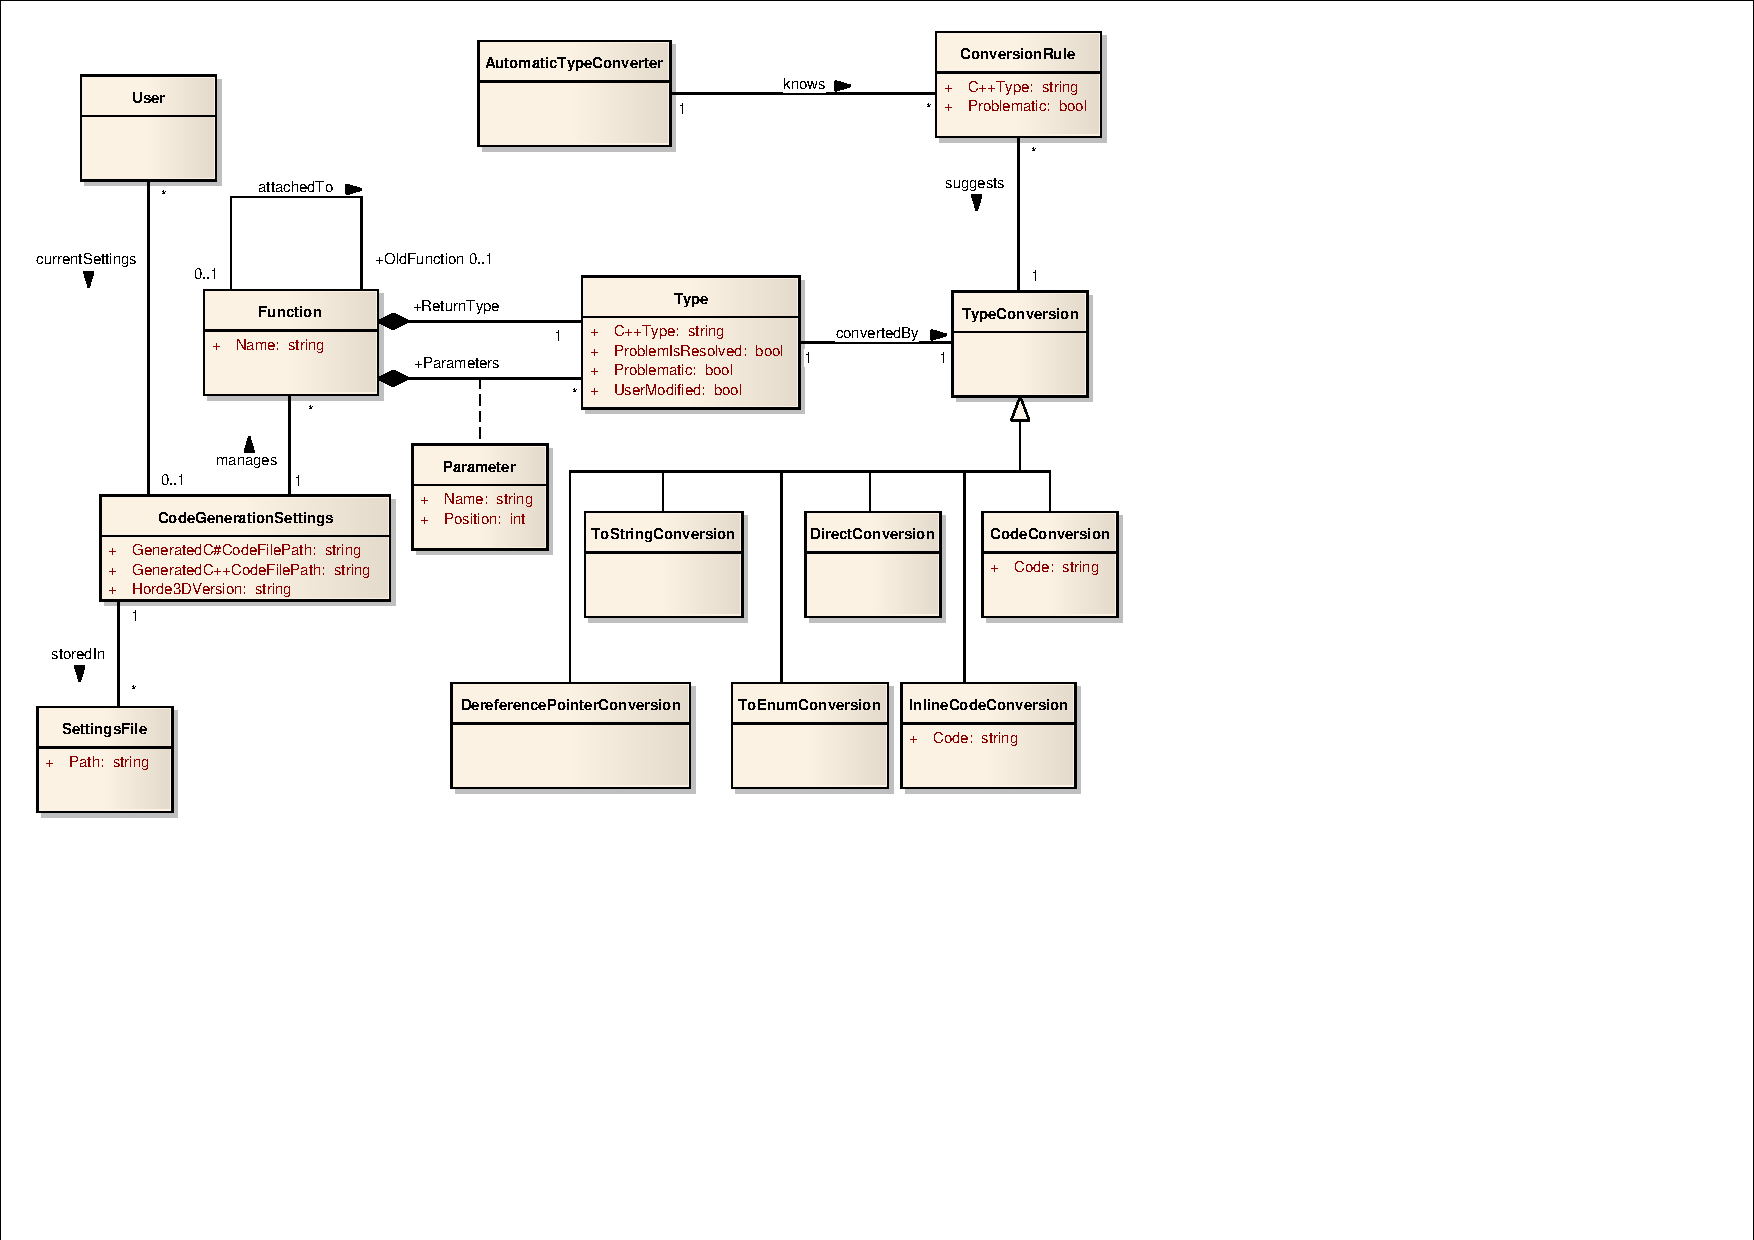
\includegraphics[trim = 5mm 70mm 85mm 5mm, clip, angle = 0, scale=0.7]{images/CodeGen_DomainModell.pdf}
\caption{Das Konzeptmodell des Code Generators}\label{fig:cgDomain}
\end{figure}

\begin{figure}[htp]
\centering
%trim=l b r t  	This option will crop the imported image by l from the left, b from the bottom, r from the right, and t  from the top. Where l, b, r and t are lengths. 
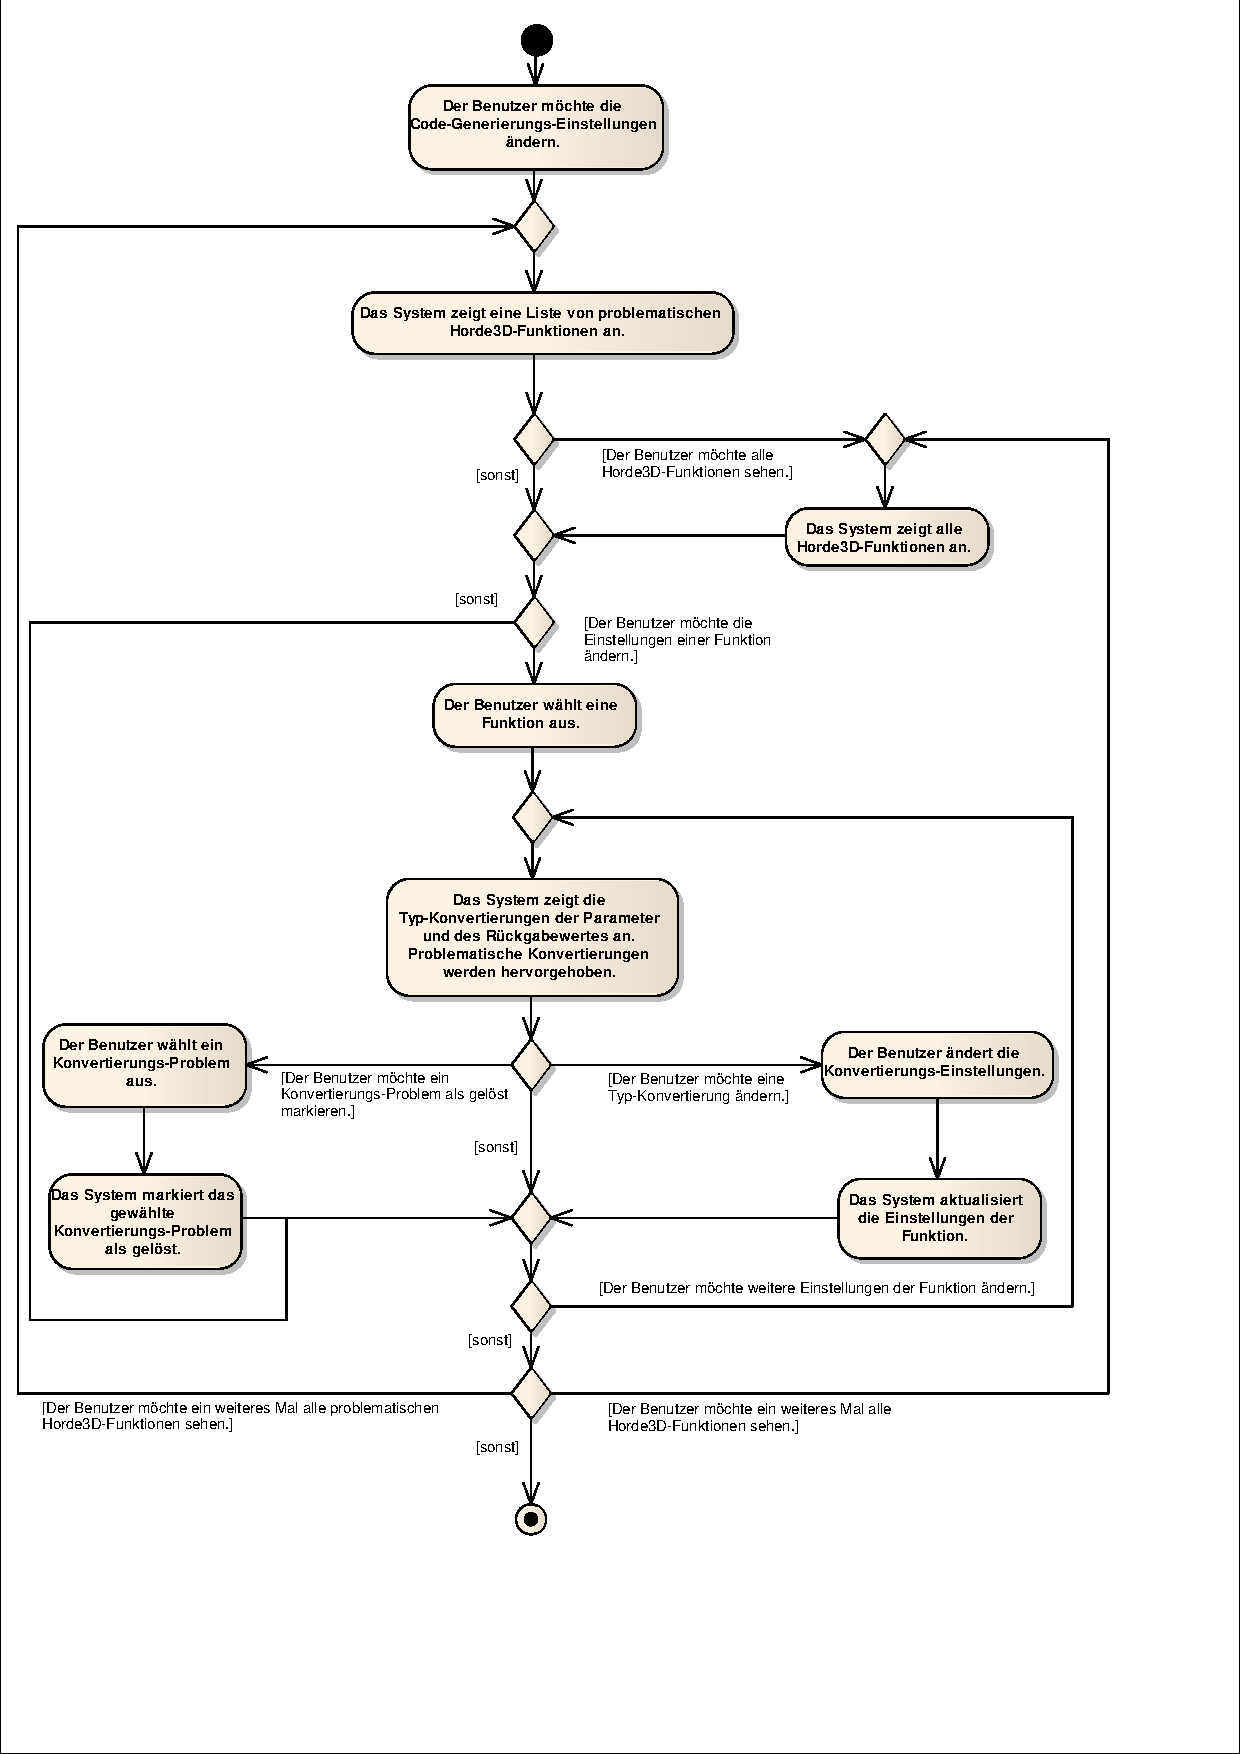
\includegraphics[trim = 1mm 30mm 20mm 1mm, clip, scale=0.7]{images/CodeGen_Change.pdf}
\caption{Aktivit�tsdiagramm f�r den Anwendungsfall "`�ndern der Einstellungen der Code-Generierung"'}\label{fig:cgChange}
\end{figure}

\begin{figure}[htp]
\centering
%trim=l b r t  	This option will crop the imported image by l from the left, b from the bottom, r from the right, and t  from the top. Where l, b, r and t are lengths. 
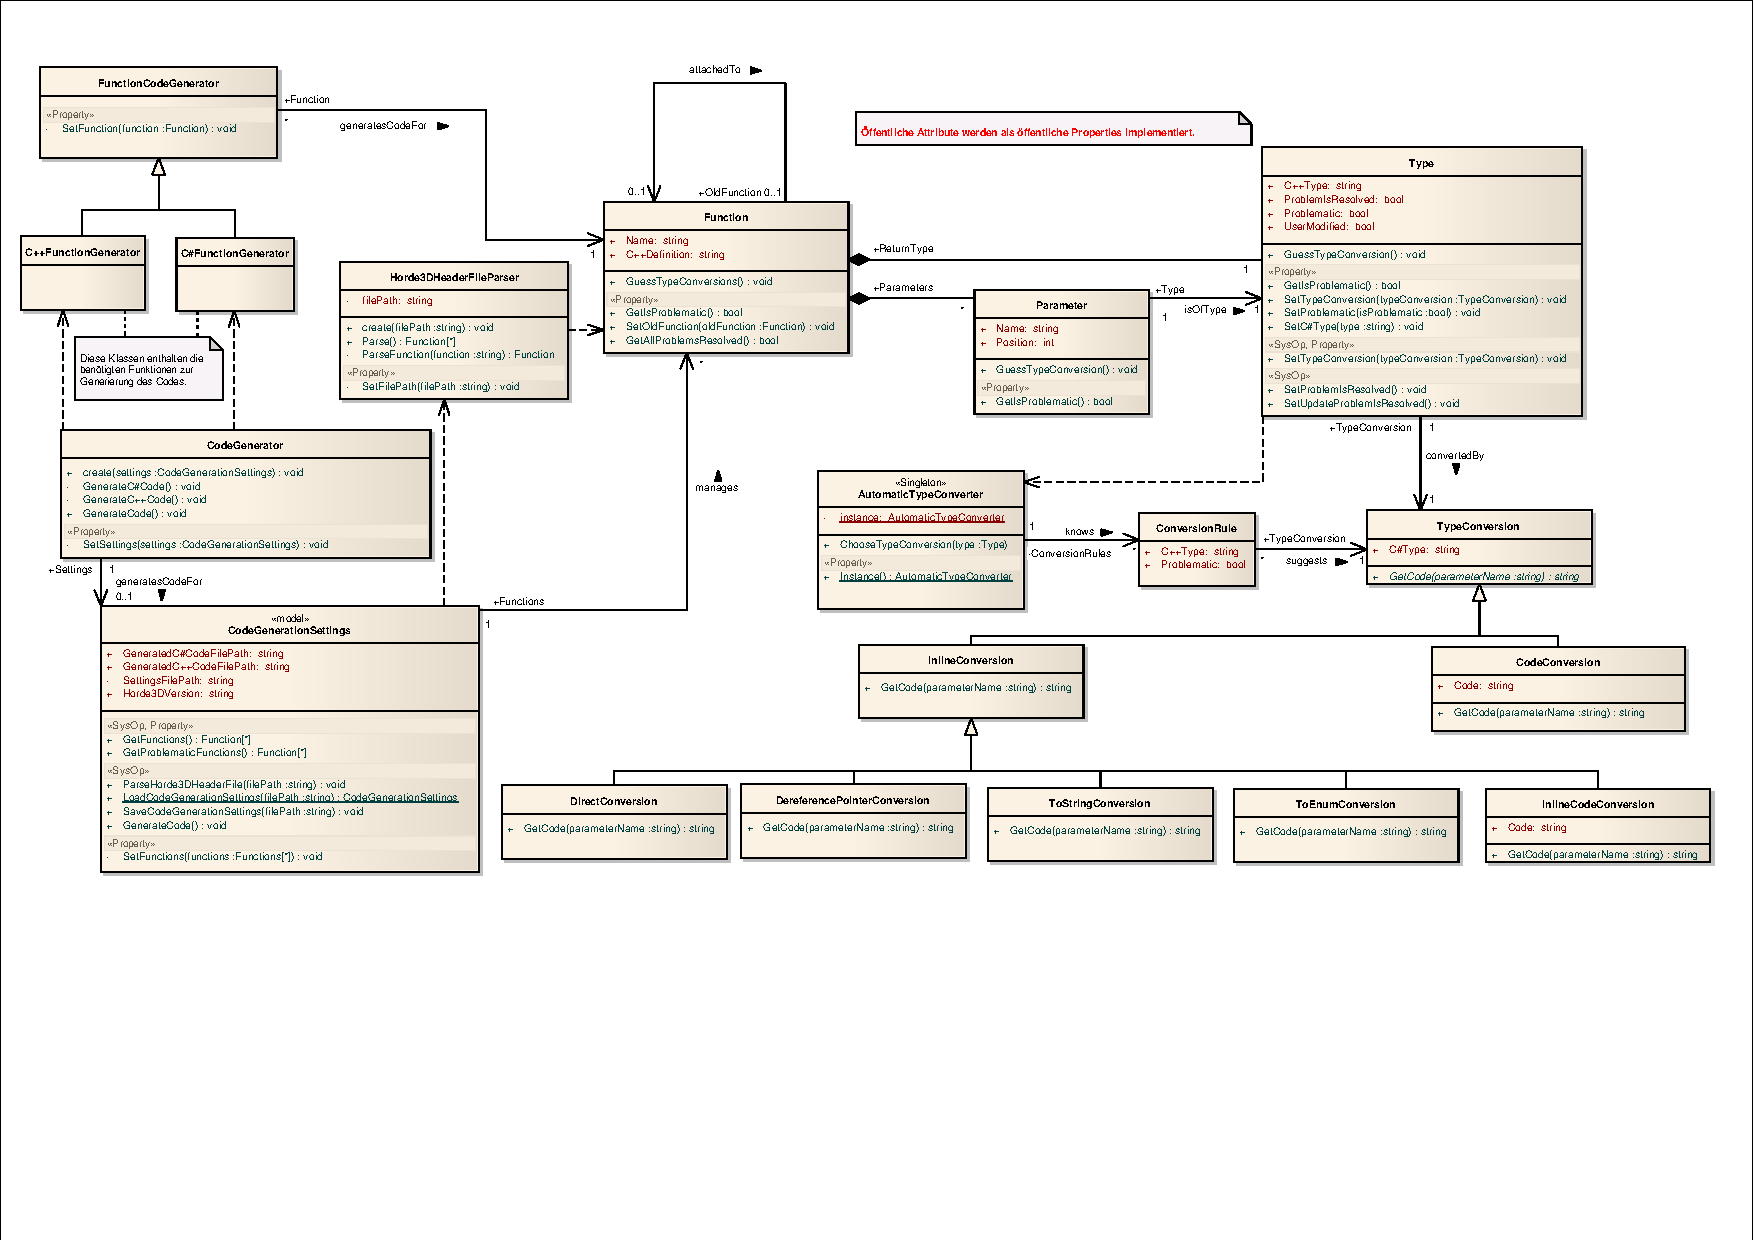
\includegraphics[trim = 1mm 30mm 1mm 1mm, angle = 90, clip, scale=0.7]{images/CodeGen_DesignModell.pdf}
\caption{Das Designmodell des Code Generators}\label{fig:cgDesign}
\end{figure}

\begin{figure}[htp]
\centering
%trim=l b r t  	This option will crop the imported image by l from the left, b from the bottom, r from the right, and t  from the top. Where l, b, r and t are lengths. 
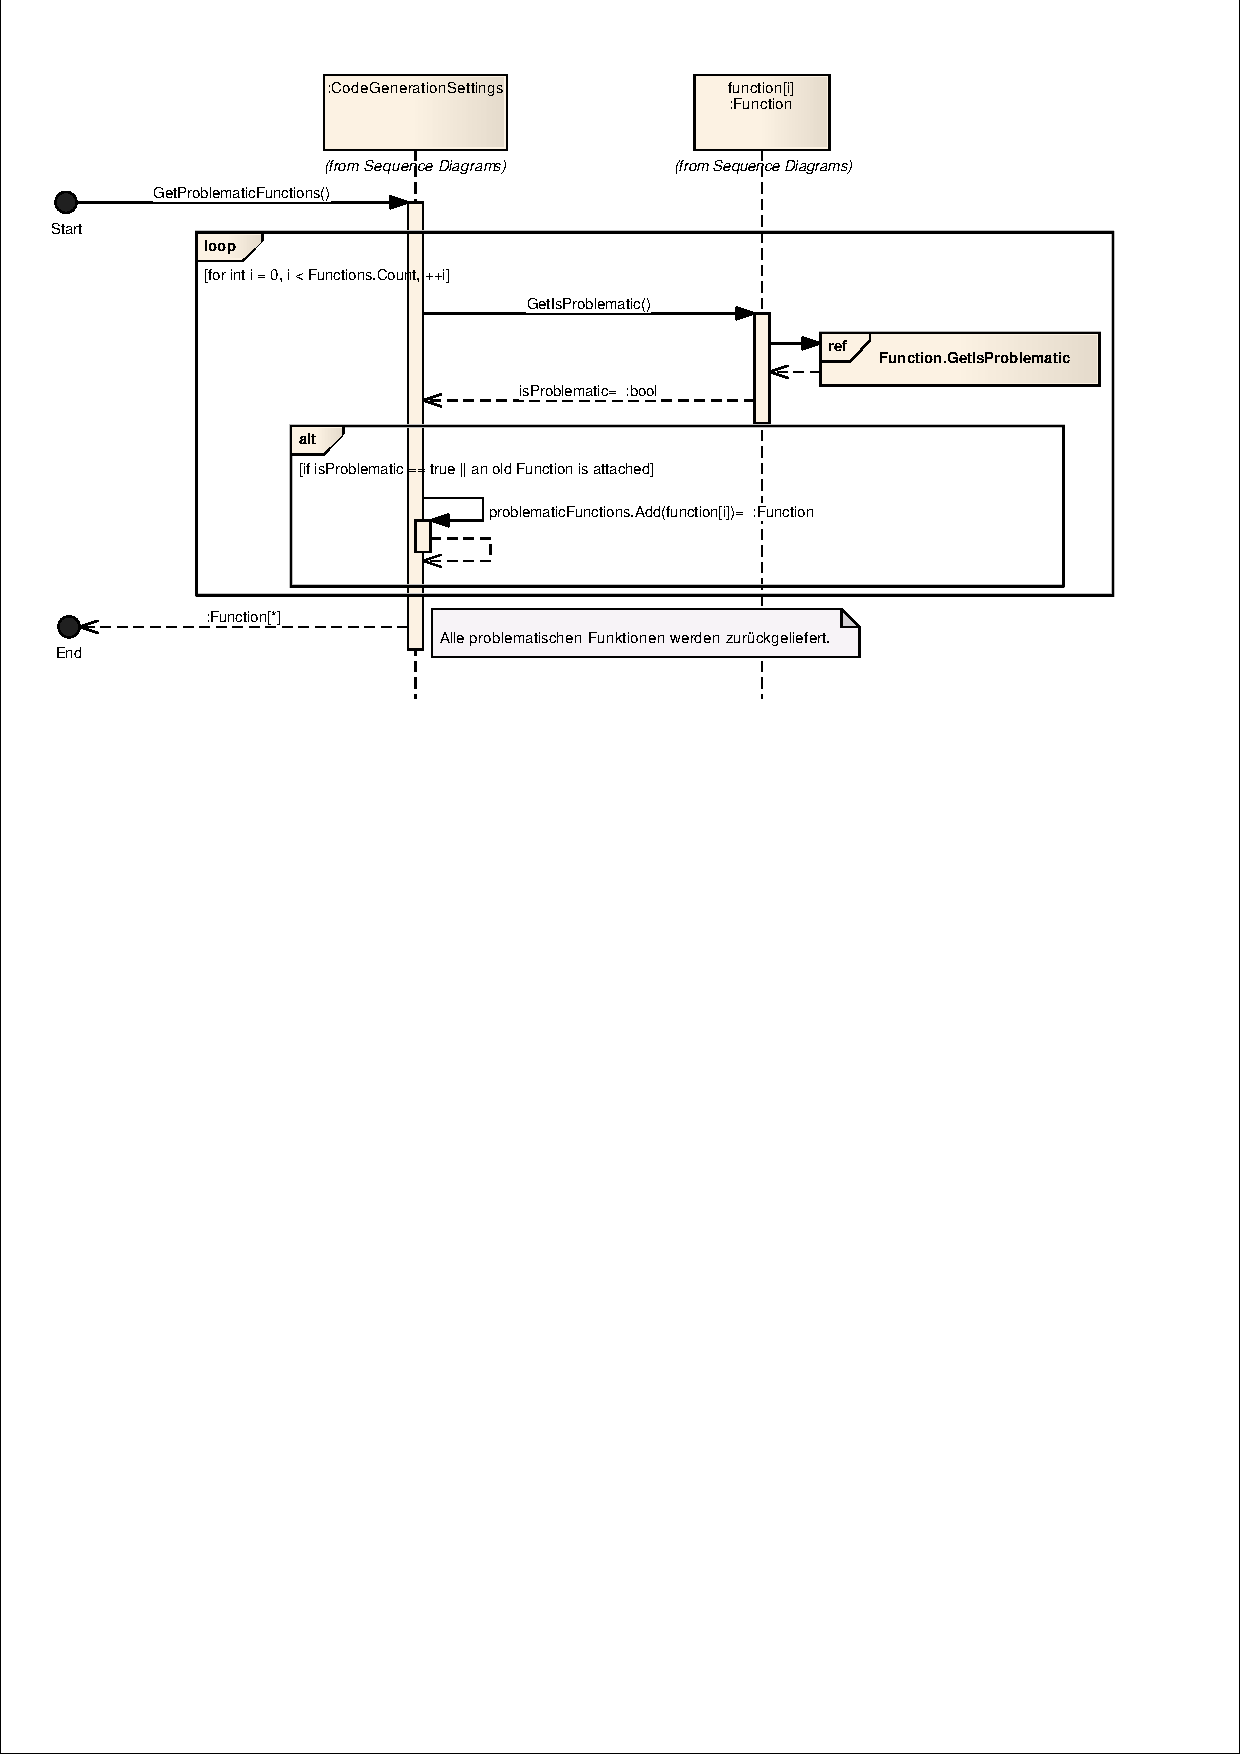
\includegraphics[trim = 1mm 180mm 1mm 1mm, clip, scale=0.7]{images/CodeGen_GetProblematicFunctions.pdf}
\caption{Sequenzdiagramm zum Auslesen aller problematischer Funktionen}\label{fig:cgGetPFunc}
\end{figure}

\begin{figure}[htp]
\centering
%trim=l b r t  	This option will crop the imported image by l from the left, b from the bottom, r from the right, and t  from the top. Where l, b, r and t are lengths. 
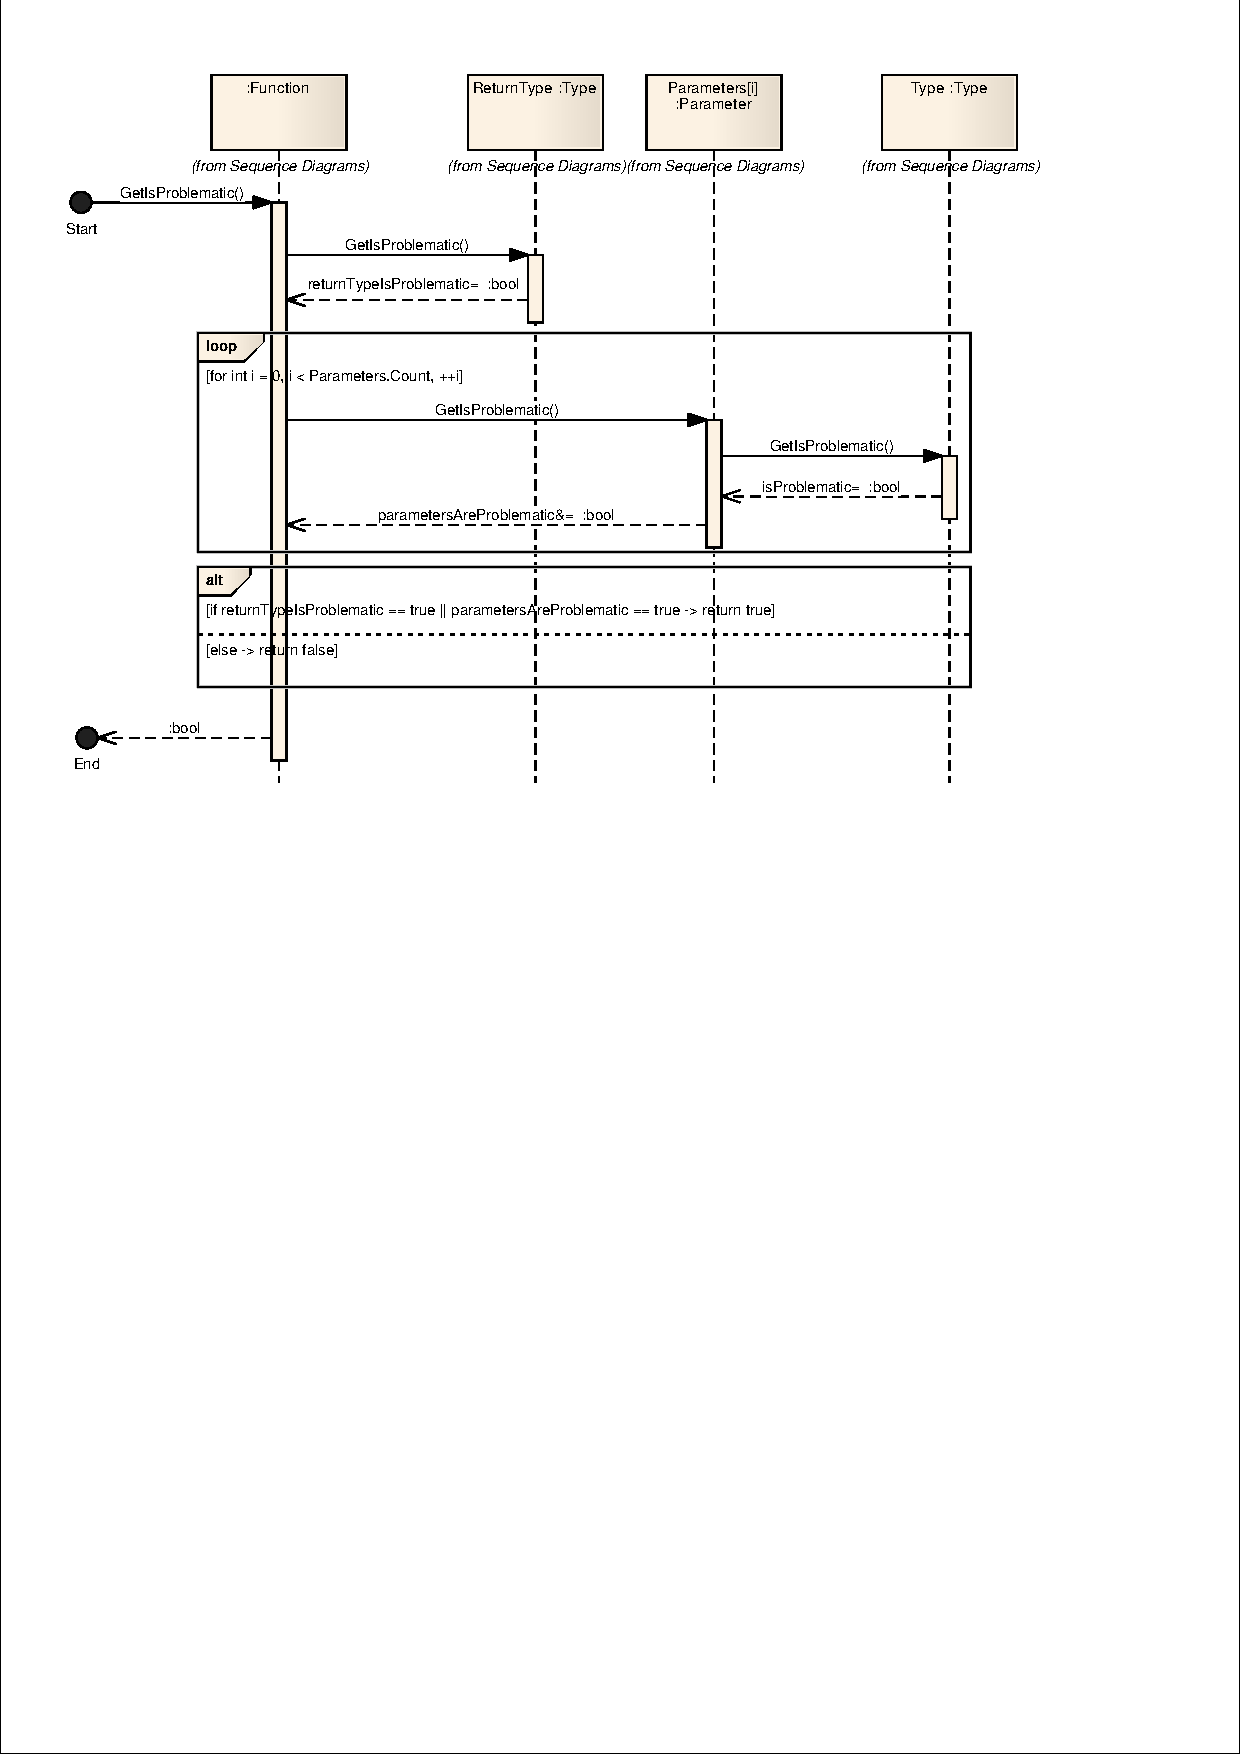
\includegraphics[trim = 1mm 165mm 20mm 1mm, clip, scale=0.7]{images/CodeGen_GetIsProblematic.pdf}
\caption{Sequenzdiagramm f�r das \emph{Property} \texttt{Function.IsProblematic}}\label{fig:cgIsProb}
\end{figure}

\begin{figure}[htp]
\centering
%trim=l b r t  	This option will crop the imported image by l from the left, b from the bottom, r from the right, and t  from the top. Where l, b, r and t are lengths. 
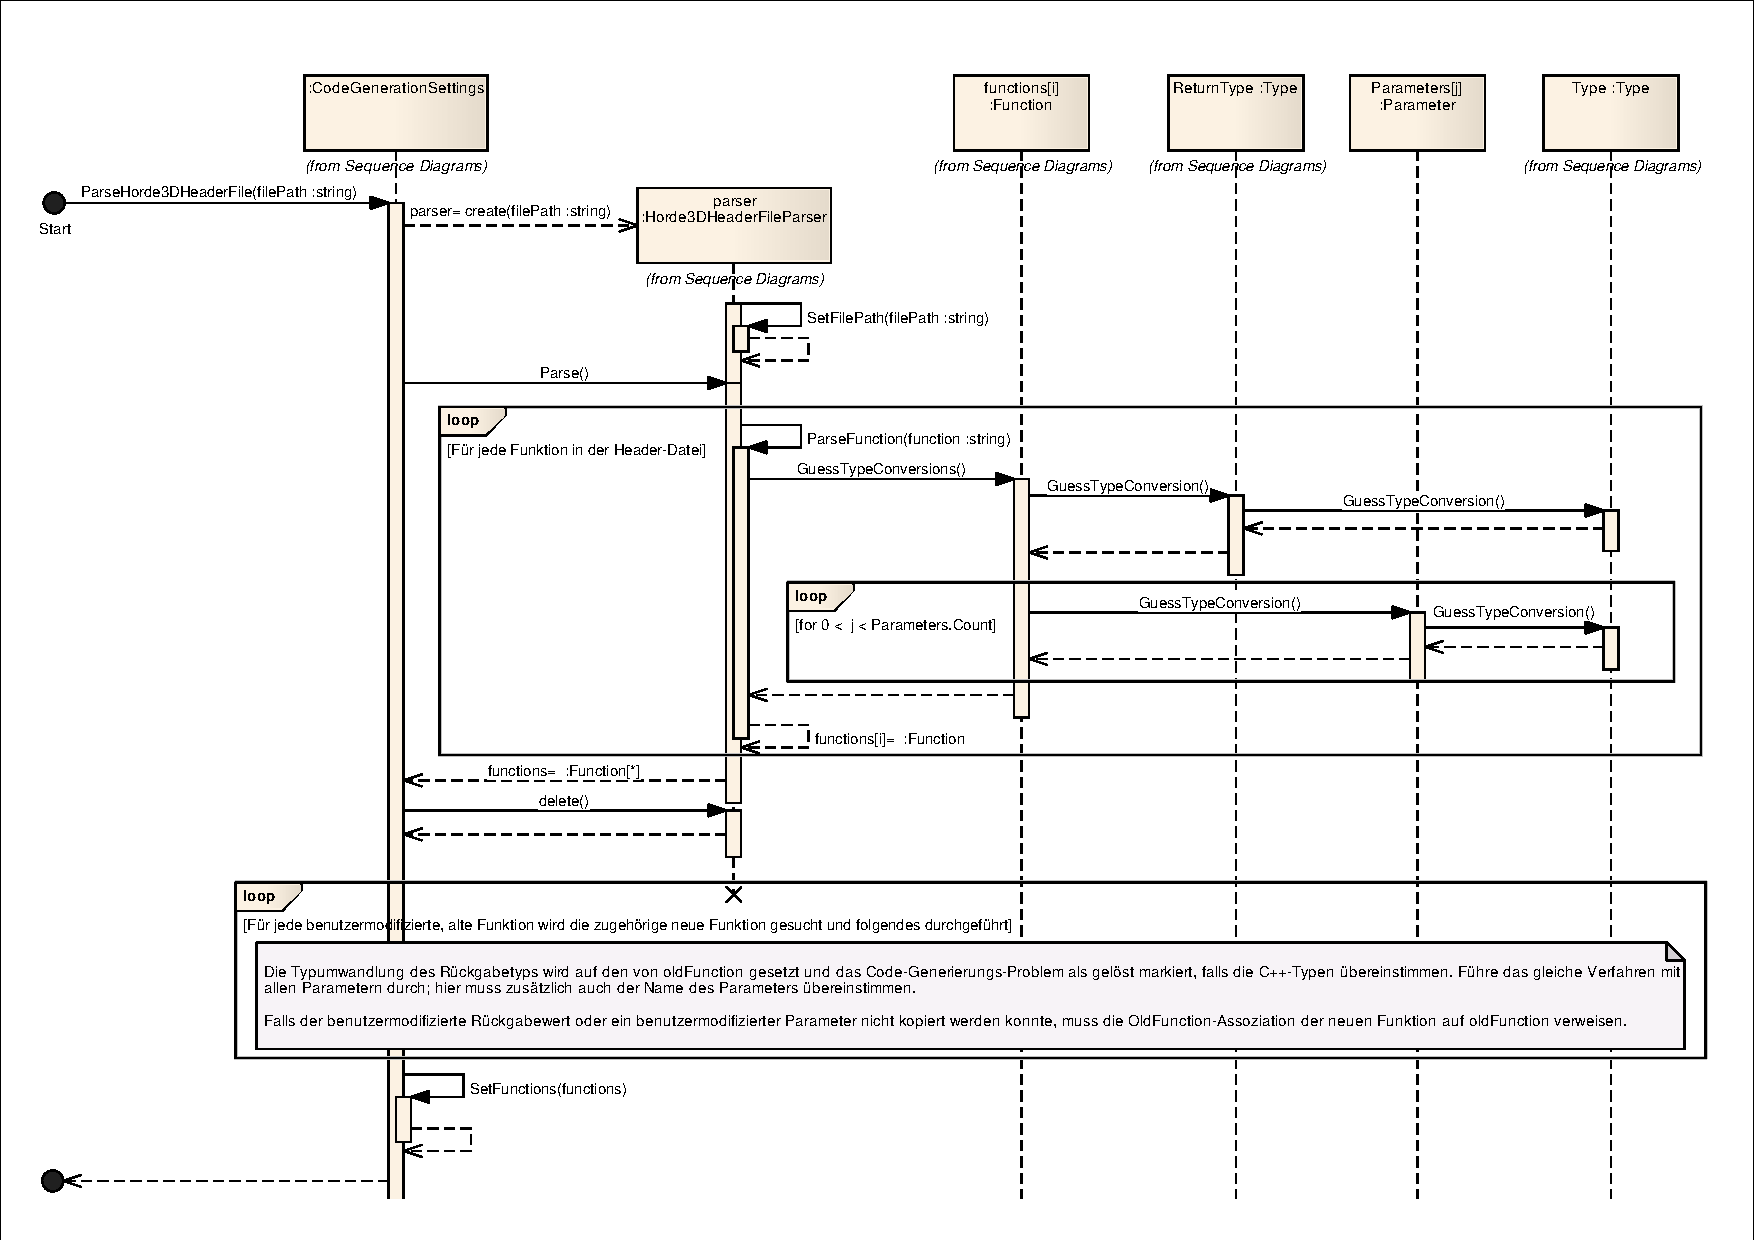
\includegraphics[trim = 1mm 1mm 1mm 1mm, clip, angle = 90, scale=0.7]{images/CodeGen_Parse.pdf}
\caption{Sequenzdiagramm f�r das Parsen der \emph{Header}-Datei}\label{fig:cgParse}
\end{figure}




\listoffigures

\flushleft
\nocite{*} 
\bibliographystyle{unsrt}
\bibliography{literatur} 




\end{document}

